% Options for packages loaded elsewhere
\PassOptionsToPackage{unicode}{hyperref}
\PassOptionsToPackage{hyphens}{url}
\PassOptionsToPackage{dvipsnames,svgnames,x11names}{xcolor}
%
\documentclass[
  letterpaper,
  DIV=11,
  numbers=noendperiod]{scrreprt}

\usepackage{amsmath,amssymb}
\usepackage{iftex}
\ifPDFTeX
  \usepackage[T1]{fontenc}
  \usepackage[utf8]{inputenc}
  \usepackage{textcomp} % provide euro and other symbols
\else % if luatex or xetex
  \usepackage{unicode-math}
  \defaultfontfeatures{Scale=MatchLowercase}
  \defaultfontfeatures[\rmfamily]{Ligatures=TeX,Scale=1}
\fi
\usepackage{lmodern}
\ifPDFTeX\else  
    % xetex/luatex font selection
\fi
% Use upquote if available, for straight quotes in verbatim environments
\IfFileExists{upquote.sty}{\usepackage{upquote}}{}
\IfFileExists{microtype.sty}{% use microtype if available
  \usepackage[]{microtype}
  \UseMicrotypeSet[protrusion]{basicmath} % disable protrusion for tt fonts
}{}
\makeatletter
\@ifundefined{KOMAClassName}{% if non-KOMA class
  \IfFileExists{parskip.sty}{%
    \usepackage{parskip}
  }{% else
    \setlength{\parindent}{0pt}
    \setlength{\parskip}{6pt plus 2pt minus 1pt}}
}{% if KOMA class
  \KOMAoptions{parskip=half}}
\makeatother
\usepackage{xcolor}
\setlength{\emergencystretch}{3em} % prevent overfull lines
\setcounter{secnumdepth}{5}
% Make \paragraph and \subparagraph free-standing
\ifx\paragraph\undefined\else
  \let\oldparagraph\paragraph
  \renewcommand{\paragraph}[1]{\oldparagraph{#1}\mbox{}}
\fi
\ifx\subparagraph\undefined\else
  \let\oldsubparagraph\subparagraph
  \renewcommand{\subparagraph}[1]{\oldsubparagraph{#1}\mbox{}}
\fi


\providecommand{\tightlist}{%
  \setlength{\itemsep}{0pt}\setlength{\parskip}{0pt}}\usepackage{longtable,booktabs,array}
\usepackage{calc} % for calculating minipage widths
% Correct order of tables after \paragraph or \subparagraph
\usepackage{etoolbox}
\makeatletter
\patchcmd\longtable{\par}{\if@noskipsec\mbox{}\fi\par}{}{}
\makeatother
% Allow footnotes in longtable head/foot
\IfFileExists{footnotehyper.sty}{\usepackage{footnotehyper}}{\usepackage{footnote}}
\makesavenoteenv{longtable}
\usepackage{graphicx}
\makeatletter
\def\maxwidth{\ifdim\Gin@nat@width>\linewidth\linewidth\else\Gin@nat@width\fi}
\def\maxheight{\ifdim\Gin@nat@height>\textheight\textheight\else\Gin@nat@height\fi}
\makeatother
% Scale images if necessary, so that they will not overflow the page
% margins by default, and it is still possible to overwrite the defaults
% using explicit options in \includegraphics[width, height, ...]{}
\setkeys{Gin}{width=\maxwidth,height=\maxheight,keepaspectratio}
% Set default figure placement to htbp
\makeatletter
\def\fps@figure{htbp}
\makeatother

\KOMAoption{captions}{tableheading}
\makeatletter
\@ifpackageloaded{tcolorbox}{}{\usepackage[skins,breakable]{tcolorbox}}
\@ifpackageloaded{fontawesome5}{}{\usepackage{fontawesome5}}
\definecolor{quarto-callout-color}{HTML}{909090}
\definecolor{quarto-callout-note-color}{HTML}{0758E5}
\definecolor{quarto-callout-important-color}{HTML}{CC1914}
\definecolor{quarto-callout-warning-color}{HTML}{EB9113}
\definecolor{quarto-callout-tip-color}{HTML}{00A047}
\definecolor{quarto-callout-caution-color}{HTML}{FC5300}
\definecolor{quarto-callout-color-frame}{HTML}{acacac}
\definecolor{quarto-callout-note-color-frame}{HTML}{4582ec}
\definecolor{quarto-callout-important-color-frame}{HTML}{d9534f}
\definecolor{quarto-callout-warning-color-frame}{HTML}{f0ad4e}
\definecolor{quarto-callout-tip-color-frame}{HTML}{02b875}
\definecolor{quarto-callout-caution-color-frame}{HTML}{fd7e14}
\makeatother
\makeatletter
\@ifpackageloaded{bookmark}{}{\usepackage{bookmark}}
\makeatother
\makeatletter
\@ifpackageloaded{caption}{}{\usepackage{caption}}
\AtBeginDocument{%
\ifdefined\contentsname
  \renewcommand*\contentsname{Table of contents}
\else
  \newcommand\contentsname{Table of contents}
\fi
\ifdefined\listfigurename
  \renewcommand*\listfigurename{List of Figures}
\else
  \newcommand\listfigurename{List of Figures}
\fi
\ifdefined\listtablename
  \renewcommand*\listtablename{List of Tables}
\else
  \newcommand\listtablename{List of Tables}
\fi
\ifdefined\figurename
  \renewcommand*\figurename{Figure}
\else
  \newcommand\figurename{Figure}
\fi
\ifdefined\tablename
  \renewcommand*\tablename{Table}
\else
  \newcommand\tablename{Table}
\fi
}
\@ifpackageloaded{float}{}{\usepackage{float}}
\floatstyle{ruled}
\@ifundefined{c@chapter}{\newfloat{codelisting}{h}{lop}}{\newfloat{codelisting}{h}{lop}[chapter]}
\floatname{codelisting}{Listing}
\newcommand*\listoflistings{\listof{codelisting}{List of Listings}}
\makeatother
\makeatletter
\makeatother
\makeatletter
\@ifpackageloaded{caption}{}{\usepackage{caption}}
\@ifpackageloaded{subcaption}{}{\usepackage{subcaption}}
\makeatother
\ifLuaTeX
  \usepackage{selnolig}  % disable illegal ligatures
\fi
\usepackage{bookmark}

\IfFileExists{xurl.sty}{\usepackage{xurl}}{} % add URL line breaks if available
\urlstyle{same} % disable monospaced font for URLs
\hypersetup{
  pdftitle={Data Analysis with SPSS},
  pdfauthor={Kamarul Ariffin Mansor},
  colorlinks=true,
  linkcolor={blue},
  filecolor={Maroon},
  citecolor={Blue},
  urlcolor={Blue},
  pdfcreator={LaTeX via pandoc}}

\title{Data Analysis with SPSS}
\author{Kamarul Ariffin Mansor}
\date{2025-01-12}

\begin{document}
\maketitle

\renewcommand*\contentsname{Table of contents}
{
\hypersetup{linkcolor=}
\setcounter{tocdepth}{2}
\tableofcontents
}
\bookmarksetup{startatroot}

\chapter*{Preface}\label{preface}
\addcontentsline{toc}{chapter}{Preface}

\markboth{Preface}{Preface}

Statistical Package for the Social Science (SPSS)\\
\strut \\
Conducted by:\\
\strut \\
Kamarul Ariffin Mansor\\
Senior Lecturer\\
Universiti Teknologi MARA (UiTM)\\
Kedah Branch Campus\\
Malaysia\\

This module provides a comprehensive guide to conducting data analysis
using SPSS, a widely used statistical software. It is structured into a
step-by-step process that covers the entire workflow, from data
preparation to advanced statistical tests. Key components include:\\

\begin{enumerate}
\def\labelenumi{\arabic{enumi}.}
\tightlist
\item
  \textbf{Introduction:} An overview of SPSS software and its role in
  statistical analysis. Data Inputs in SPSS Software: Instructions on
  importing and organizing data within SPSS, including file formats and
  data entry techniques.\\
\item
  \textbf{Data Transformation:} Techniques to prepare data for analysis,
  such as recoding variables and computing new ones.\\
\item
  \textbf{Descriptive Statistics:} Procedures for summarizing and
  describing data distributions, including measures of central tendency
  and dispersion.\\
\item
  \textbf{Test of Data Normality:} Methods for assessing the normality
  of data using skewness and kurtosis.\\
\item
  \textbf{Test of Outliers:} Identification and handling of outliers in
  both univariate and multivariate data sets.\\
\item
  \textbf{Test of Data Reliability:} Evaluation of the internal
  consistency of scales using Cronbach's Alpha.\\
\item
  \textbf{Exploratory Factor Analysis (EFA):} Techniques to uncover
  underlying structures in the data and reduce dimensionality.\\
\item
  \textbf{T-Tests:} Application of one-sample, independent sample, and
  paired sample t-tests to compare means across groups or conditions.\\
\item
  \textbf{ANOVA Tests:} Use of one-way, two-way, and repeated-measures
  ANOVA for analyzing variance among multiple groups.\\
\item
  \textbf{Correlation Tests:} Examination of relationships between
  variables using correlation coefficients.\\
\item
  \textbf{Regression Analysis:} Implementation of simple and multiple
  linear regression to model relationships between dependent and
  independent variables.\\
  \strut \\
  The module equips users with practical knowledge and step-by-step
  guidance to conduct data analysis in SPSS effectively, catering to
  both beginners and intermediate users. It emphasizes the integration
  of statistical theory with practical application, making it a valuable
  resource for researchers, students, and professionals in various
  fields.\\
\end{enumerate}

\textbf{Research Framework}\\

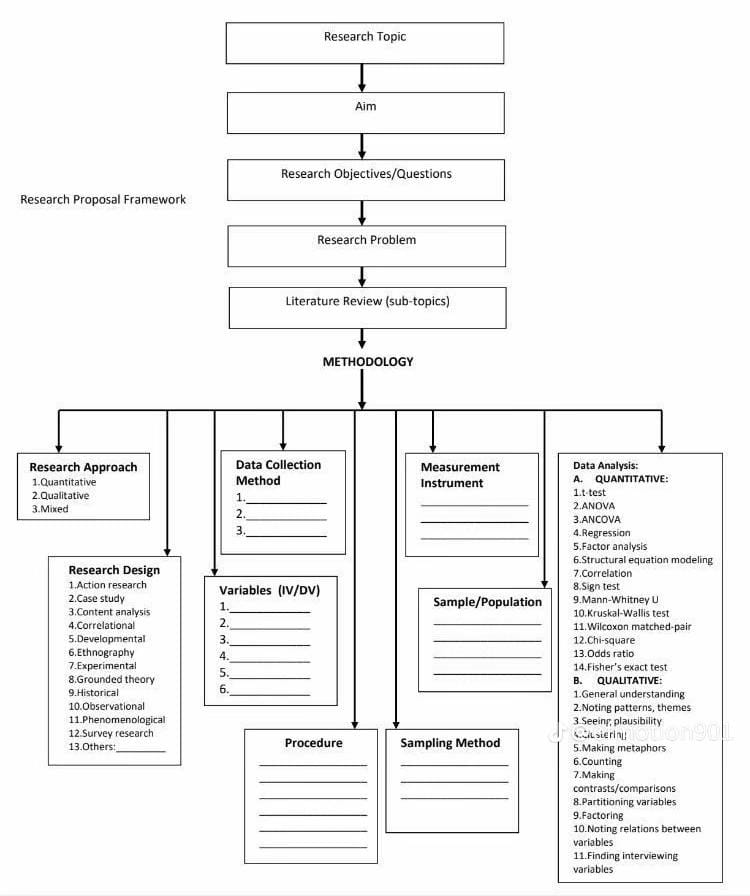
\includegraphics{images/framework.jpeg}

\textbf{What is SPSS?}\\

• Originally it is an acronym of Statistical Package for the Social
Science but now it stands for Statistical Product and Service
Solutions\\
• One of the most popular statistical packages which can perform highly
complex data manipulation and analysis with simple instructions\\

\textbf{SPSS Version}\\

-- The earlier versions of SPSS ran on mainframe computers\\
- SPSS 1 - 1968\\
- SPSS 2 - 1983\\
-- SPSS/PC+ was first introduced in 1984\\
- SPSS 5 - 1993\\
-- SPSS 6 for Windows was introduced in mid 1990's\\
- SPSS 6.1 - 1995\\
- SPSS 7.5 - 1997\\
- SPSS 8 - 1998\\
- SPSS 9 - 1999\\
- SPSS 10 - 1999\\
- SPSS 11 - 2002\\
- SPSS 12 - 2004\\
- SPSS 13 - 2005\\
- SPSS 14 - 2006\\
-- SPSS 15 - November 2006\\
-- SPSS 16 - April 2008\\
-- PASW Statistics 17 -- December 2008\\
-- PASW Statistics 18 -- August 2009\\
-- SPSS Statistics 19 -- 2010\\
-- SPSS Statistics 20 -- 2011\\
-- SPSS Statistics 21 -- 2012\\
-- SPSS Statistics 22 -- 2013\\
-- SPSS Statistics 23 -- 2015\\
- SPSS 24 - 2016, March\\
- SPSS 25 - 2017, July\\
- SPSS 26 - 2018\\
- SPSS 27 - 2019, June (and 27.0.1 in November, 2020)\\
- SPSS 28 - 2021, May\\
- SPSS 29 - 2022, Sept\\
- SPSS 30 - 2024, Sept\\

SPSS is a software used for statistical analysis\\
First released in 1968 and was developed by Normane H. Bent and C.
Hadial Hull\\
Since its release, SPSS was under SPSS Inc.\\
However in July 28, 2009 SPSS was acquired by IBM for US\$1.2 billion\\
Versions 17 and 18 were known as PASW (Predictive and Analytical
Software)\\
Version 19 was renamed as SPSS Statistics\\

\textbf{Contents:}\\
\textbf{Step by Step Data Analysis Process by SPSS}\\

\begin{enumerate}
\def\labelenumi{\arabic{enumi}.}
\tightlist
\item
  Introduction\\
\item
  Data Inputs in SPSS Software\\
\item
  Data Transformation\\
\item
  Descriptive Statistics\\
\item
  Test of Data Normality (skewness \& kurtosis)\\
\item
  Test of Outliers (univariate \& multivariate)\\
\item
  Test of Data Reliability (Cronbach's Alpha)\\
\item
  Exploratory Factor Analysis (EFA)\\
\item
  T-Tests (one sample, independent sample t-test, and paired sample
  t-test)\\
\item
  ANOVA Tests (one-way, two-way, and repetitive measure ANOVA)\\
\item
  Correlation Tests\\
\item
  Regressions Analysis (Simple, and Multiple Linear Regression)\\
\end{enumerate}

\bookmarksetup{startatroot}

\chapter{Introduction}\label{introduction}

\section{Types of Variables}\label{types-of-variables}


\includegraphics{images/bicycle.png}

What are variables you would consider in buying a second hand bike?\\

\begin{itemize}
\tightlist
\item
  Brand (Trek, Raleigh)\\
\item
  Type (road, mountain, racer)\\
\item
  Components (Shimano, no name)\\
\item
  Age\\
\item
  Condition (Excellent, good, poor)\\
\item
  Price\\
\item
  Frame size\\
\item
  Number of gears\\
\end{itemize}

\section{Parametric vs
Non-parametric}\label{parametric-vs-non-parametric}

\begin{itemize}
\tightlist
\item
  Parametric stats are more powerful than non-parametric stats- for real
  numbers- example like t-test\\
\item
  Non-parametric stats are not as powerful but good for category
  variables -- example like Mann-Whitney U (Likert)\\
\end{itemize}

\section{Types of Scales}\label{types-of-scales}

\begin{tcolorbox}[enhanced jigsaw, rightrule=.15mm, arc=.35mm, colframe=quarto-callout-tip-color-frame, coltitle=black, left=2mm, colbacktitle=quarto-callout-tip-color!10!white, bottomtitle=1mm, titlerule=0mm, colback=white, breakable, opacitybacktitle=0.6, opacityback=0, toprule=.15mm, toptitle=1mm, title=\textcolor{quarto-callout-tip-color}{\faLightbulb}\hspace{0.5em}{Nominal}, bottomrule=.15mm, leftrule=.75mm]

objects or people are categorized according to some criterion (gender,
job category)

\end{tcolorbox}

\begin{tcolorbox}[enhanced jigsaw, rightrule=.15mm, arc=.35mm, colframe=quarto-callout-tip-color-frame, coltitle=black, left=2mm, colbacktitle=quarto-callout-tip-color!10!white, bottomtitle=1mm, titlerule=0mm, colback=white, breakable, opacitybacktitle=0.6, opacityback=0, toprule=.15mm, toptitle=1mm, title=\textcolor{quarto-callout-tip-color}{\faLightbulb}\hspace{0.5em}{Ordinal}, bottomrule=.15mm, leftrule=.75mm]

Categories which are ranked according to characteristics (income- low,
moderate, high)

\end{tcolorbox}

\begin{tcolorbox}[enhanced jigsaw, rightrule=.15mm, arc=.35mm, colframe=quarto-callout-tip-color-frame, coltitle=black, left=2mm, colbacktitle=quarto-callout-tip-color!10!white, bottomtitle=1mm, titlerule=0mm, colback=white, breakable, opacitybacktitle=0.6, opacityback=0, toprule=.15mm, toptitle=1mm, title=\textcolor{quarto-callout-tip-color}{\faLightbulb}\hspace{0.5em}{Interval}, bottomrule=.15mm, leftrule=.75mm]

contain equal distance between units of measure- but no zero (calendar
years, temperature)

\end{tcolorbox}

\begin{tcolorbox}[enhanced jigsaw, rightrule=.15mm, arc=.35mm, colframe=quarto-callout-tip-color-frame, coltitle=black, left=2mm, colbacktitle=quarto-callout-tip-color!10!white, bottomtitle=1mm, titlerule=0mm, colback=white, breakable, opacitybacktitle=0.6, opacityback=0, toprule=.15mm, toptitle=1mm, title=\textcolor{quarto-callout-tip-color}{\faLightbulb}\hspace{0.5em}{Ratio}, bottomrule=.15mm, leftrule=.75mm]

has an absolute zero and consistent intervals (distance, weight)

\end{tcolorbox}

\bookmarksetup{startatroot}

\chapter{Data Input in SPSS}\label{data-input-in-spss}

The following are the most common data input when doing a survey
research.\\

\section{Data Inputs from Questionnaire to
SPSS}\label{data-inputs-from-questionnaire-to-spss}

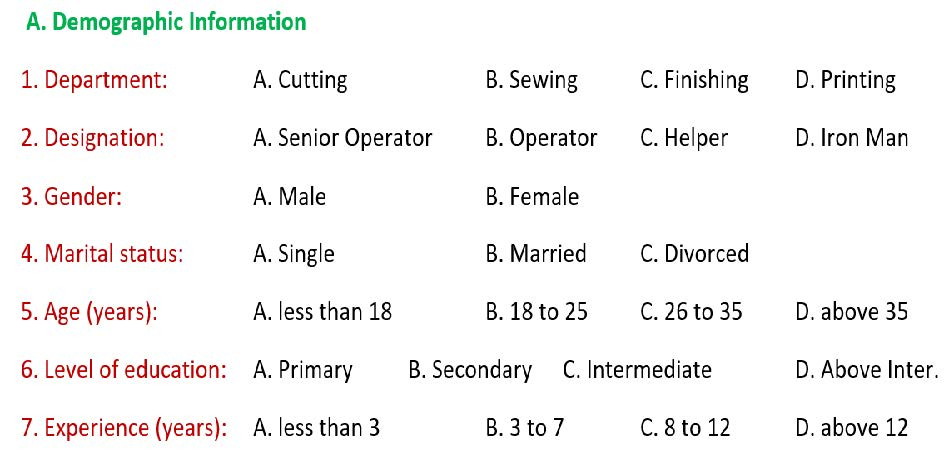
\includegraphics{images/demographic.jpg}

\section{Likert Scale Data}\label{likert-scale-data}

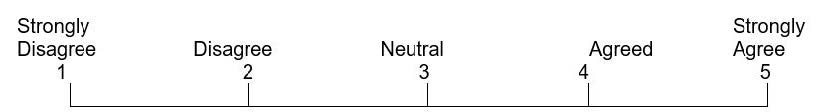
\includegraphics{images/scale.jpg}

\textbf{ATTITUDE}\\
This section is to understand your feelings towards knowledge sharing.
Please circle the appropriate number on each scale.\\

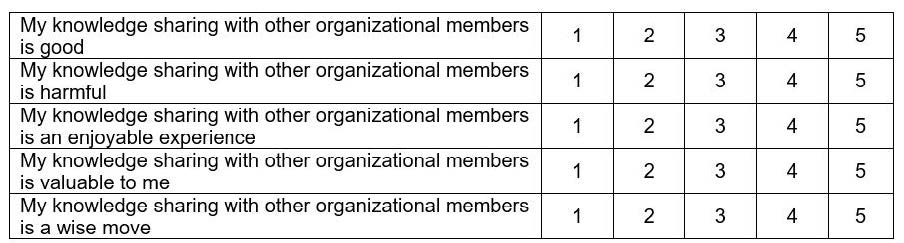
\includegraphics{images/attitude.jpg}

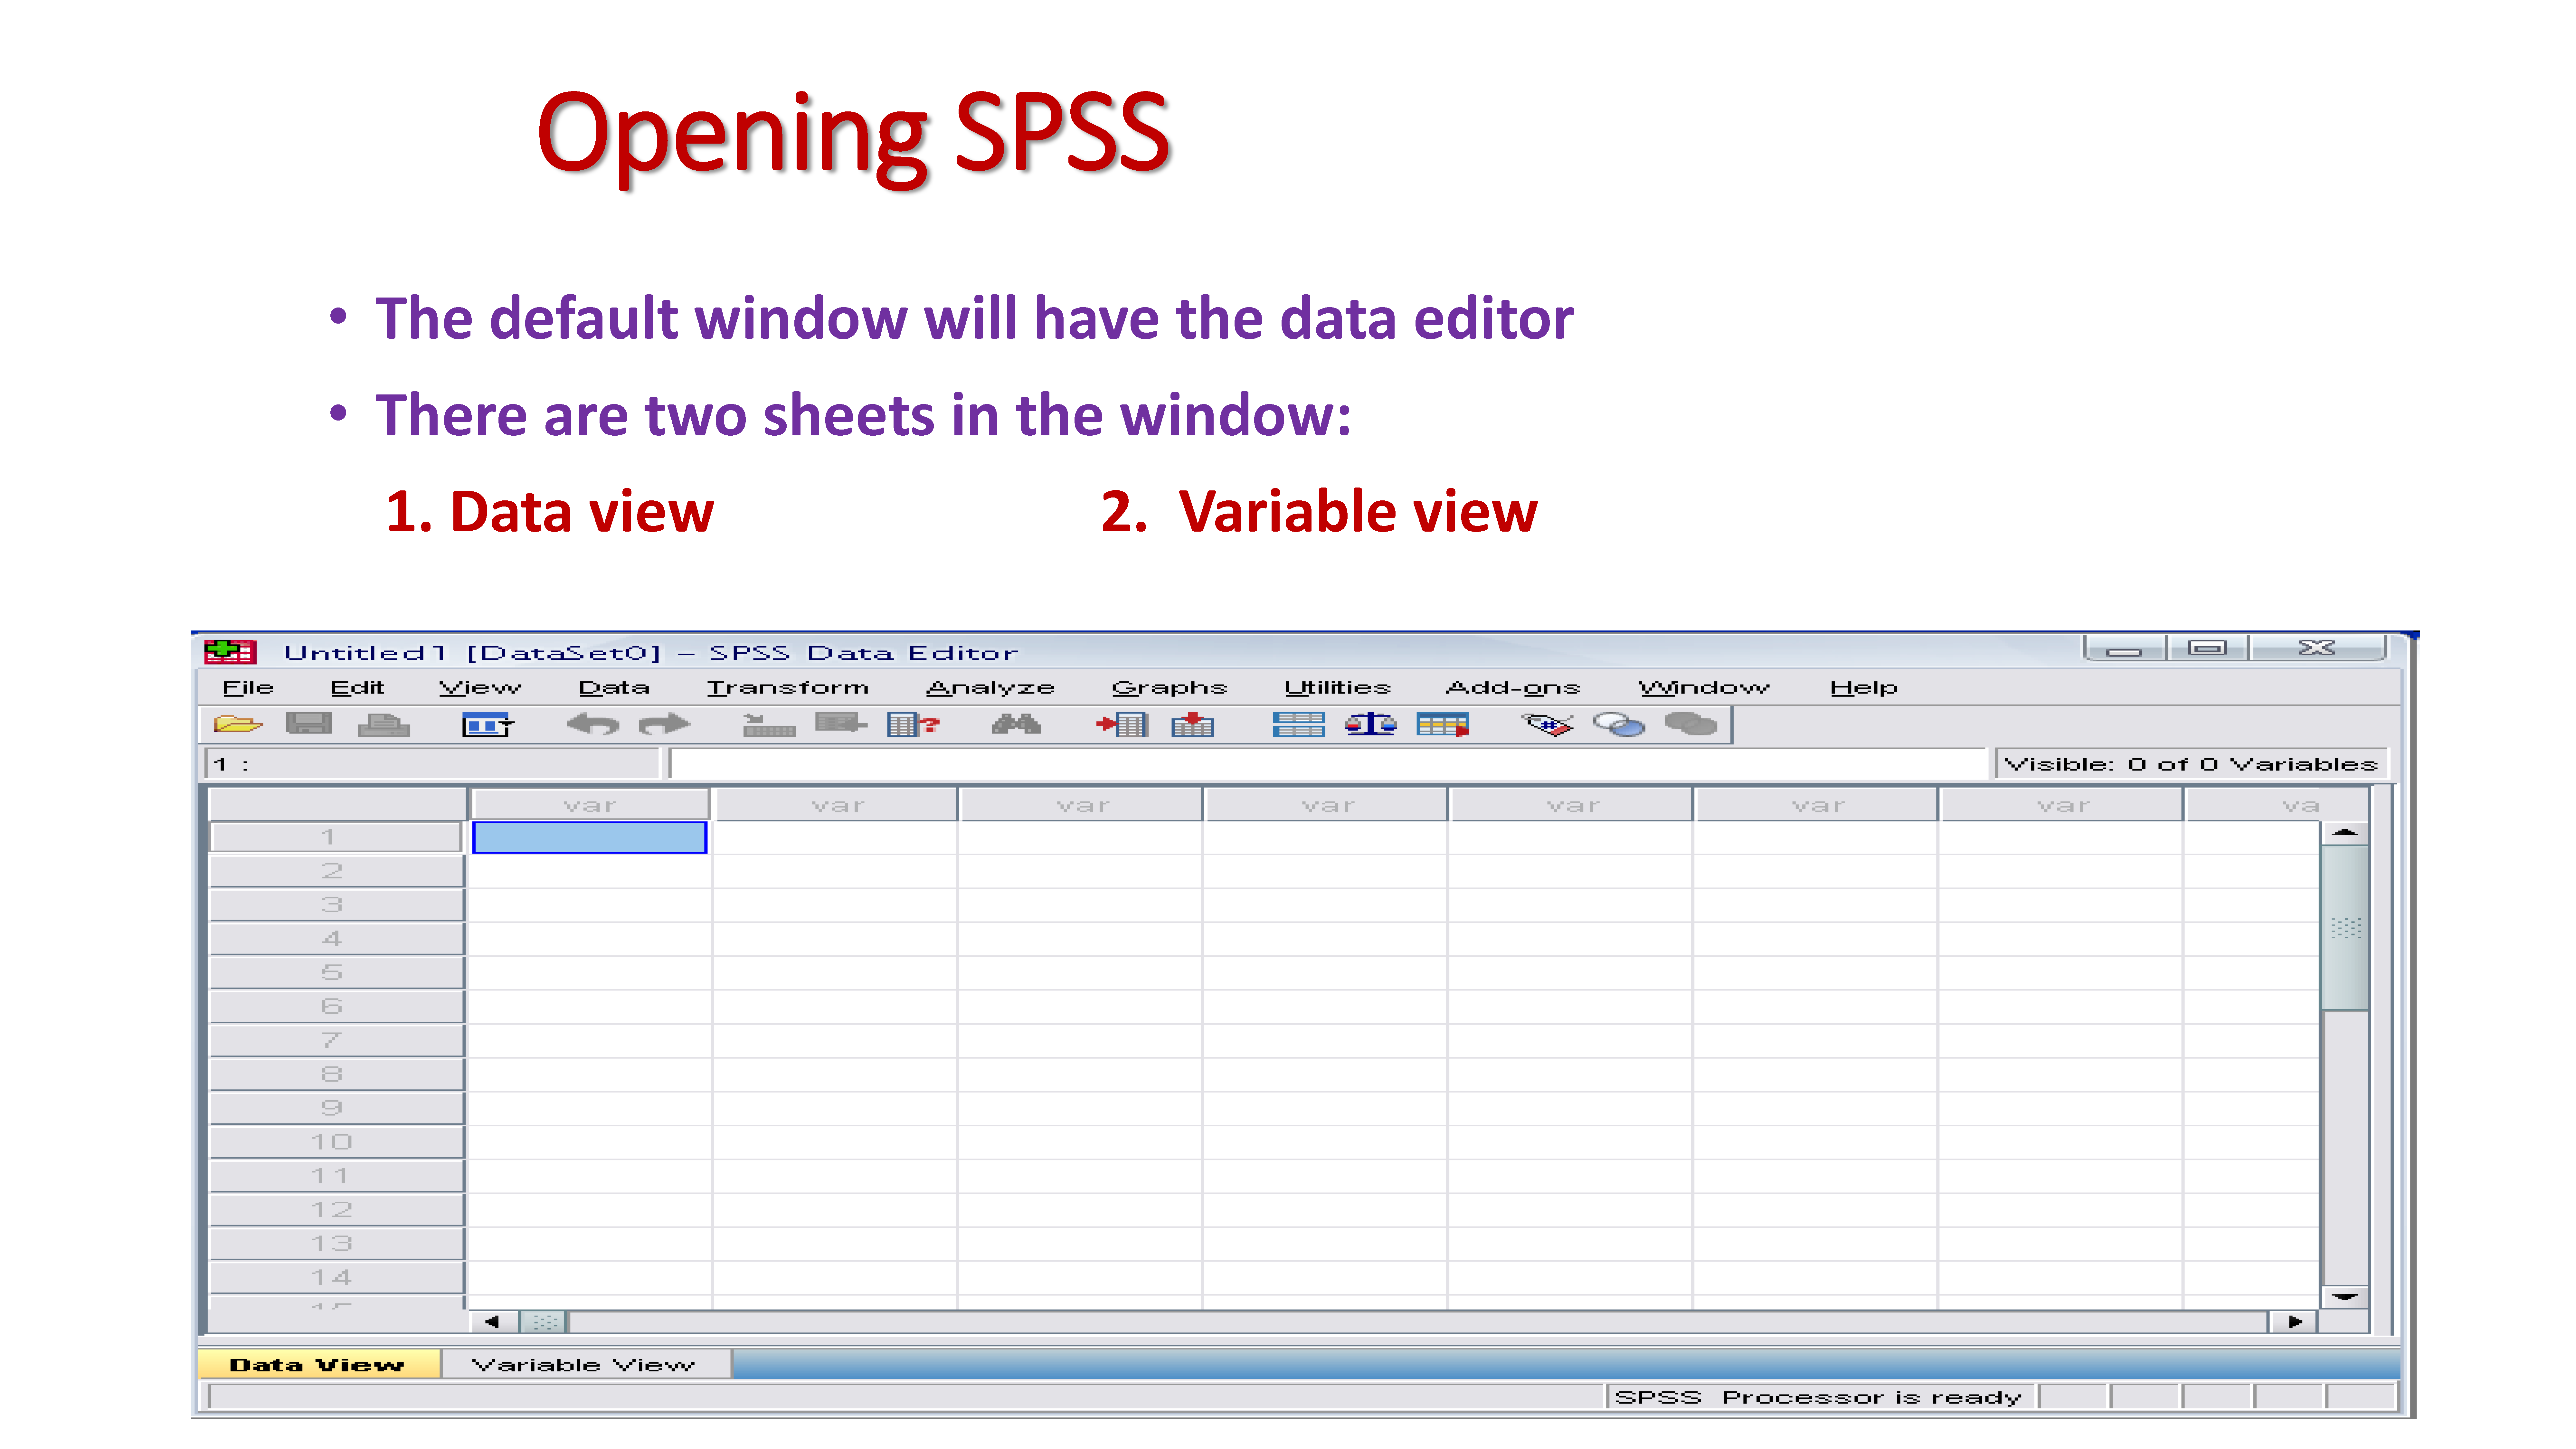
\includegraphics{images/slides/img_Page_013.png}

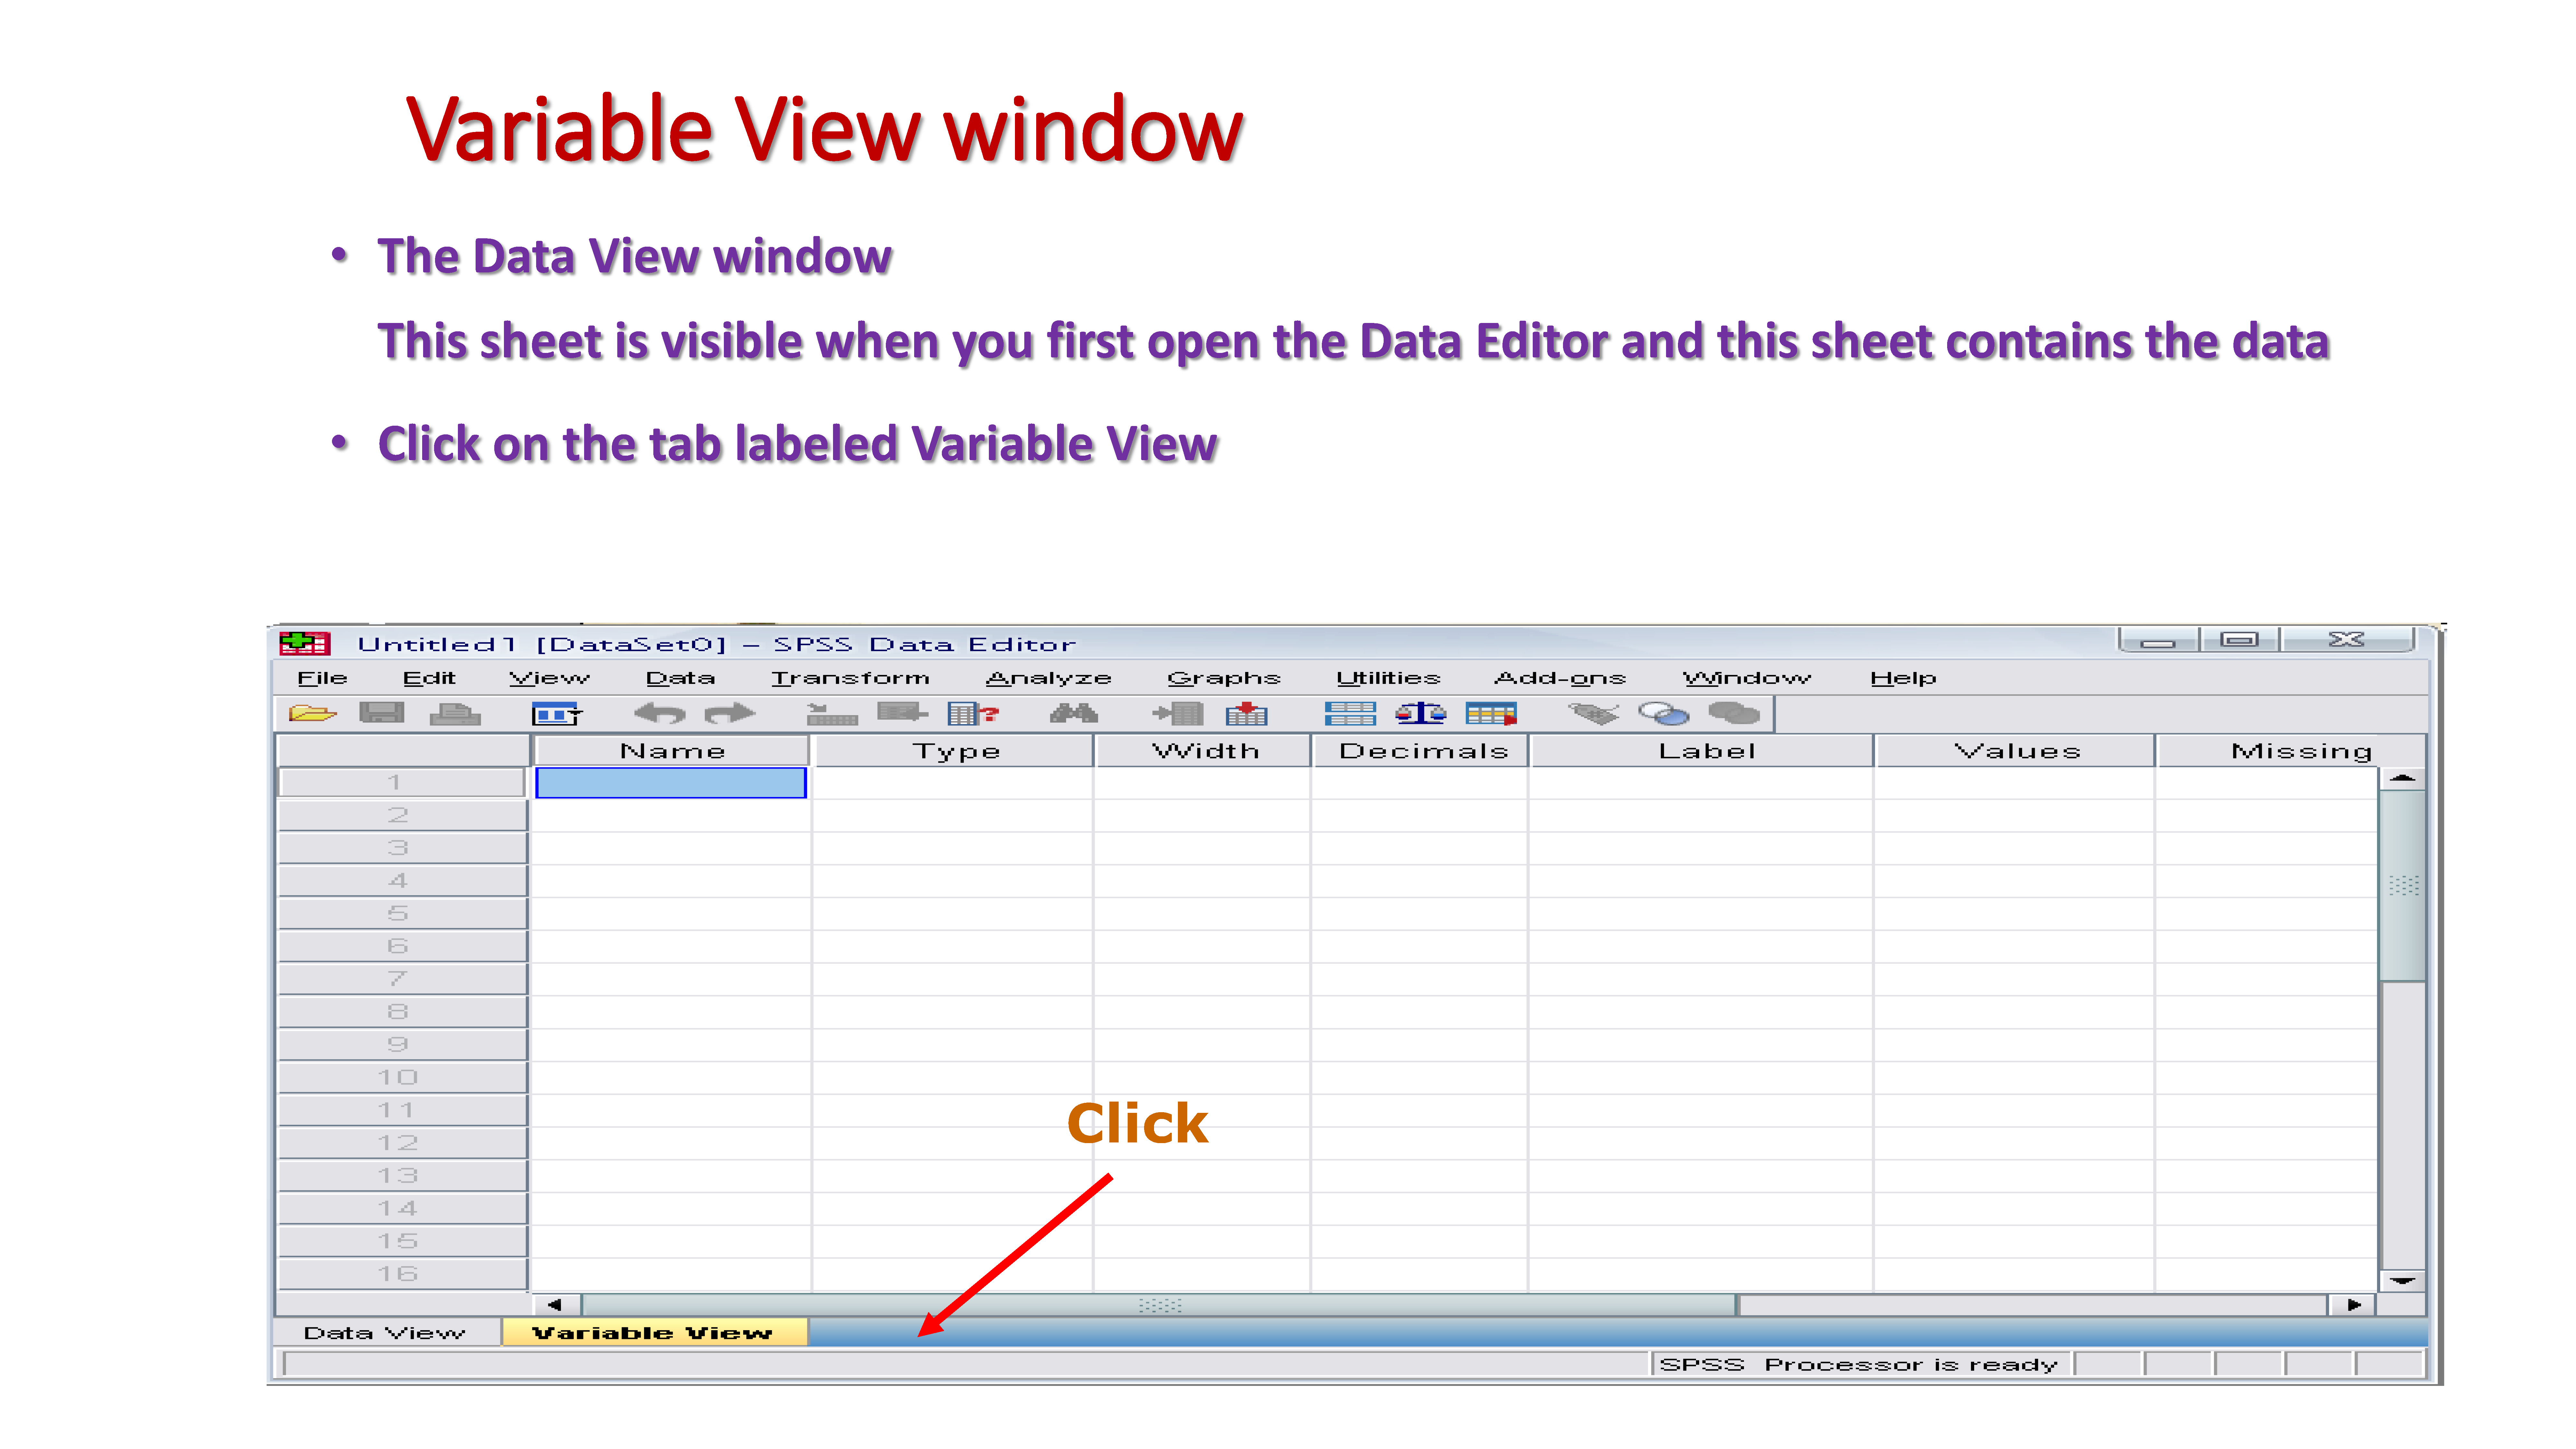
\includegraphics{images/slides/img_Page_014.png}

\bookmarksetup{startatroot}

\chapter{Data Transformation}\label{data-transformation}

To transform data, you perform a mathematical operation on each
observation, then use these transformed numbers in your statistical
test.\\

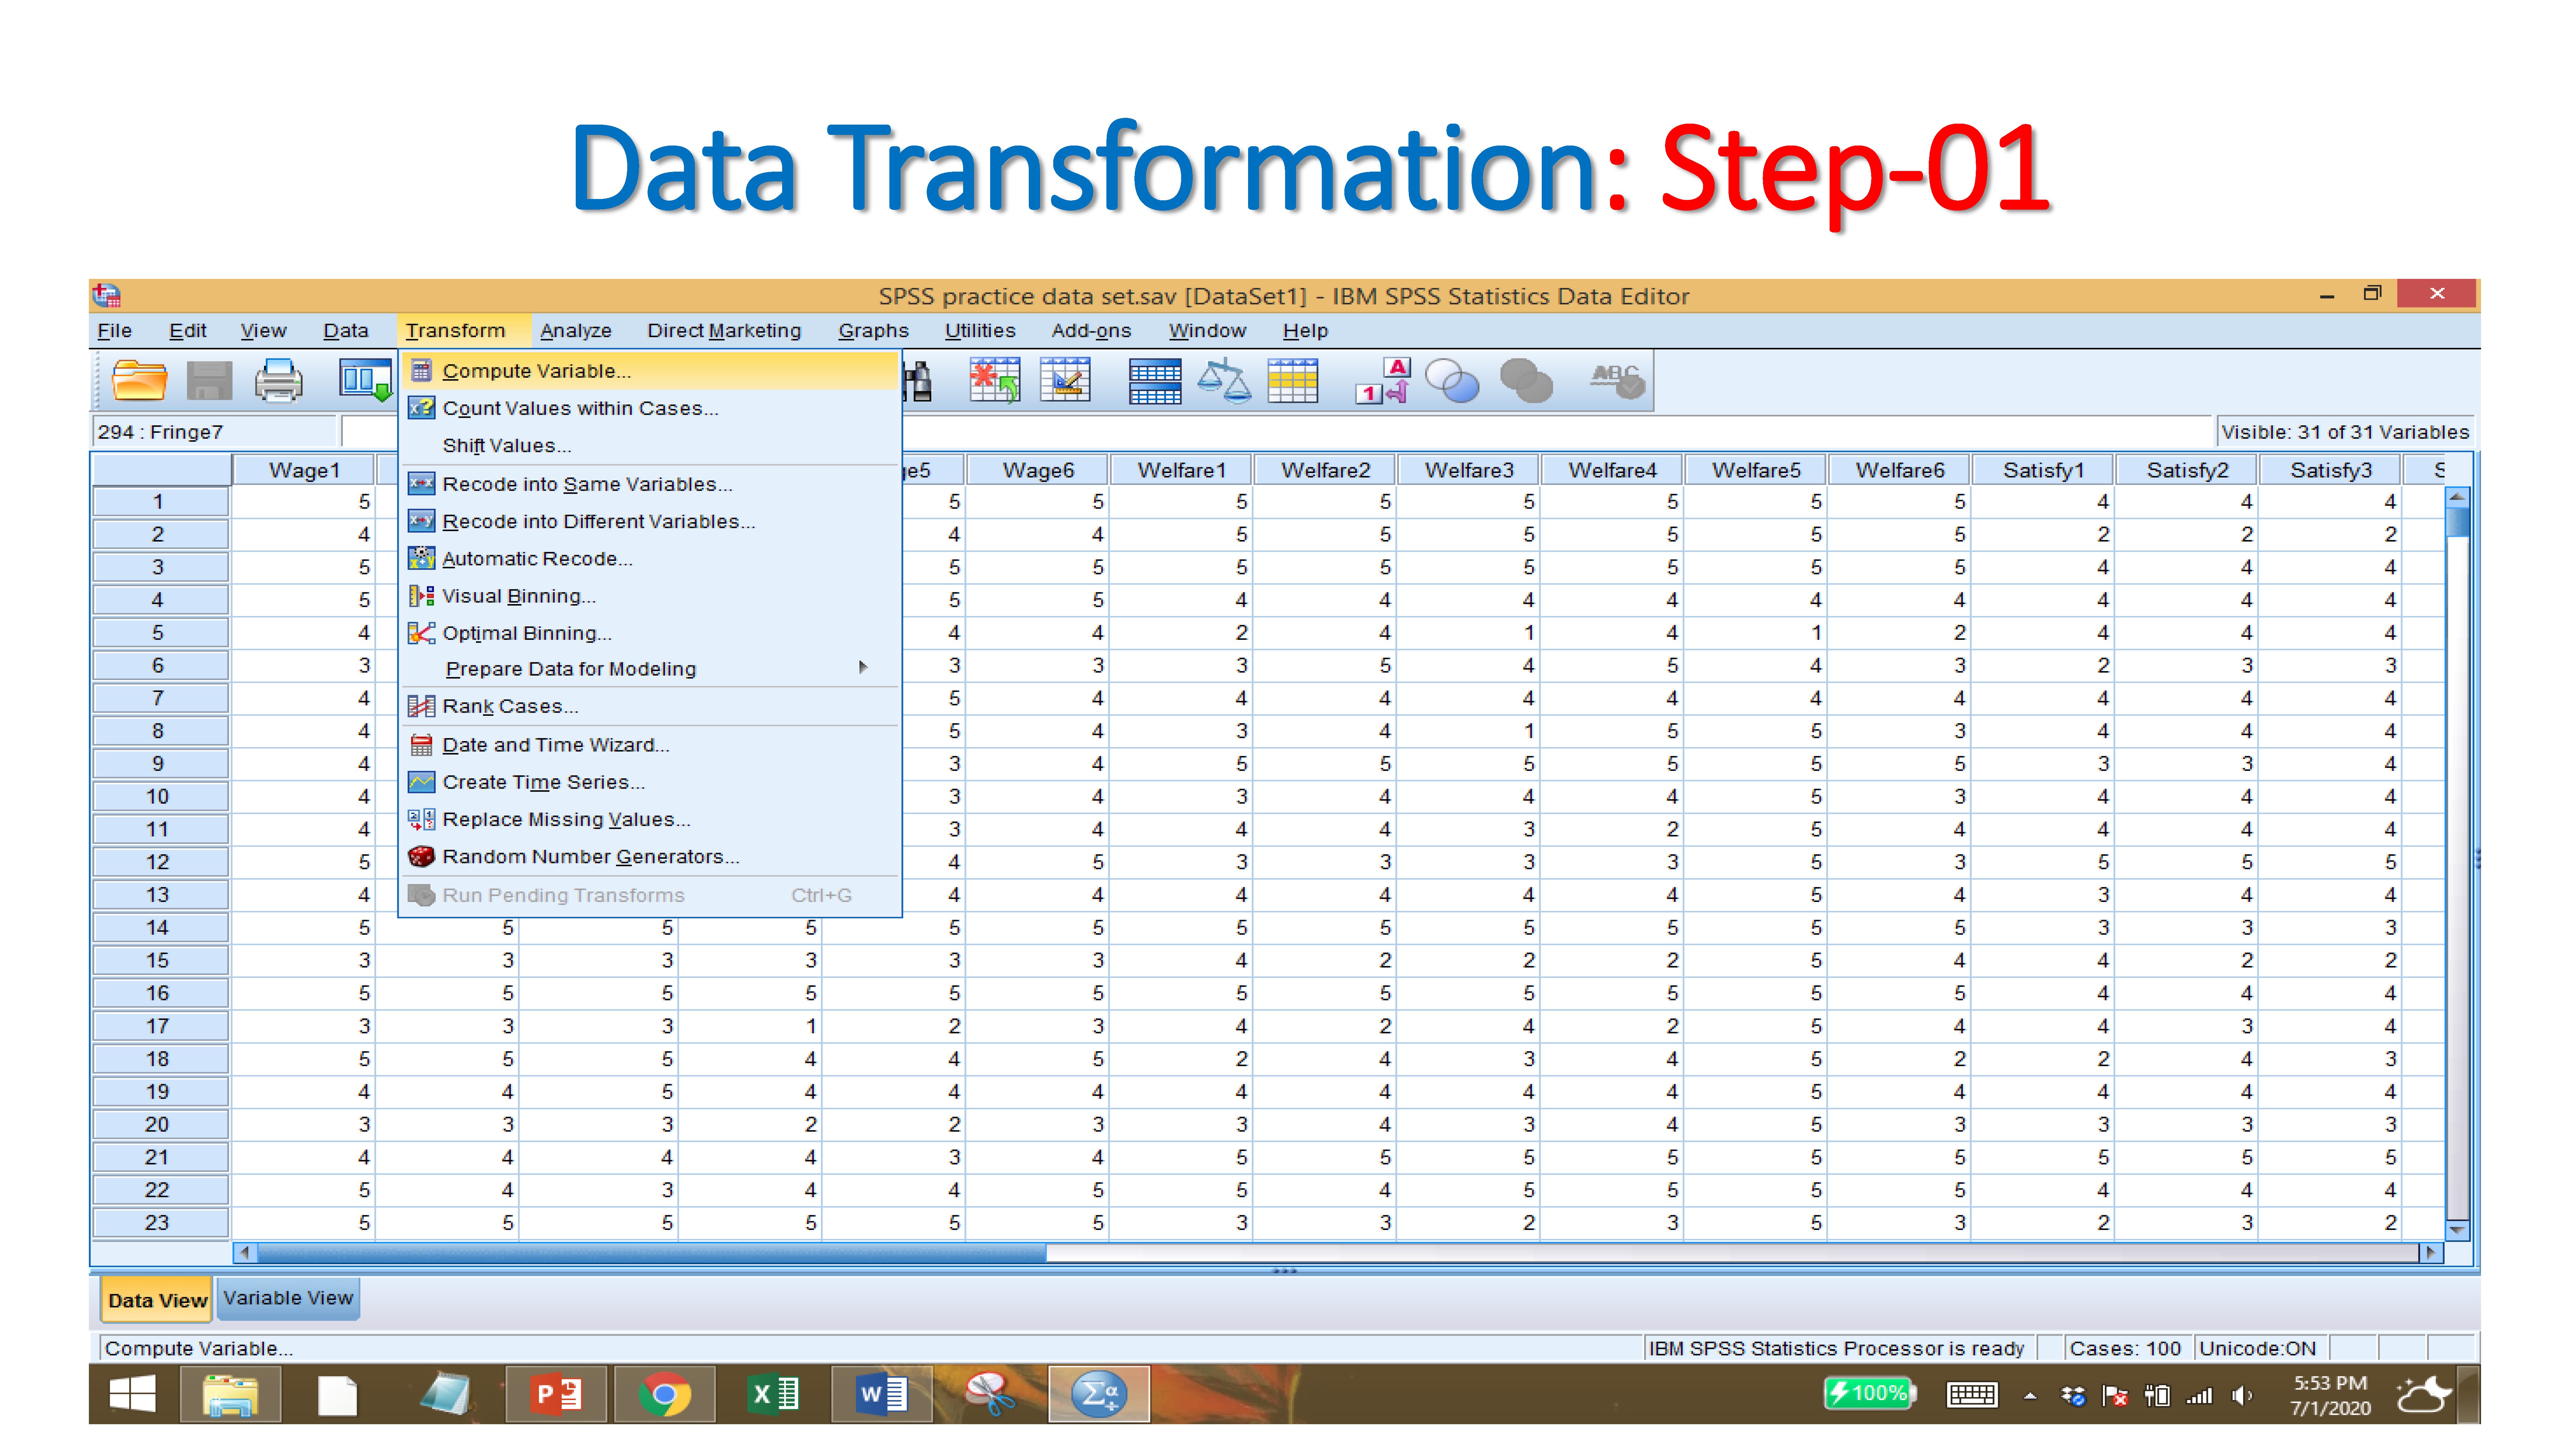
\includegraphics{images/slides/img_Page_016.png}

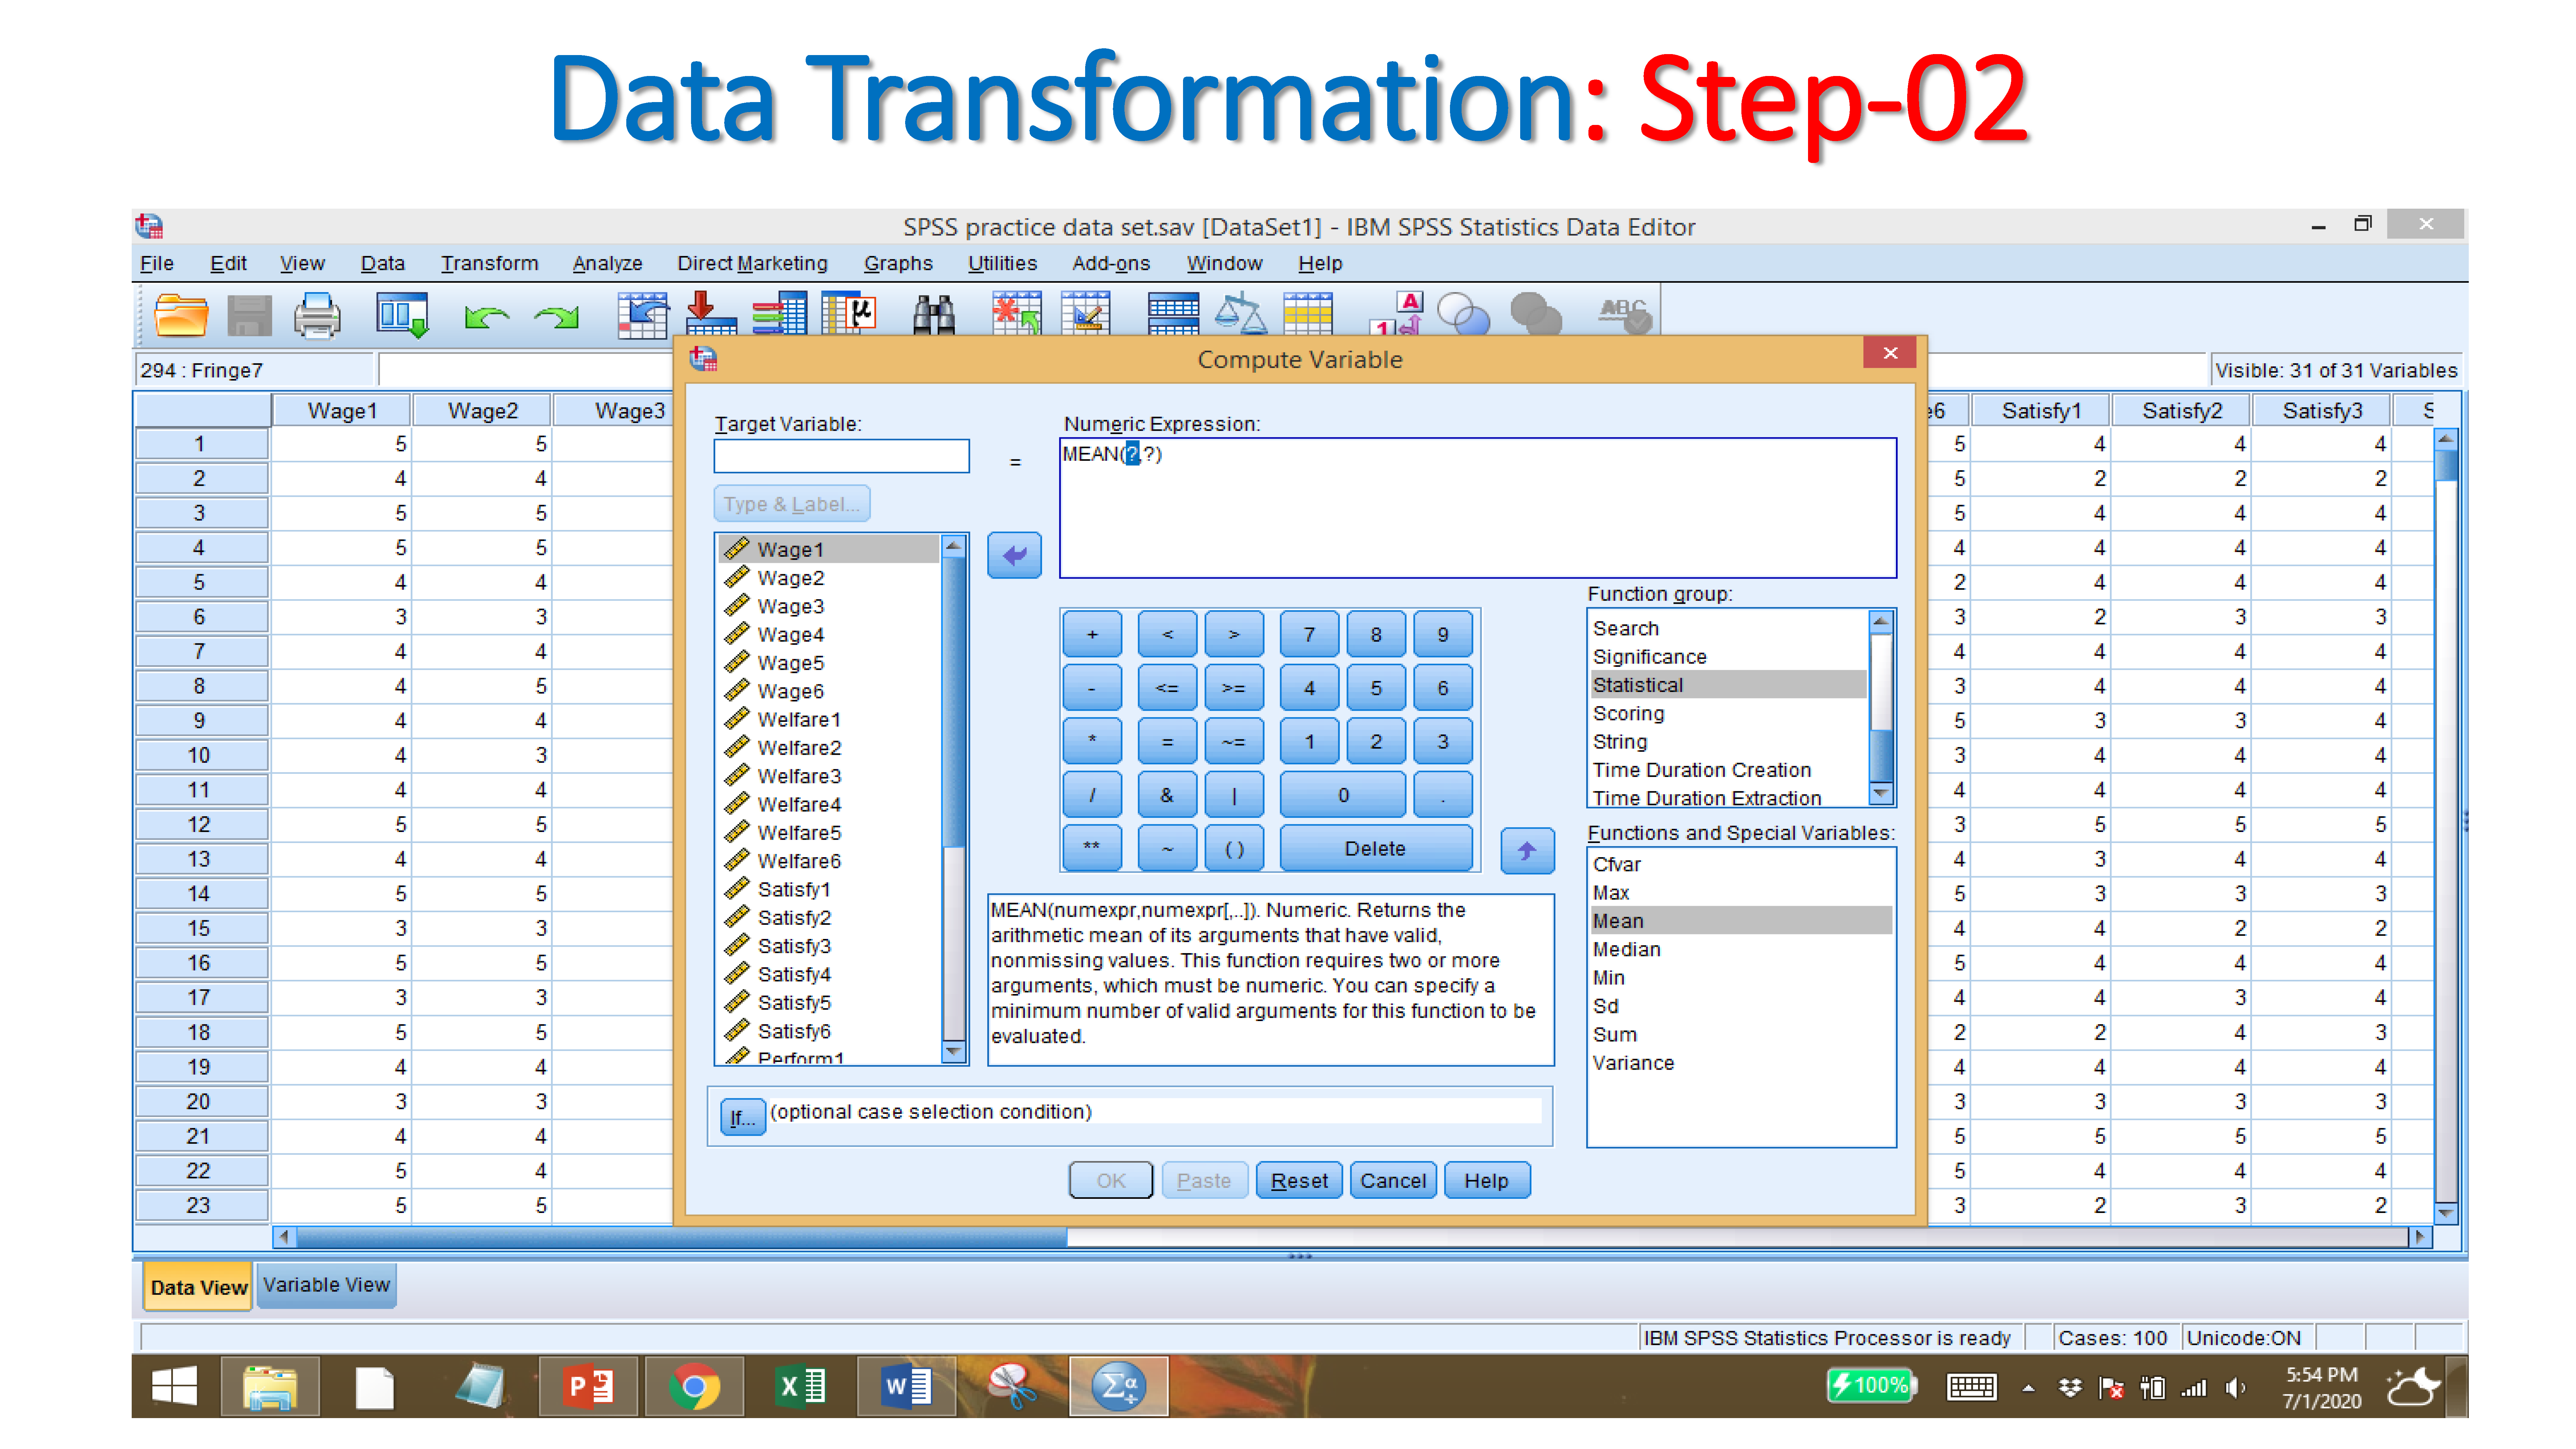
\includegraphics{images/slides/img_Page_017.png}

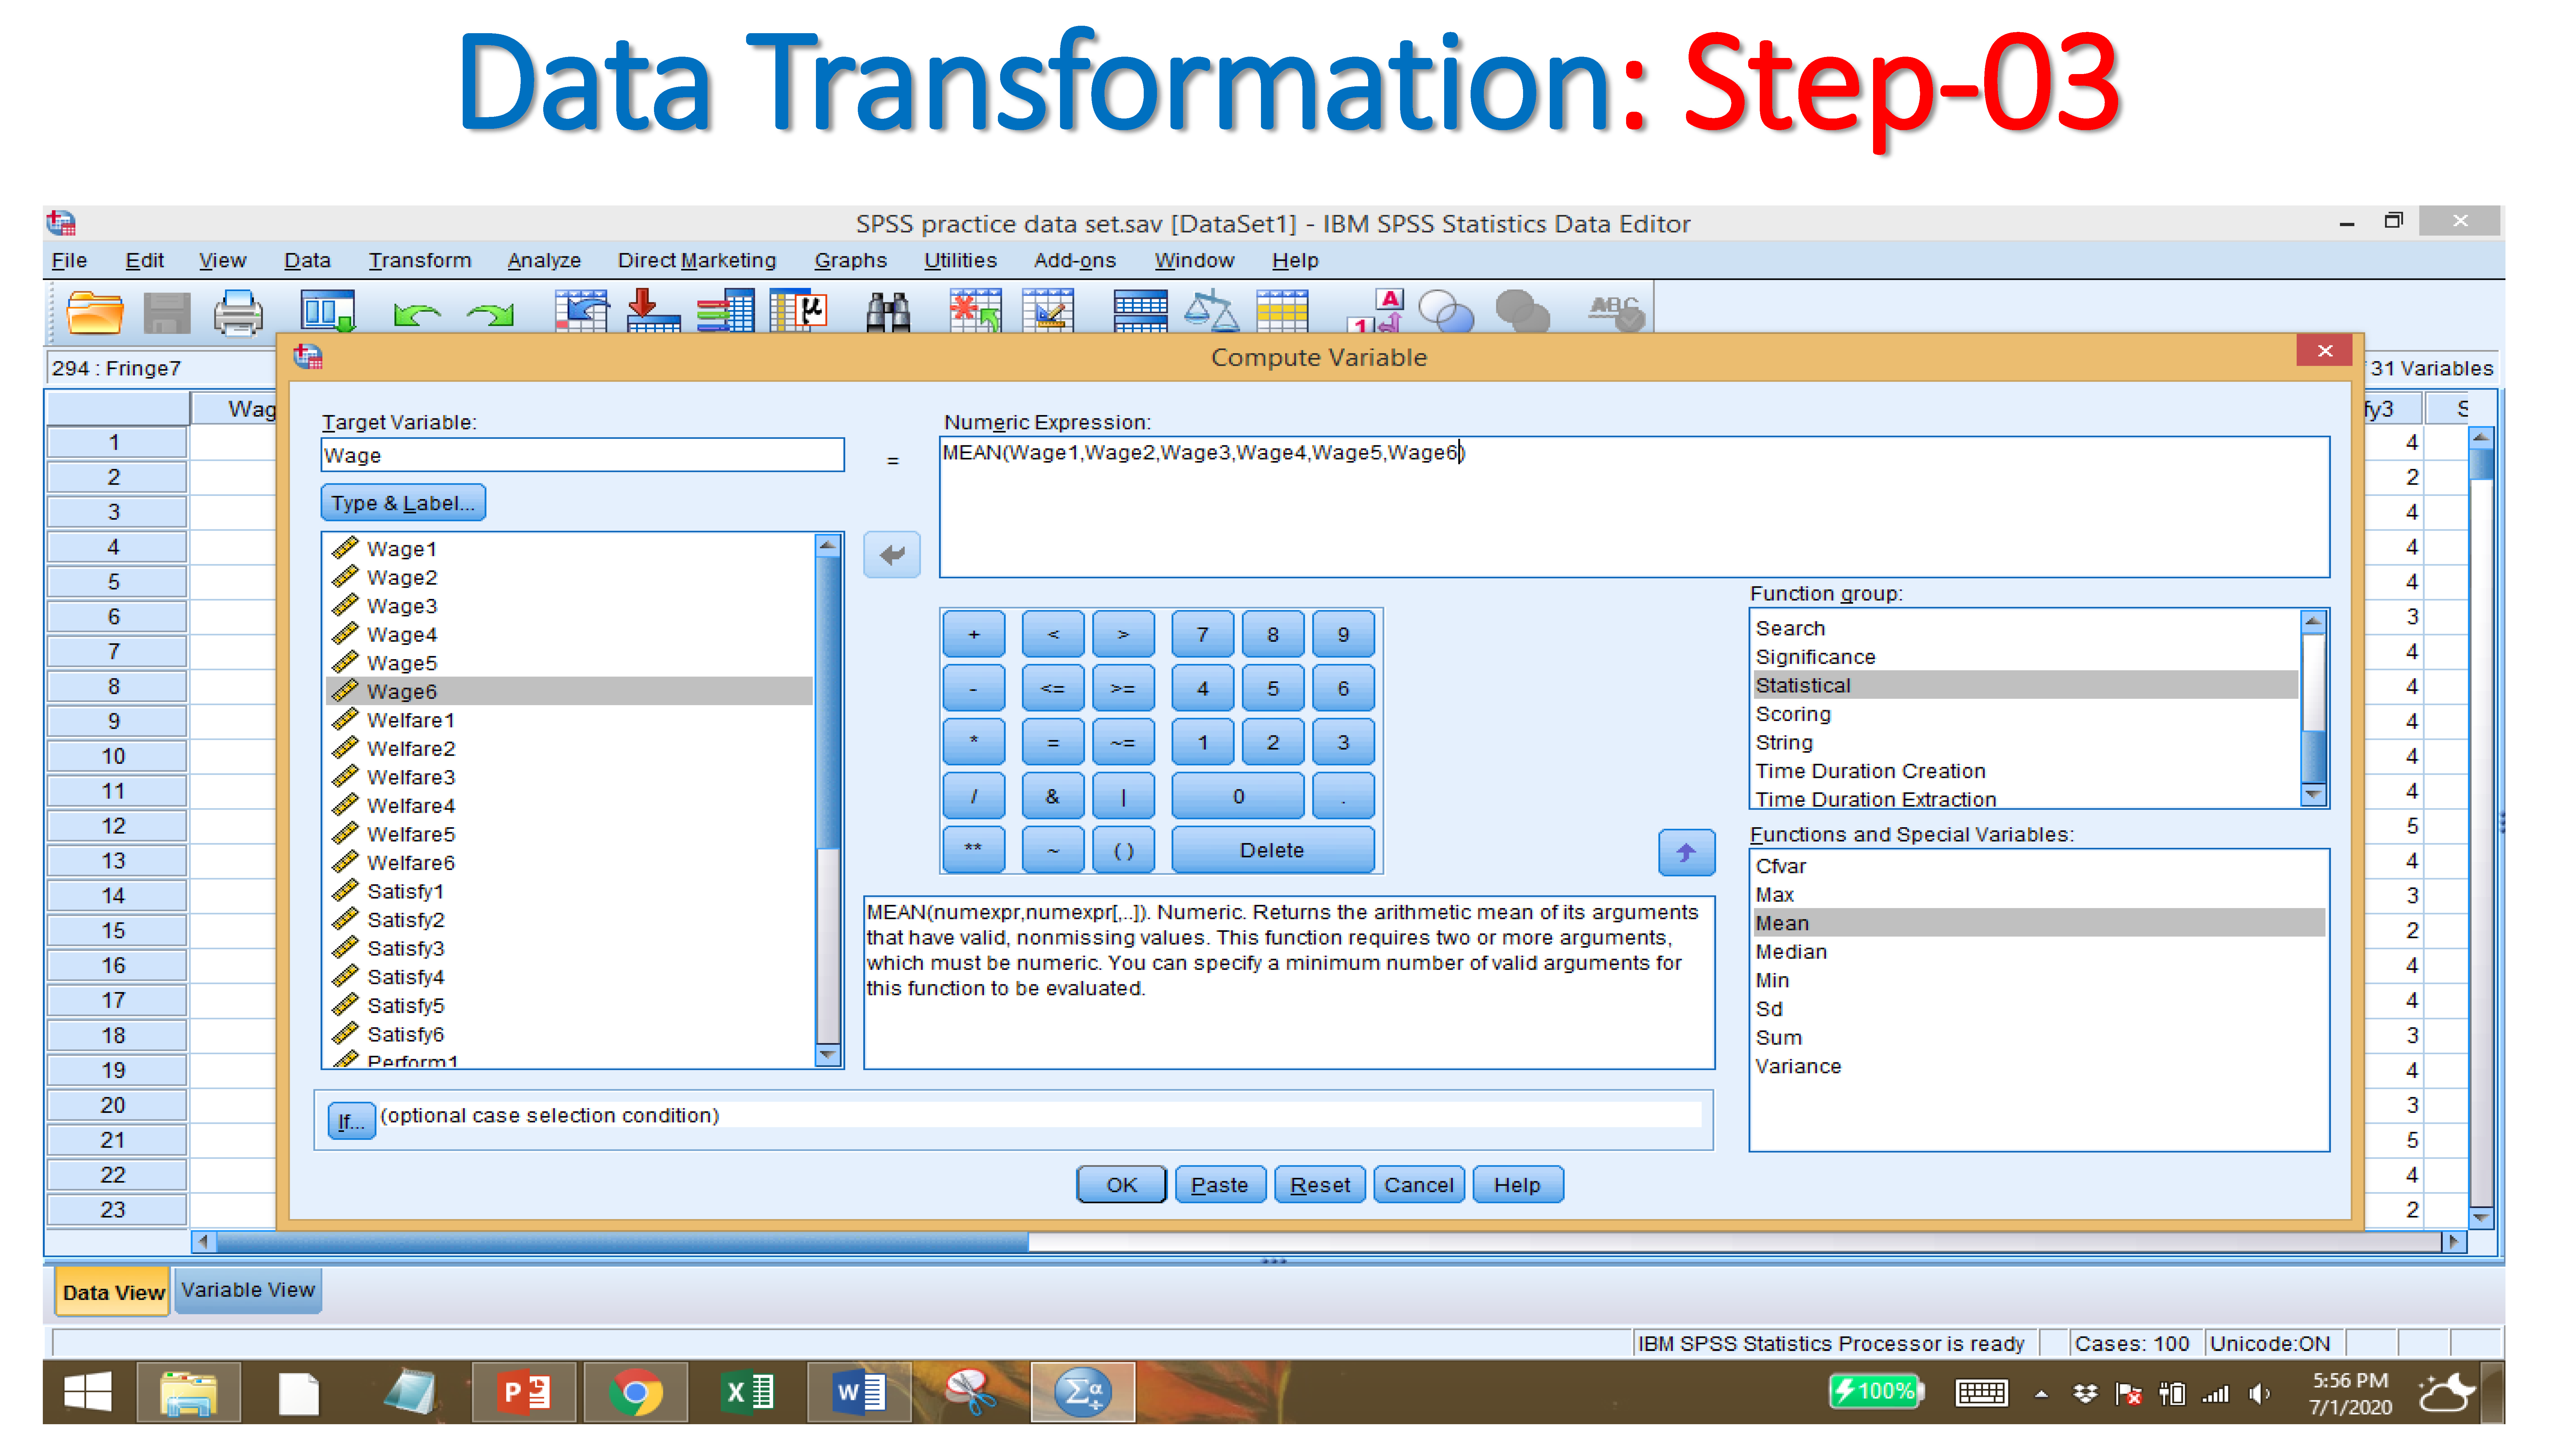
\includegraphics{images/slides/img_Page_018.png}

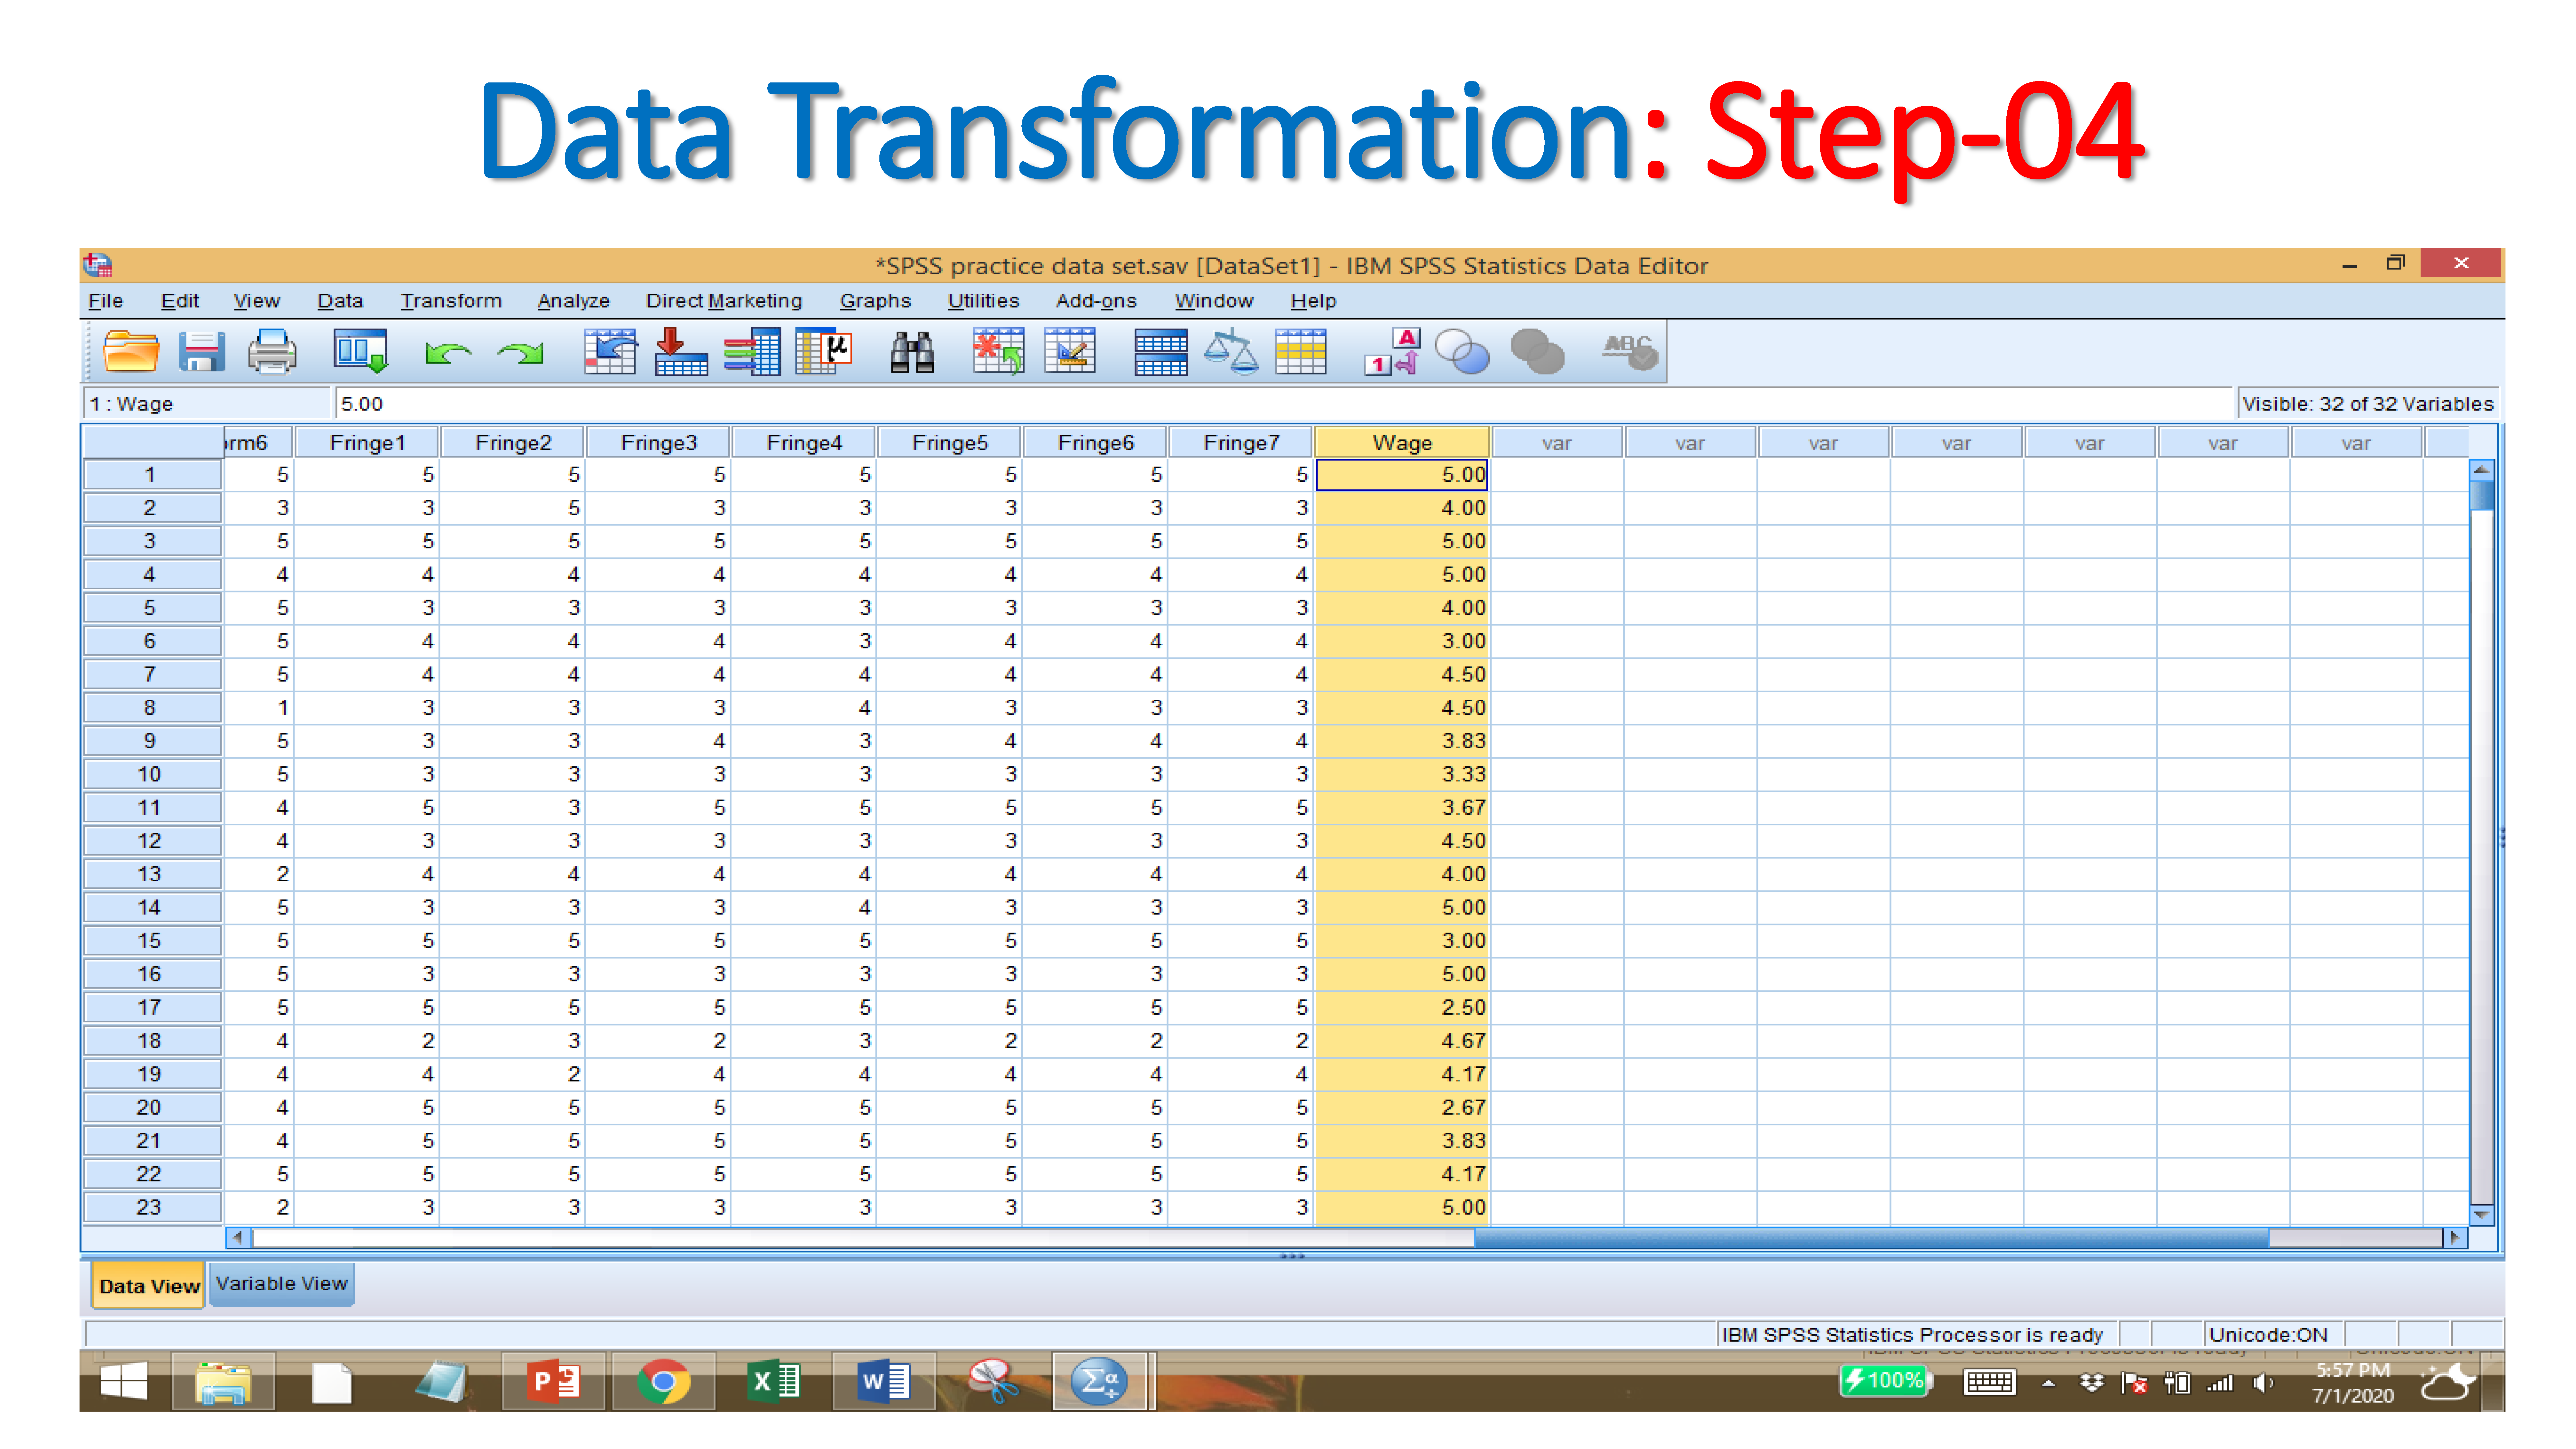
\includegraphics{images/slides/img_Page_019.png}

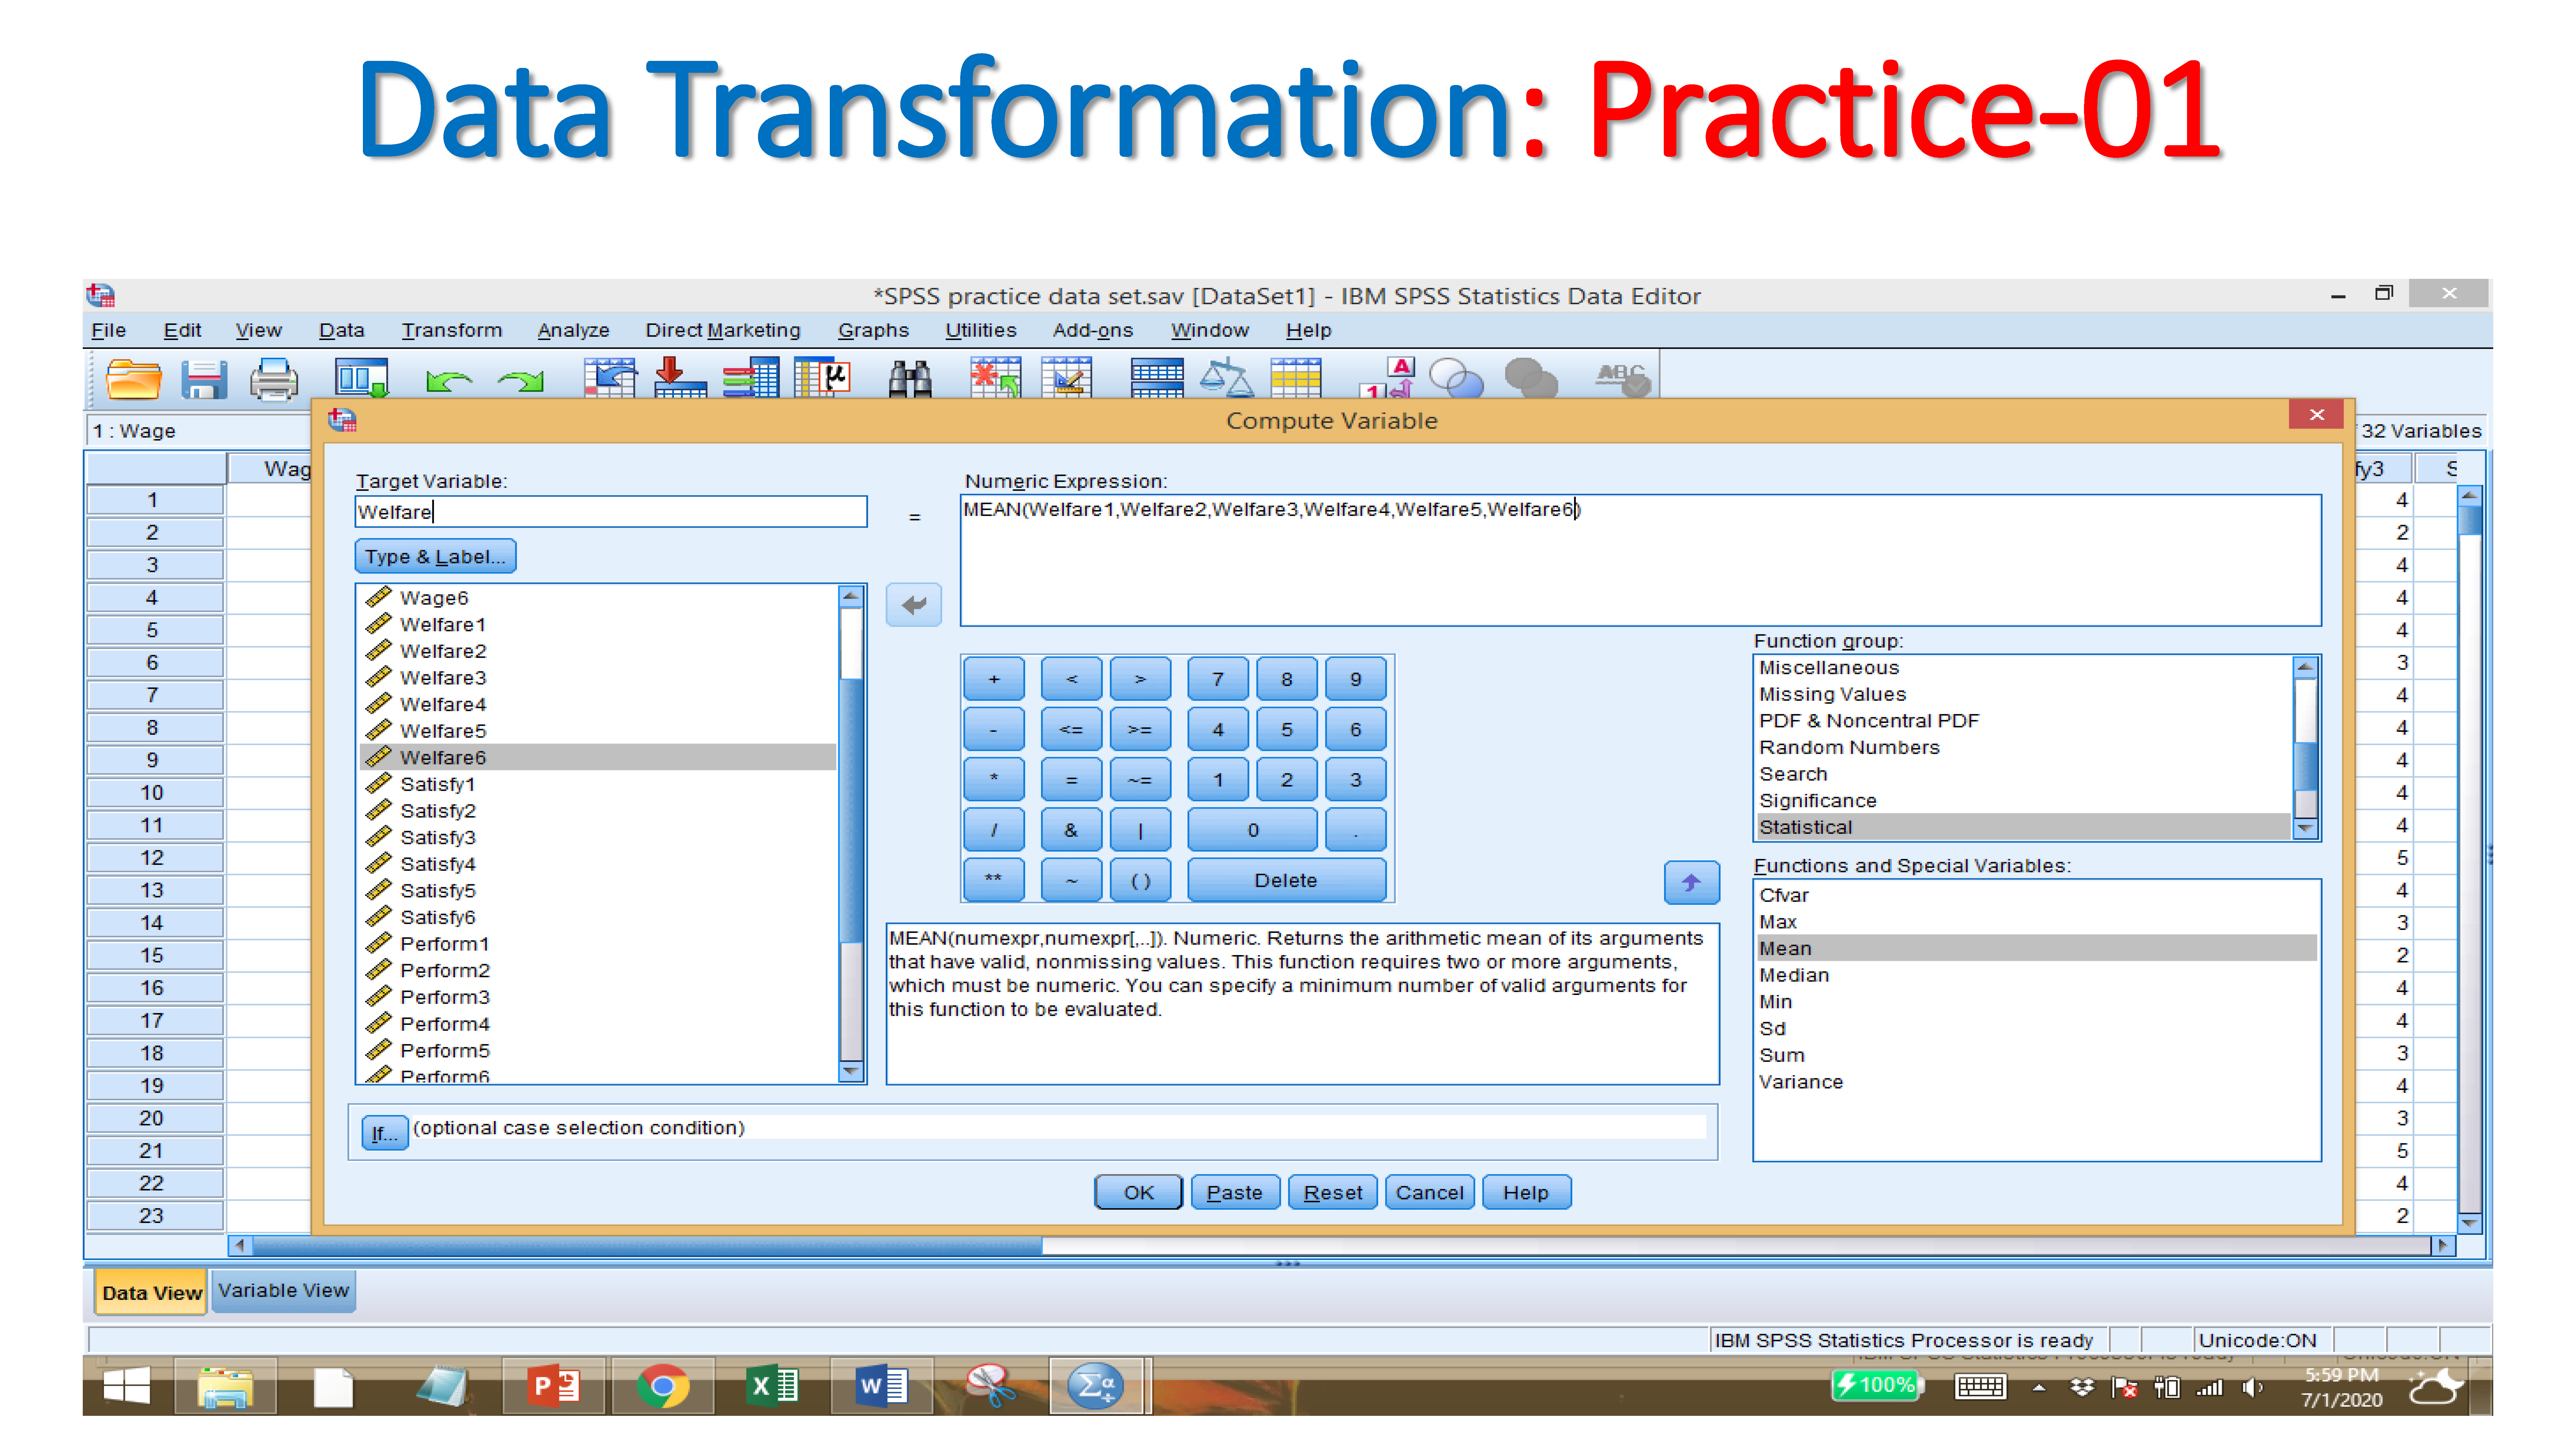
\includegraphics{images/slides/img_Page_020.png}

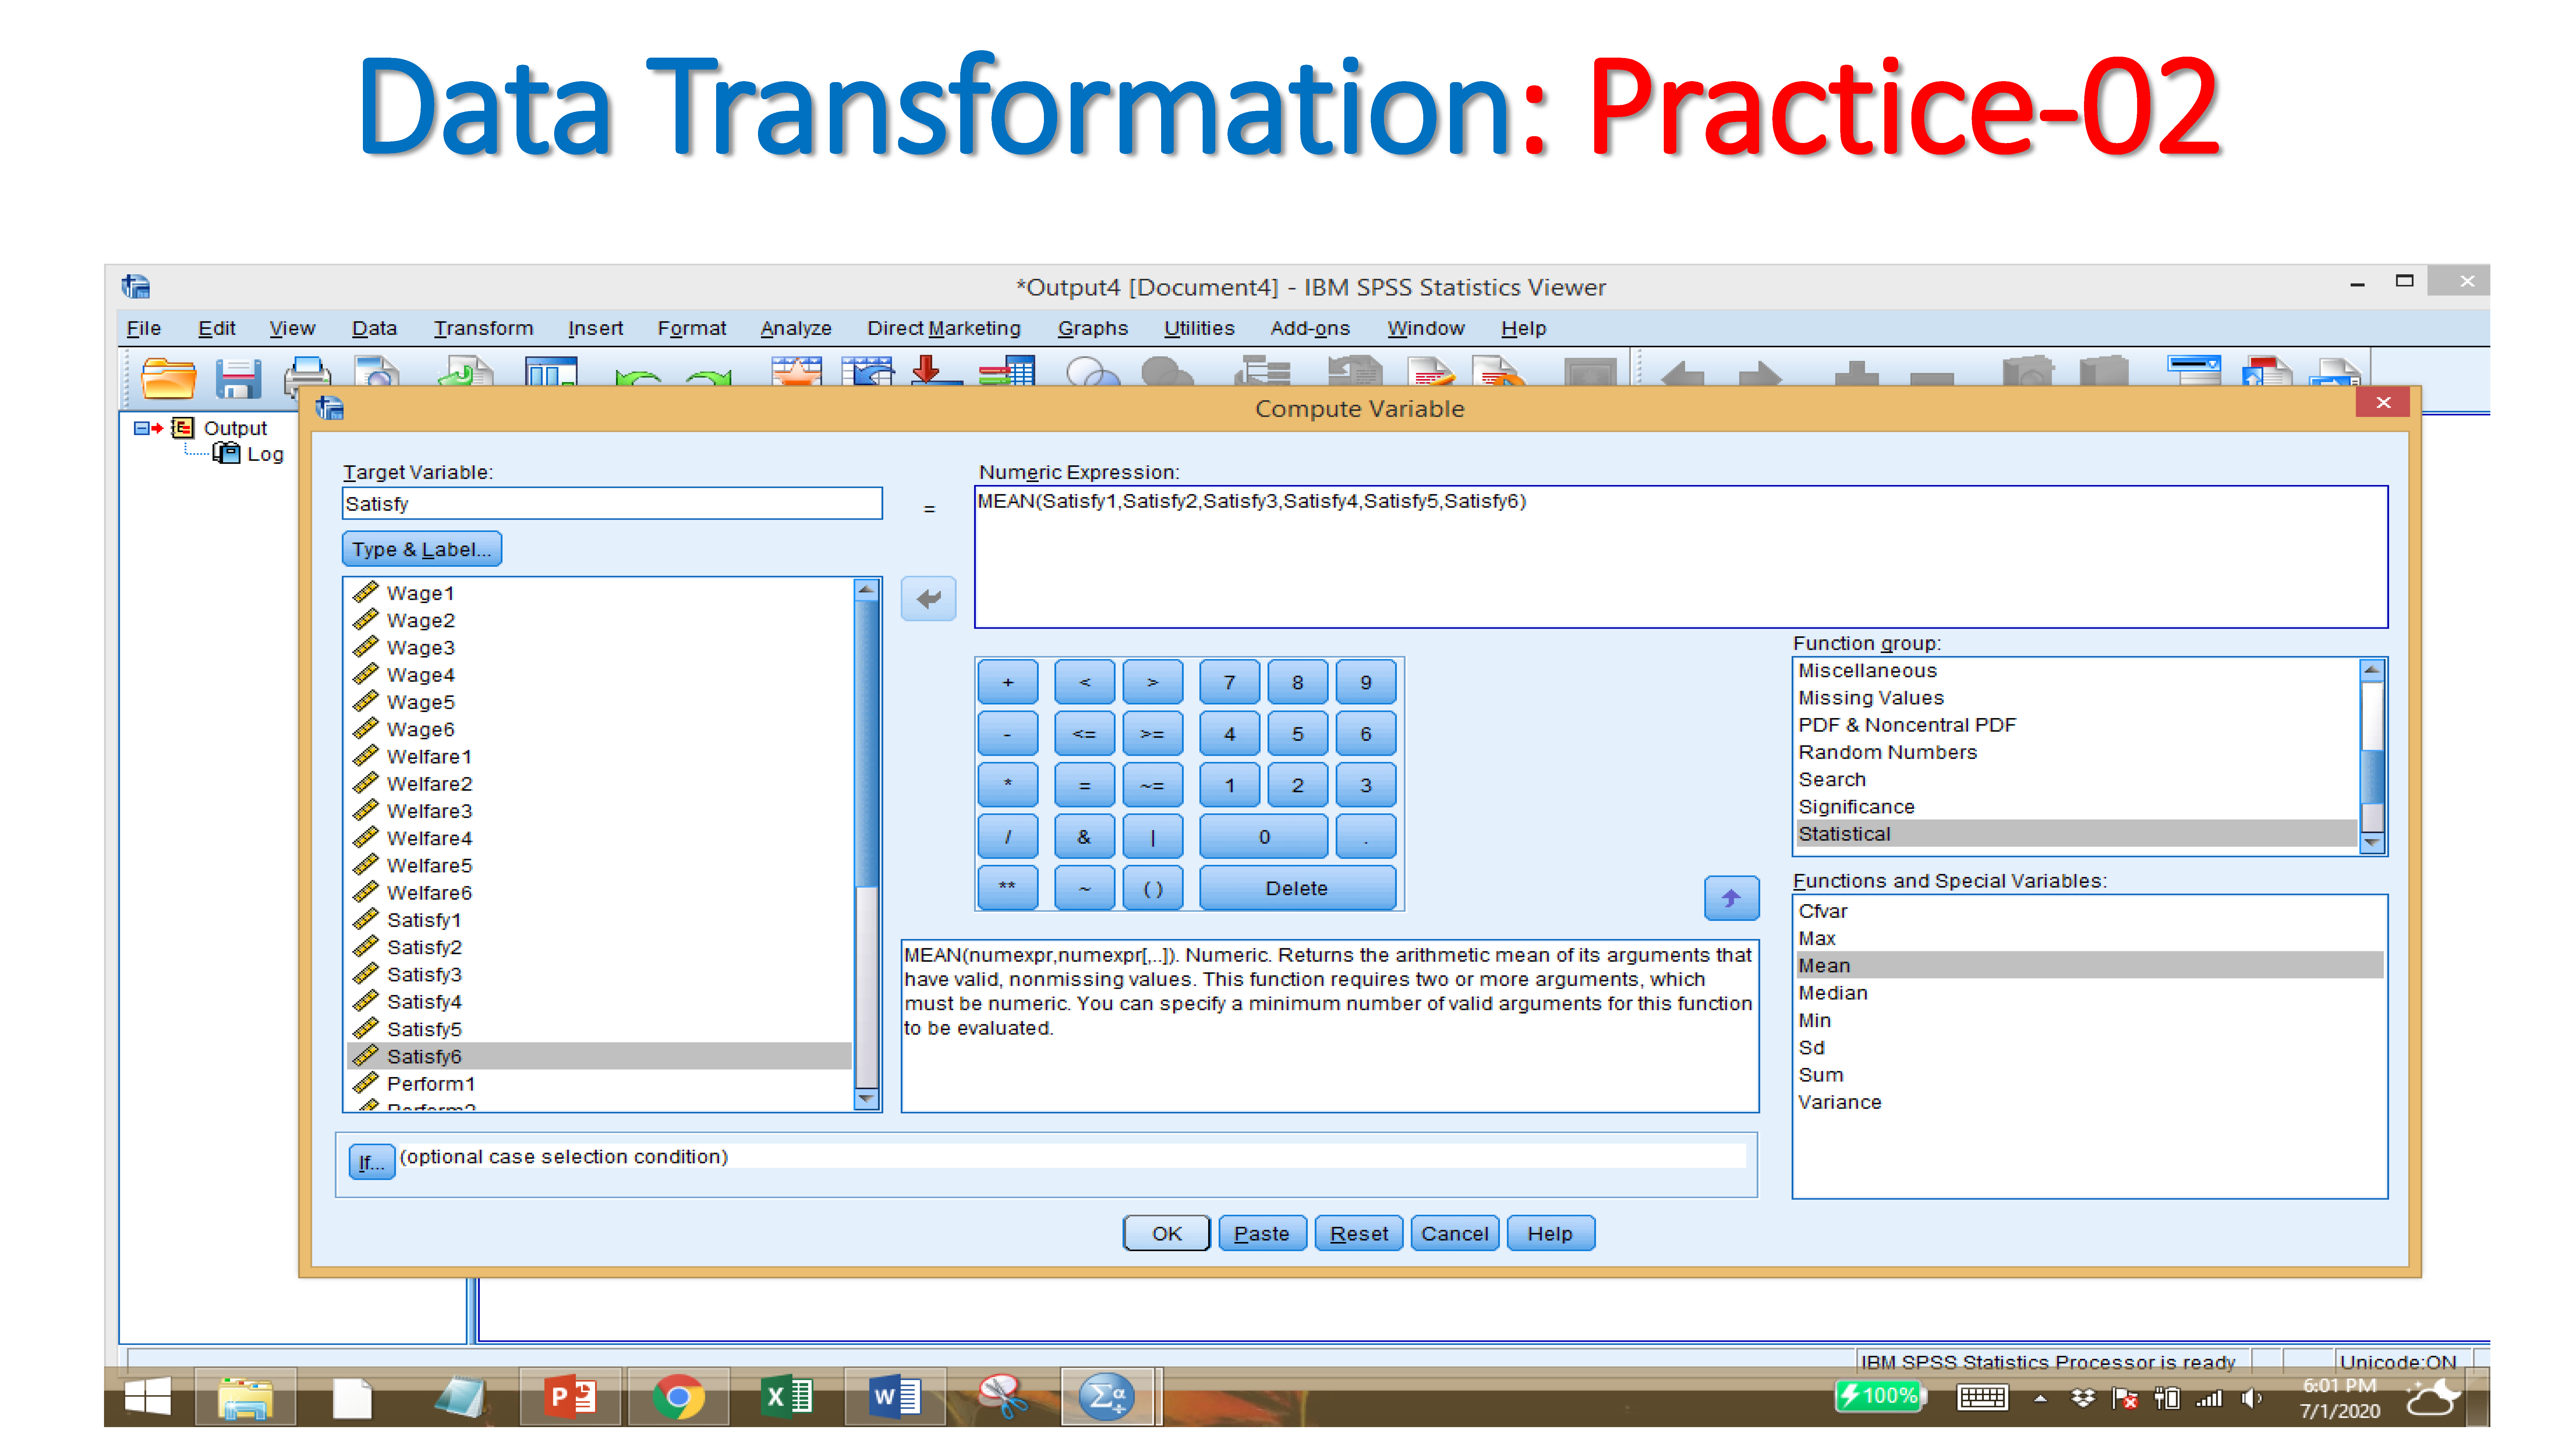
\includegraphics{images/slides/img_Page_021.png}

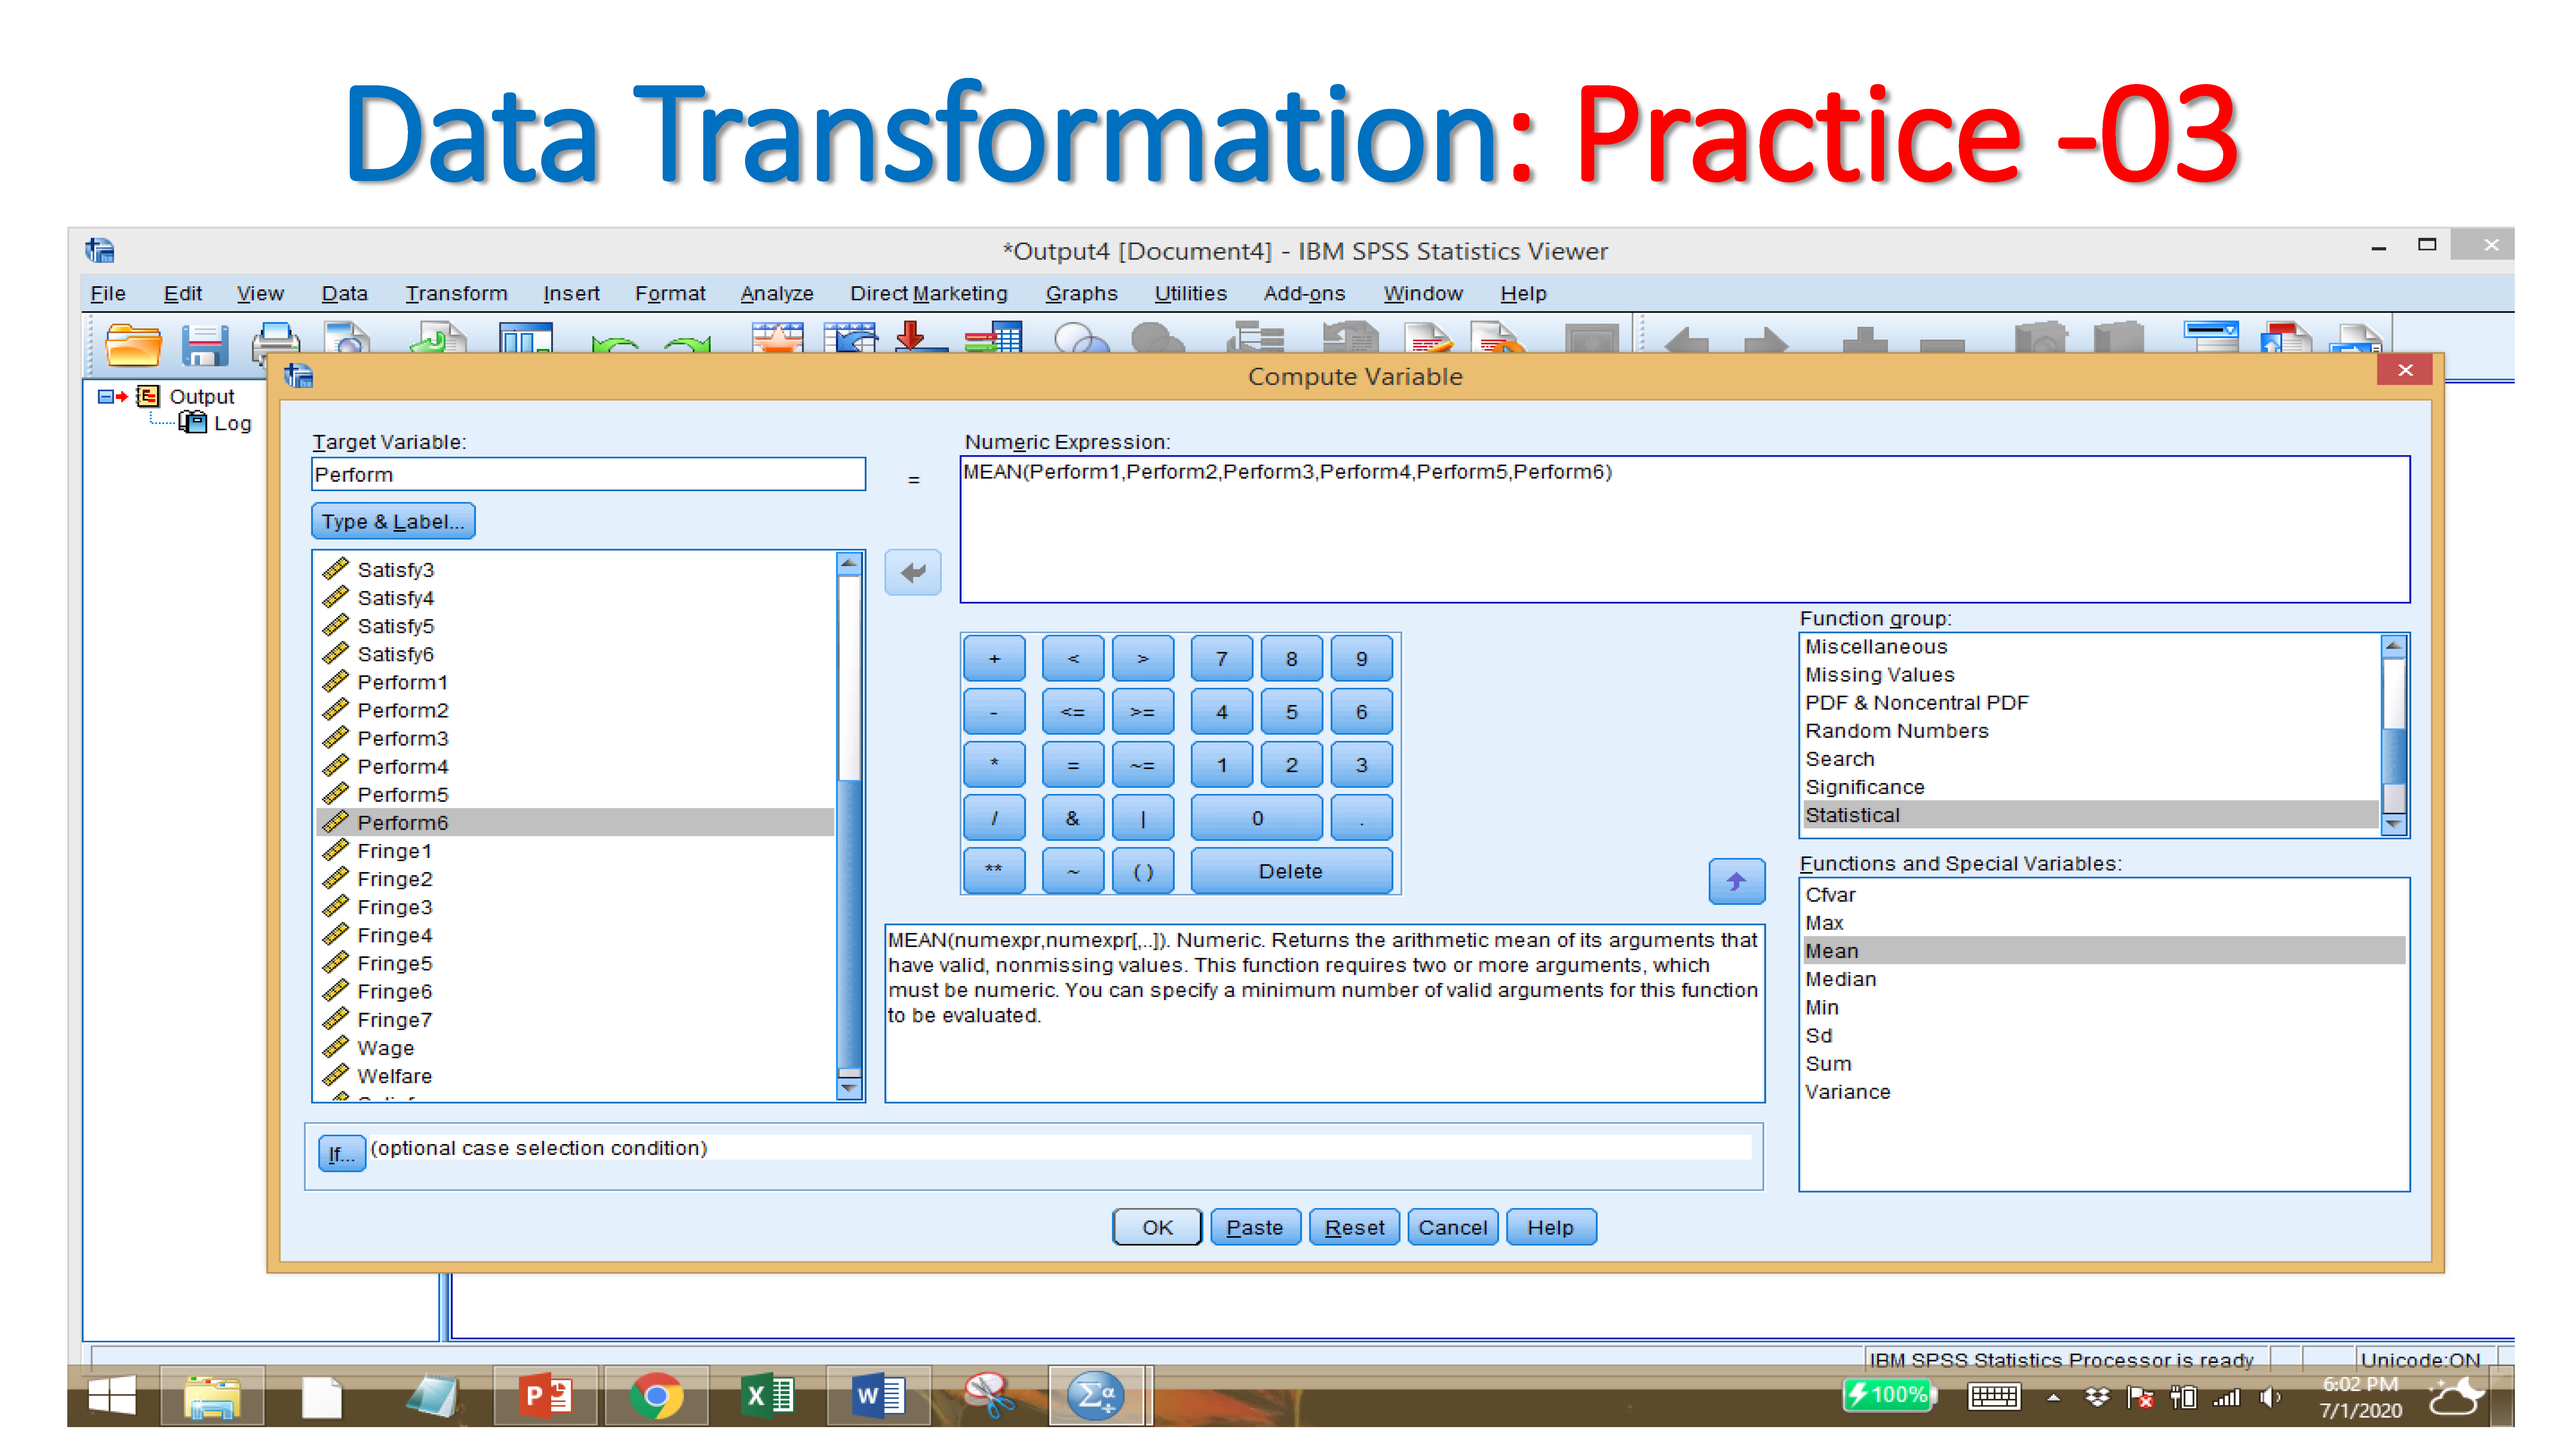
\includegraphics{images/slides/img_Page_022.png}

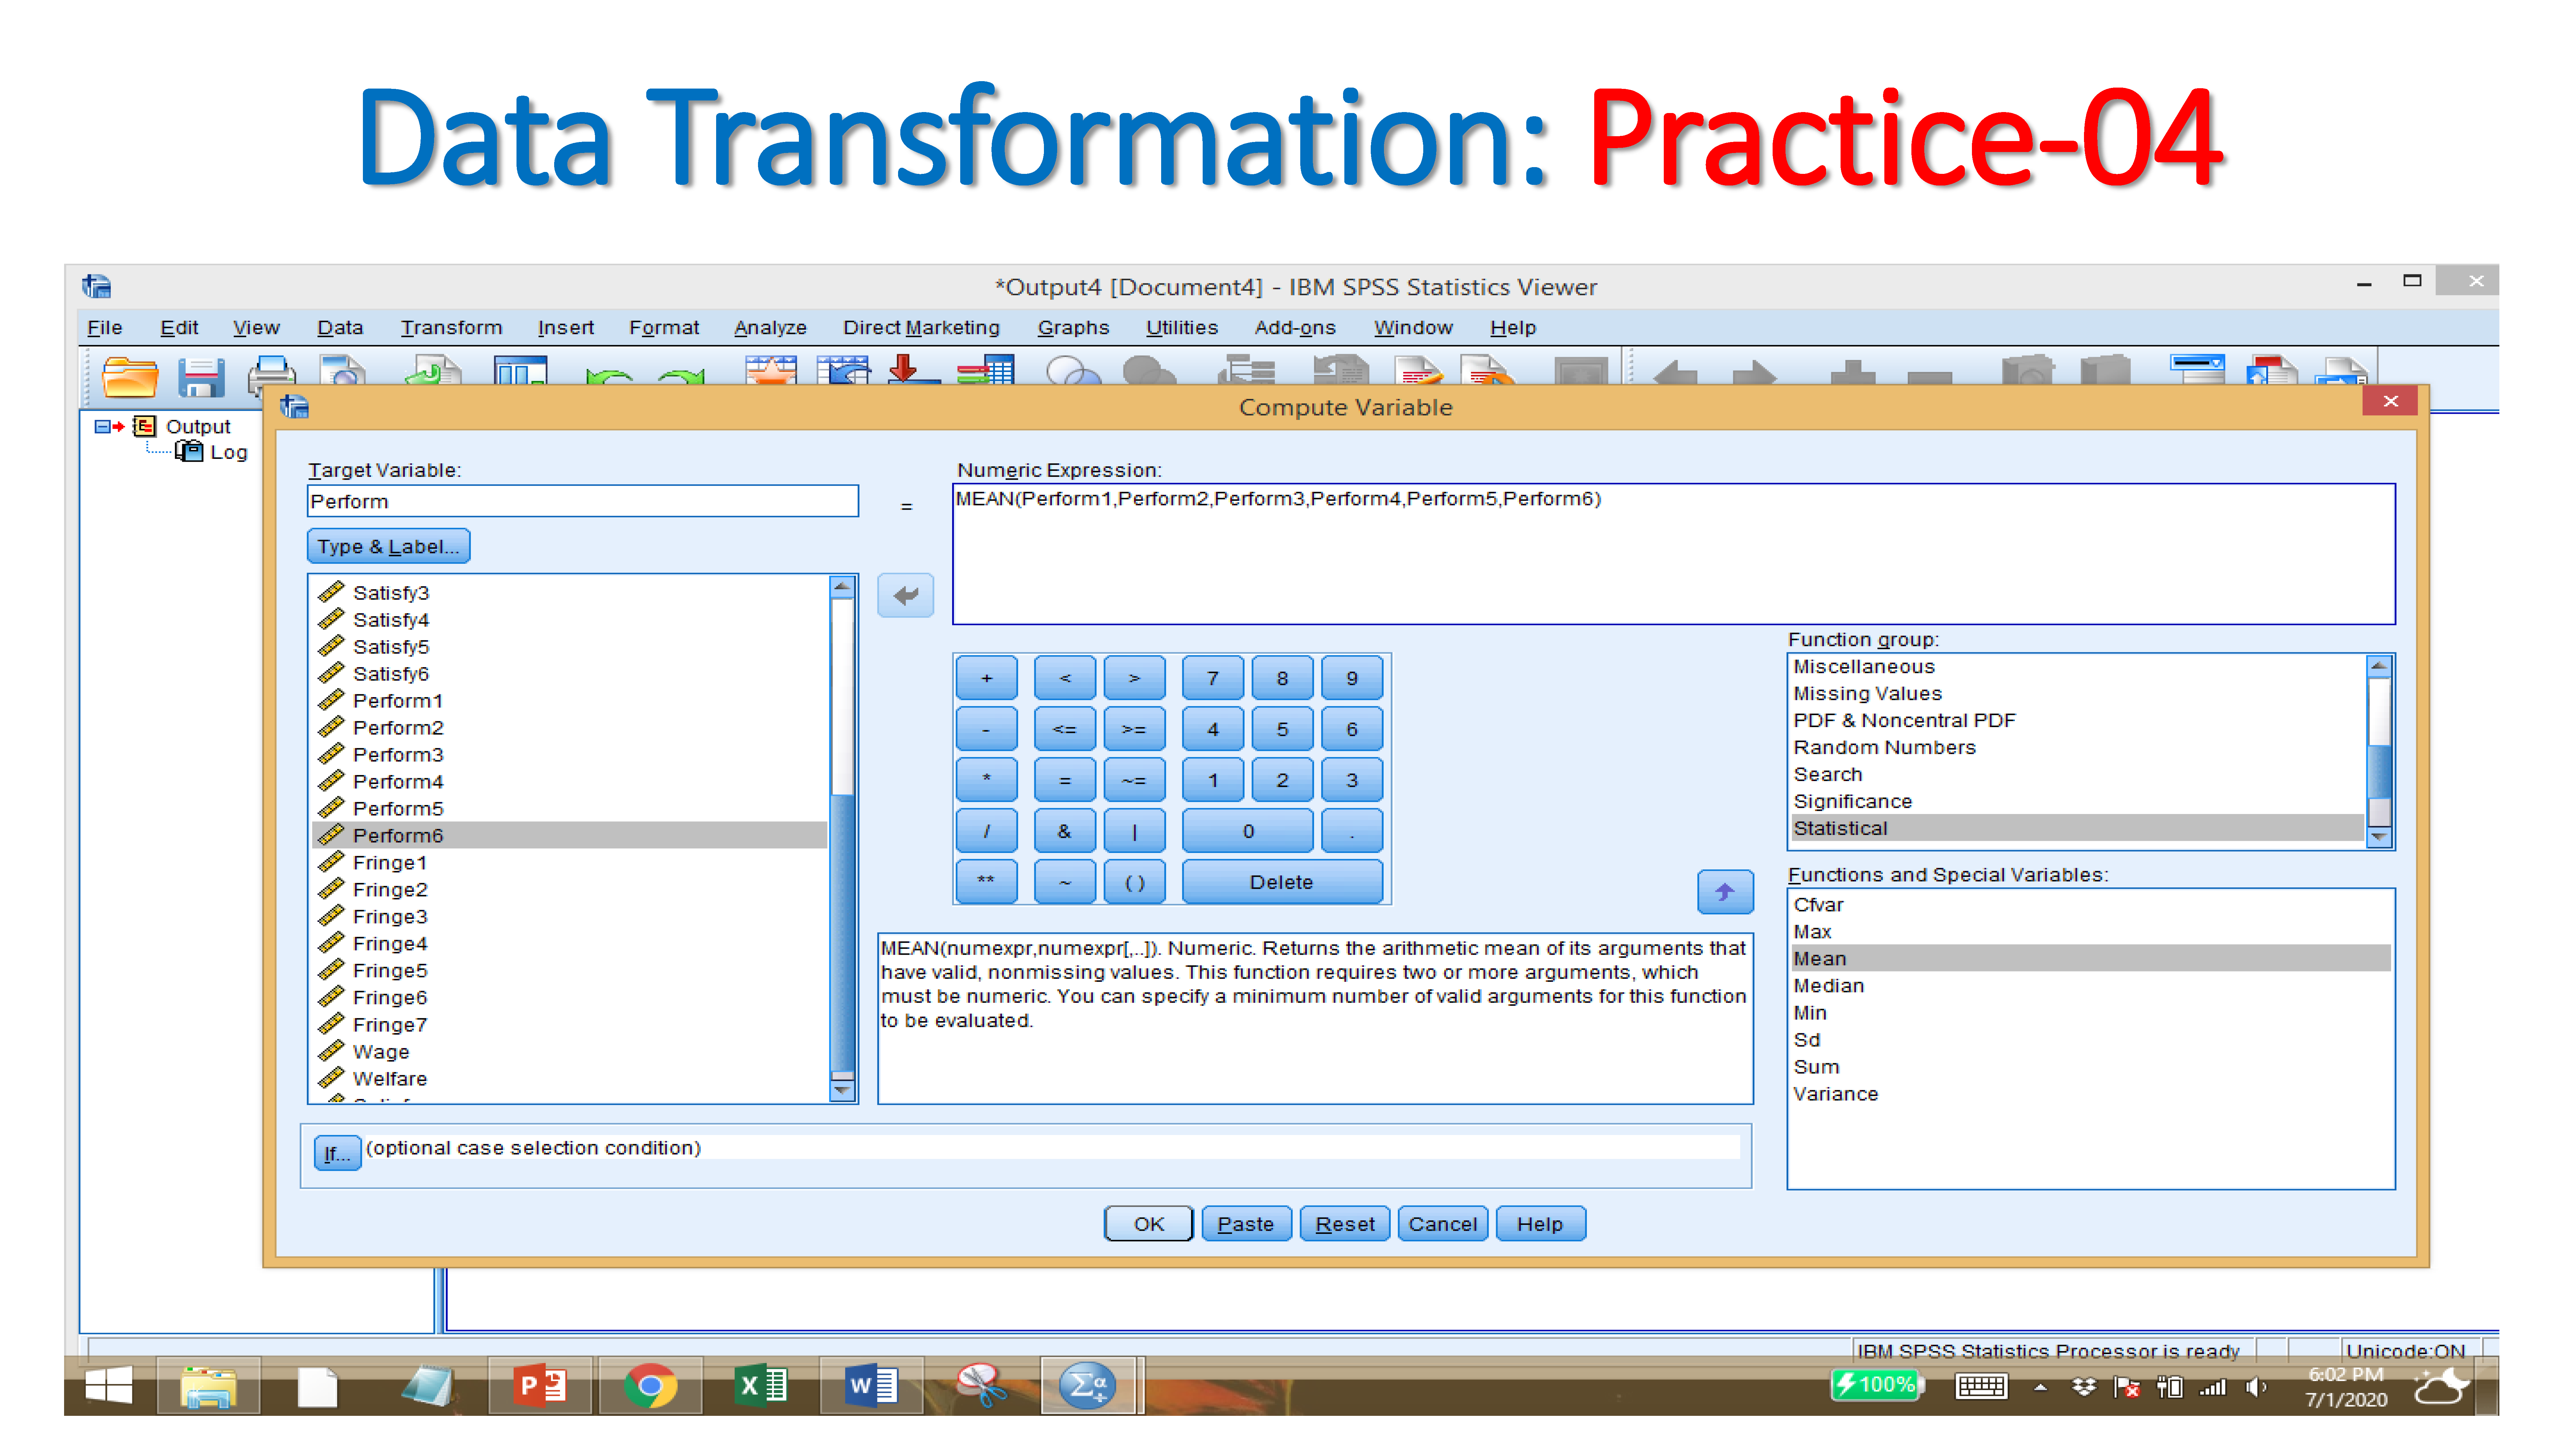
\includegraphics{images/slides/img_Page_023.png}

\bookmarksetup{startatroot}

\chapter{Descriptive Statistics}\label{descriptive-statistics}

A descriptive statistic is a summary statistic that quantitatively
describes or summarizes features of a collection of information, while
descriptive statistics is the process of using and analyzing those
statistics.\\

\section{Frequency Analysis}\label{frequency-analysis}

After Importing your data set, and providing names to variables, click
on:\\

{ANALYZE → DESCRIPTIVE STATISTICS → FREQUENCIES}

Choose any variables to be analyzed and place them in box on right\\
Options include (For Categorical Variables):\\

\begin{itemize}
\tightlist
\item
  Frequency Tables\\
\item
  Pie Charts, Bar Charts\\
\end{itemize}

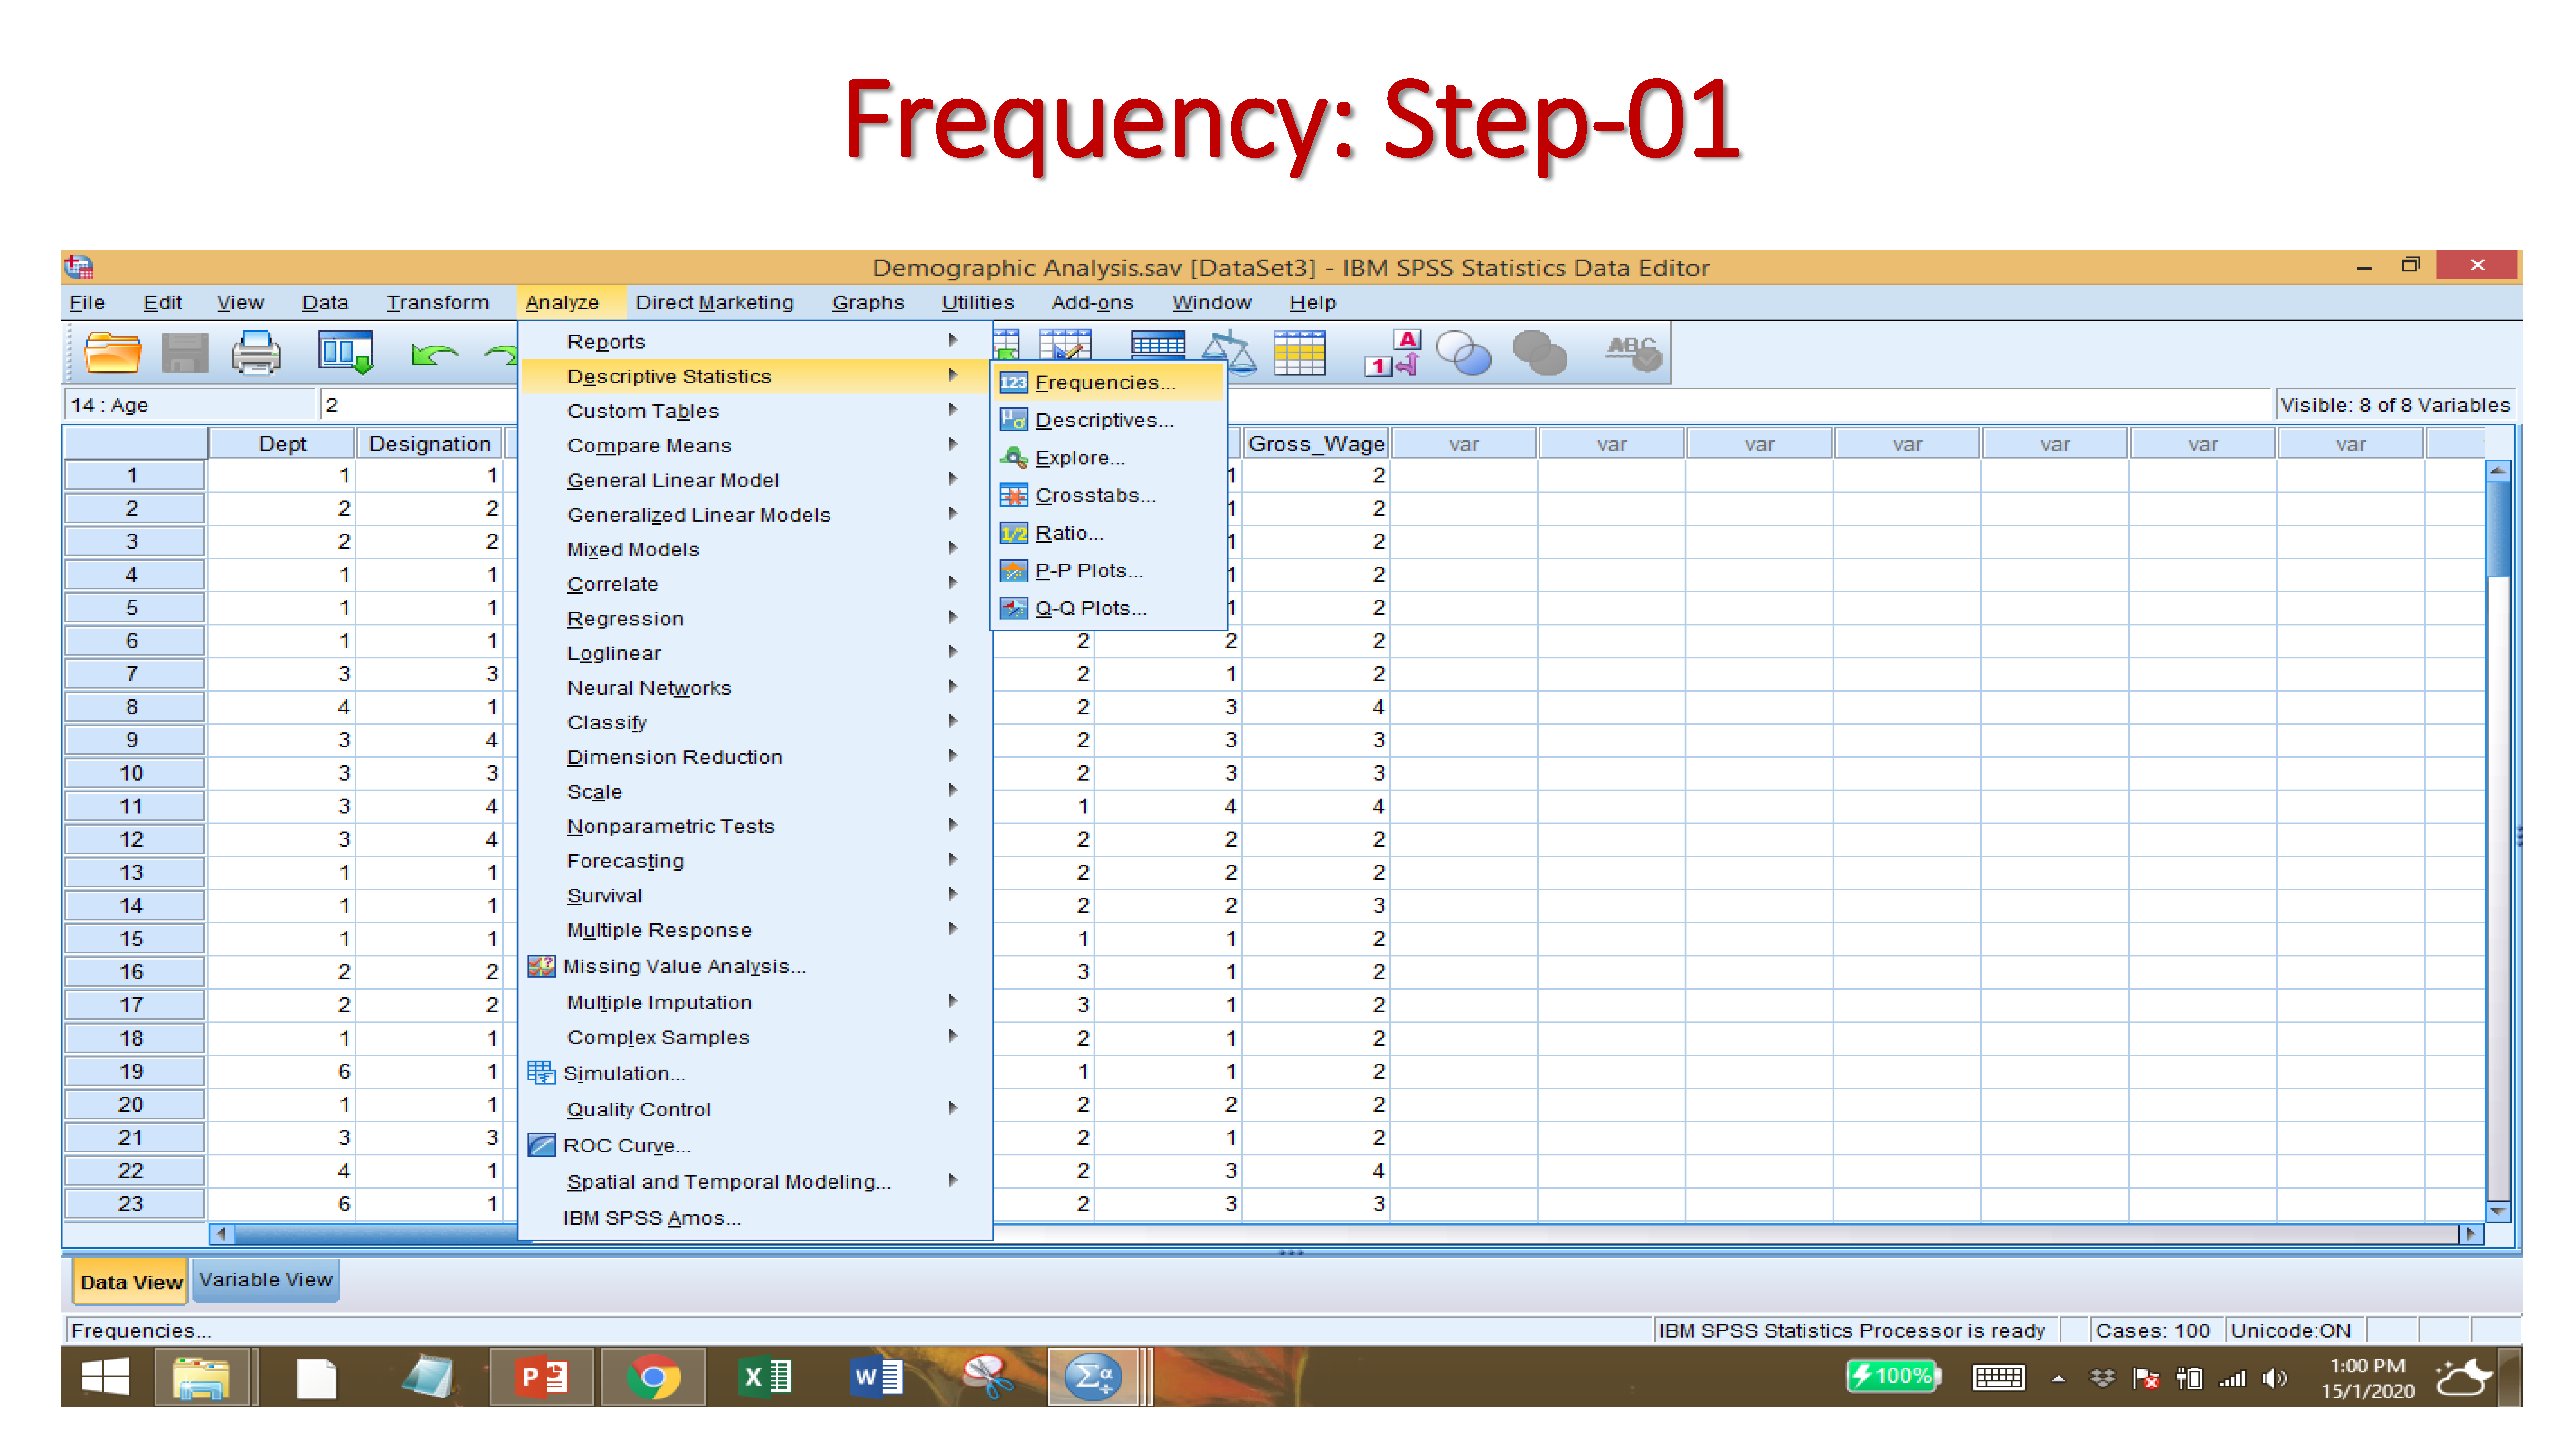
\includegraphics{images/slides/img_Page_026.png}

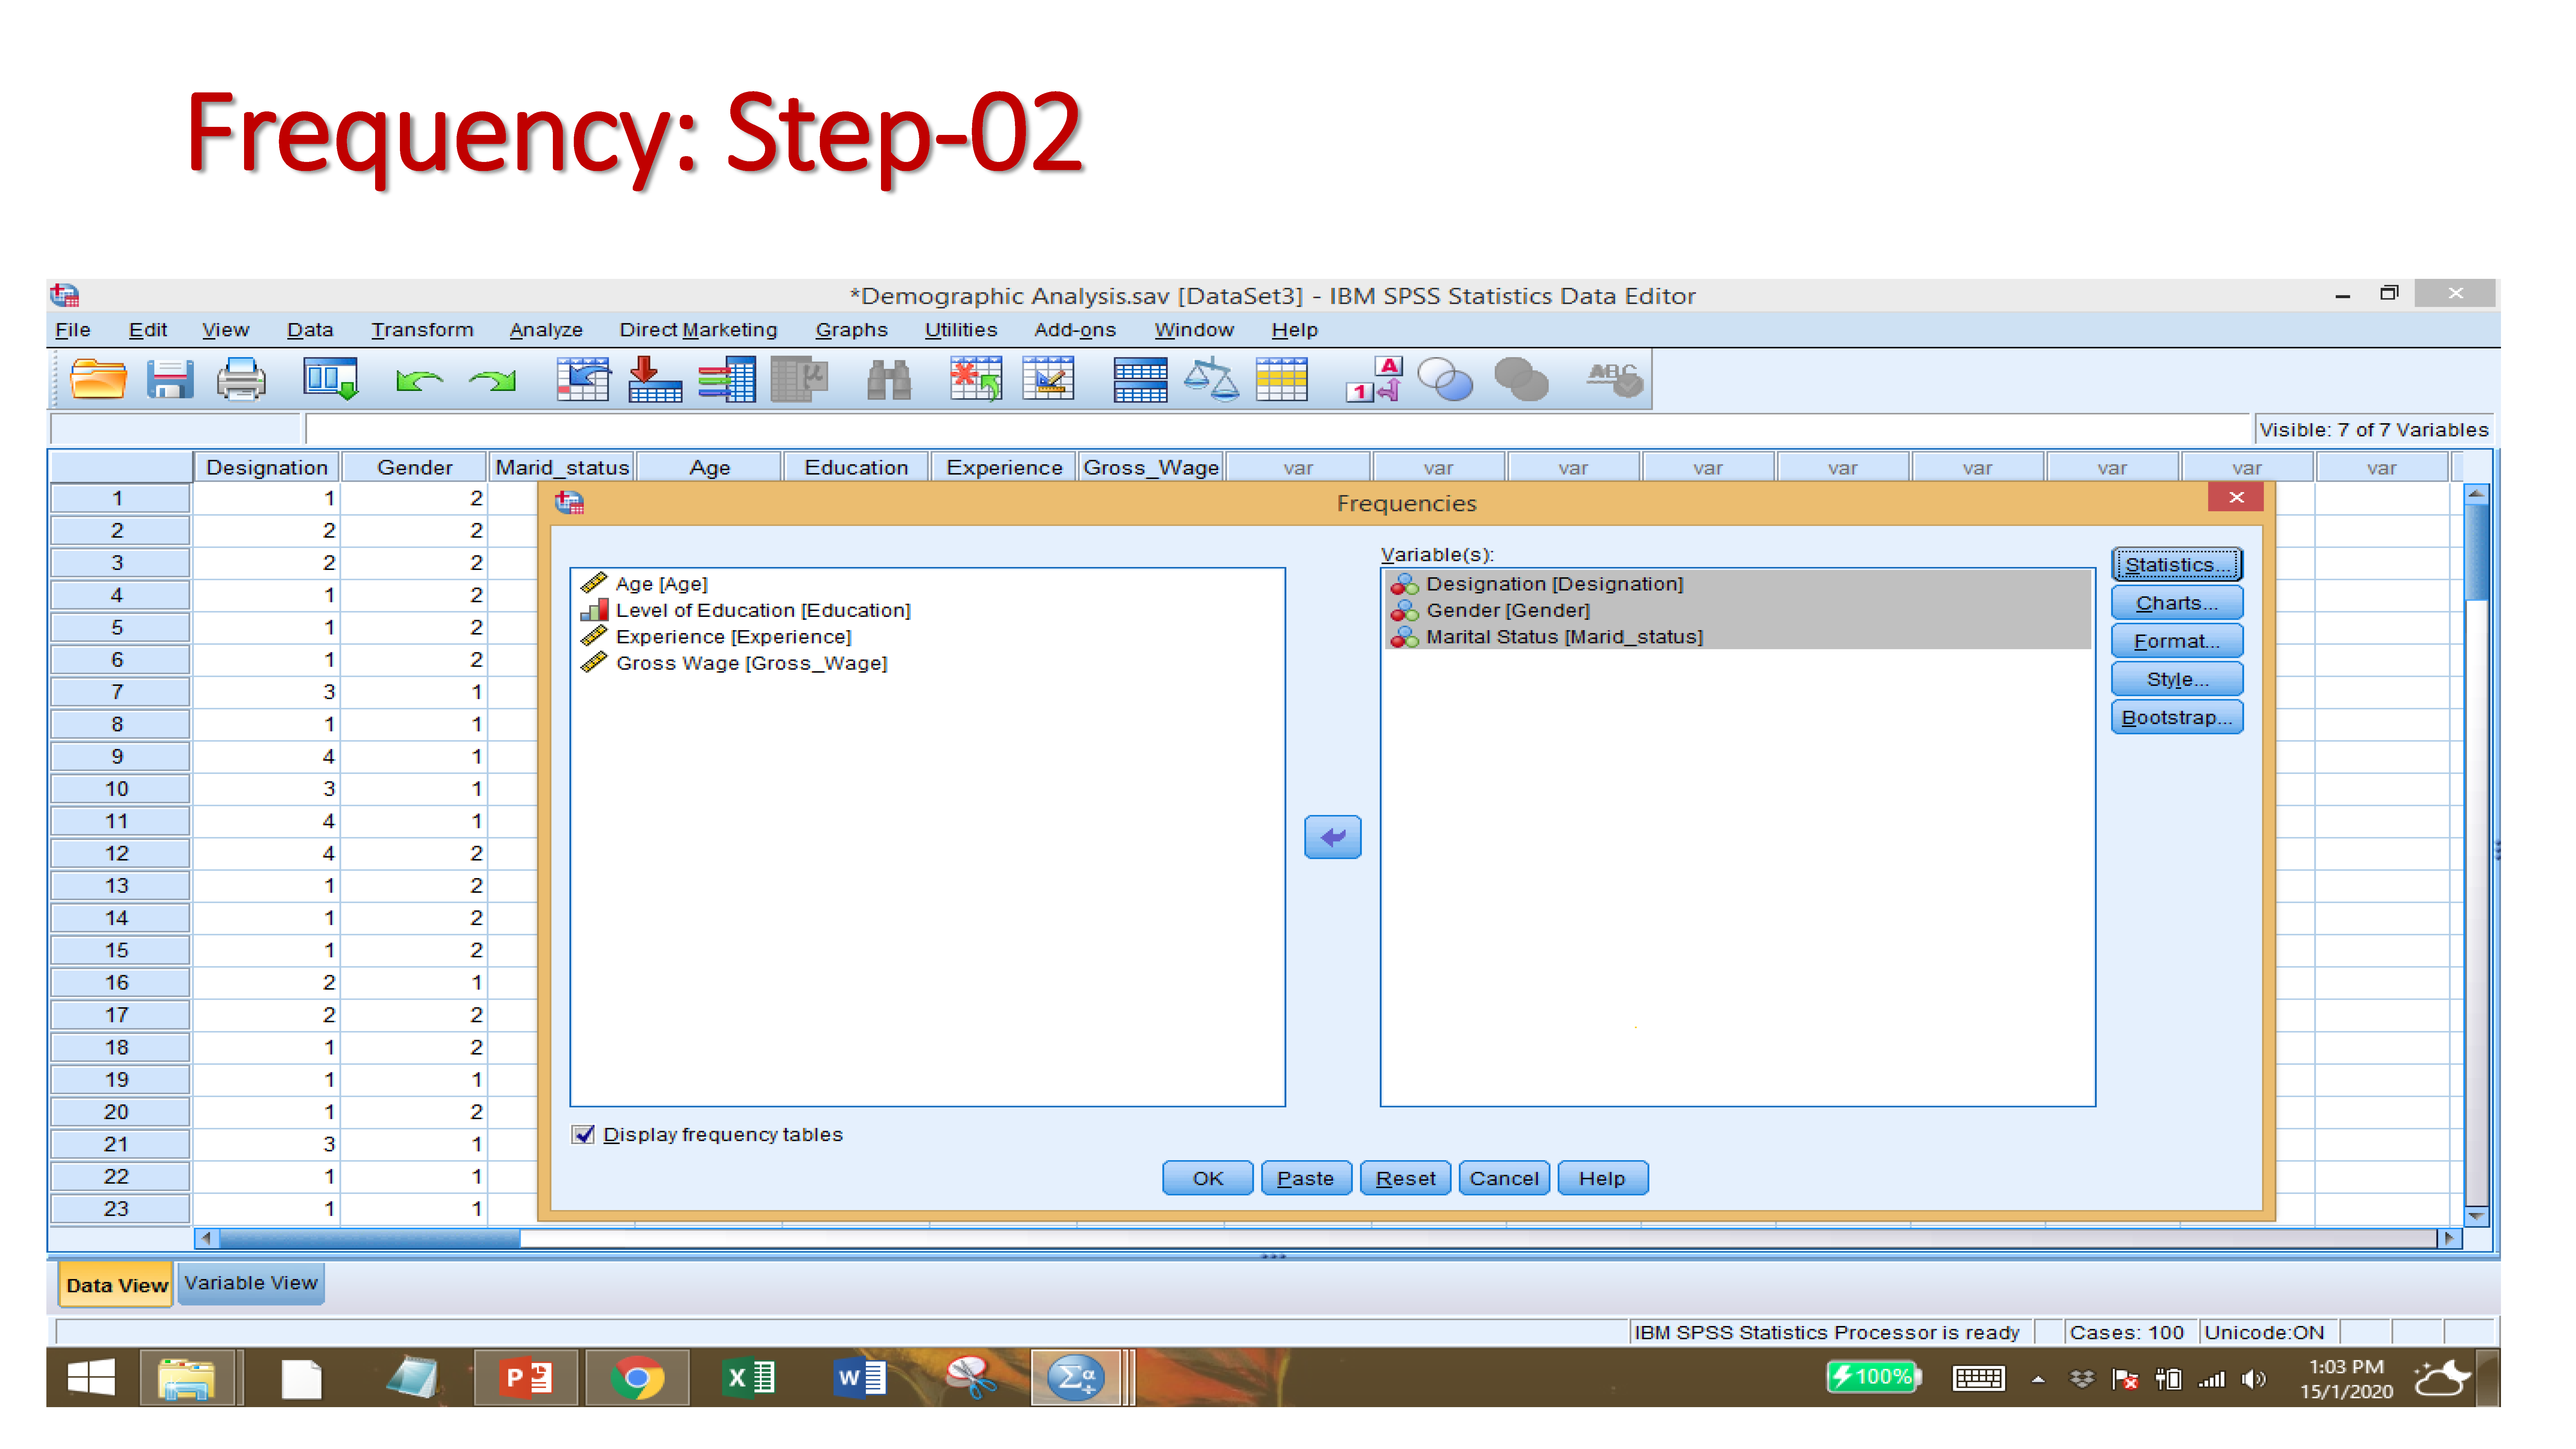
\includegraphics{images/slides/img_Page_027.png}

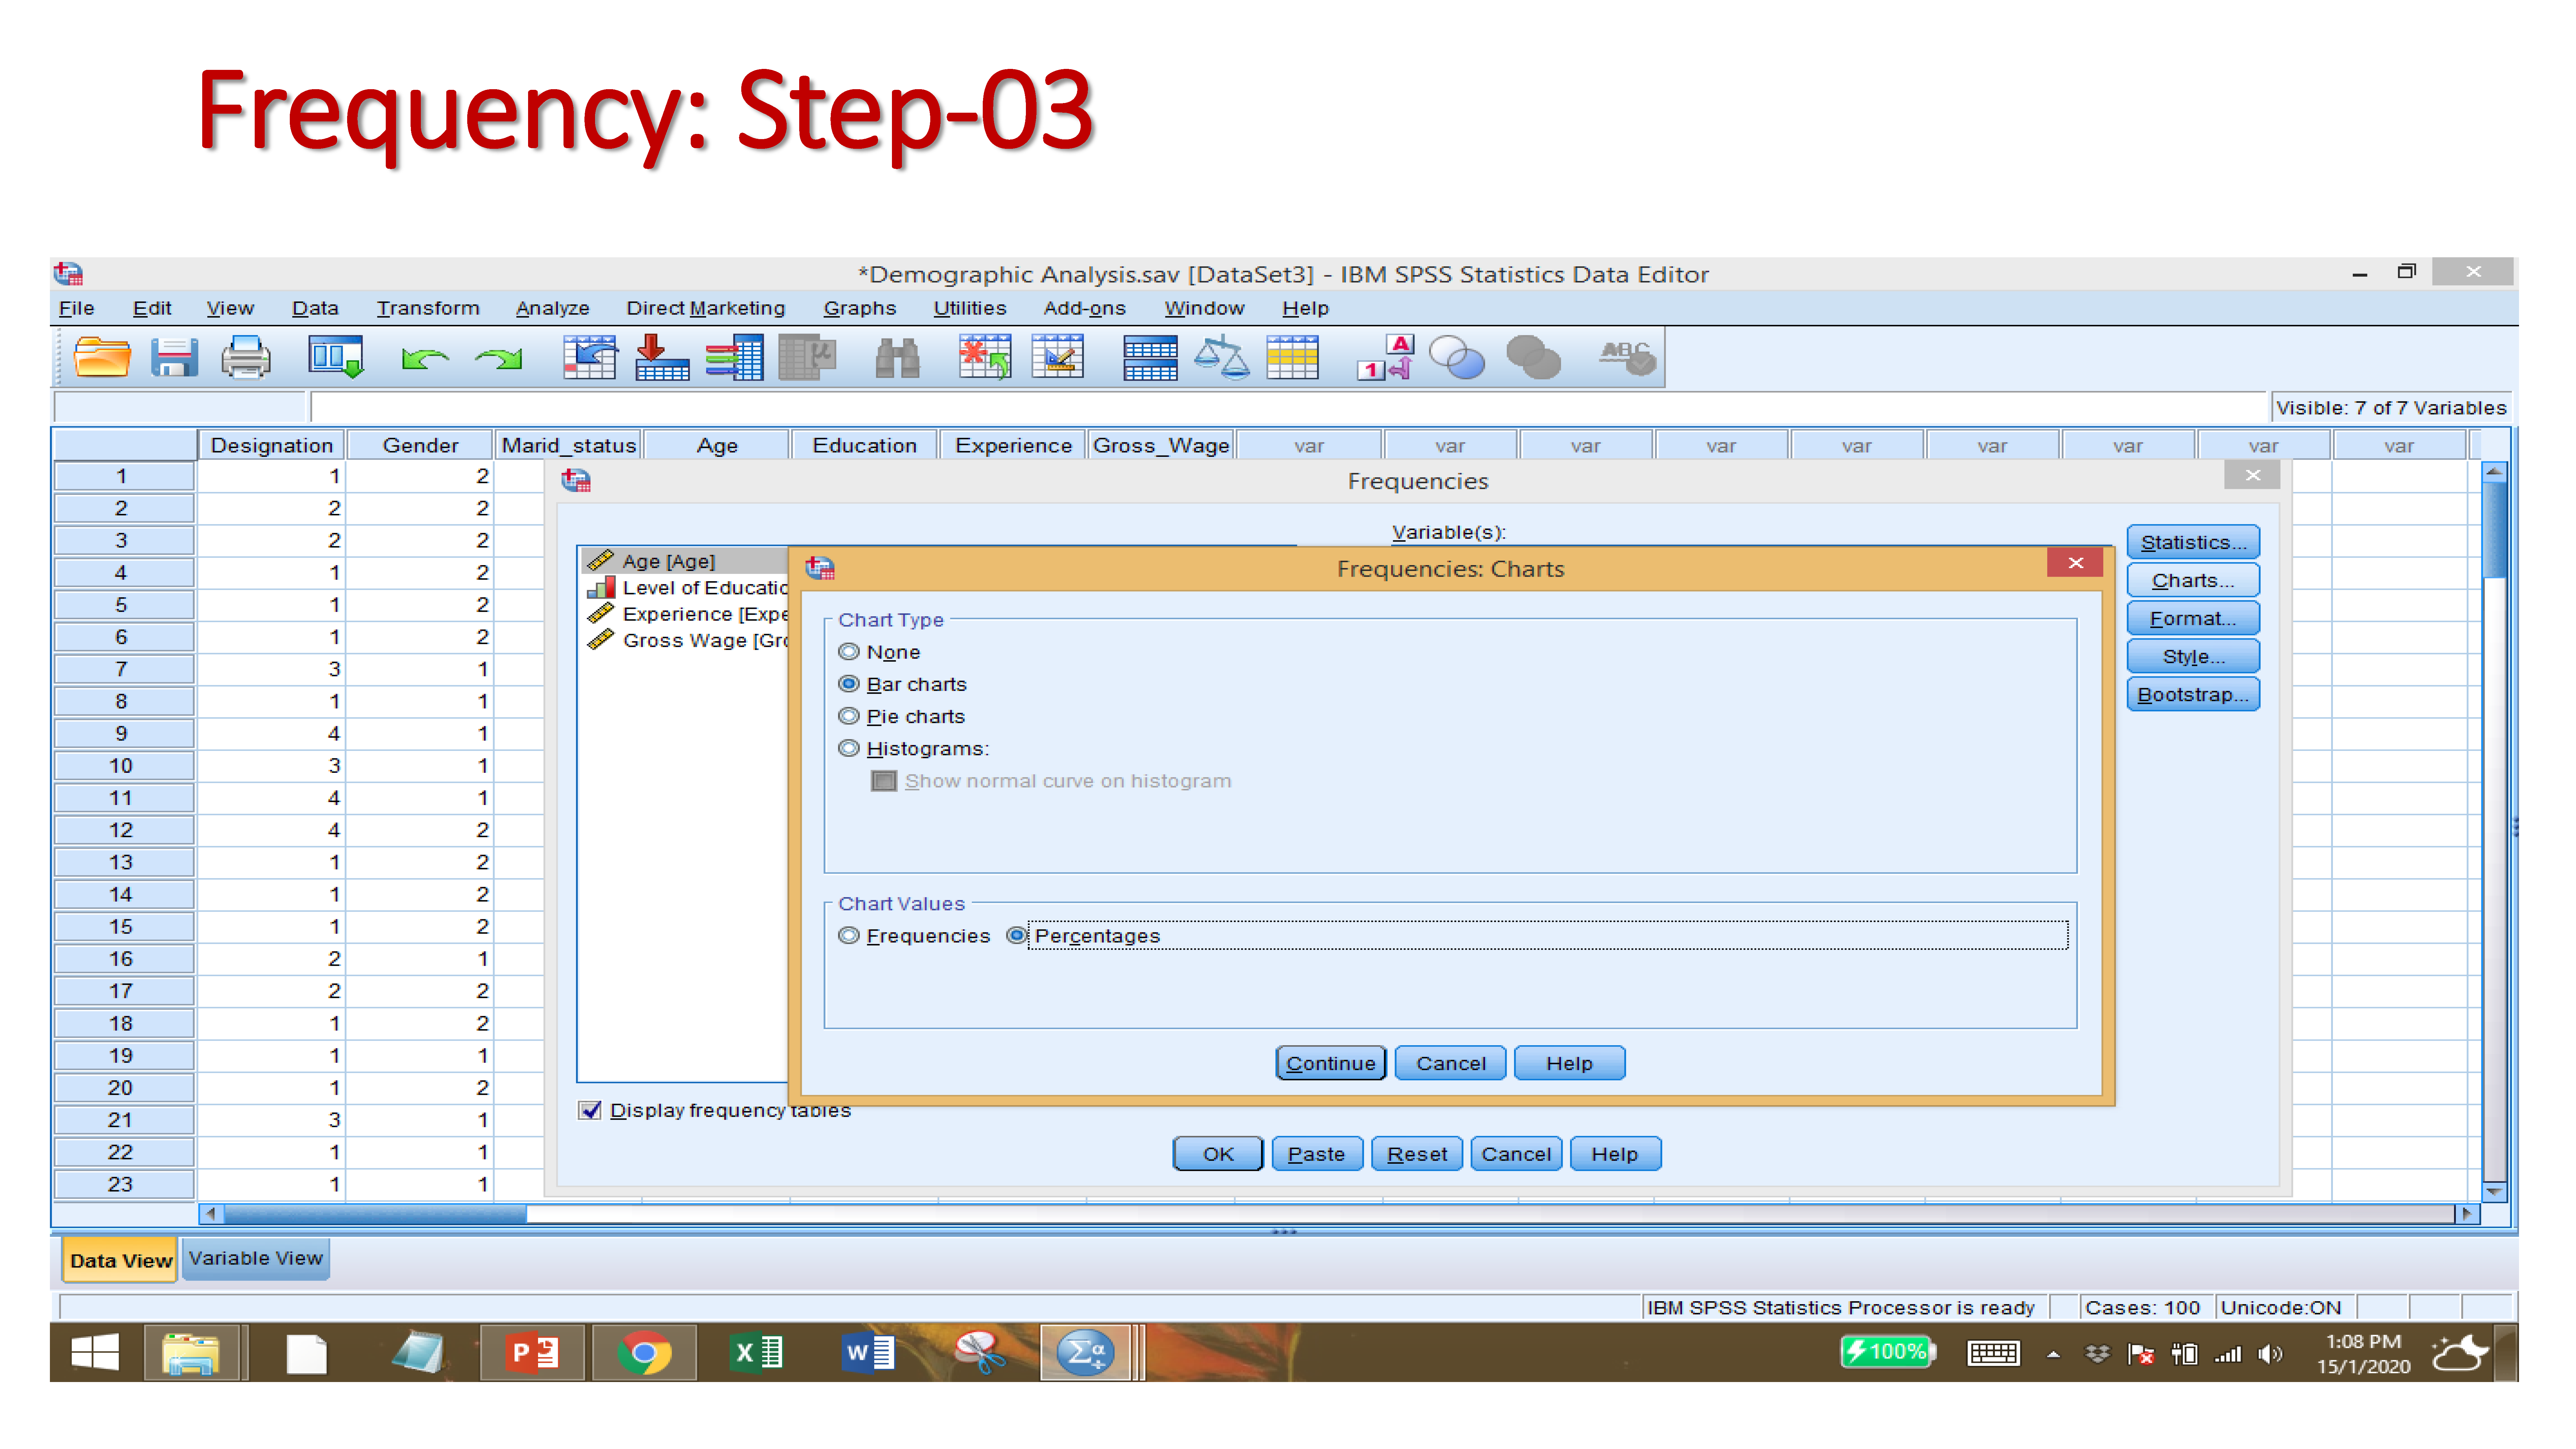
\includegraphics{images/slides/img_Page_028.png}

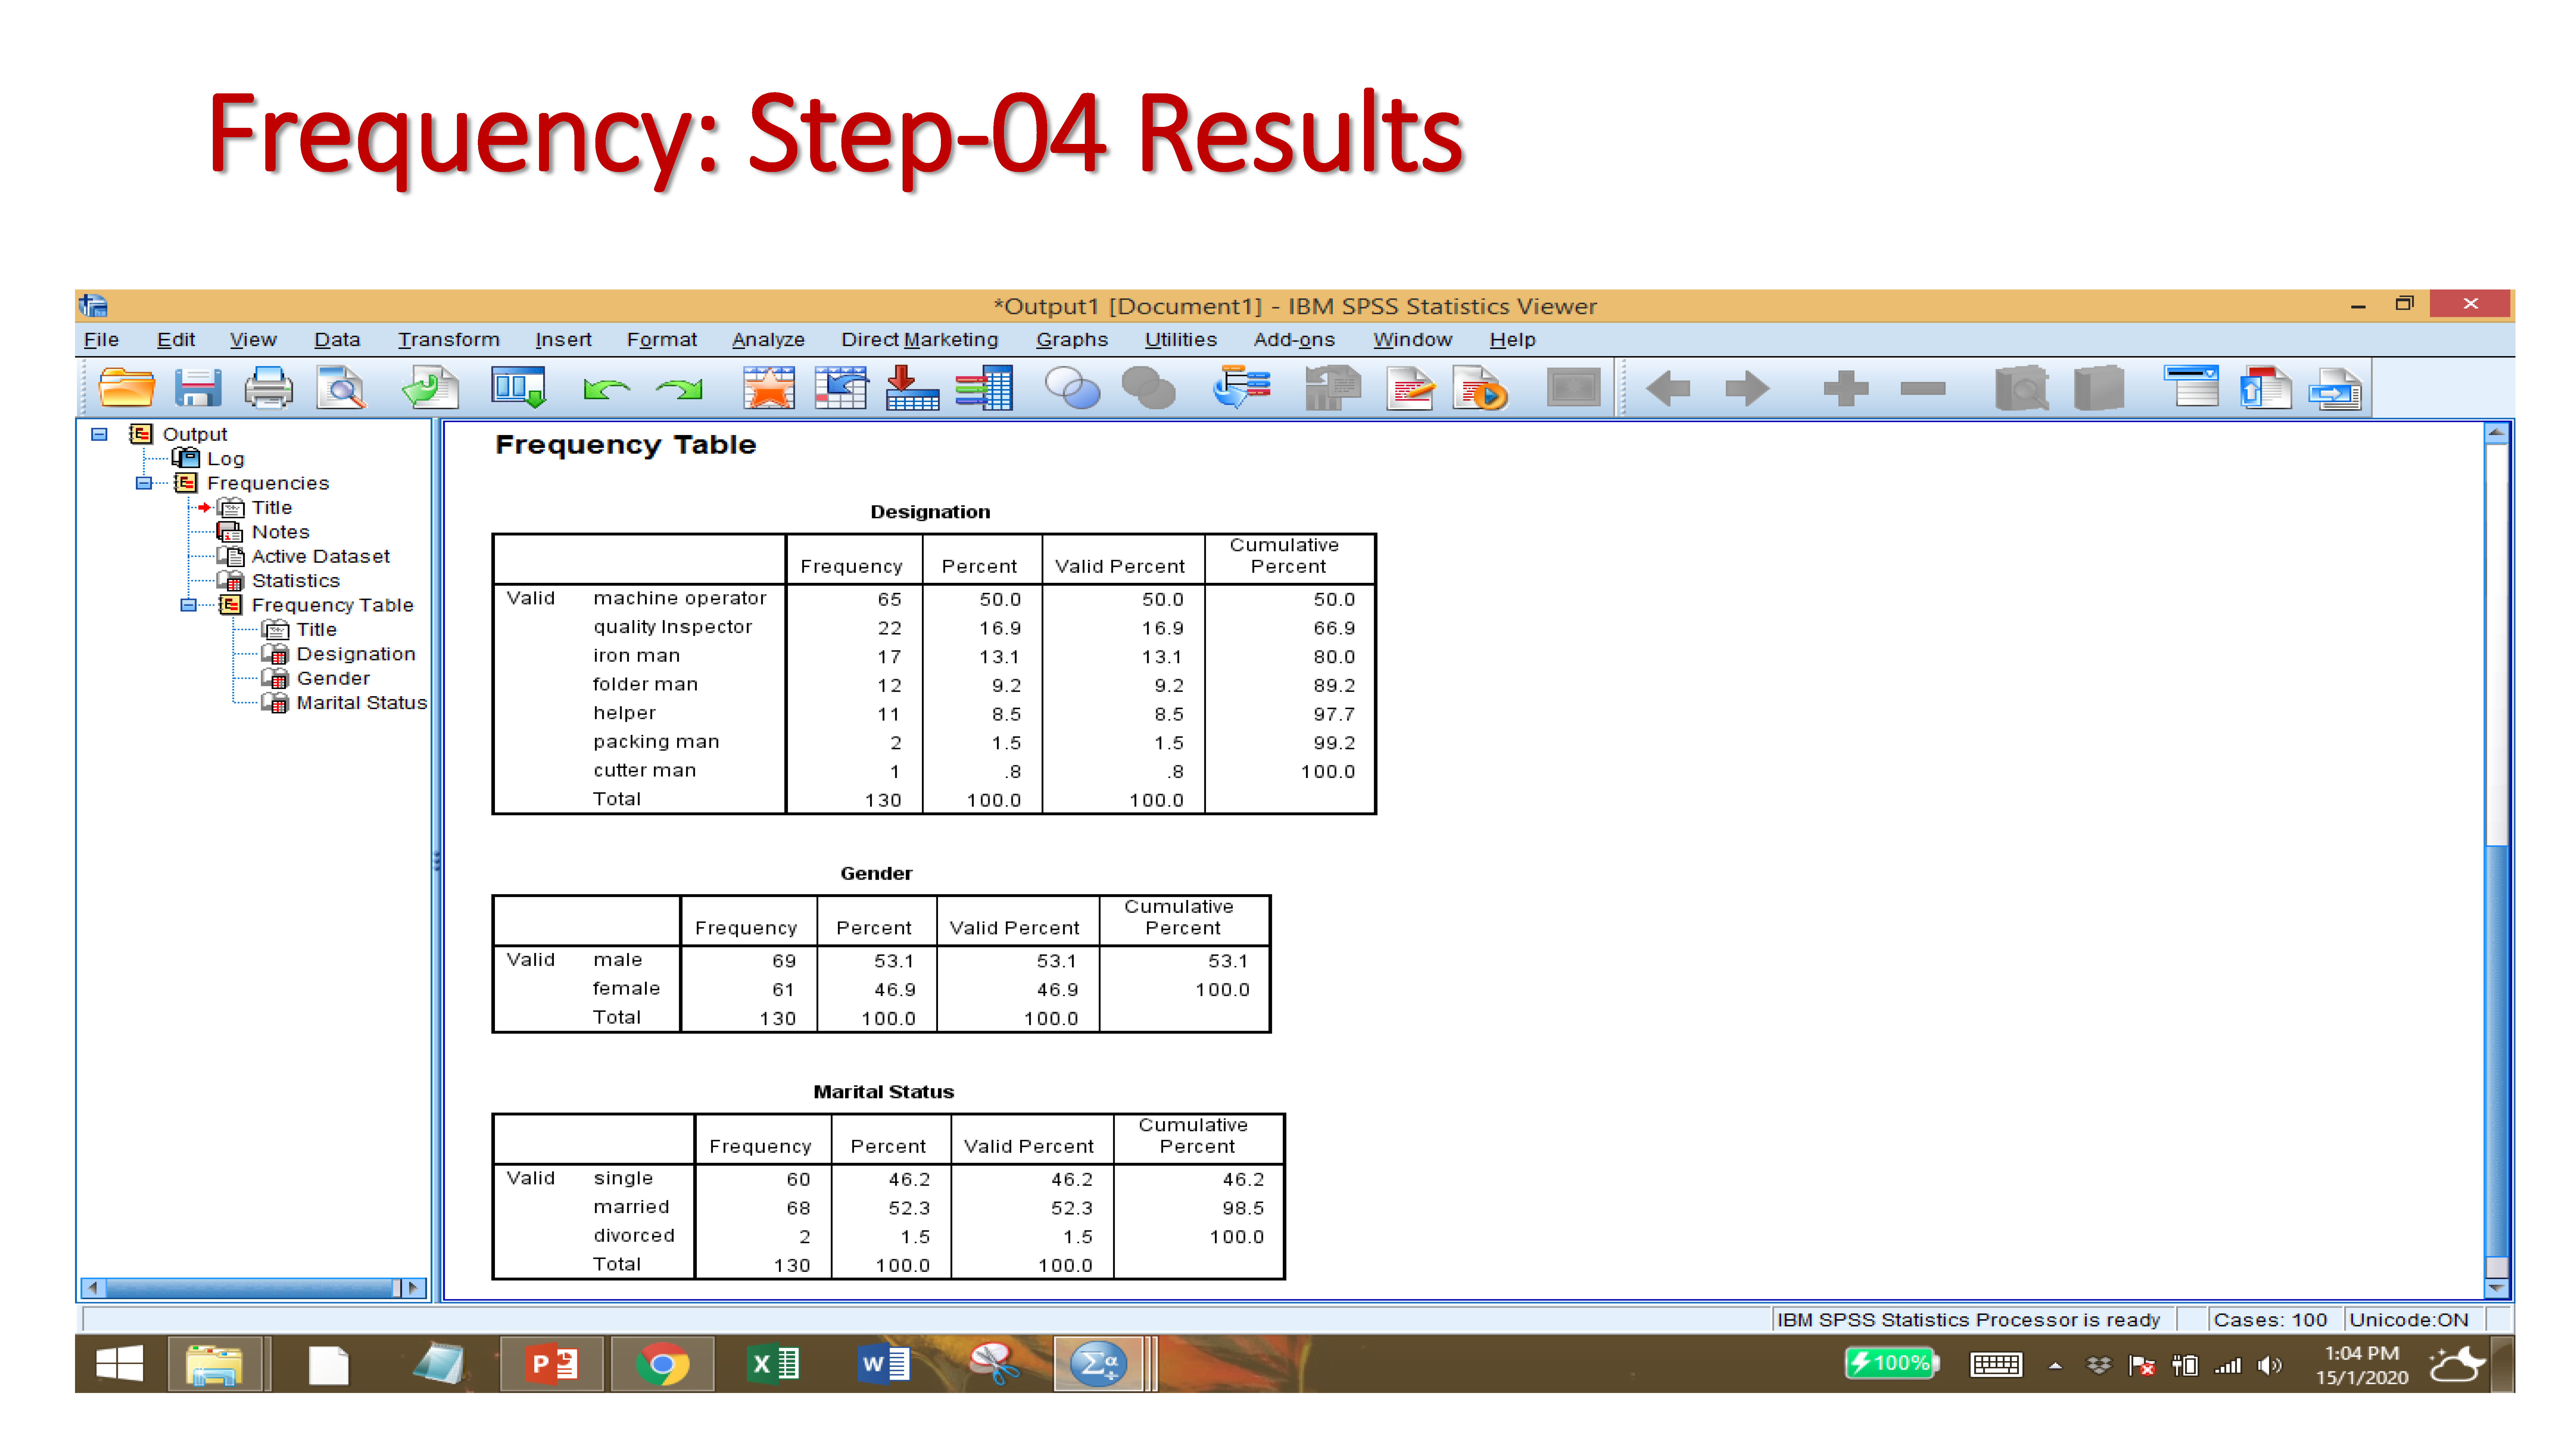
\includegraphics{images/slides/img_Page_029.png}

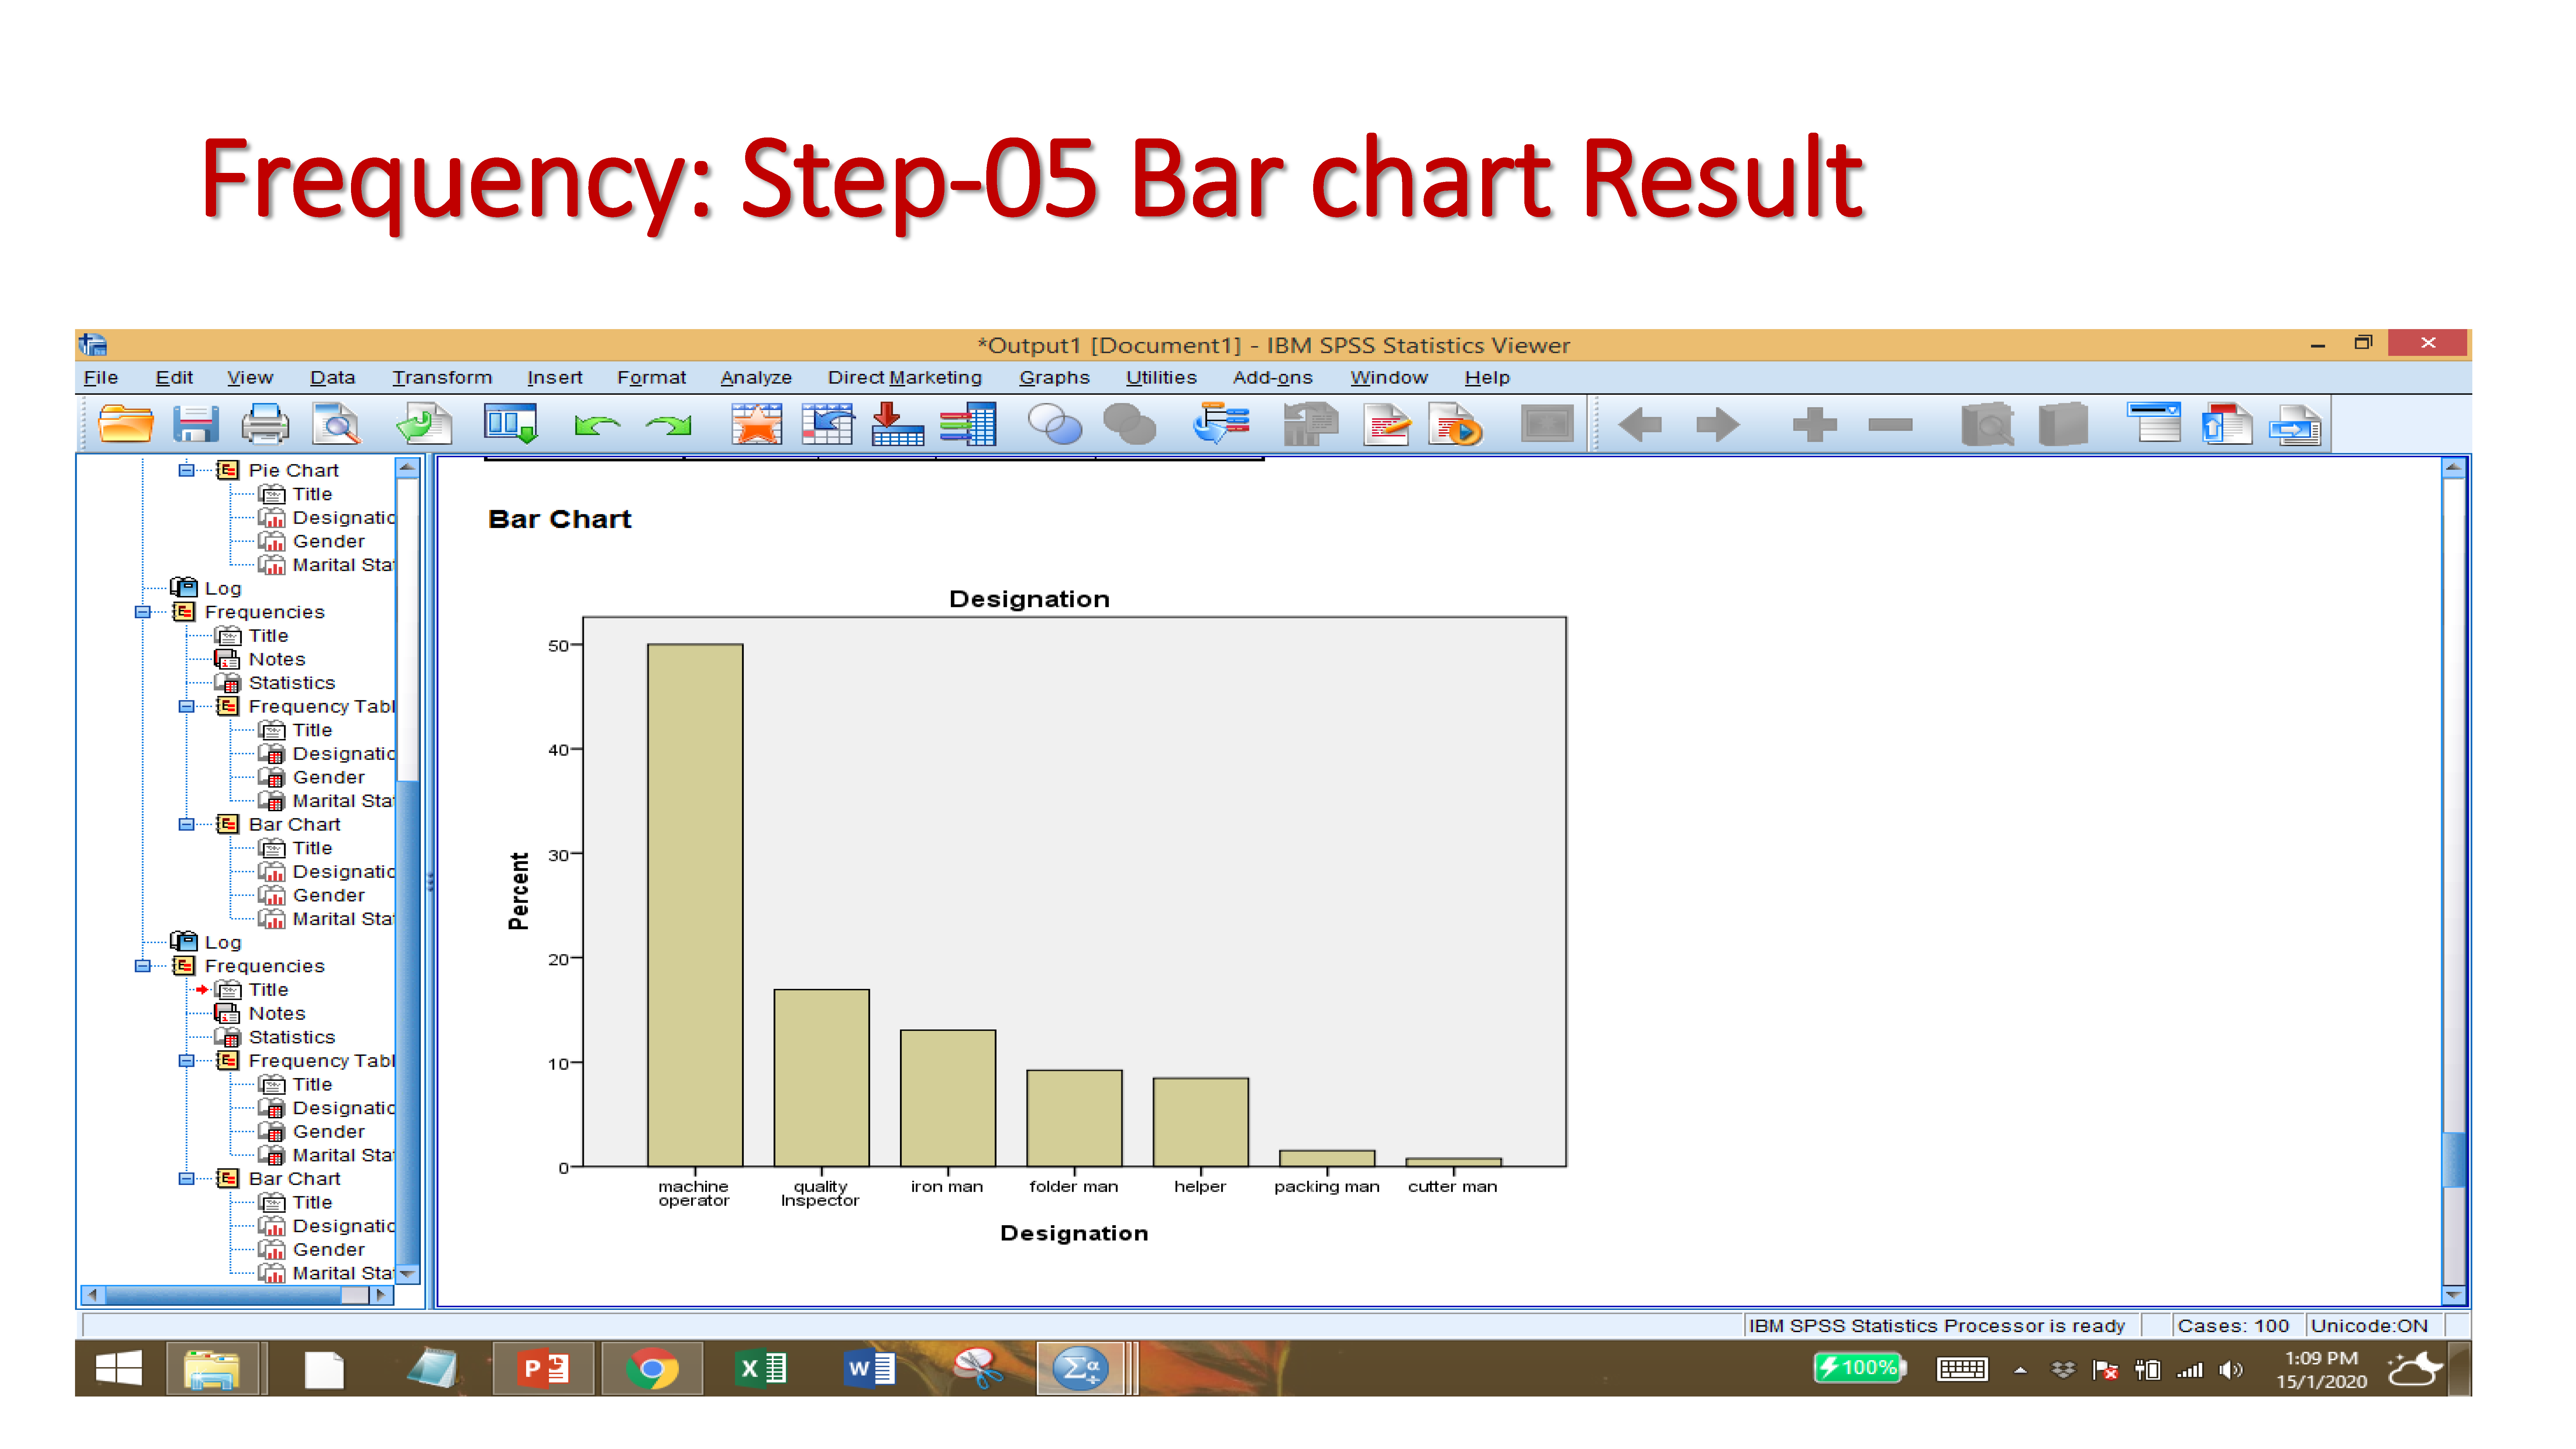
\includegraphics{images/slides/img_Page_030.png}

\section{Numerical Data}\label{numerical-data}

After Importing your dataset, and providing names to variables, click
on:\\

{ANALYZE → DESCRIPTIVE STATISTICS → DESCRIPTIVES}

Choose any variables to be analyzed and place them in box on right
Options include:

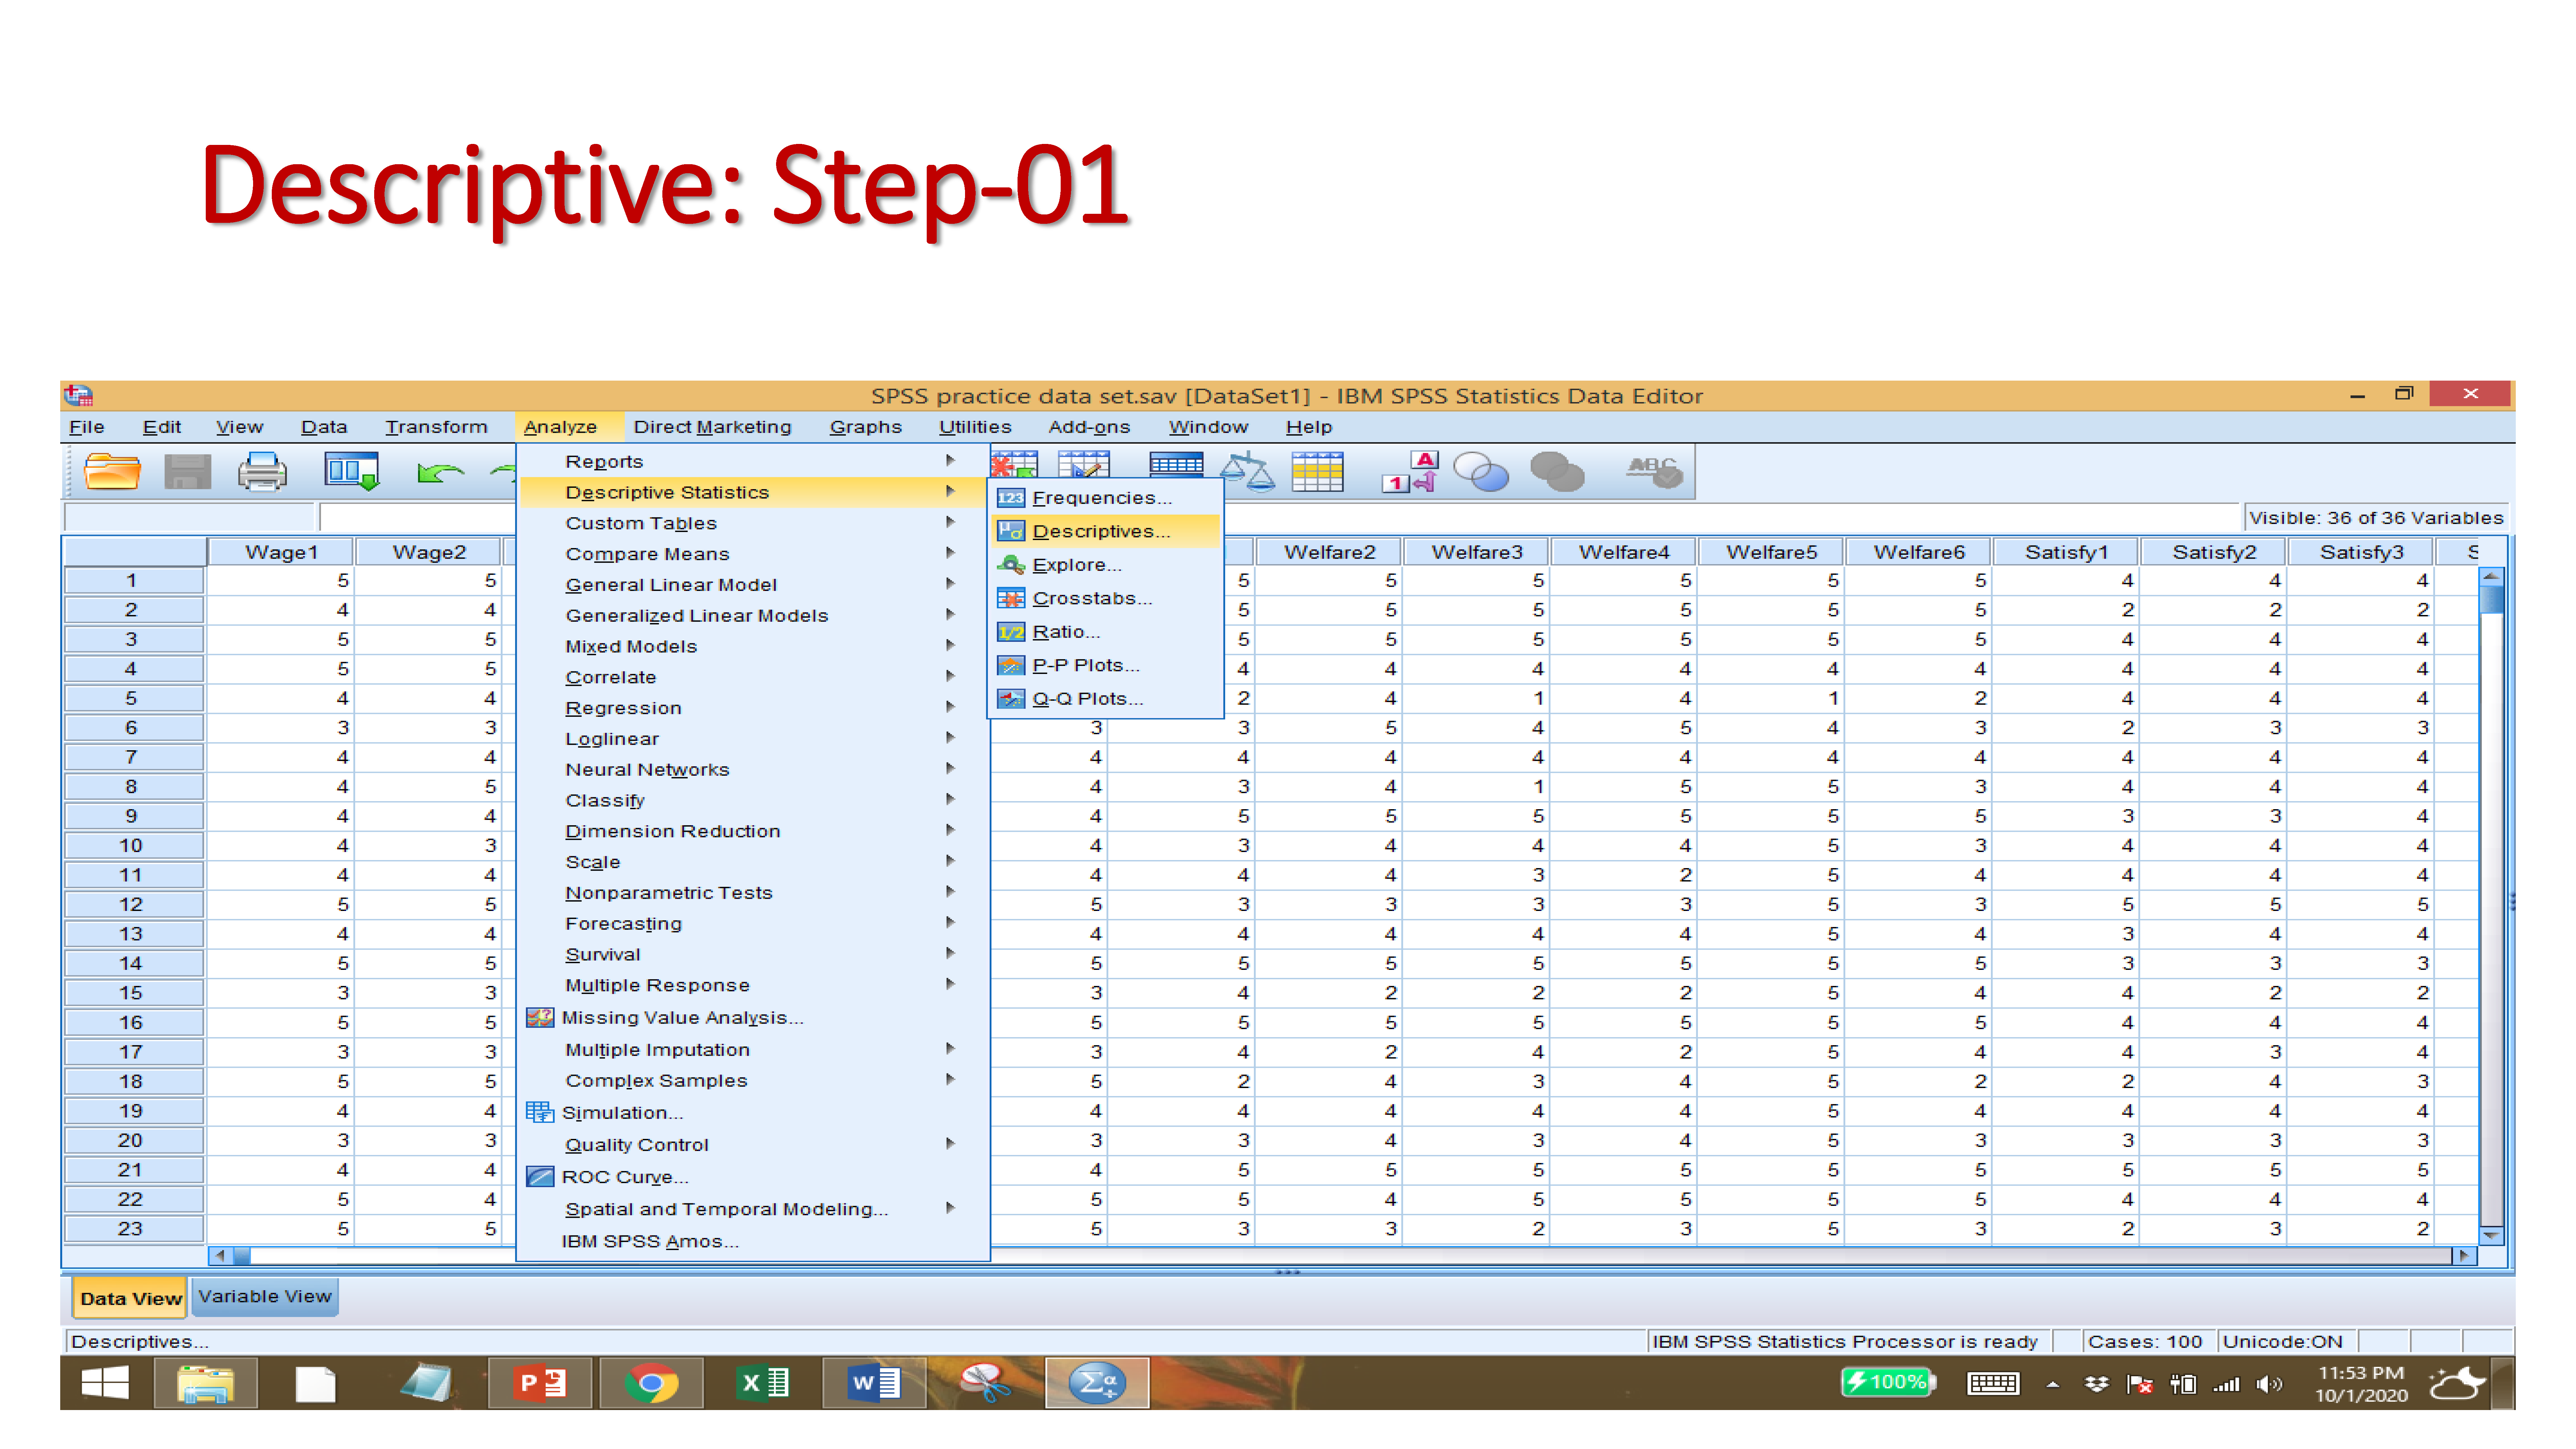
\includegraphics{images/slides/img_Page_032.png}

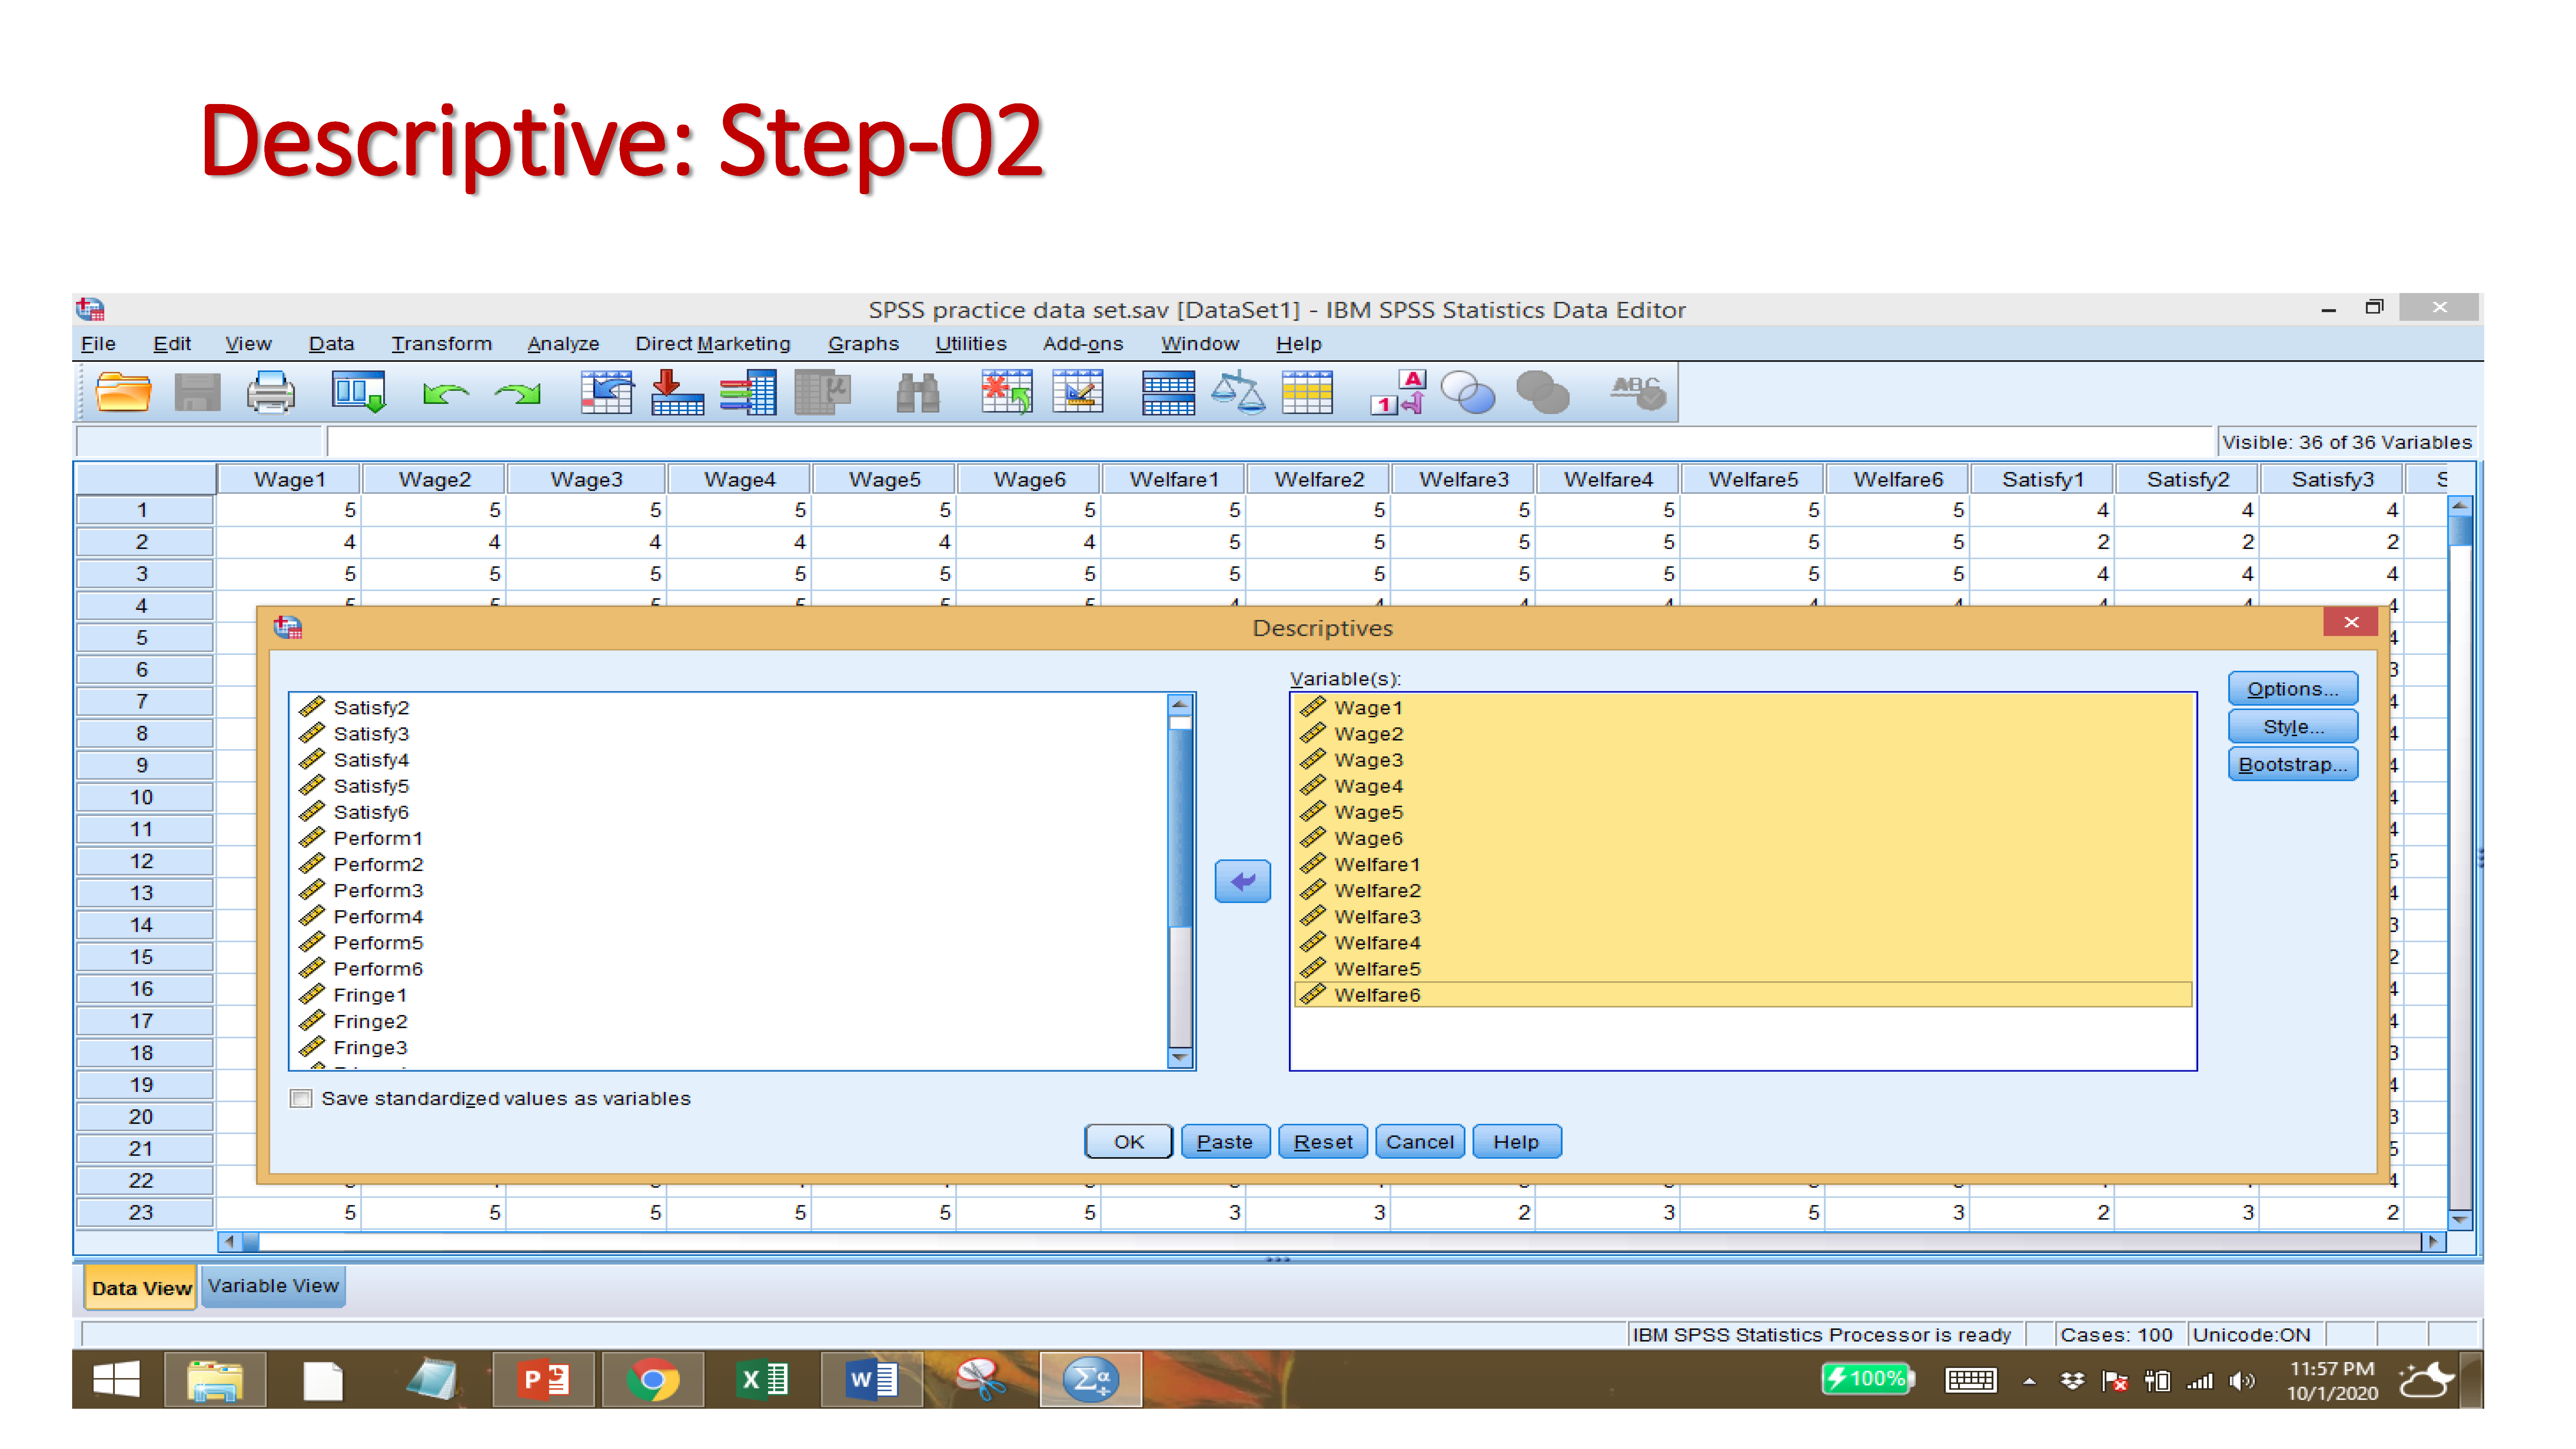
\includegraphics{images/slides/img_Page_033.png}

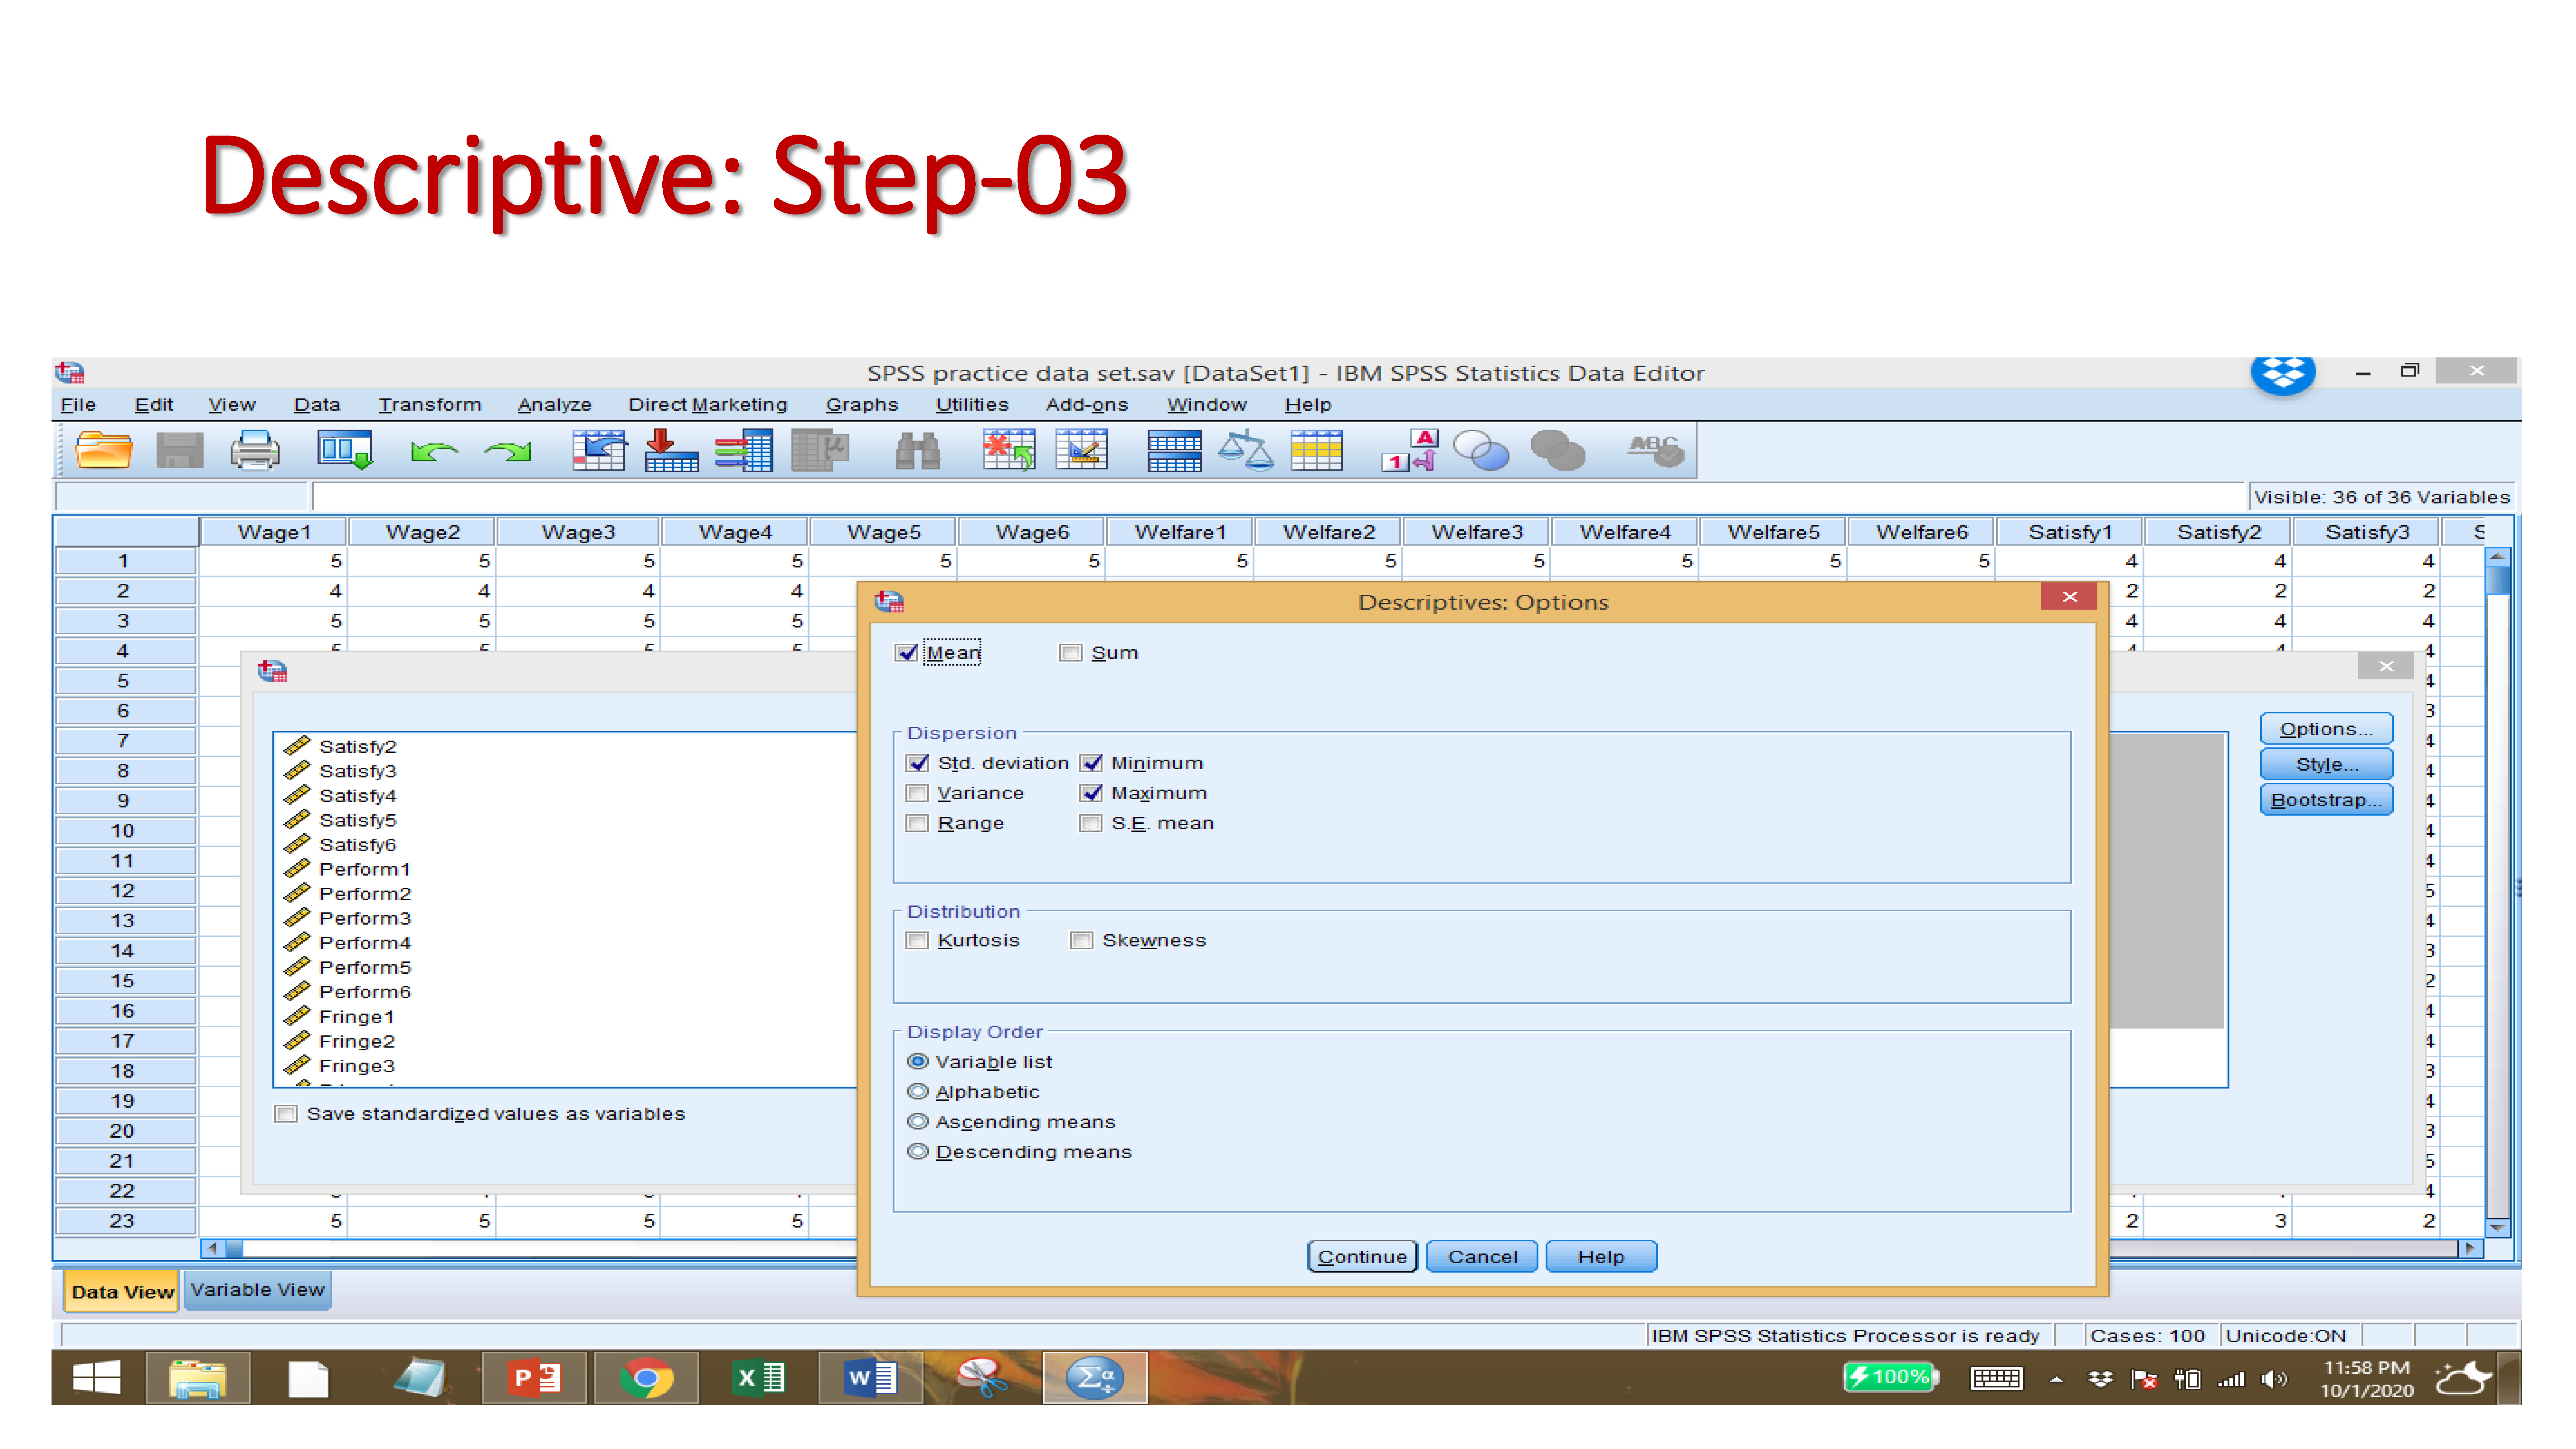
\includegraphics{images/slides/img_Page_034.png}

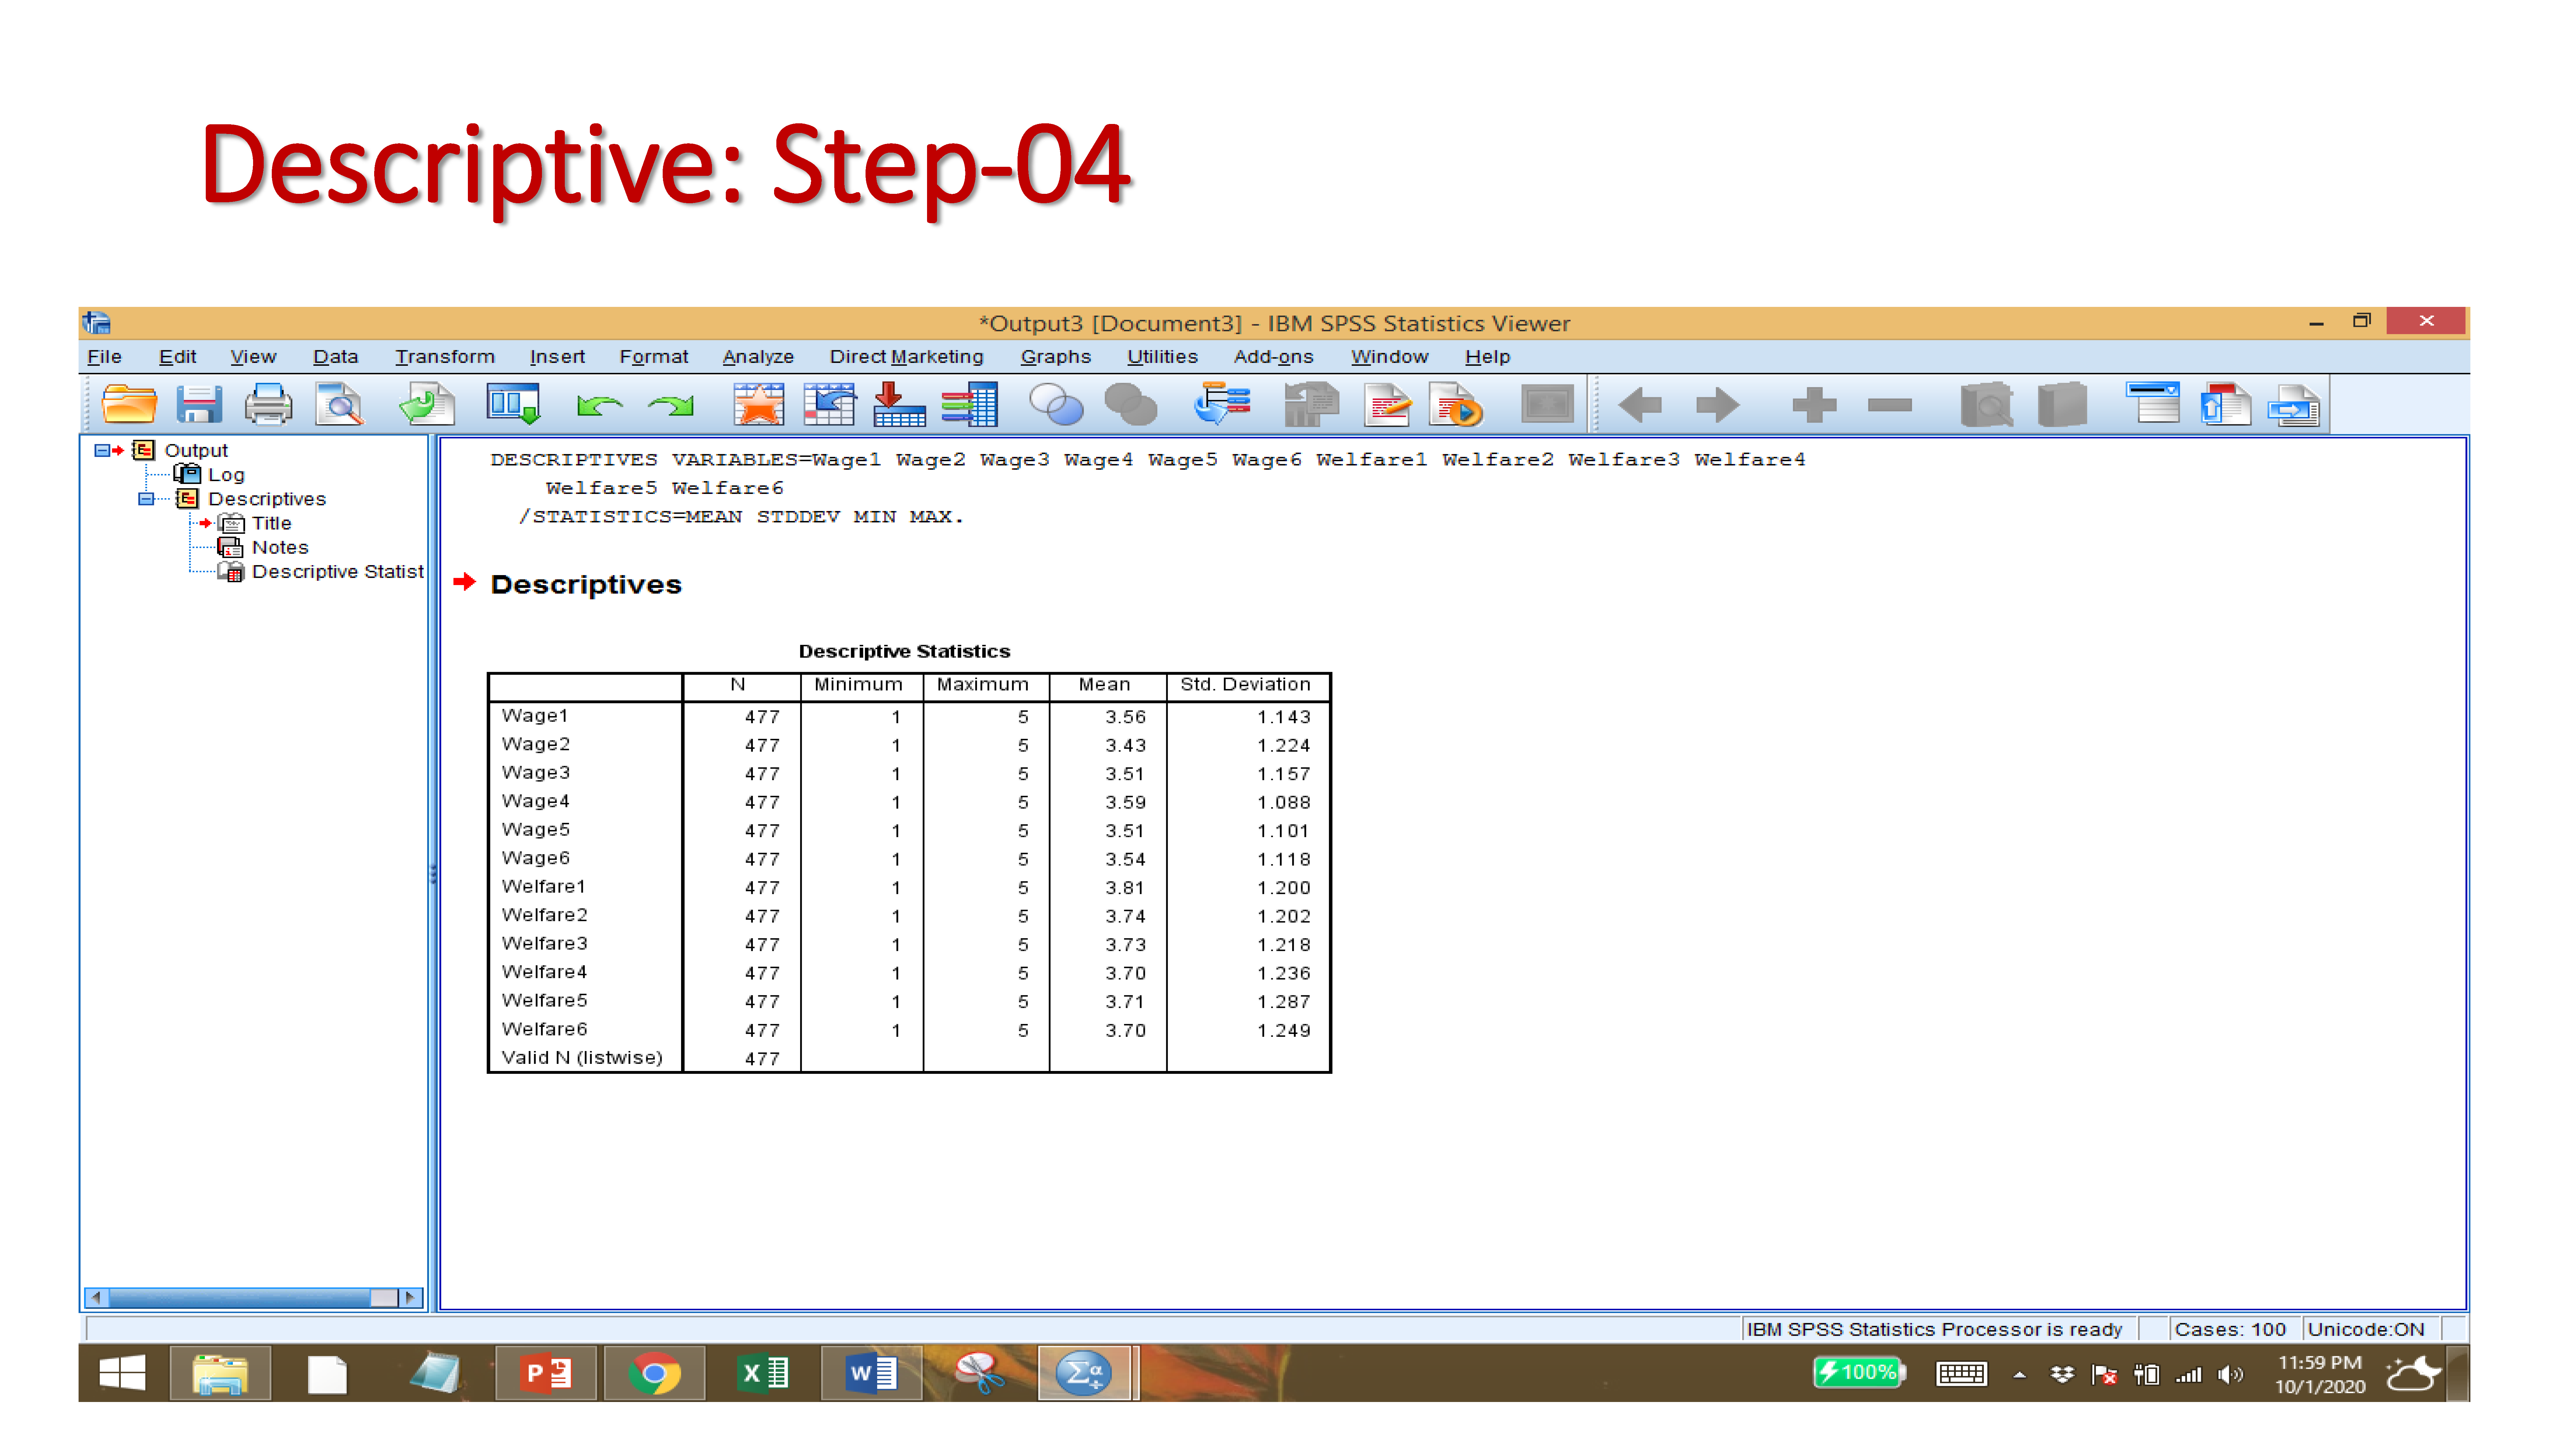
\includegraphics{images/slides/img_Page_035.png}

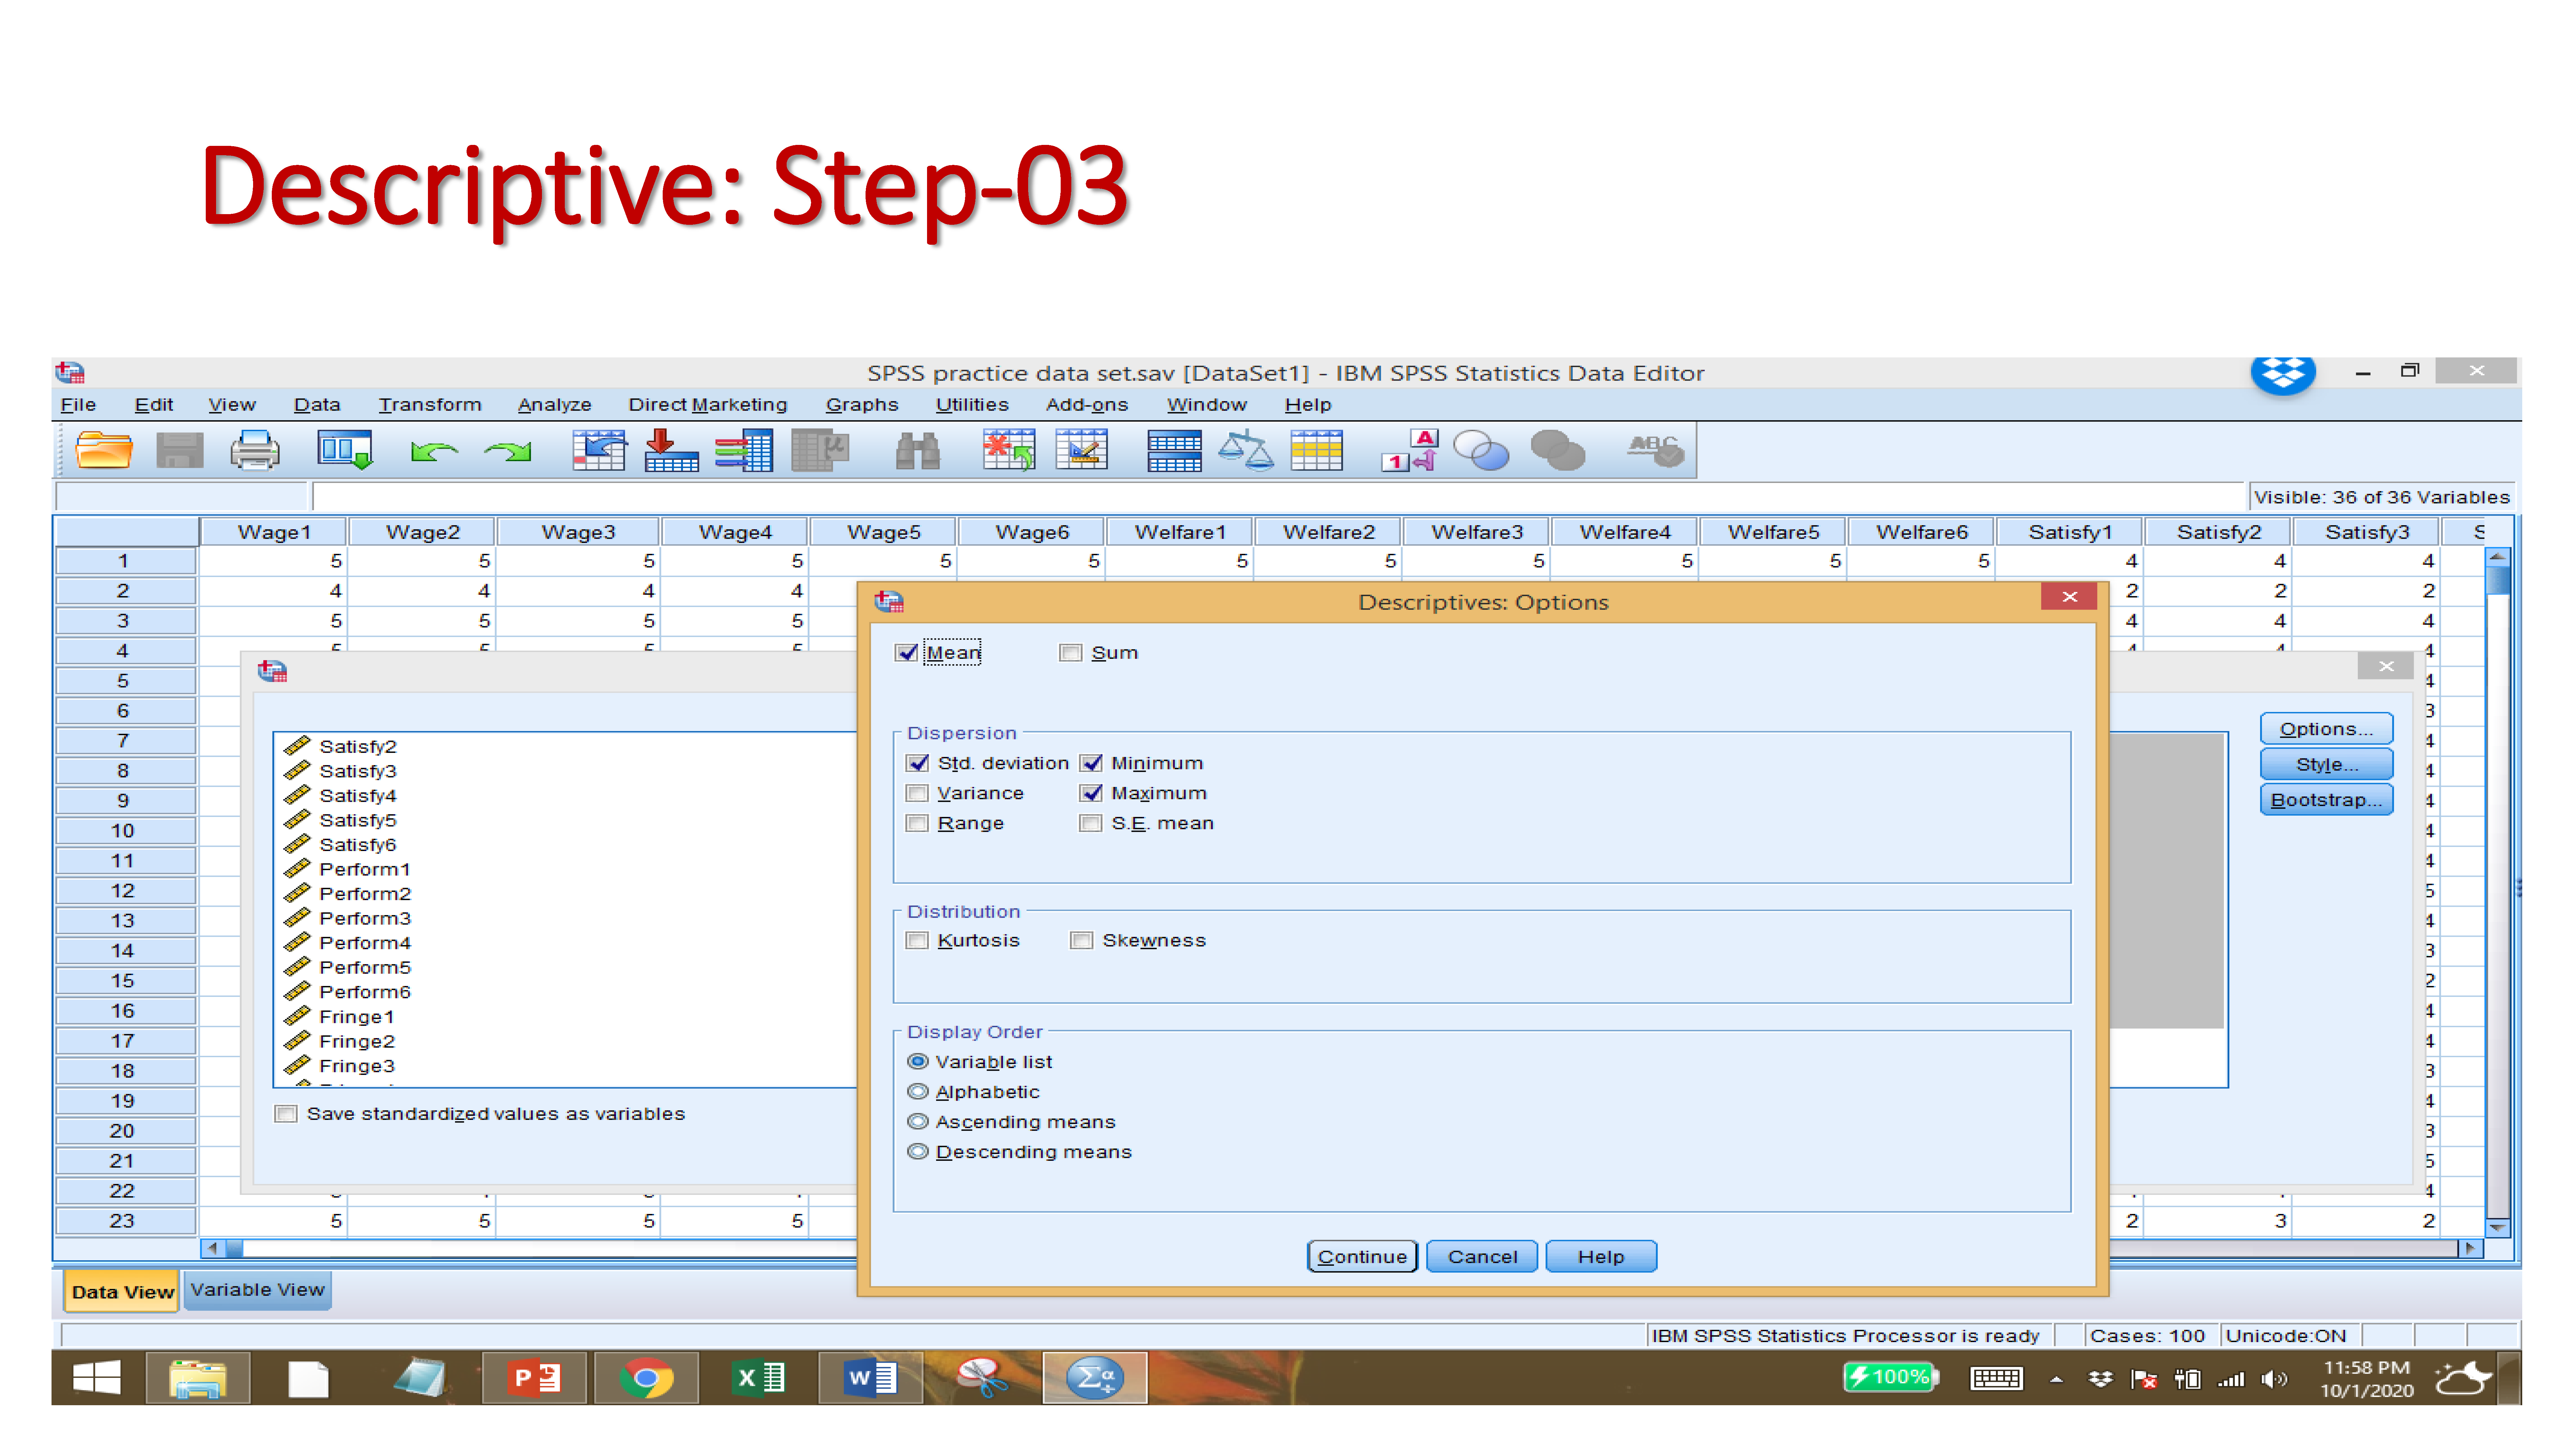
\includegraphics{images/slides/img_Page_036.png}

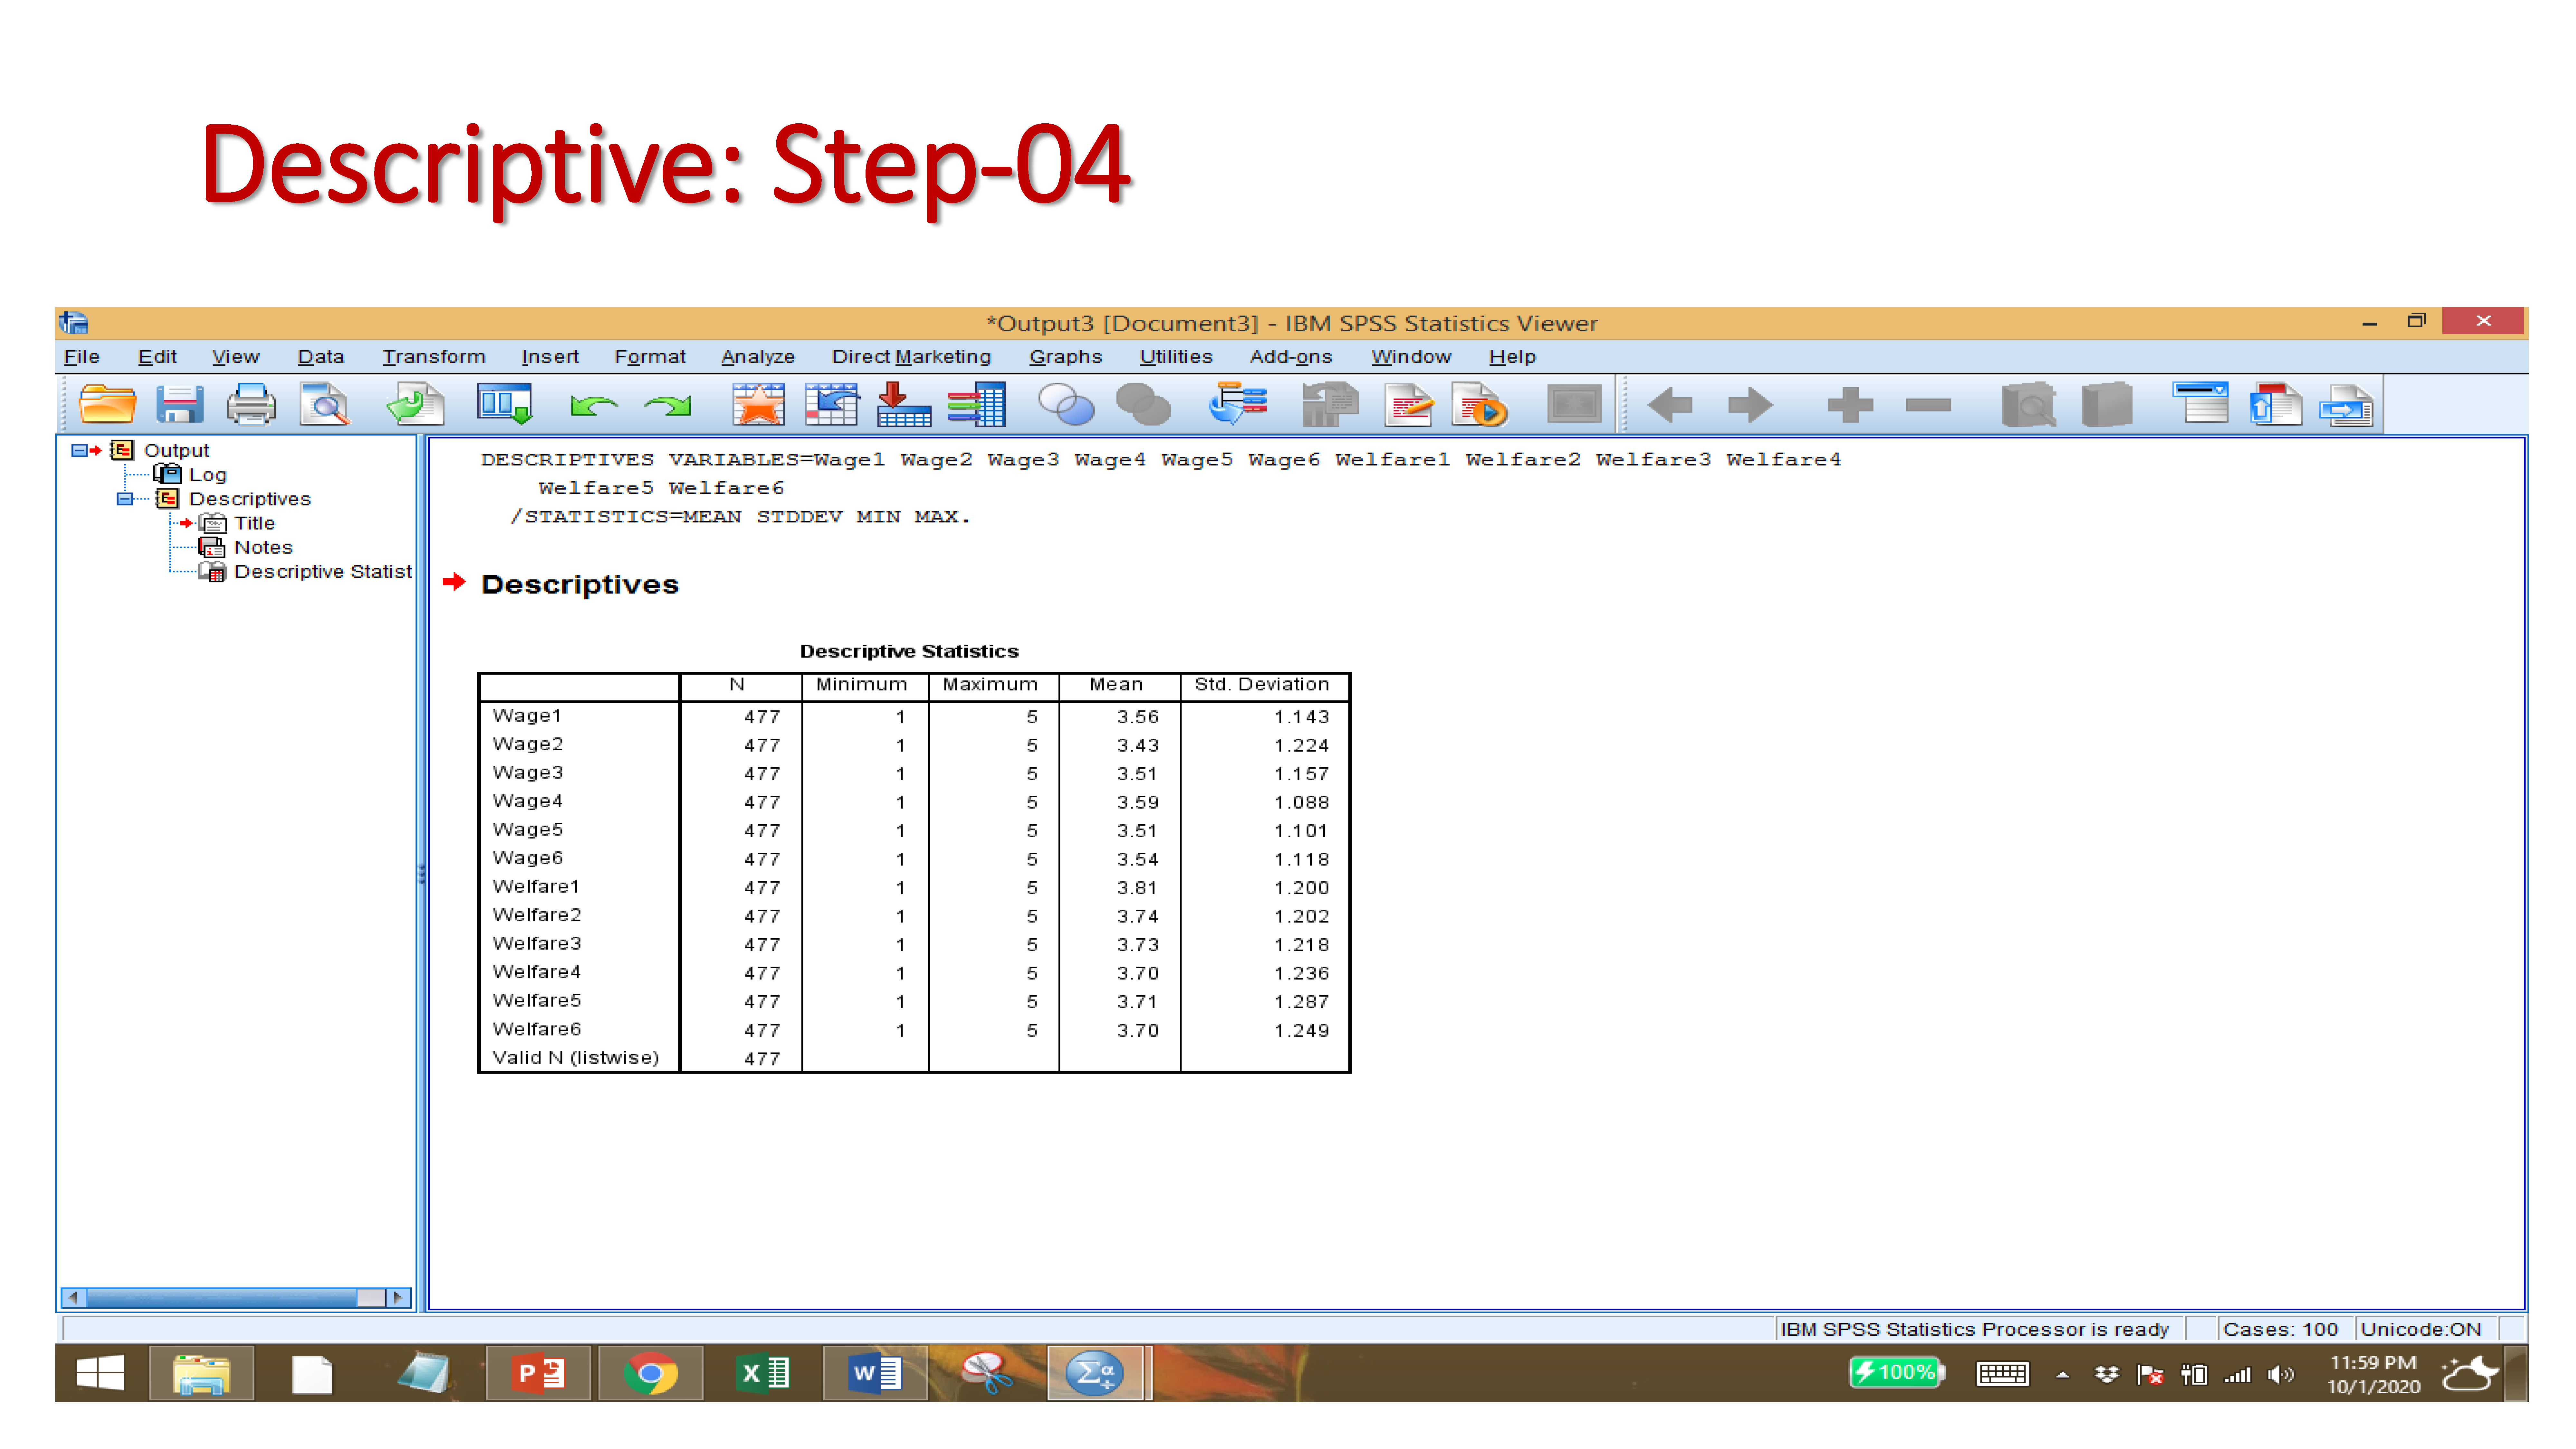
\includegraphics{images/slides/img_Page_037.png}

\bookmarksetup{startatroot}

\chapter{Test of Data Normality}\label{test-of-data-normality}

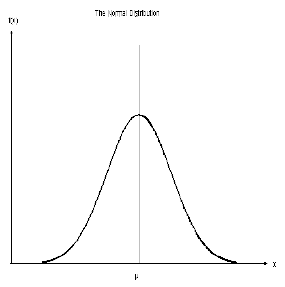
\includegraphics{images/normal.png}

``Normal'' data are data that are drawn (come from) a population that
has a normal distribution. This distribution is unarguably the most
important and the most frequently used distribution in both the theory
and application of statistics. There are two types of data normality;\\

\begin{enumerate}
\def\labelenumi{\arabic{enumi}.}
\tightlist
\item
  Univariate data normality (Skewness \& Kurtosis)\\
\item
  Multivariate data normality (Mardia Test)\\
\end{enumerate}

\bookmarksetup{startatroot}

\chapter{Test of outliers}\label{test-of-outliers}

{In statistics, an outlier is a data point that differs significantly
from other observations. An outlier may be due to variability in the
measurement or it may indicate experimental error; the outlers are
sometimes excluded from the data set. An outlier can cause serious
problems in statistical analyses.}\\

{There are two types of outliers;}\\
{1. Univariate outliers (Z-Score)\\
2. Multivariate outliers (Mahalanobis Distance)}\\

{A univariate outlier is a data point that consists of an extreme value
on one variable. A multivariate outlier is a combination of unusual
scores on at least two variables. Both types of outliers can influence
the outcome of statistical analyses.}\\

\section{Test of Univariate outliers}\label{test-of-univariate-outliers}

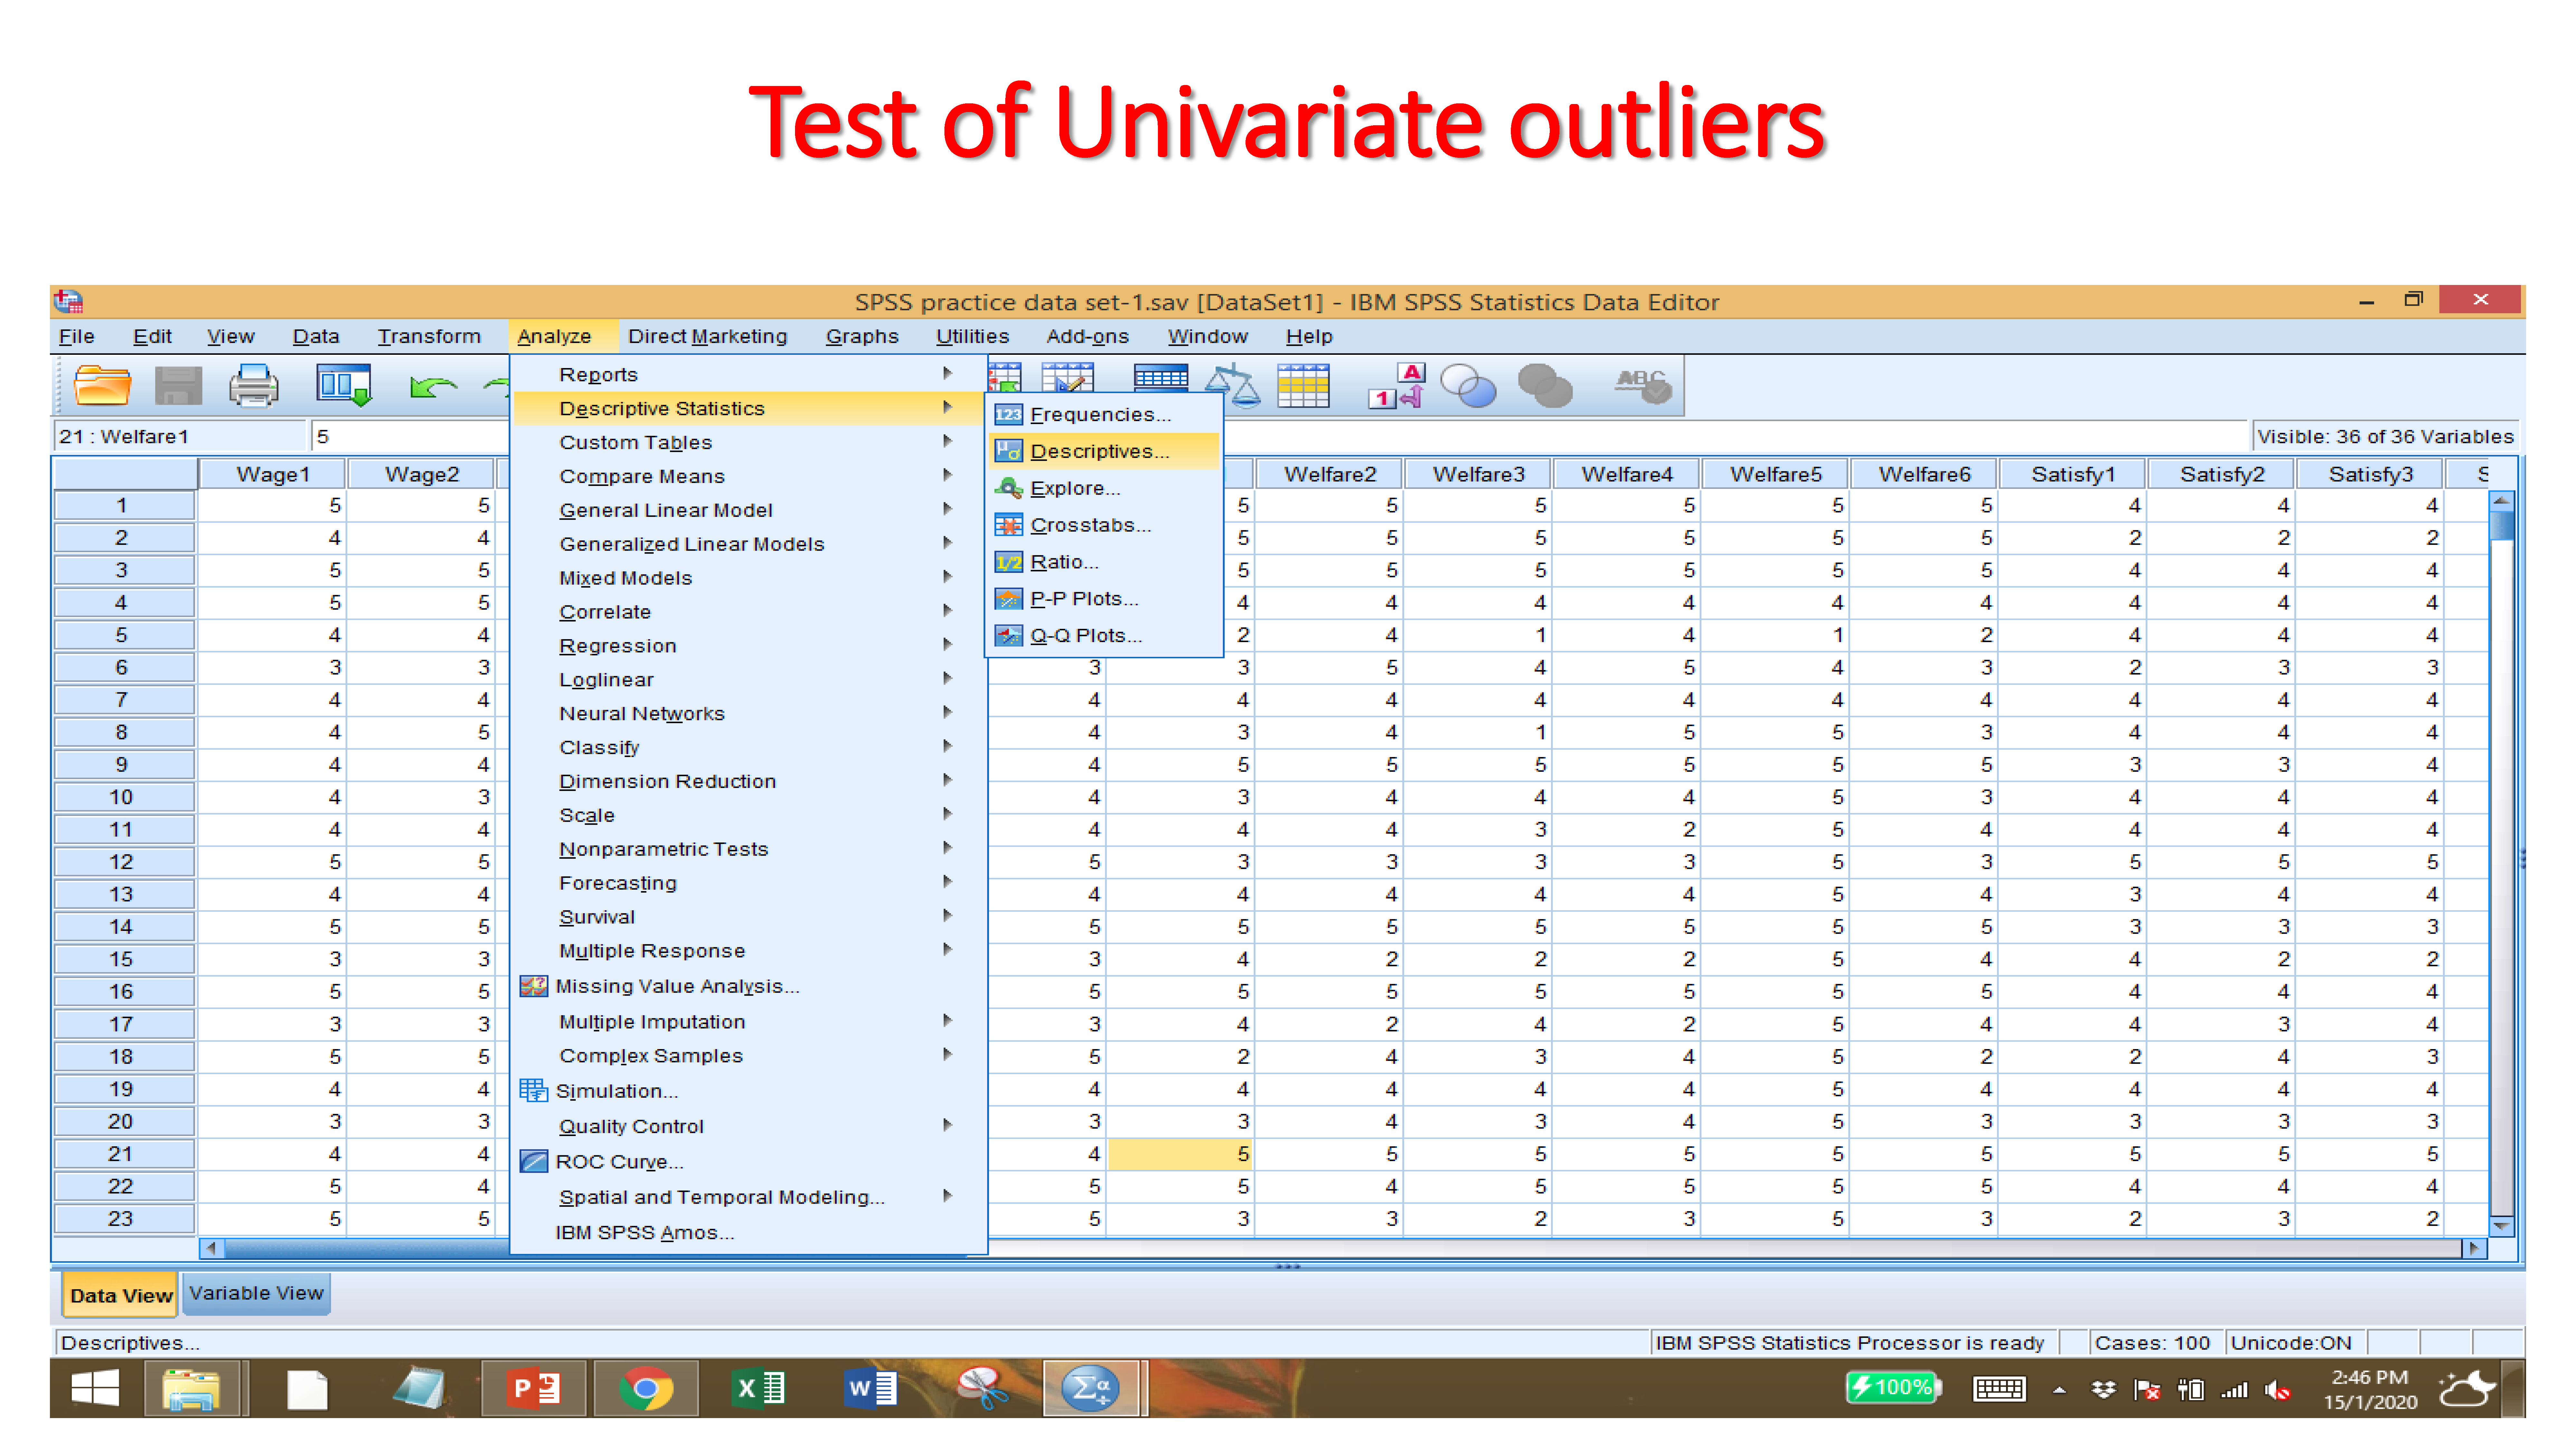
\includegraphics{images/slides/img_Page_040.png}

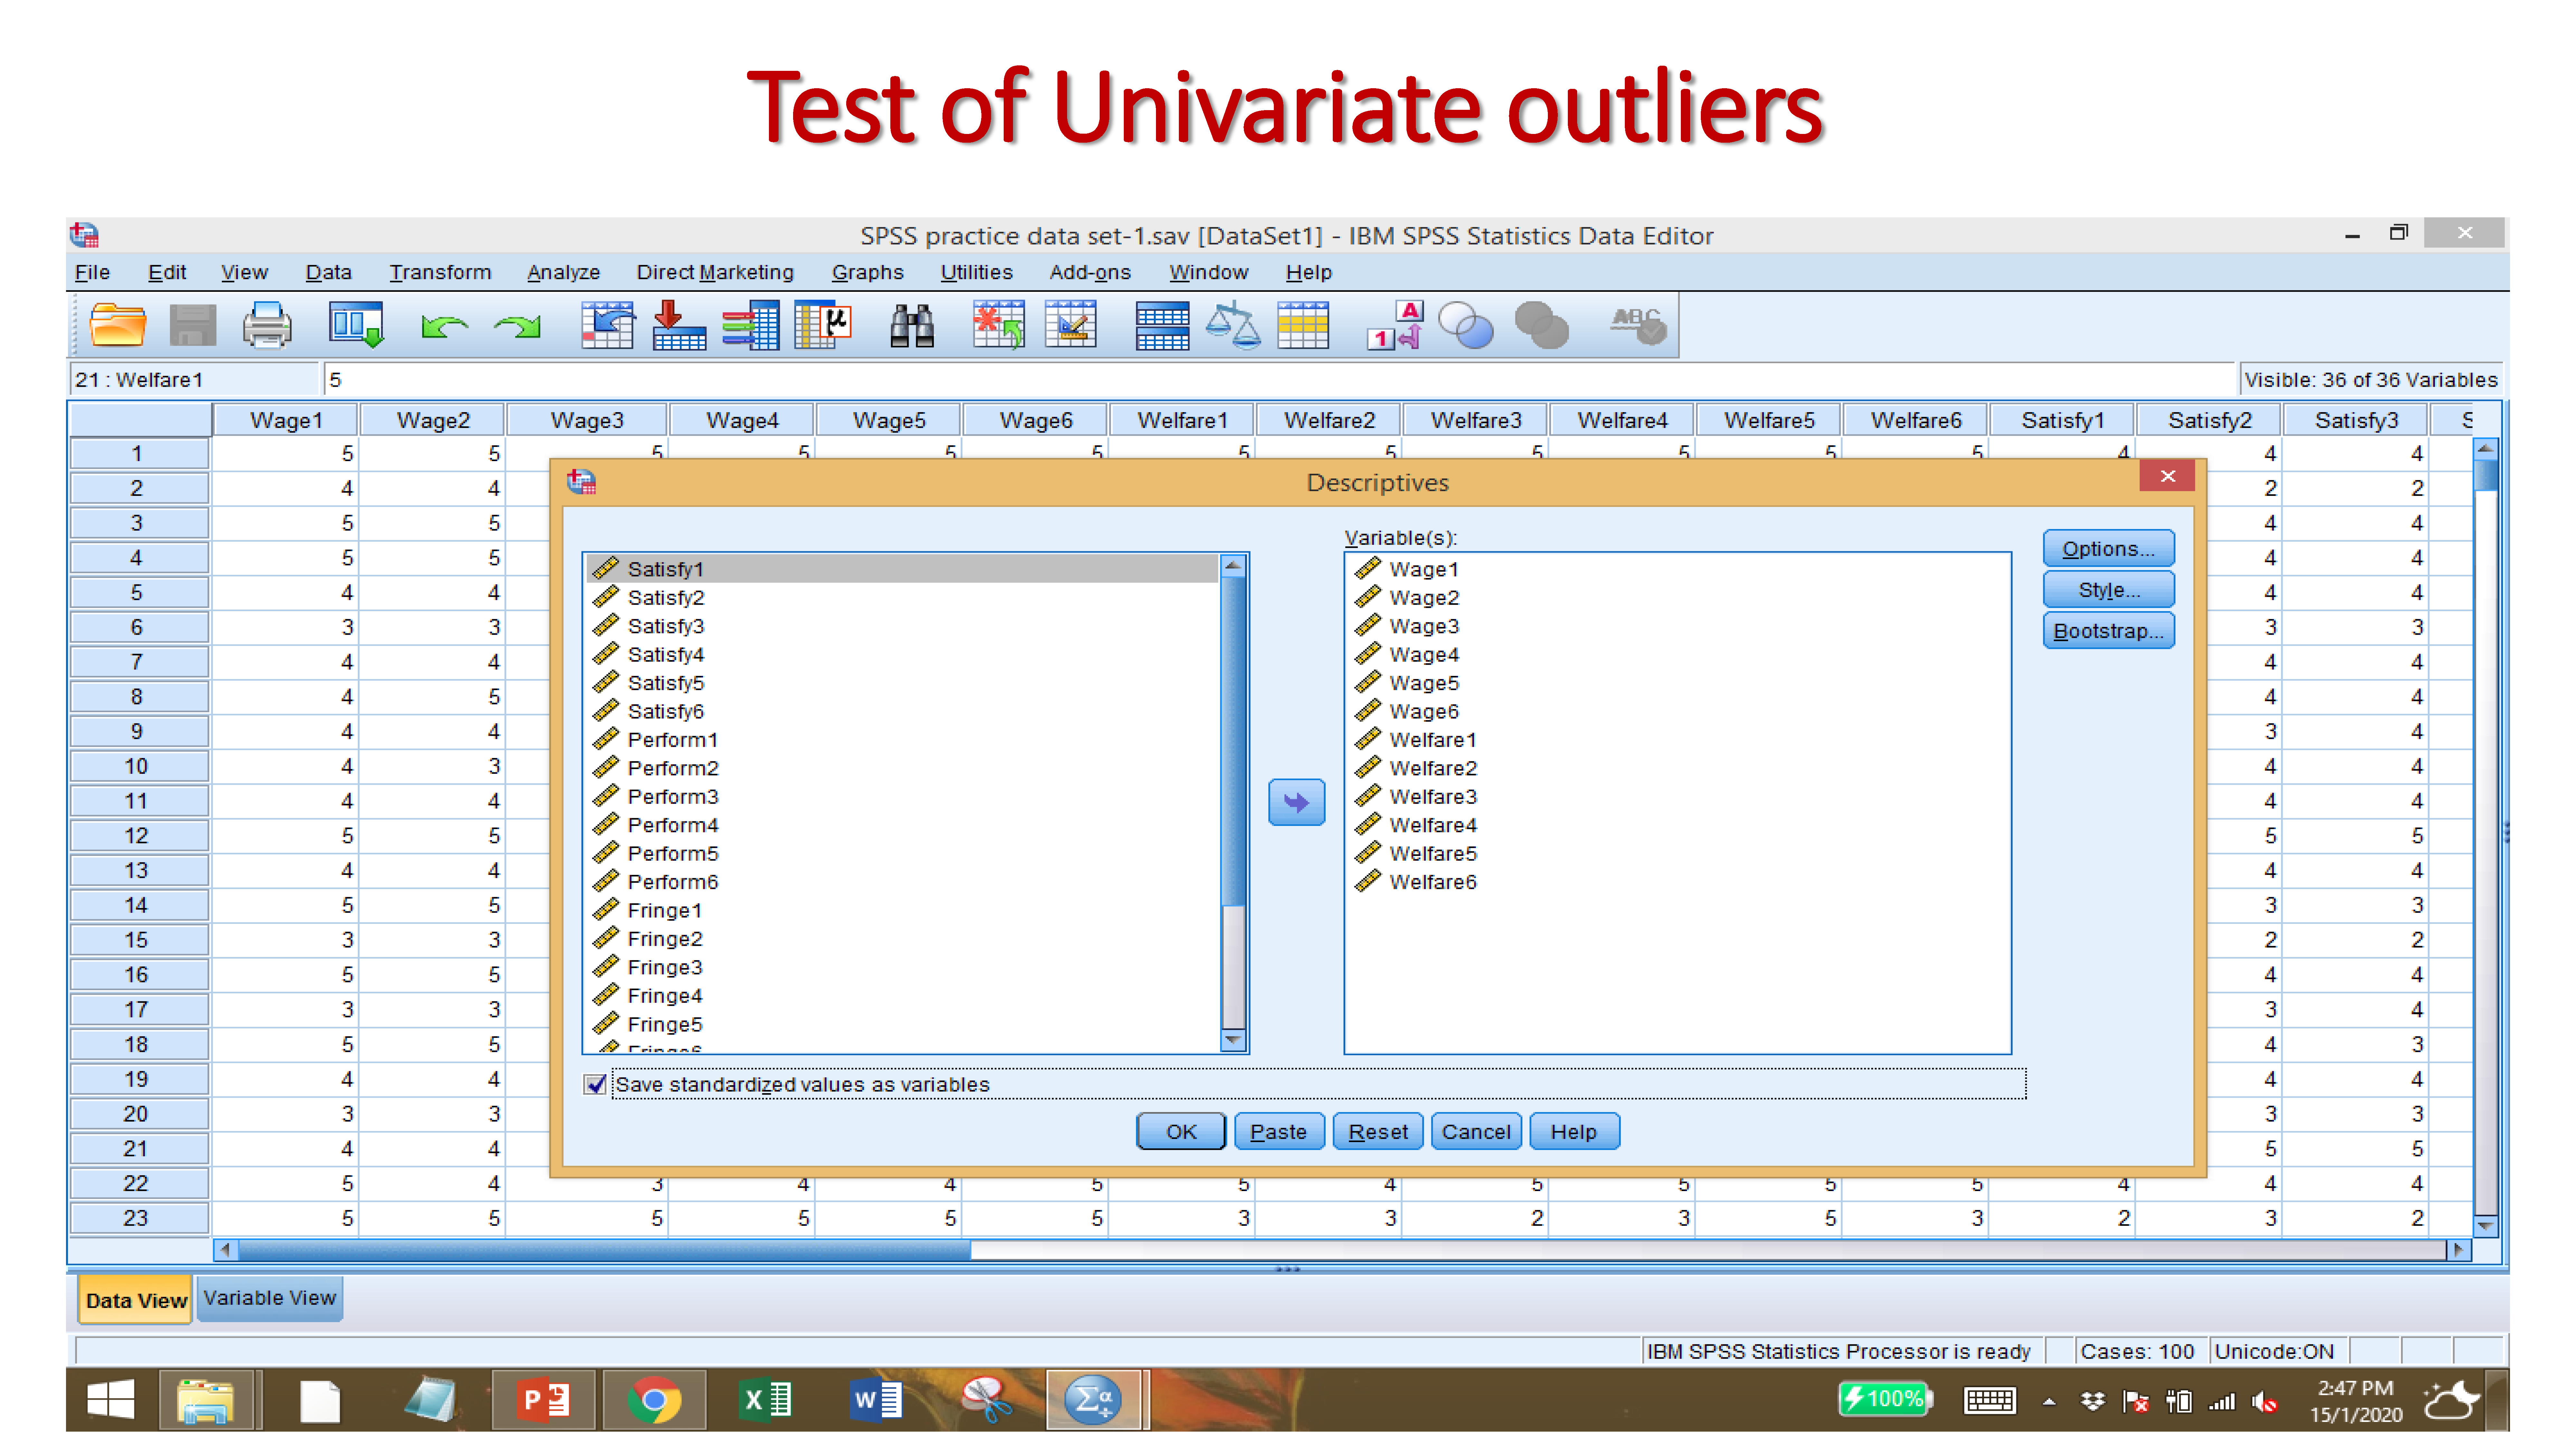
\includegraphics{images/slides/img_Page_041.png}

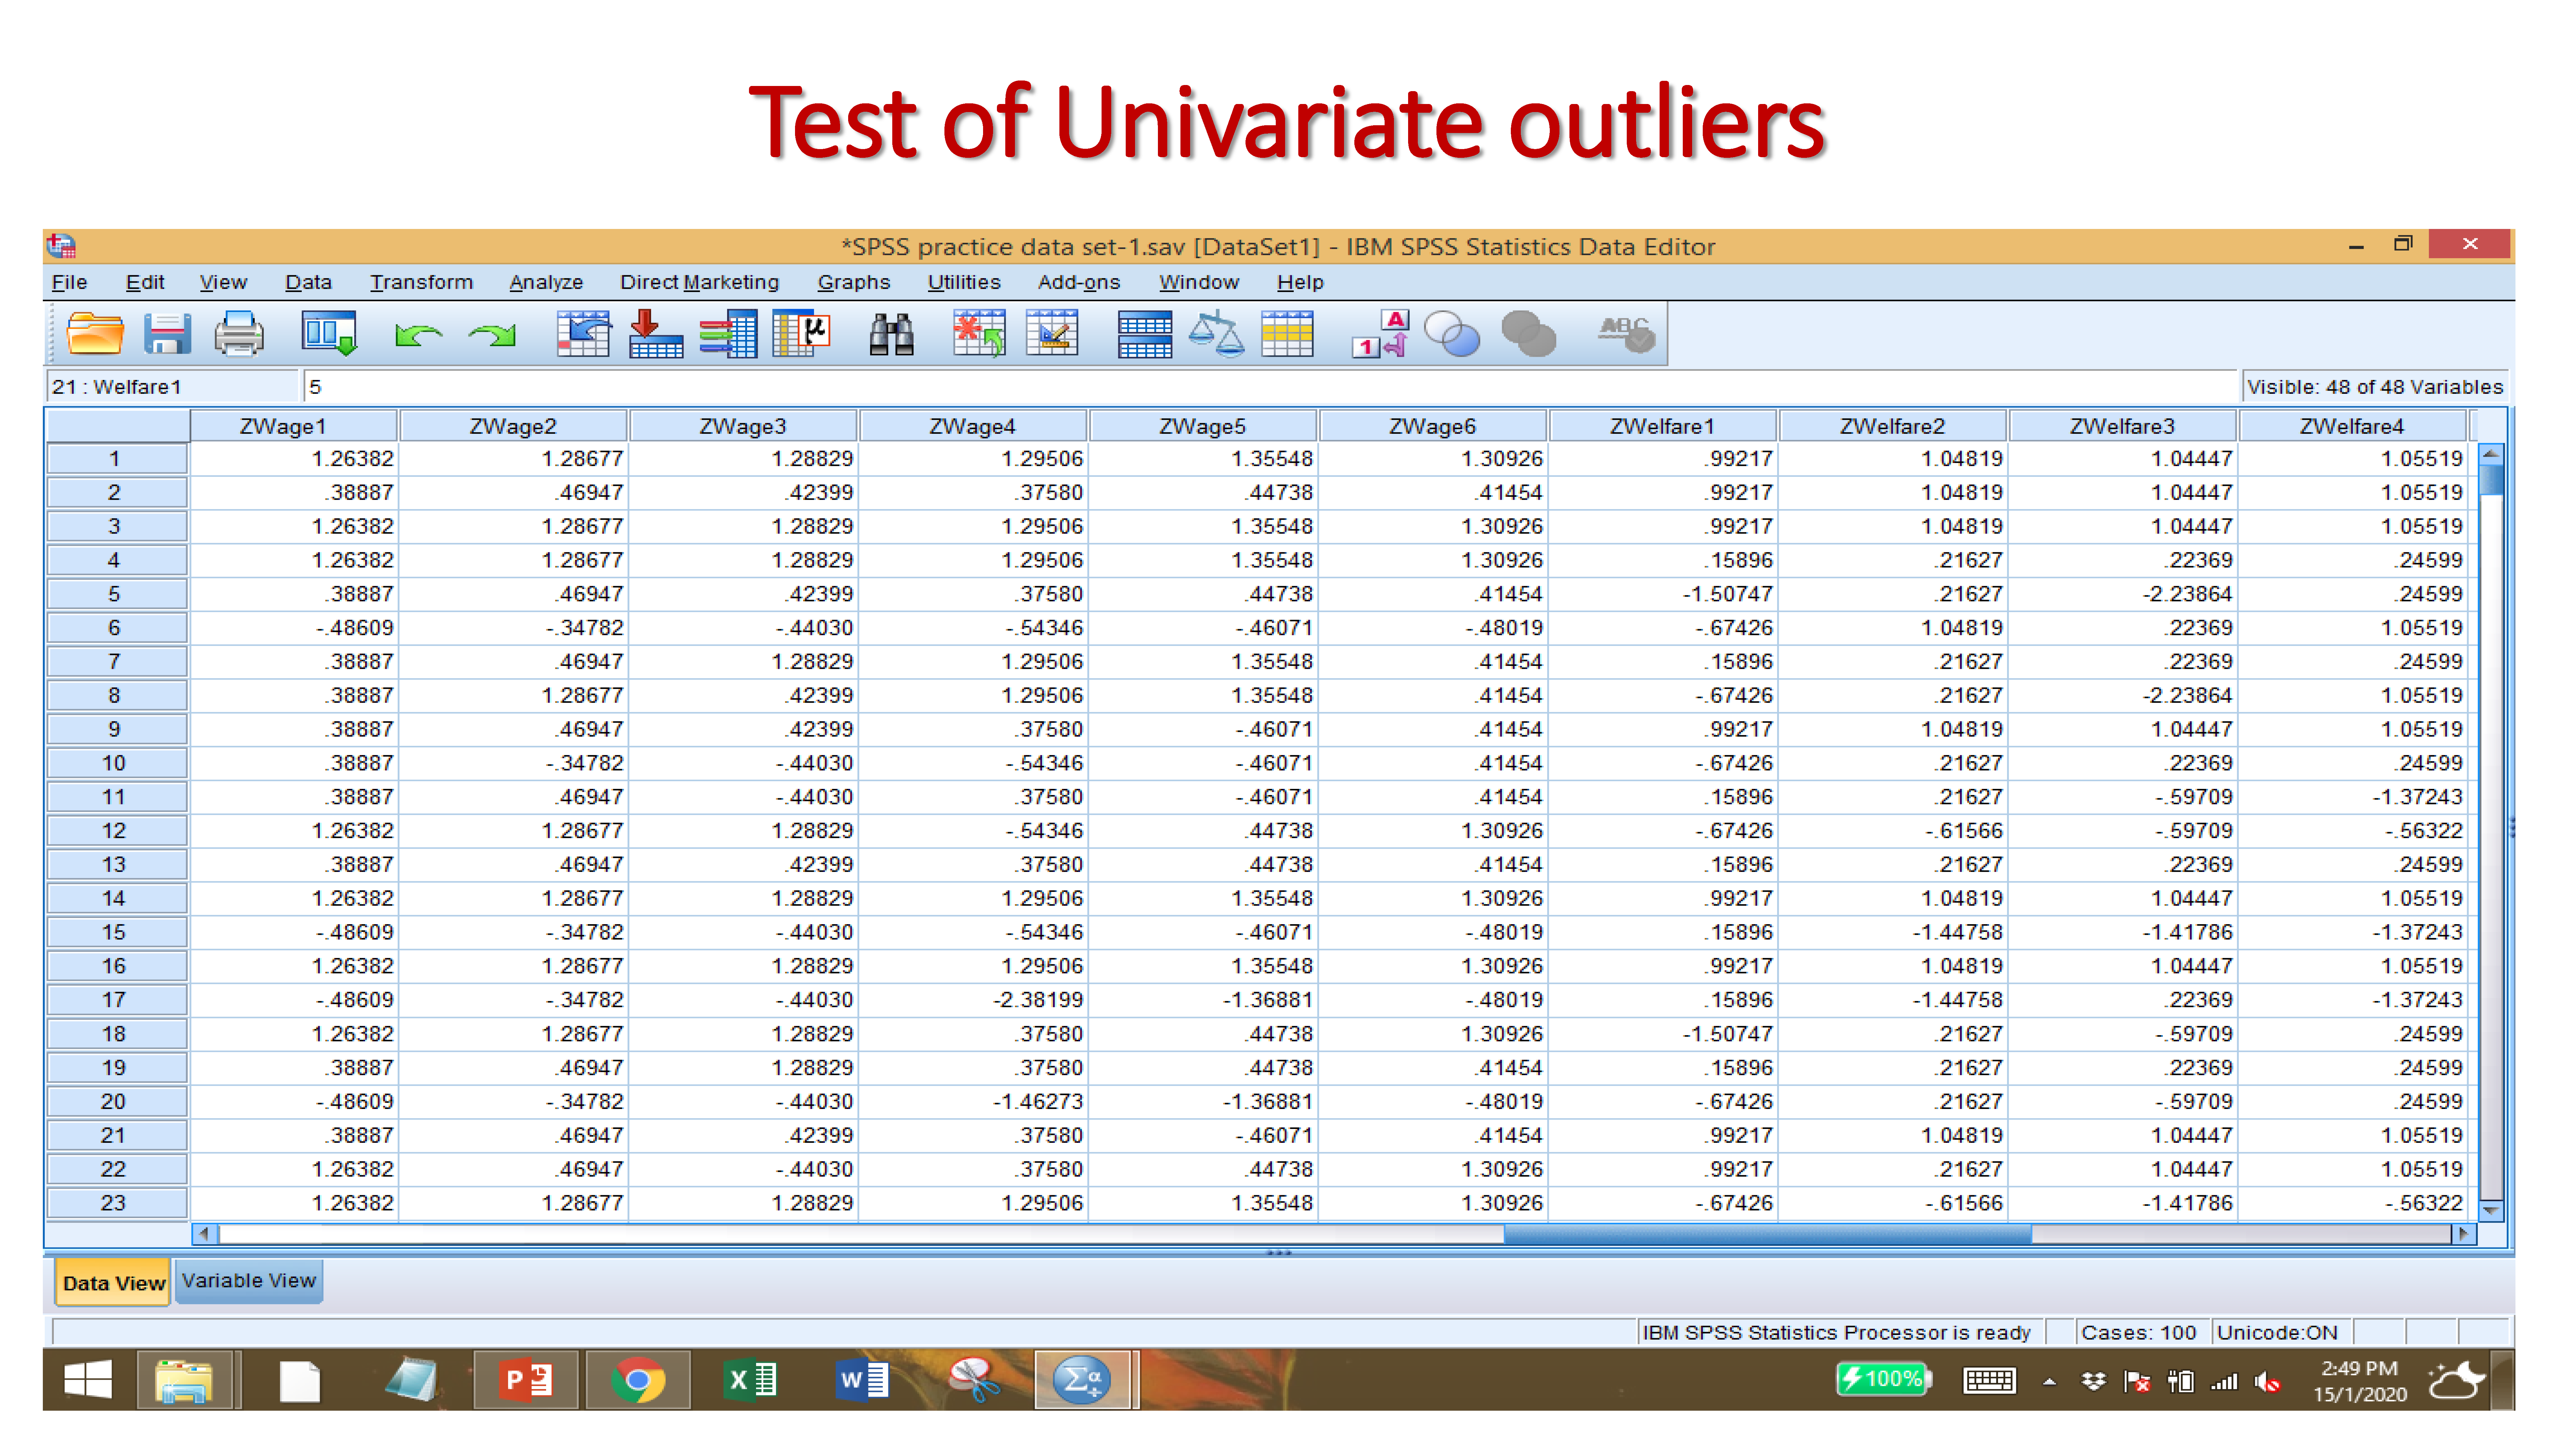
\includegraphics{images/slides/img_Page_042.png}

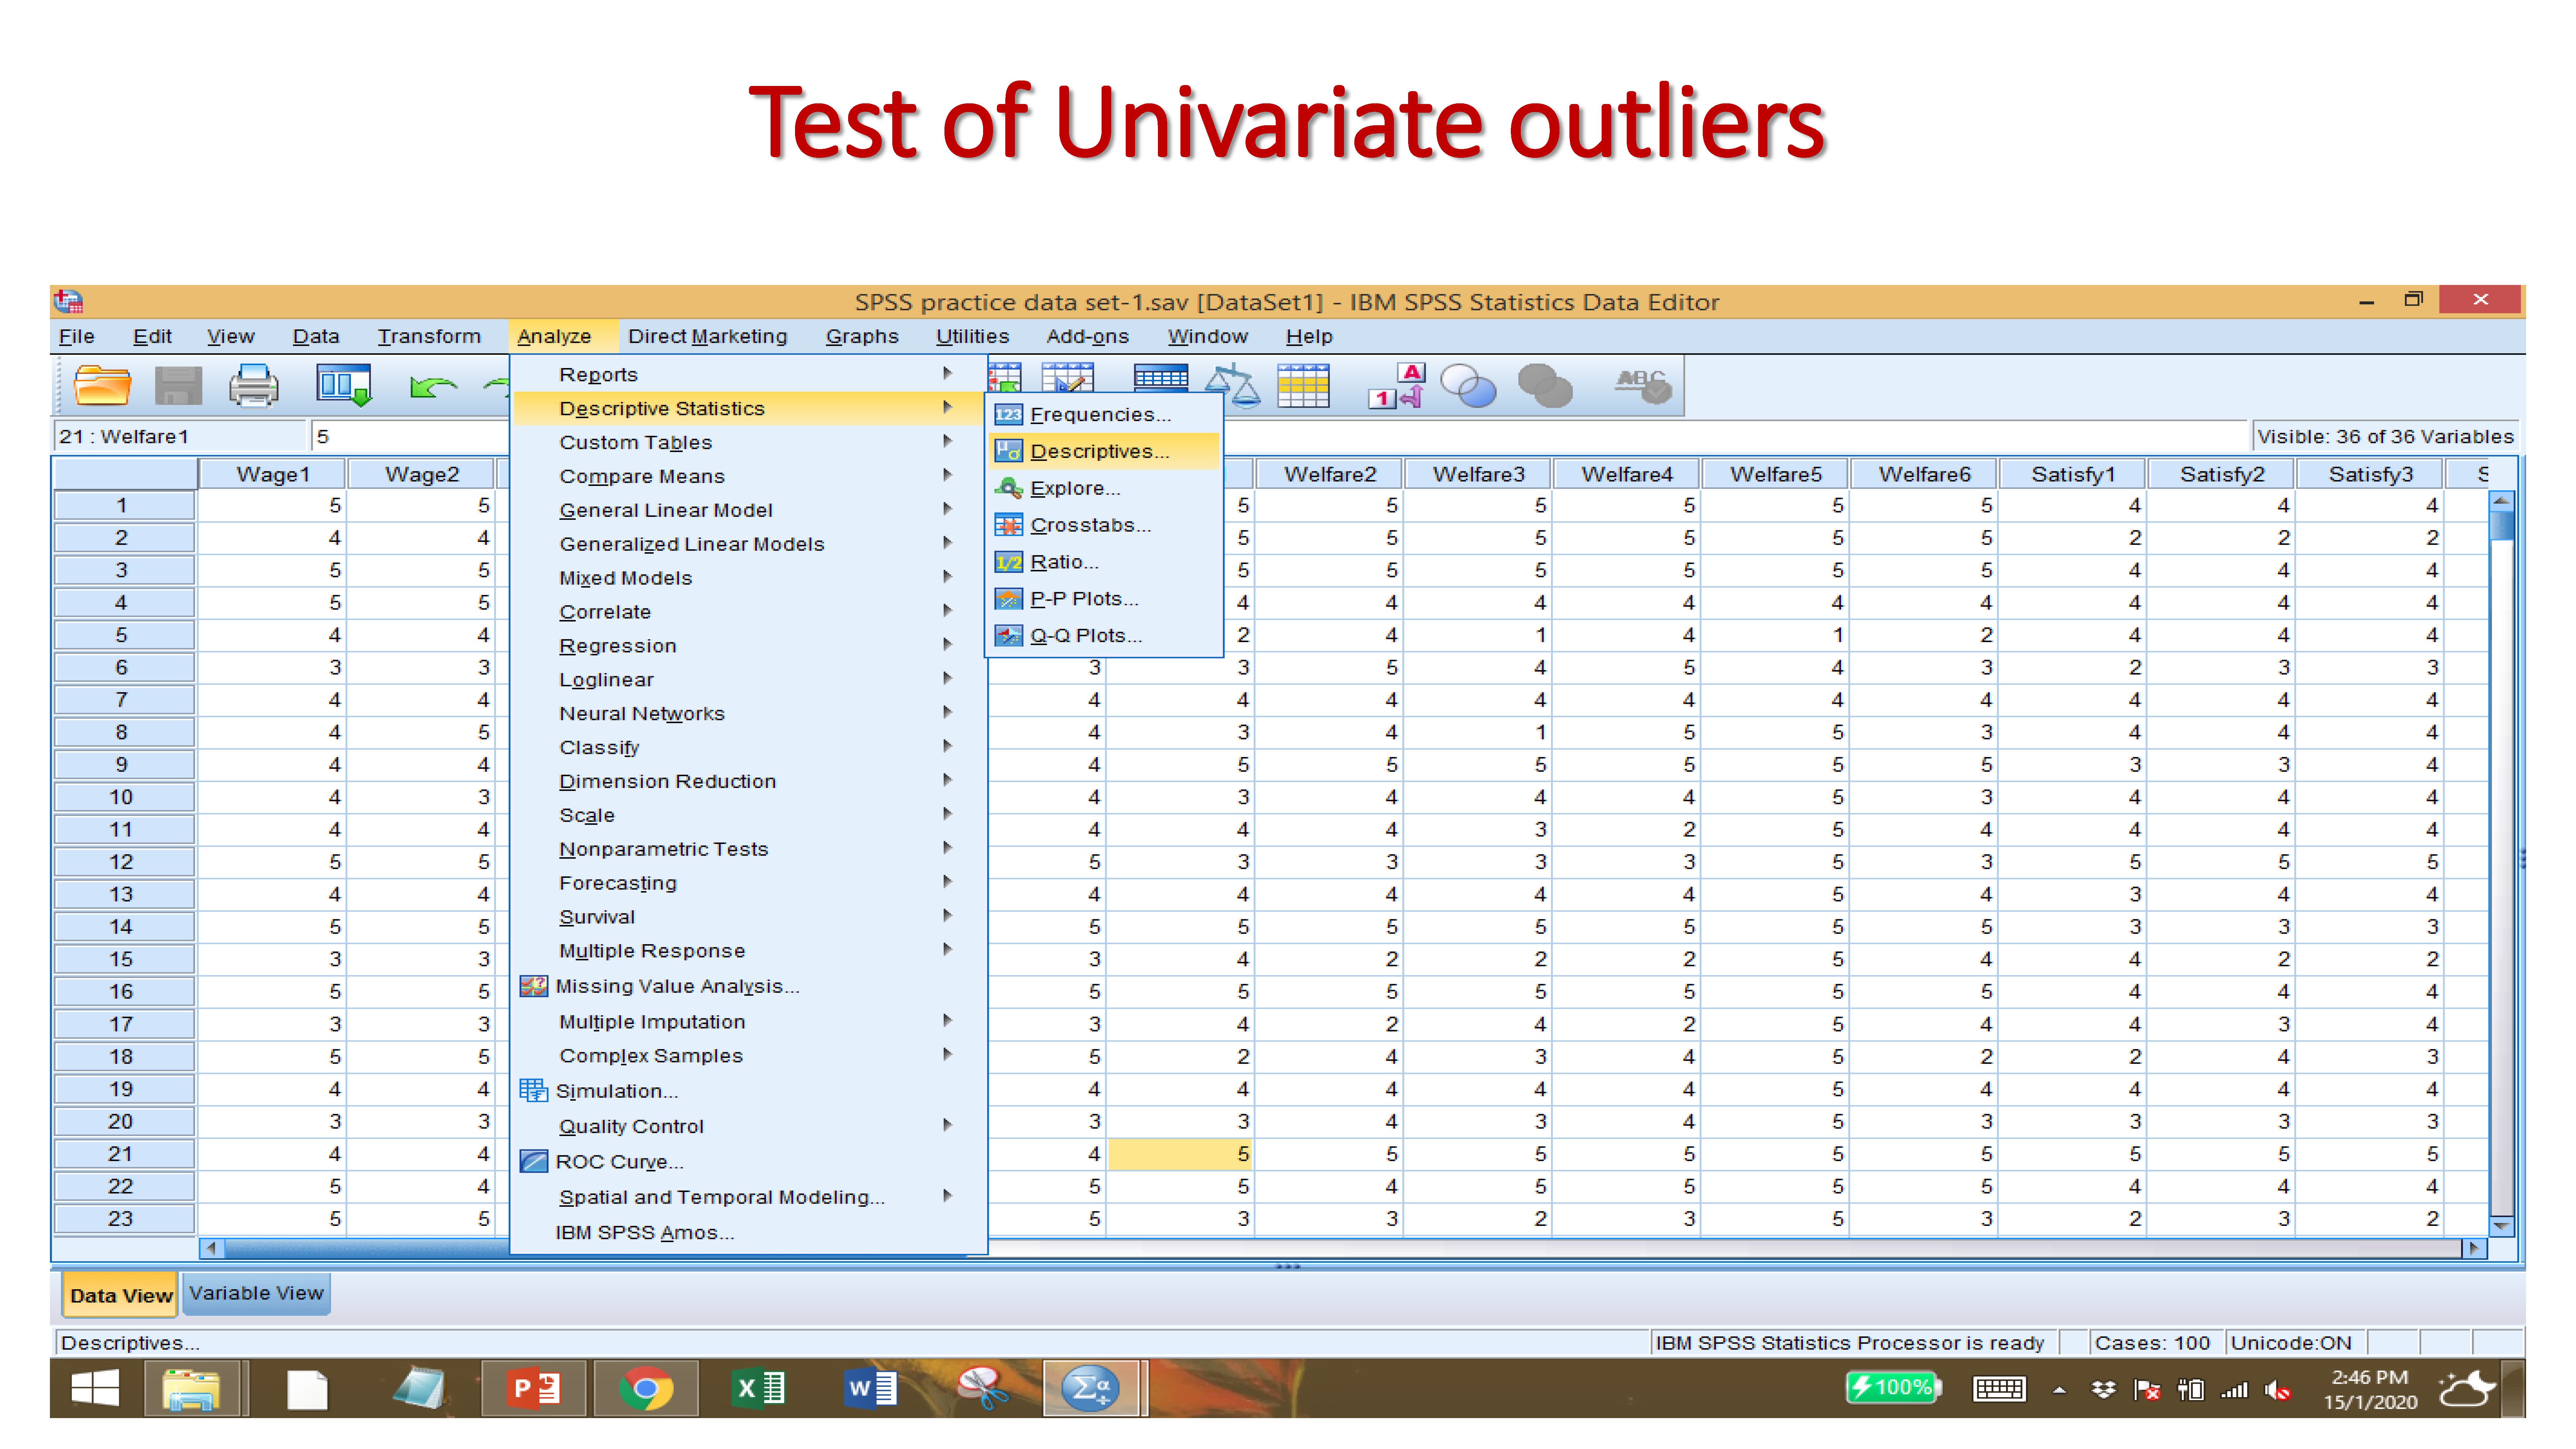
\includegraphics{images/slides/img_Page_043.png}

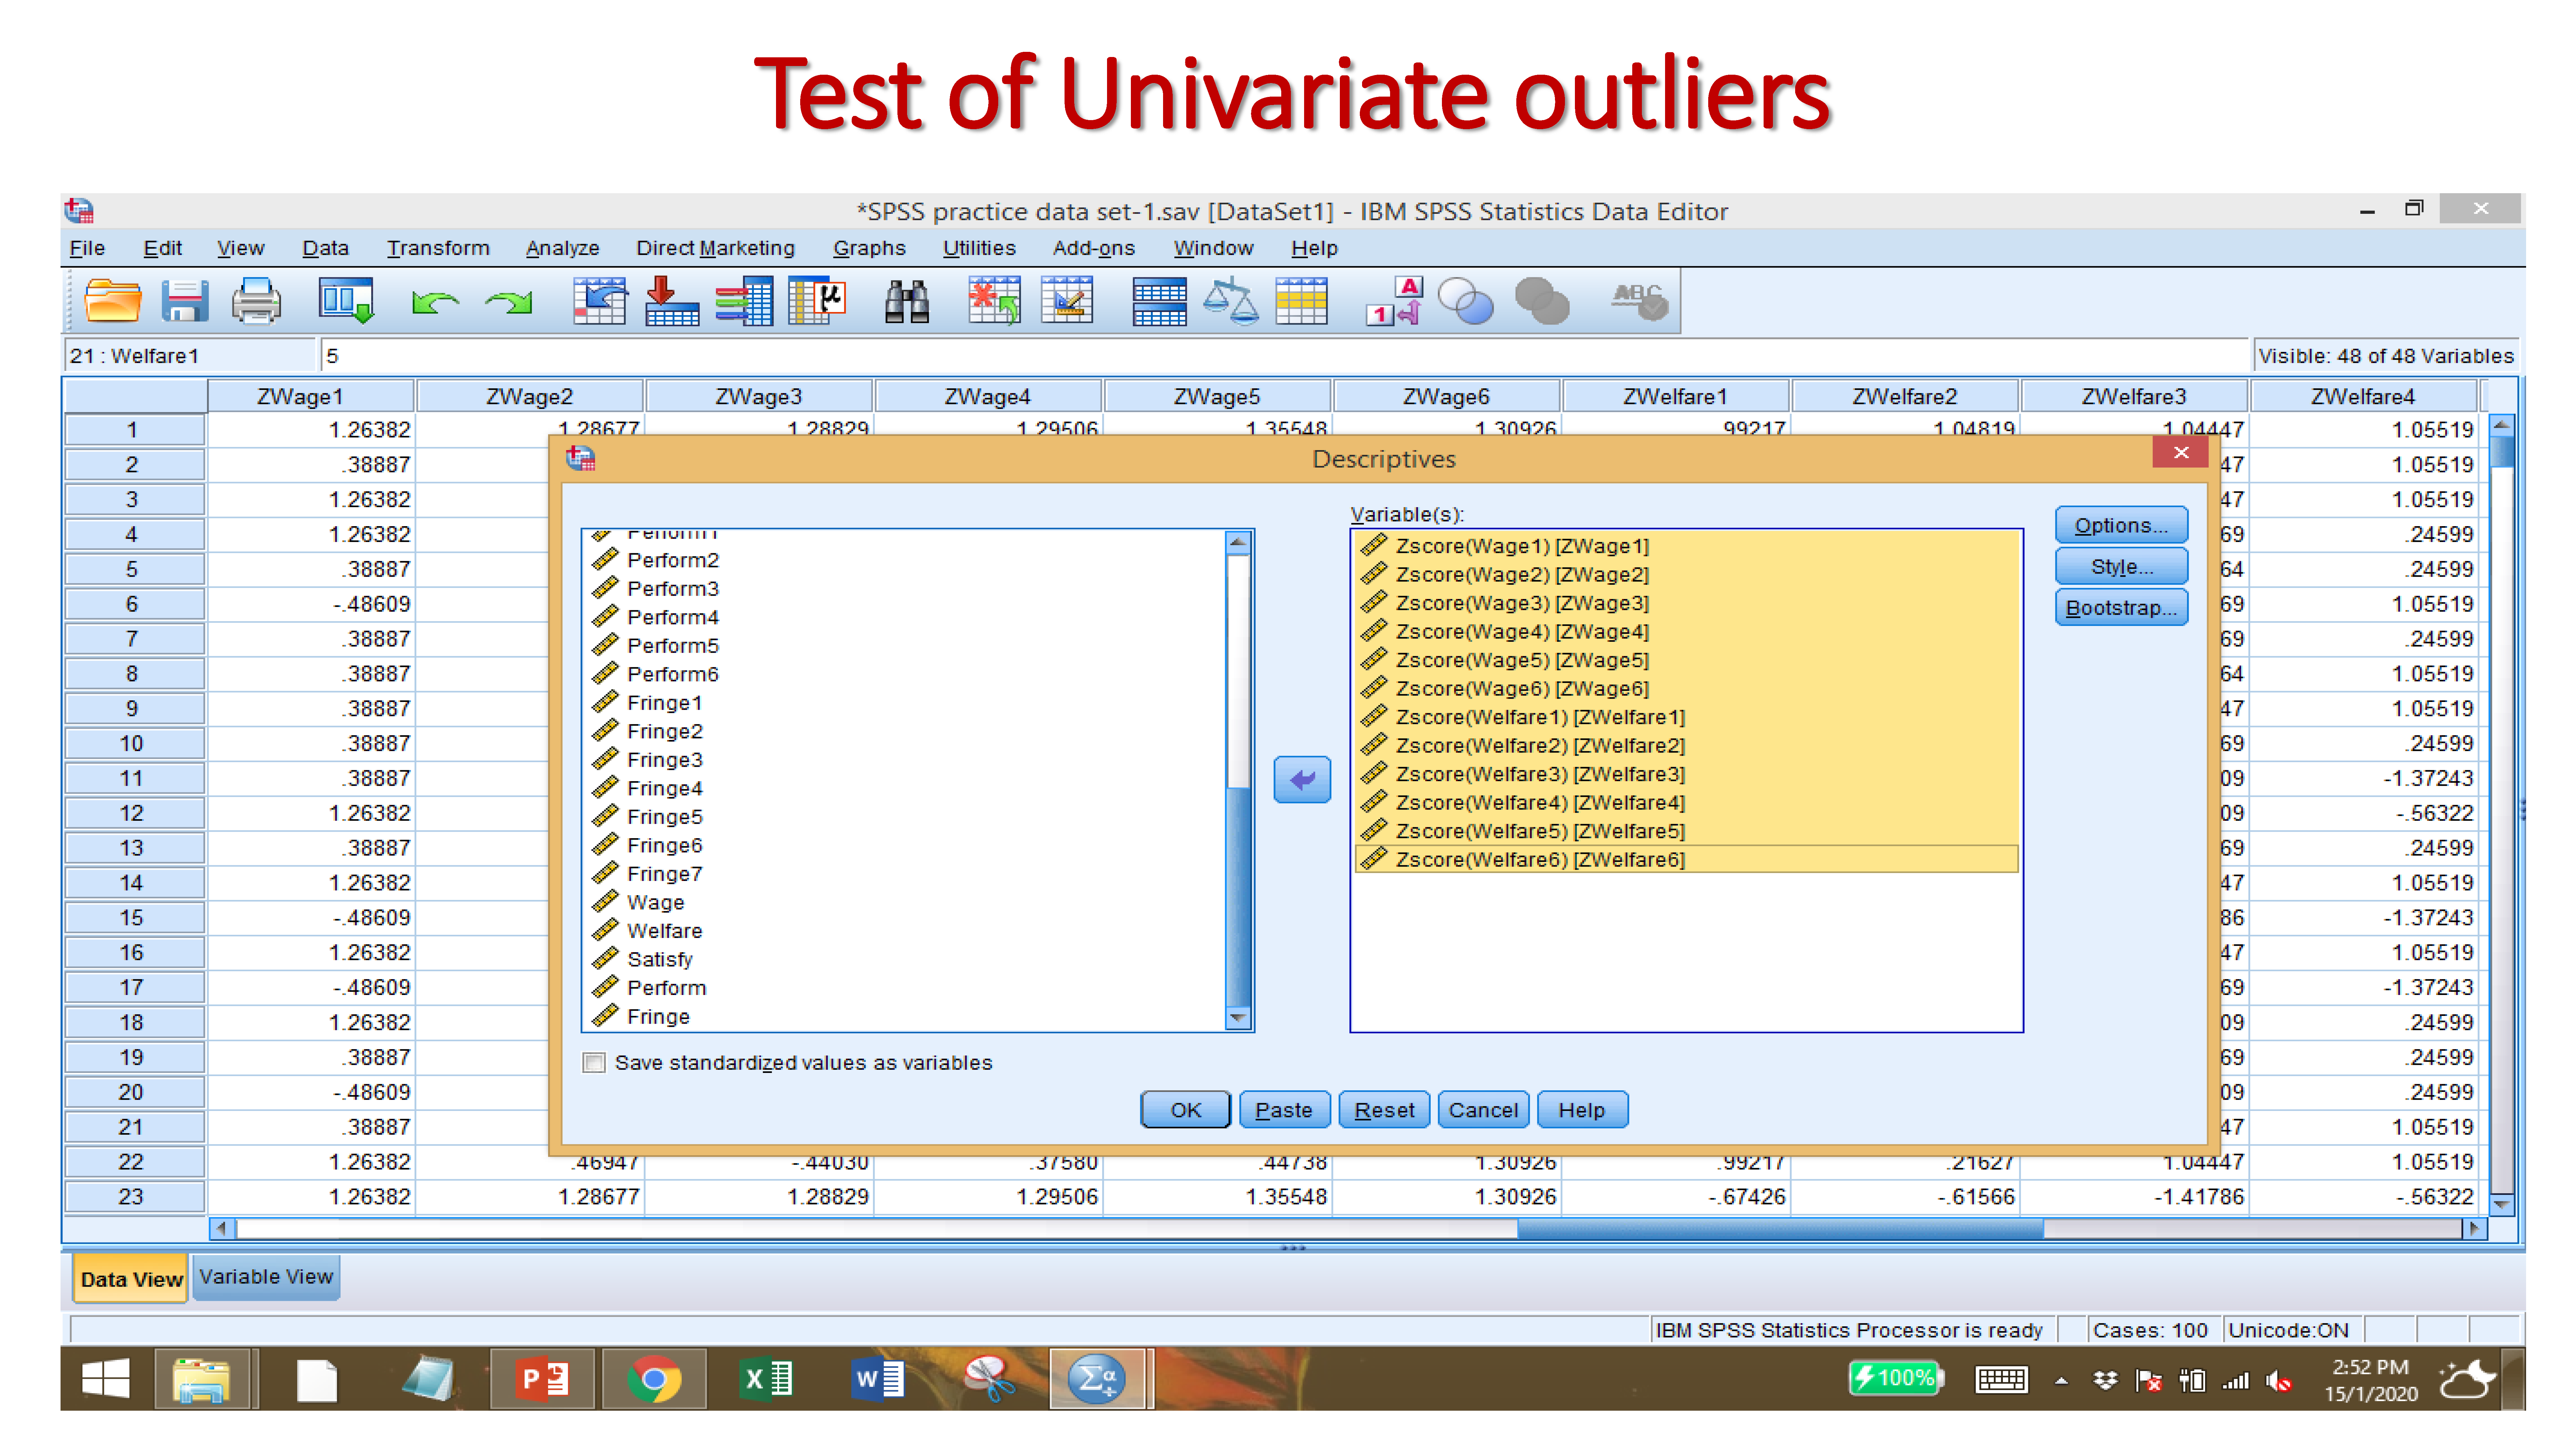
\includegraphics{images/slides/img_Page_044.png}

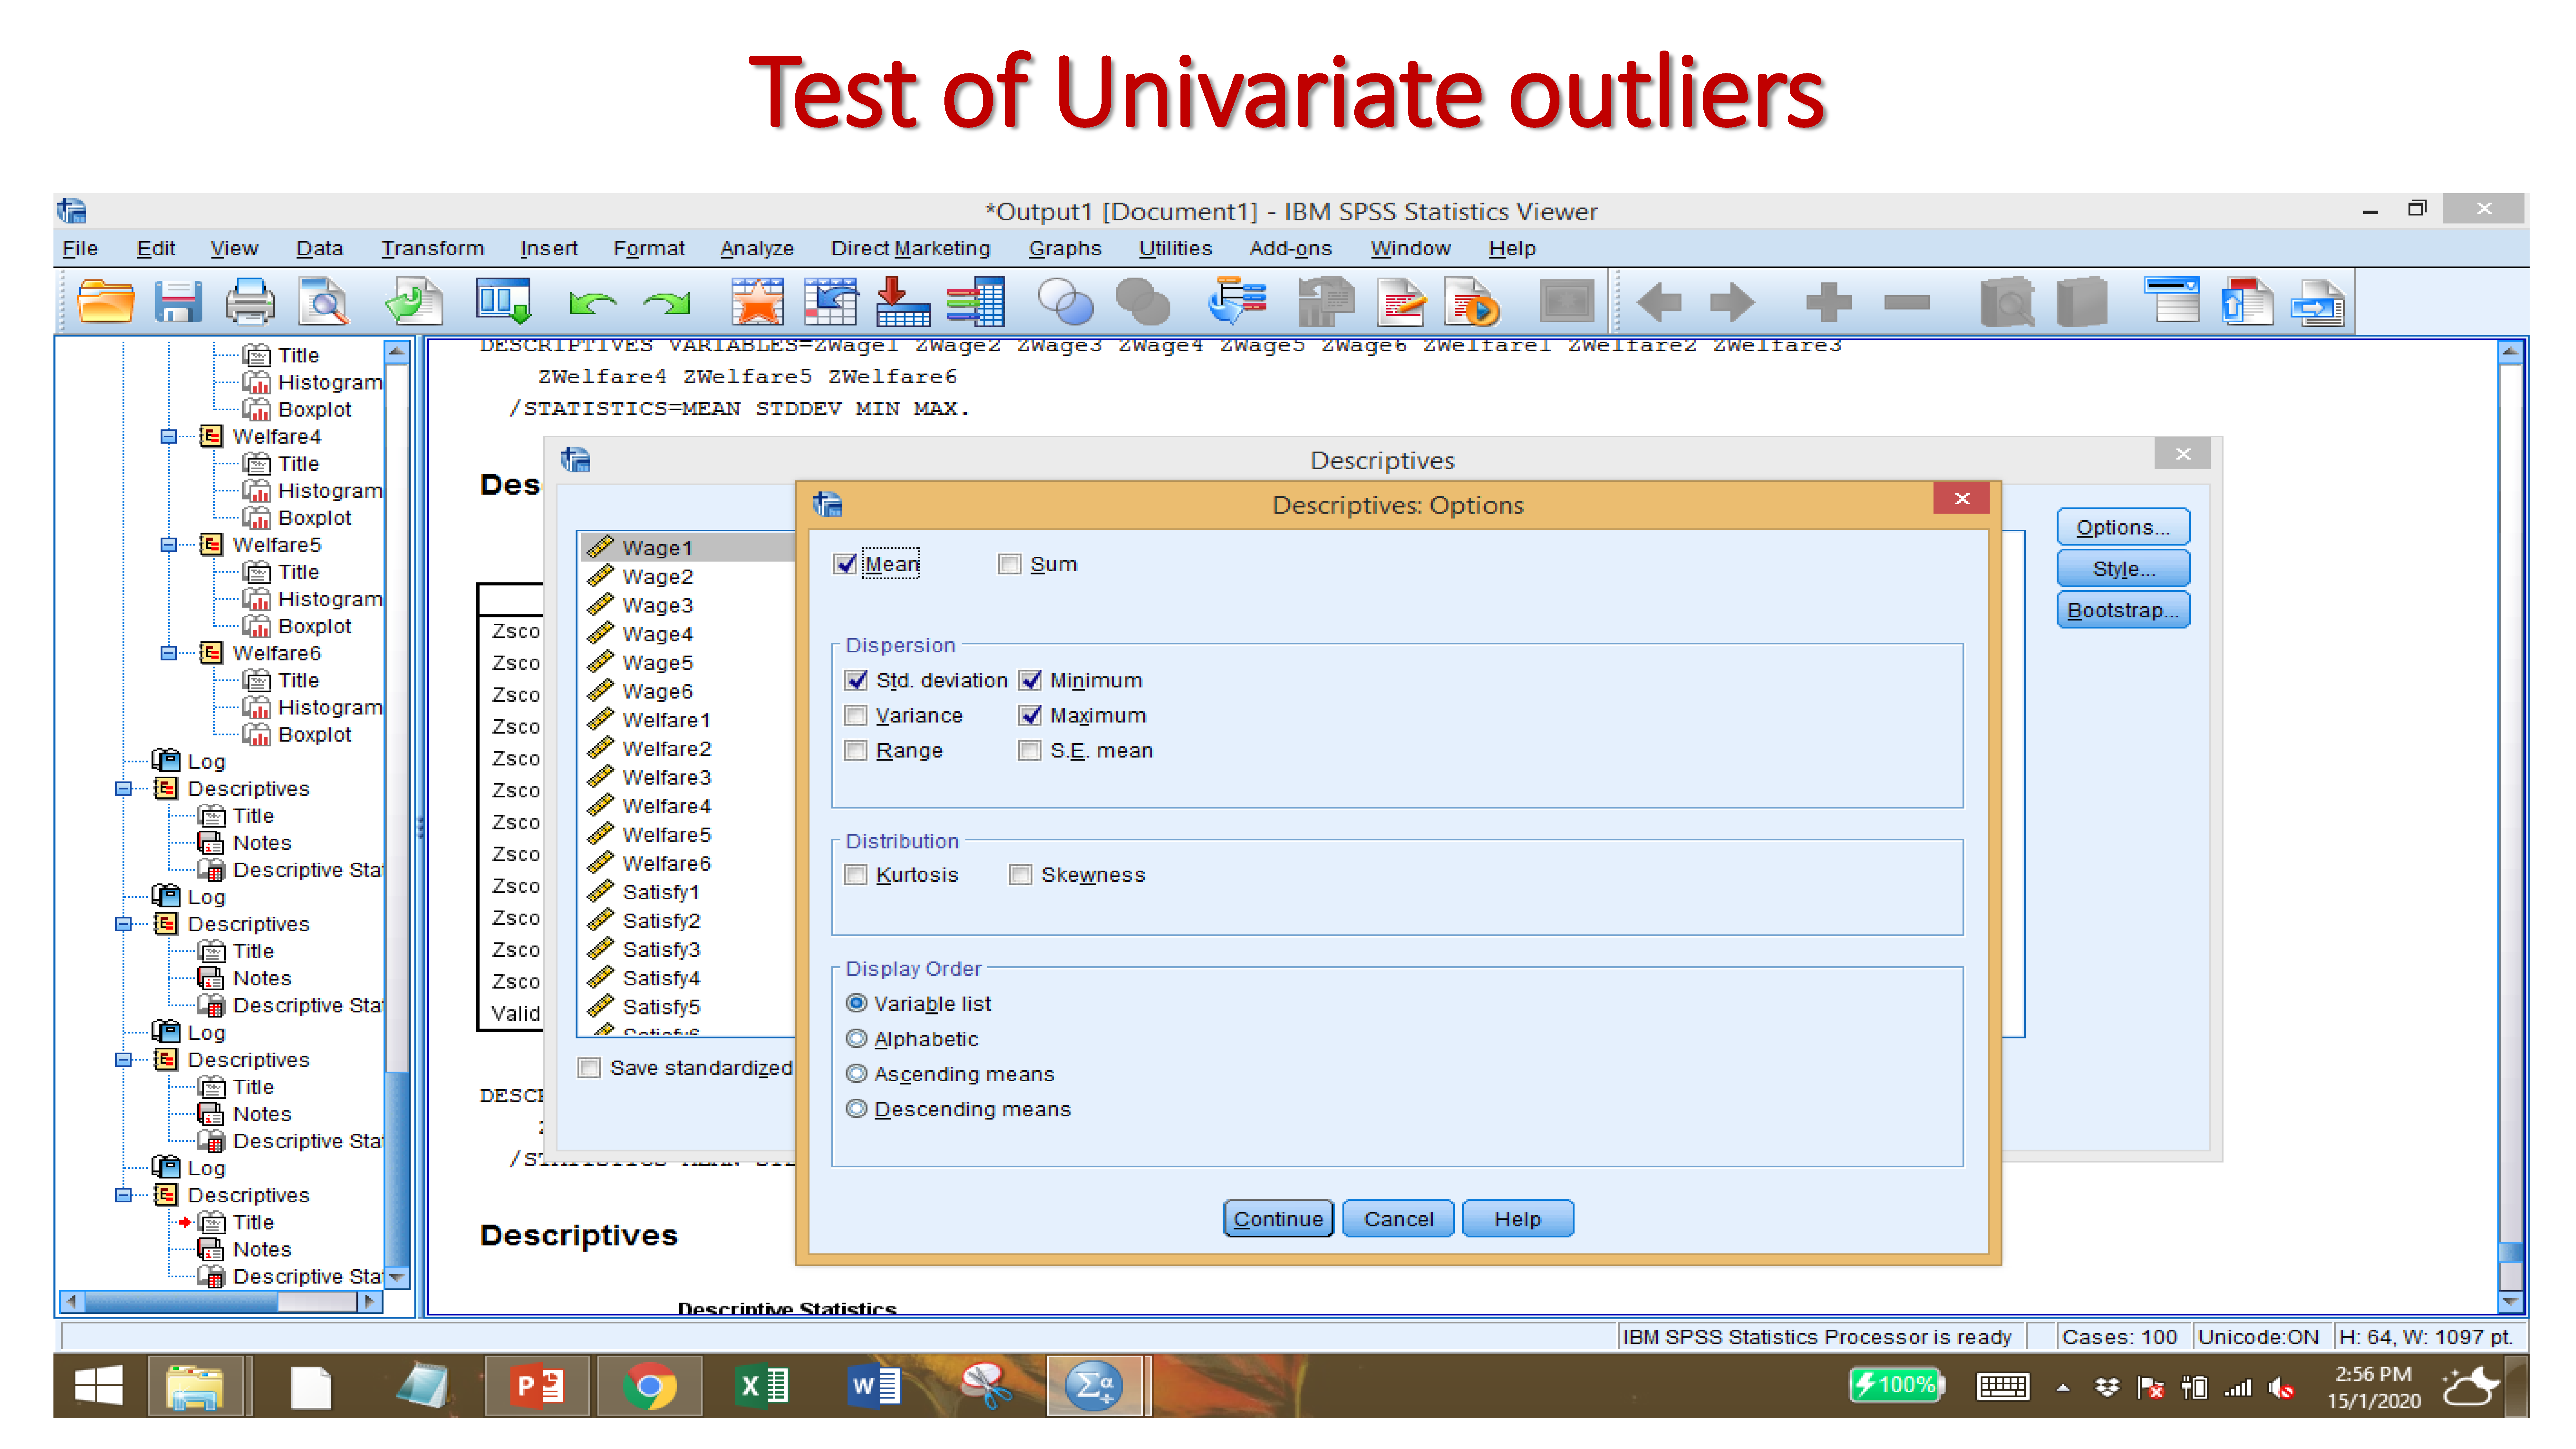
\includegraphics{images/slides/img_Page_045.png}

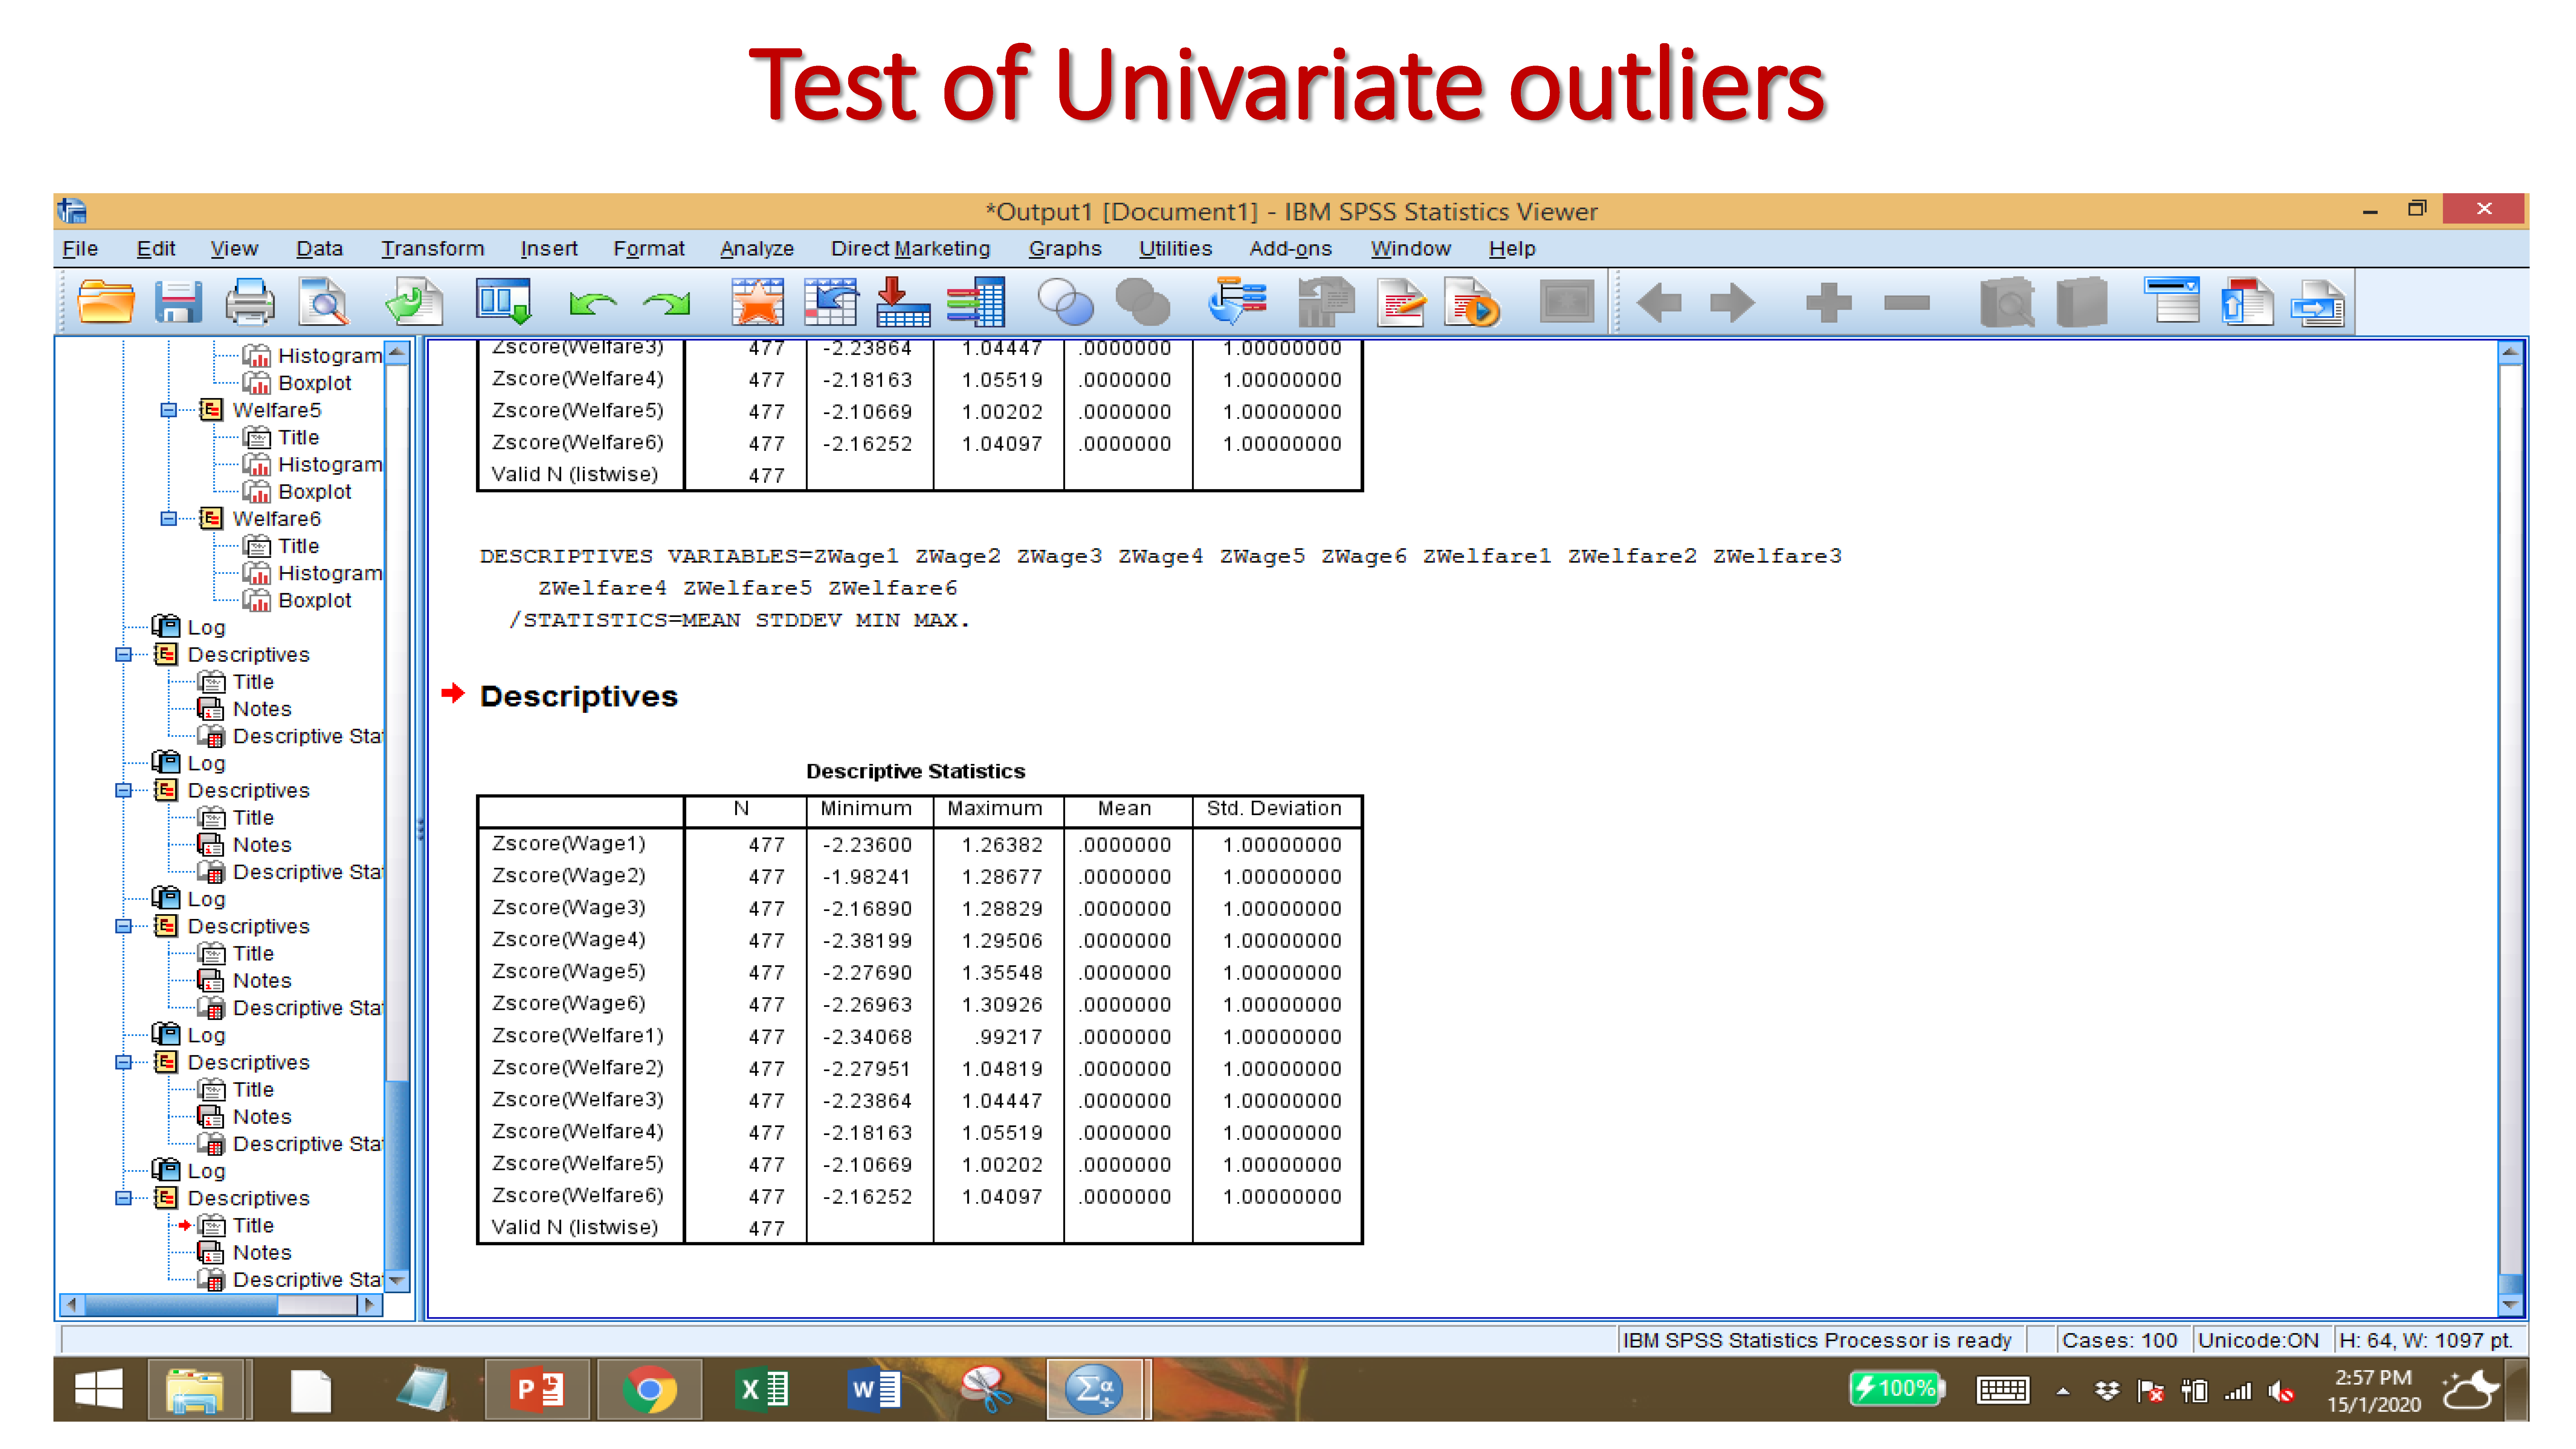
\includegraphics{images/slides/img_Page_046.png}

\begin{tcolorbox}[enhanced jigsaw, rightrule=.15mm, arc=.35mm, colframe=quarto-callout-note-color-frame, coltitle=black, left=2mm, colbacktitle=quarto-callout-note-color!10!white, bottomtitle=1mm, titlerule=0mm, colback=white, breakable, opacitybacktitle=0.6, opacityback=0, toprule=.15mm, toptitle=1mm, title=\textcolor{quarto-callout-note-color}{\faInfo}\hspace{0.5em}{Univariate outliers criterion}, bottomrule=.15mm, leftrule=.75mm]

If the Z-Score Value beyond the value +3.29 to -3.29 for a large sample
size (more than 80) then there is outliers. If the Z-Score Value beyond
the value +2.50 to -2.50 for the case of small sample size (less than 80
samples) then there is outliers.

\end{tcolorbox}

\section{Test of multivariate
outliers}\label{test-of-multivariate-outliers}

A multivariate outlier is a combination of unusual scores on at least
two variables. Both types of outliers can influence the outcome of
statistical analyses. The multivariate outliers can be identified by the
test of\\

\begin{itemize}
\tightlist
\item
  Mahalanobis Distance
\end{itemize}

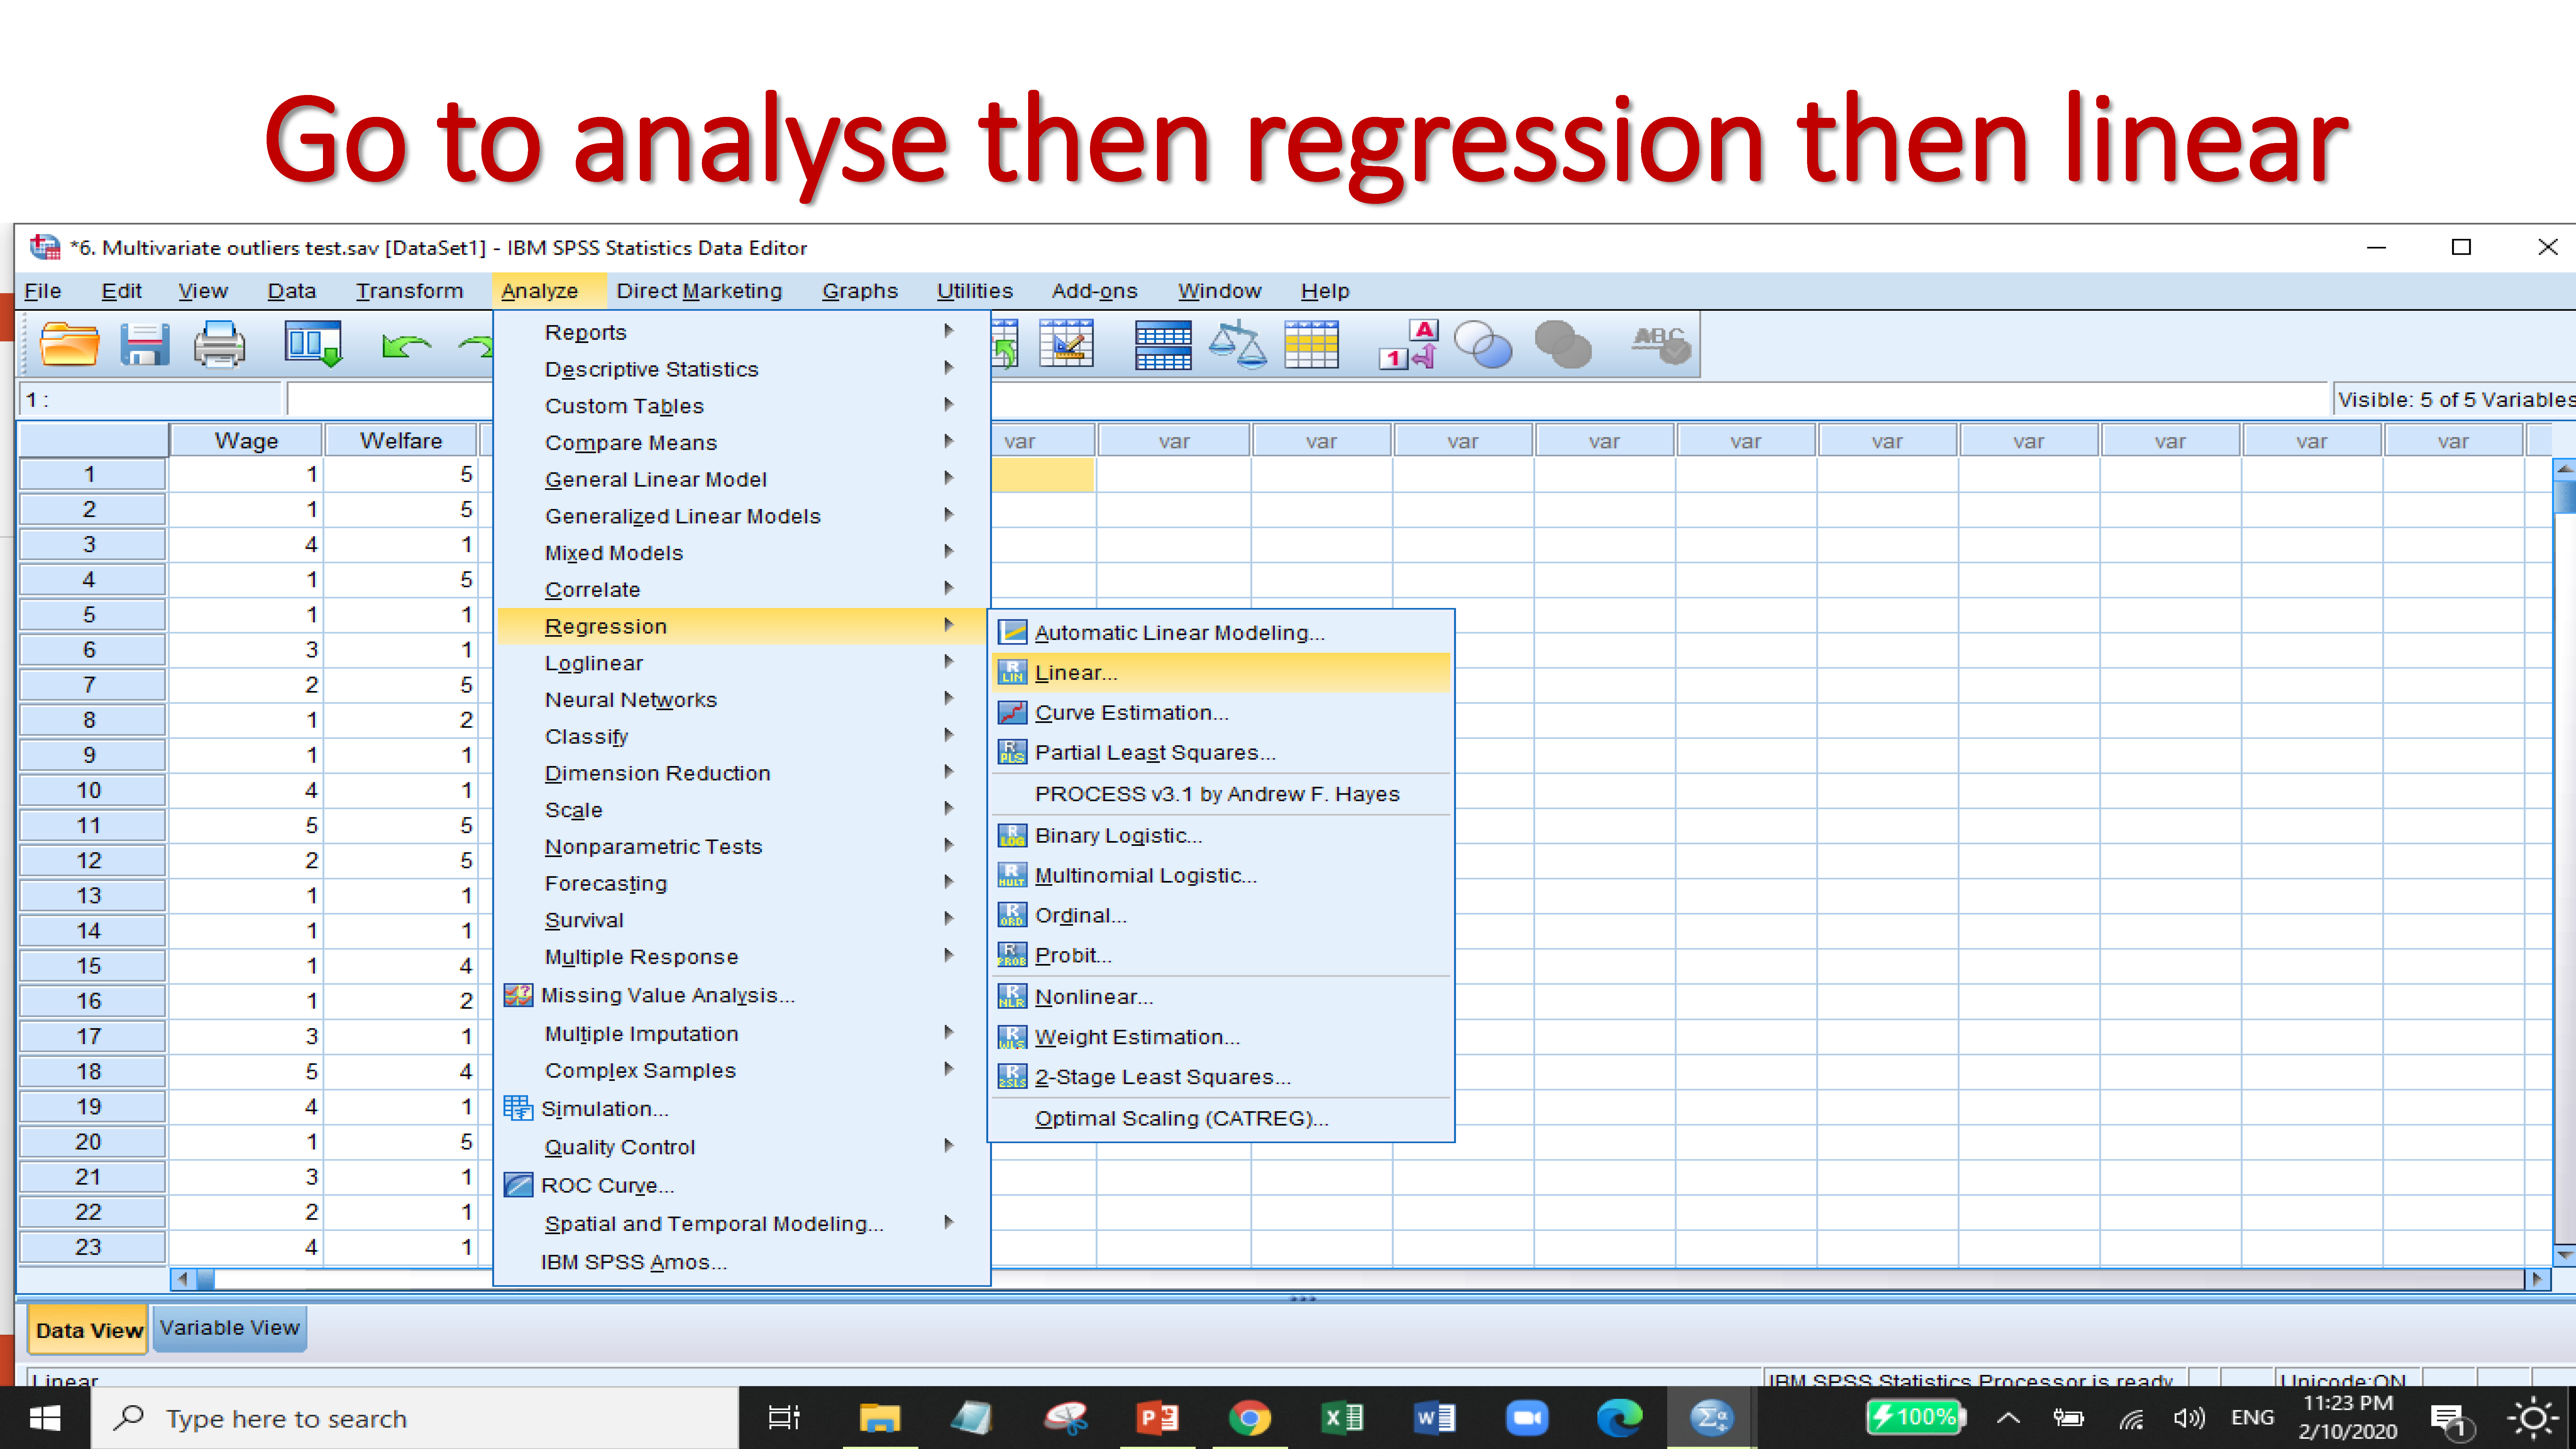
\includegraphics{images/slides/img_Page_049.png}

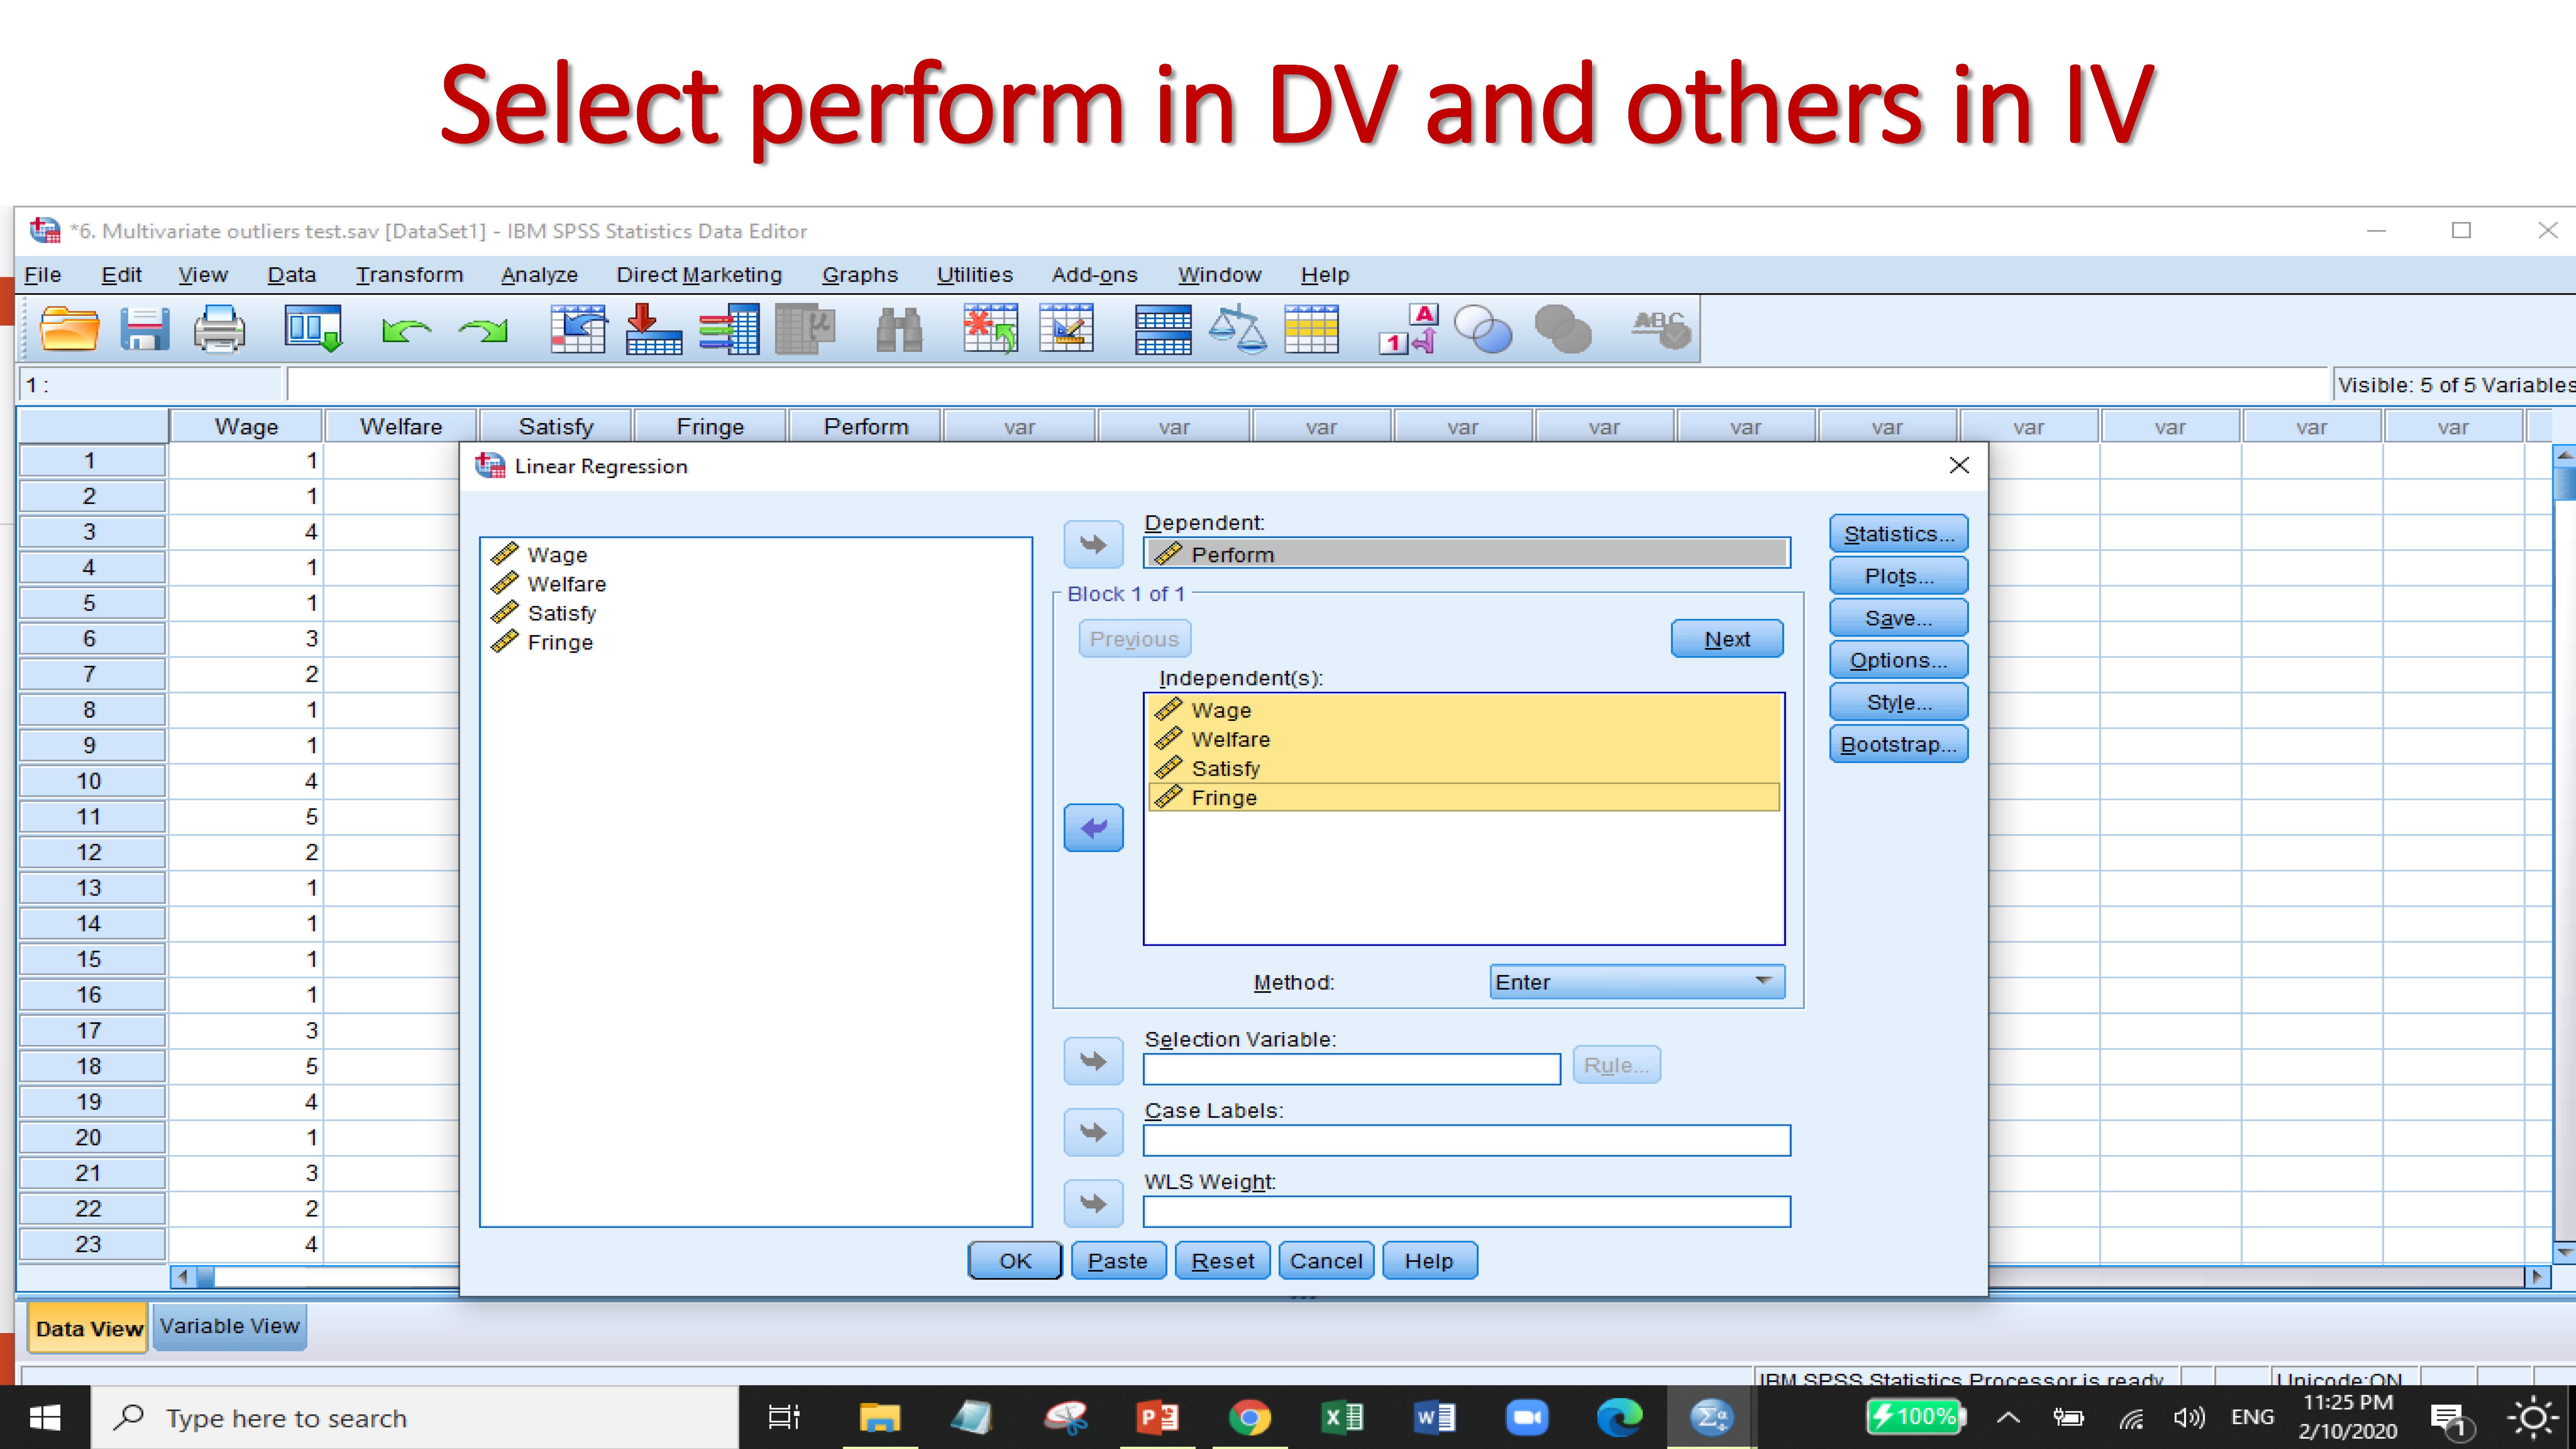
\includegraphics{images/slides/img_Page_050.png}

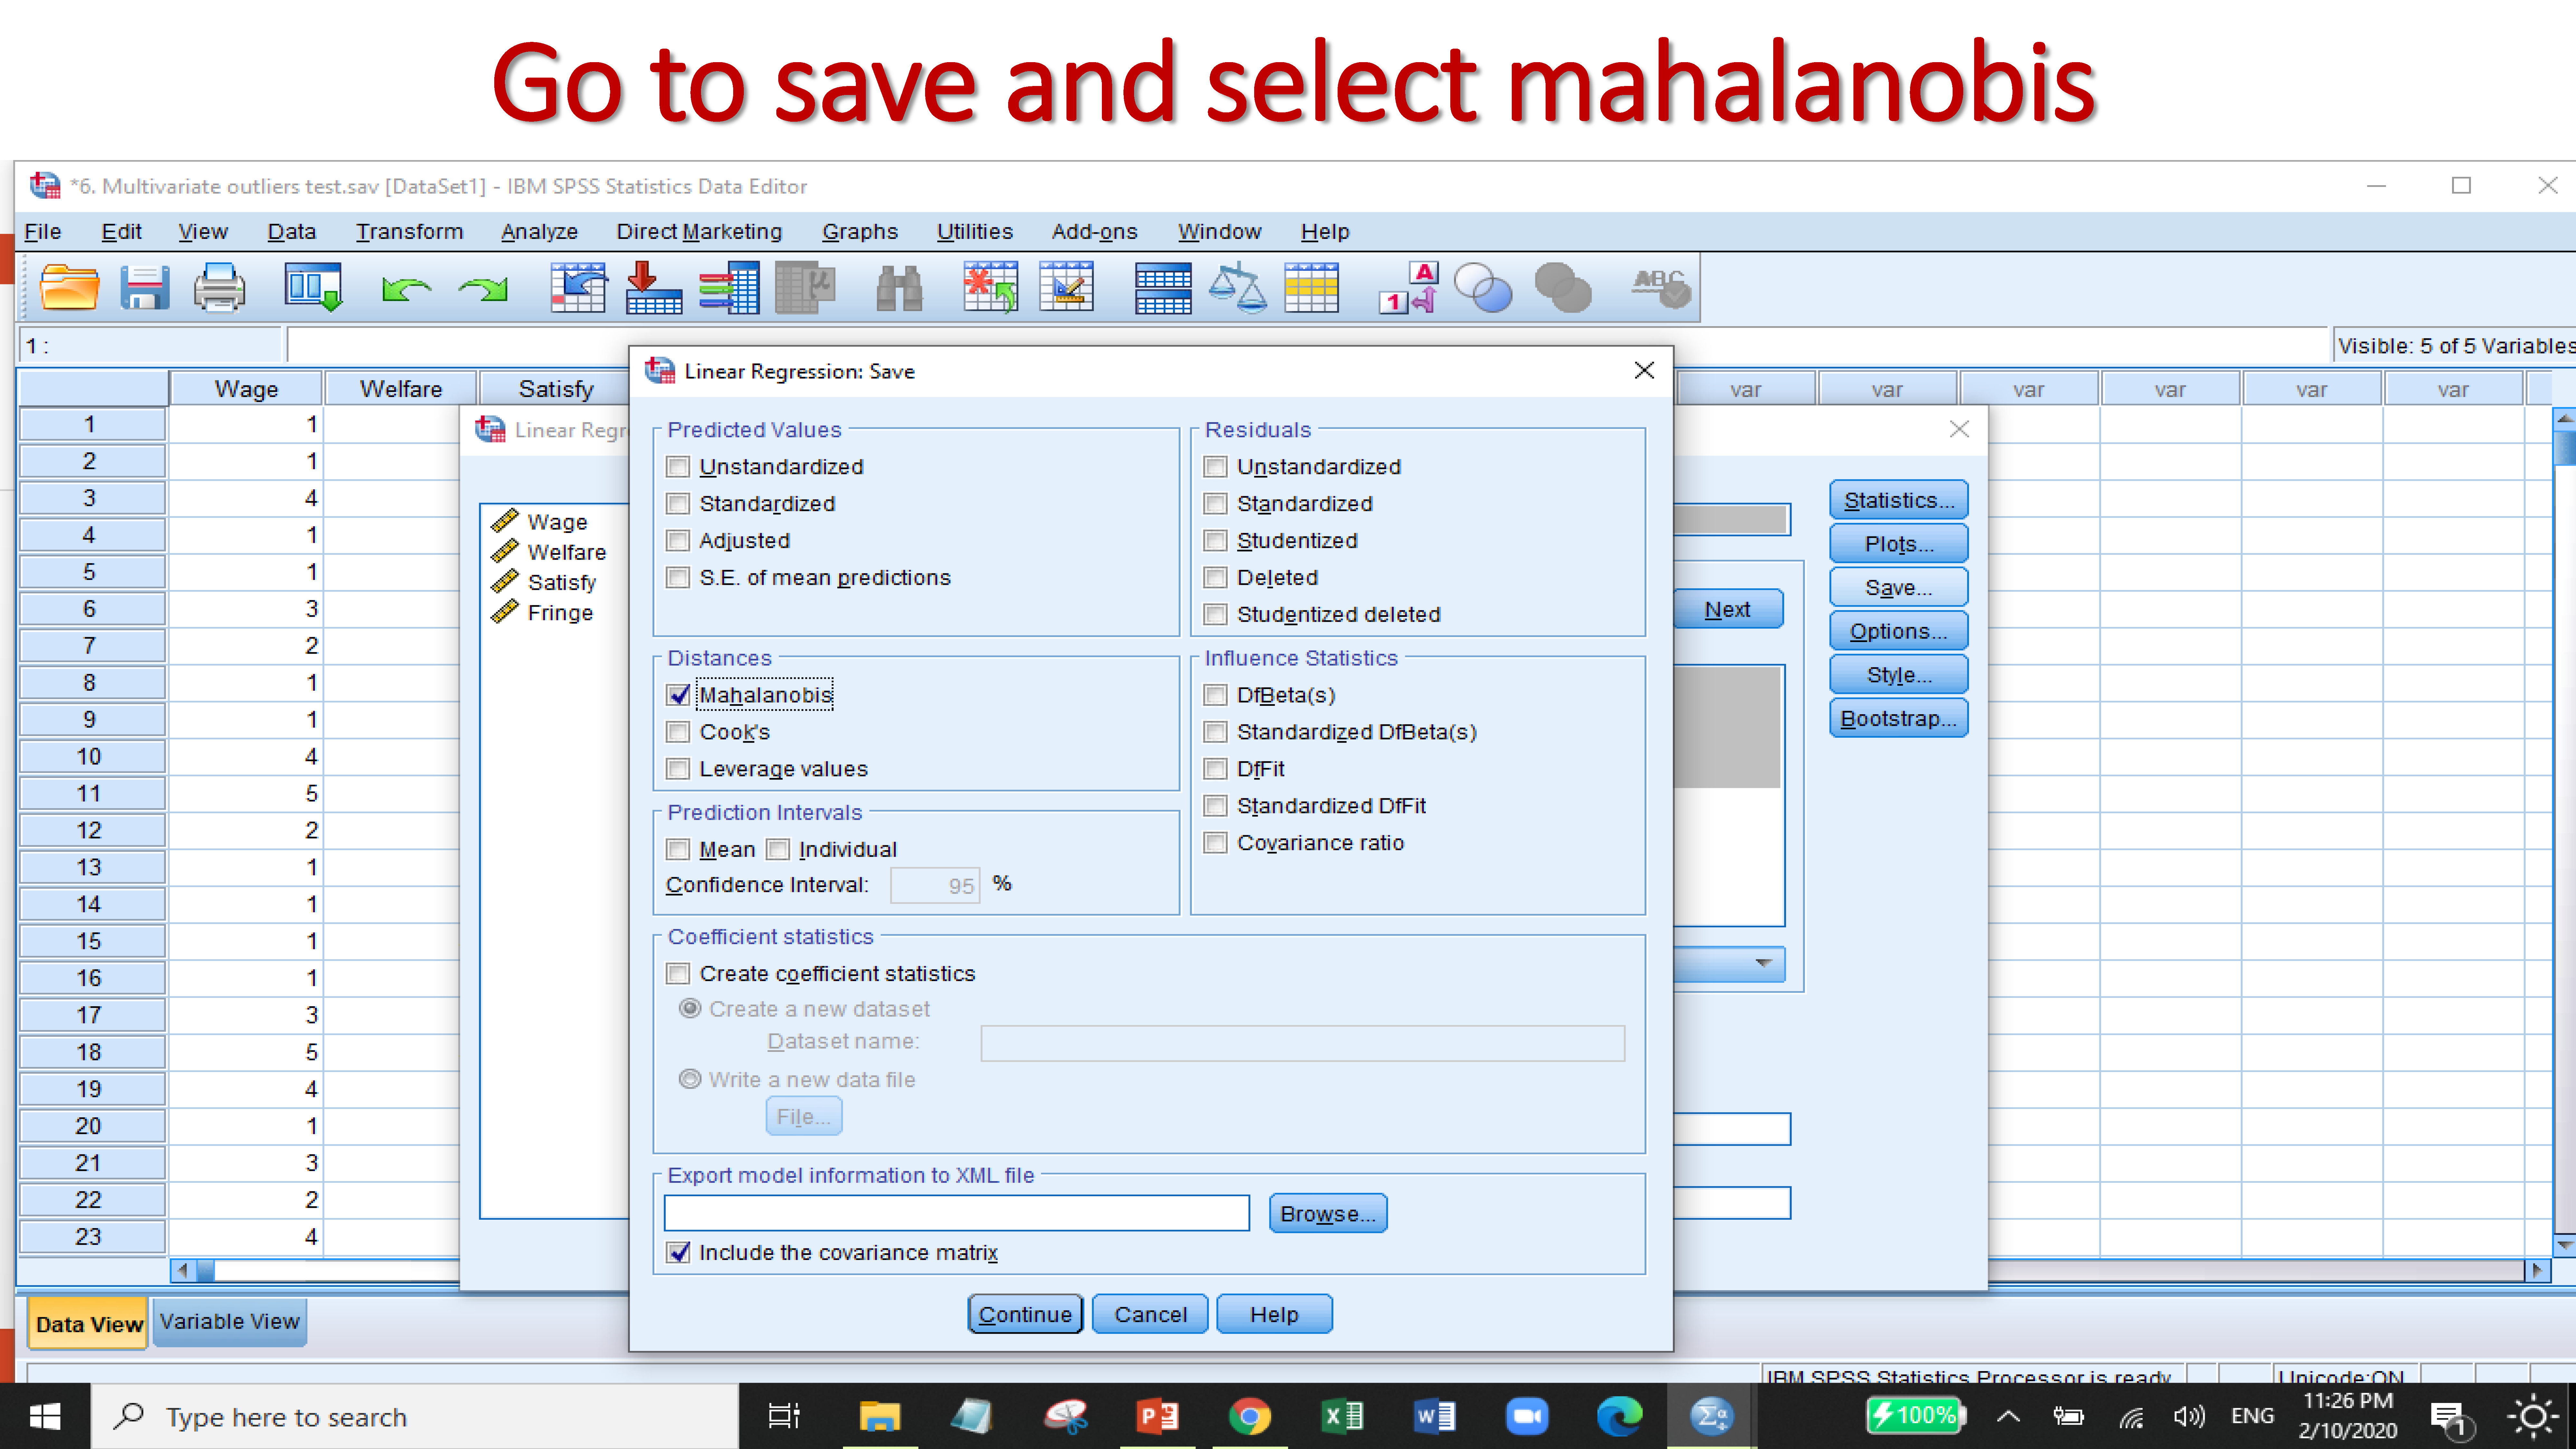
\includegraphics{images/slides/img_Page_051.png}

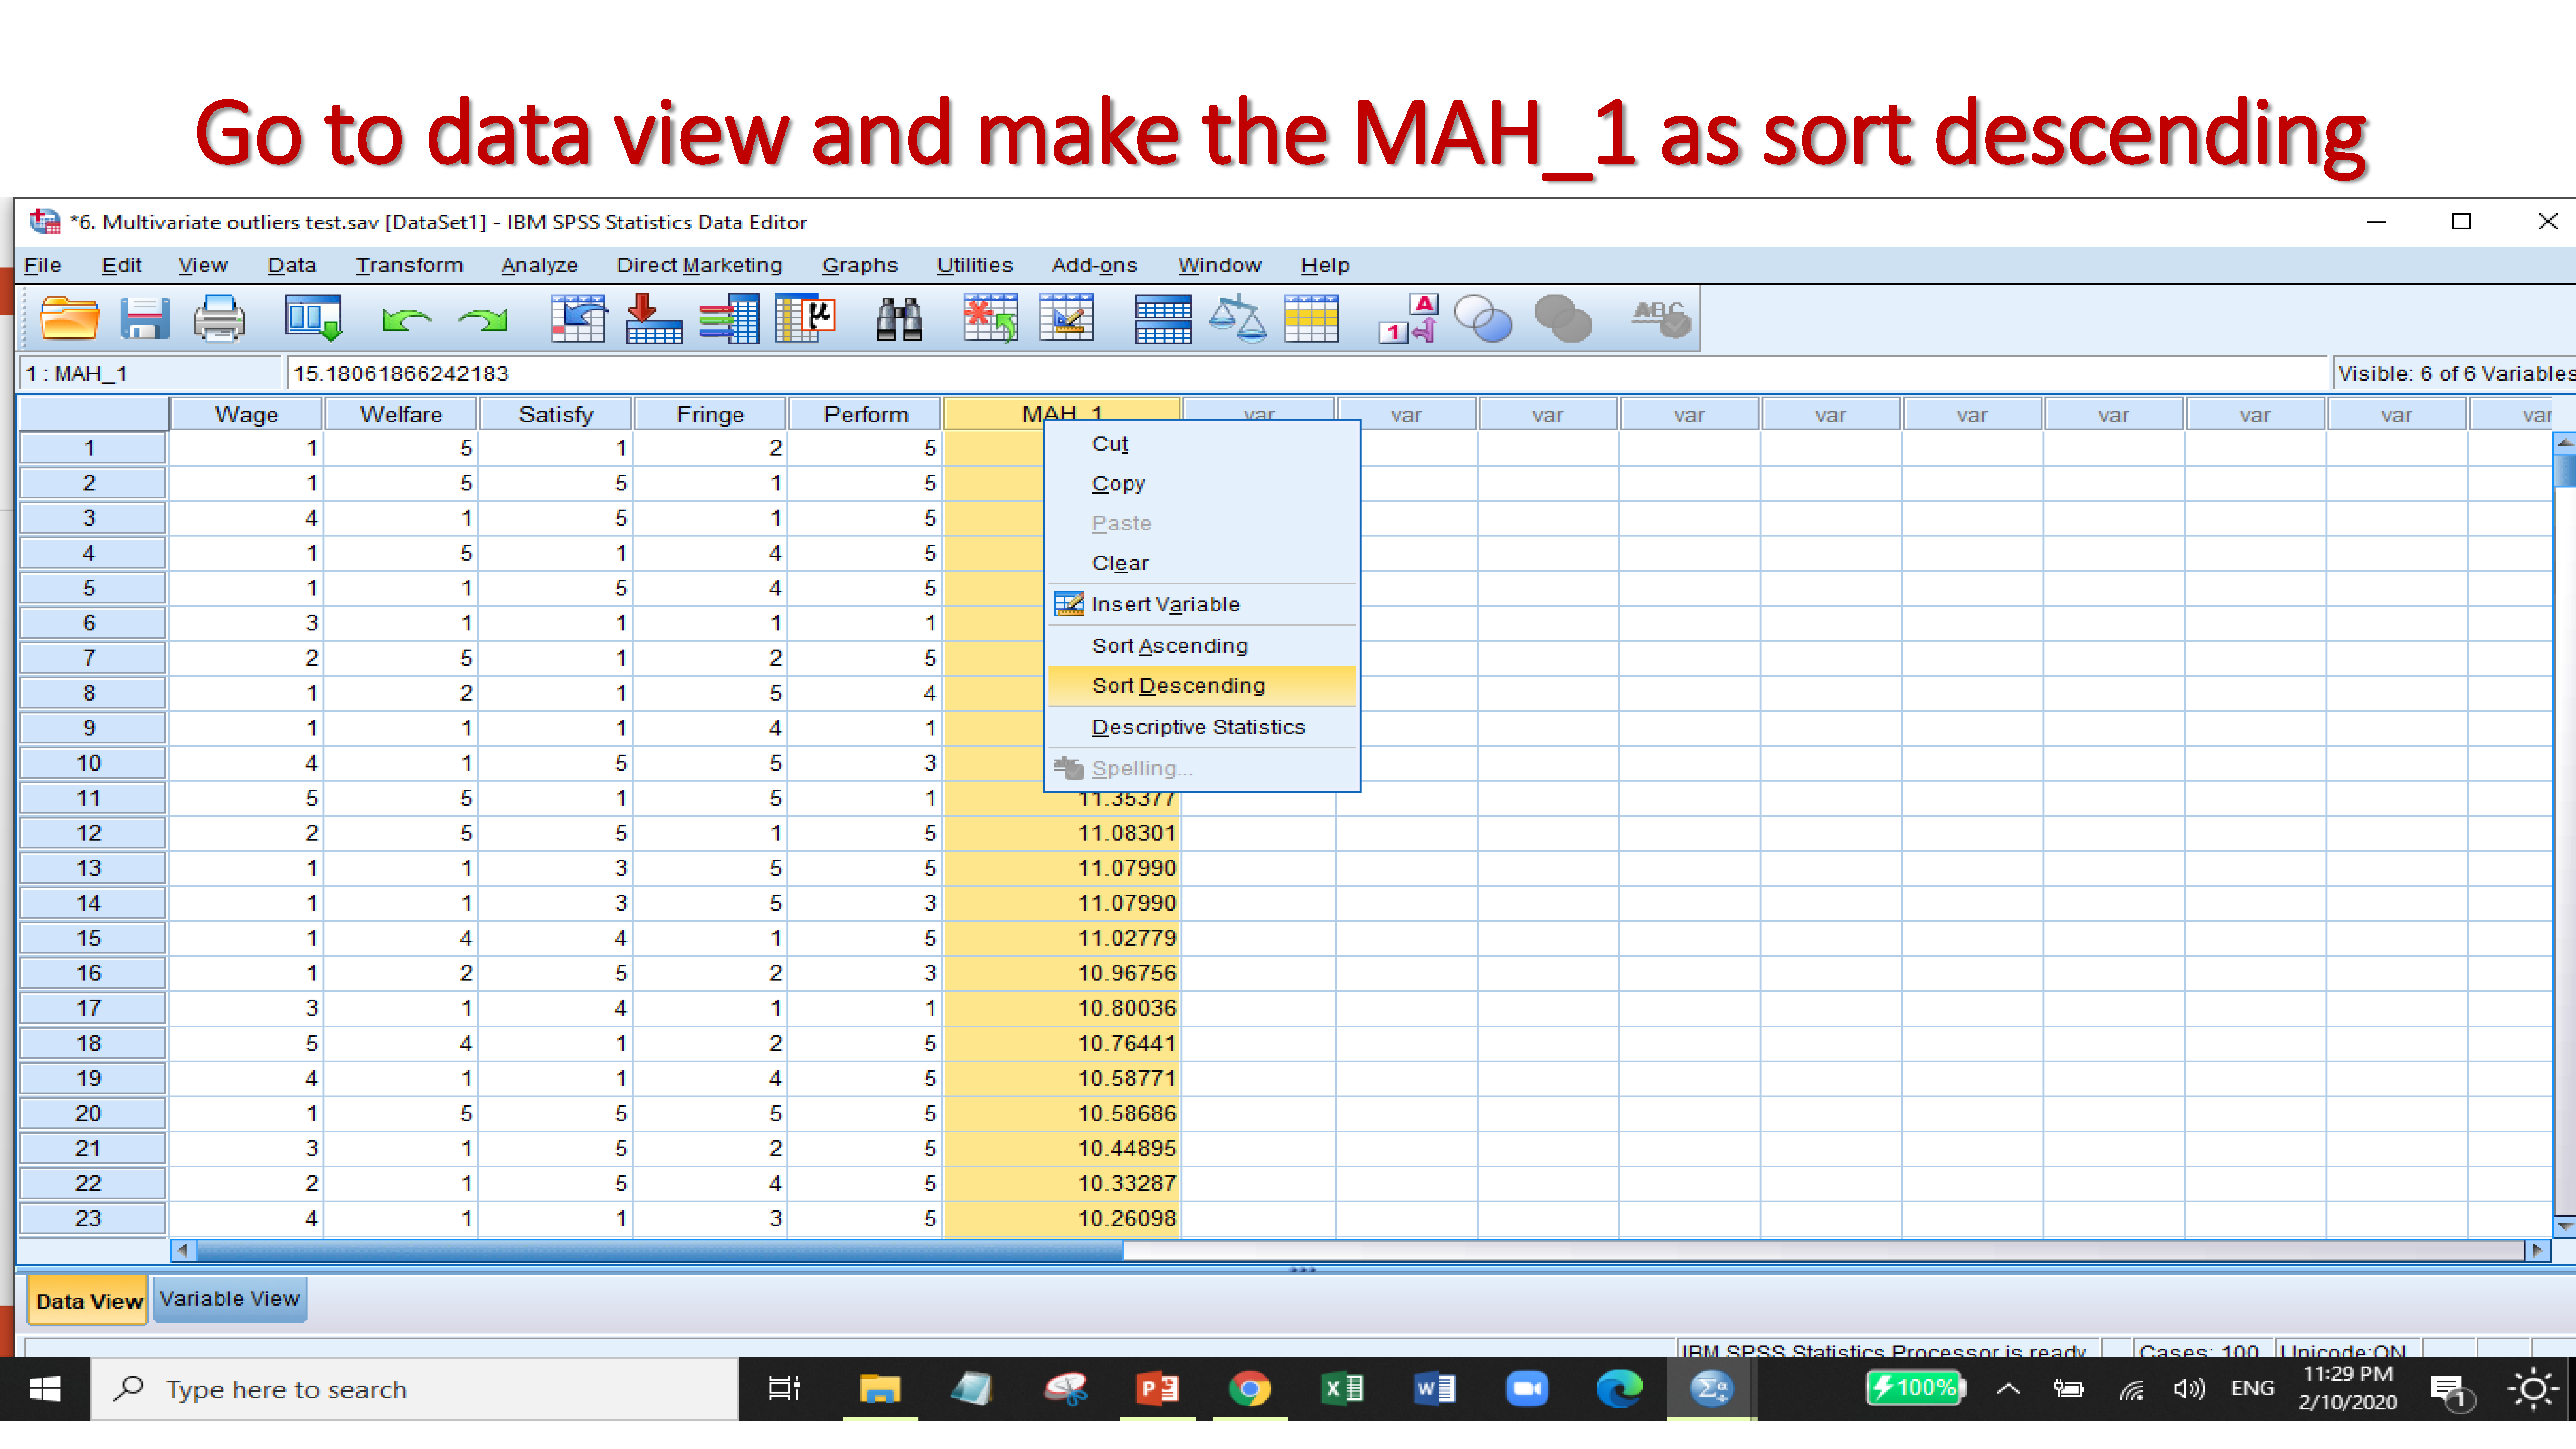
\includegraphics{images/slides/img_Page_052.png}

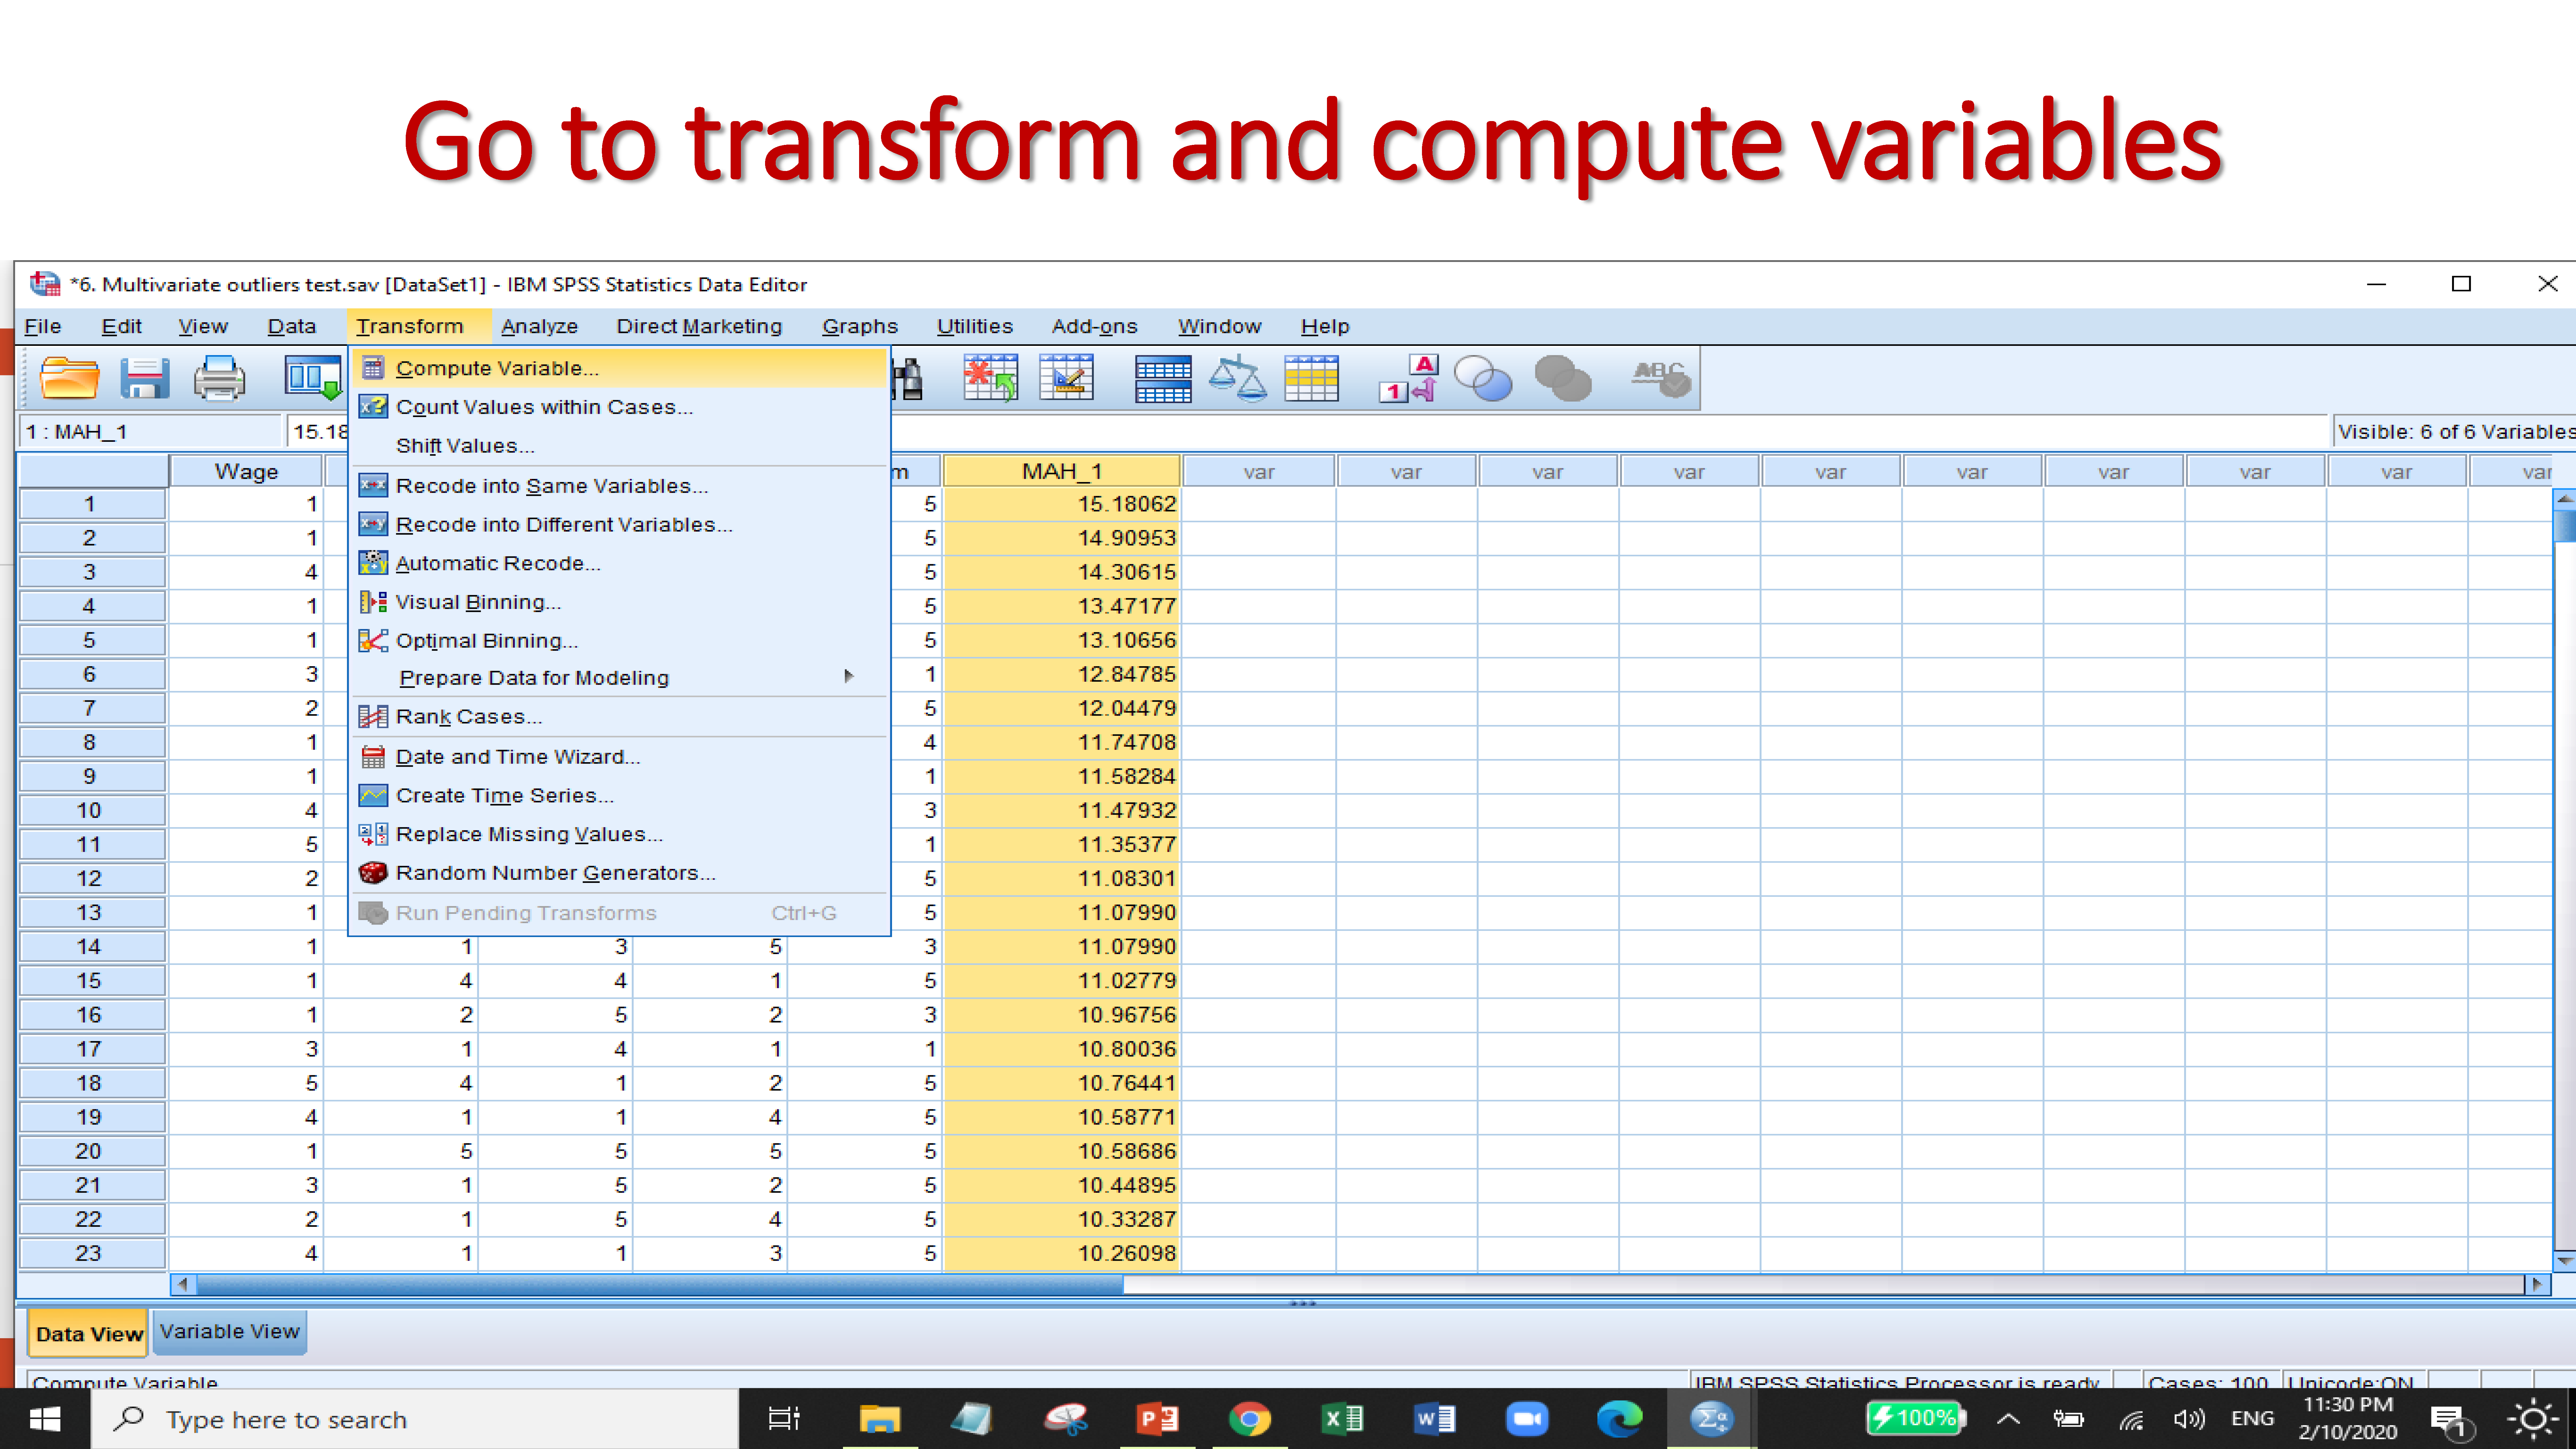
\includegraphics{images/slides/img_Page_053.png}

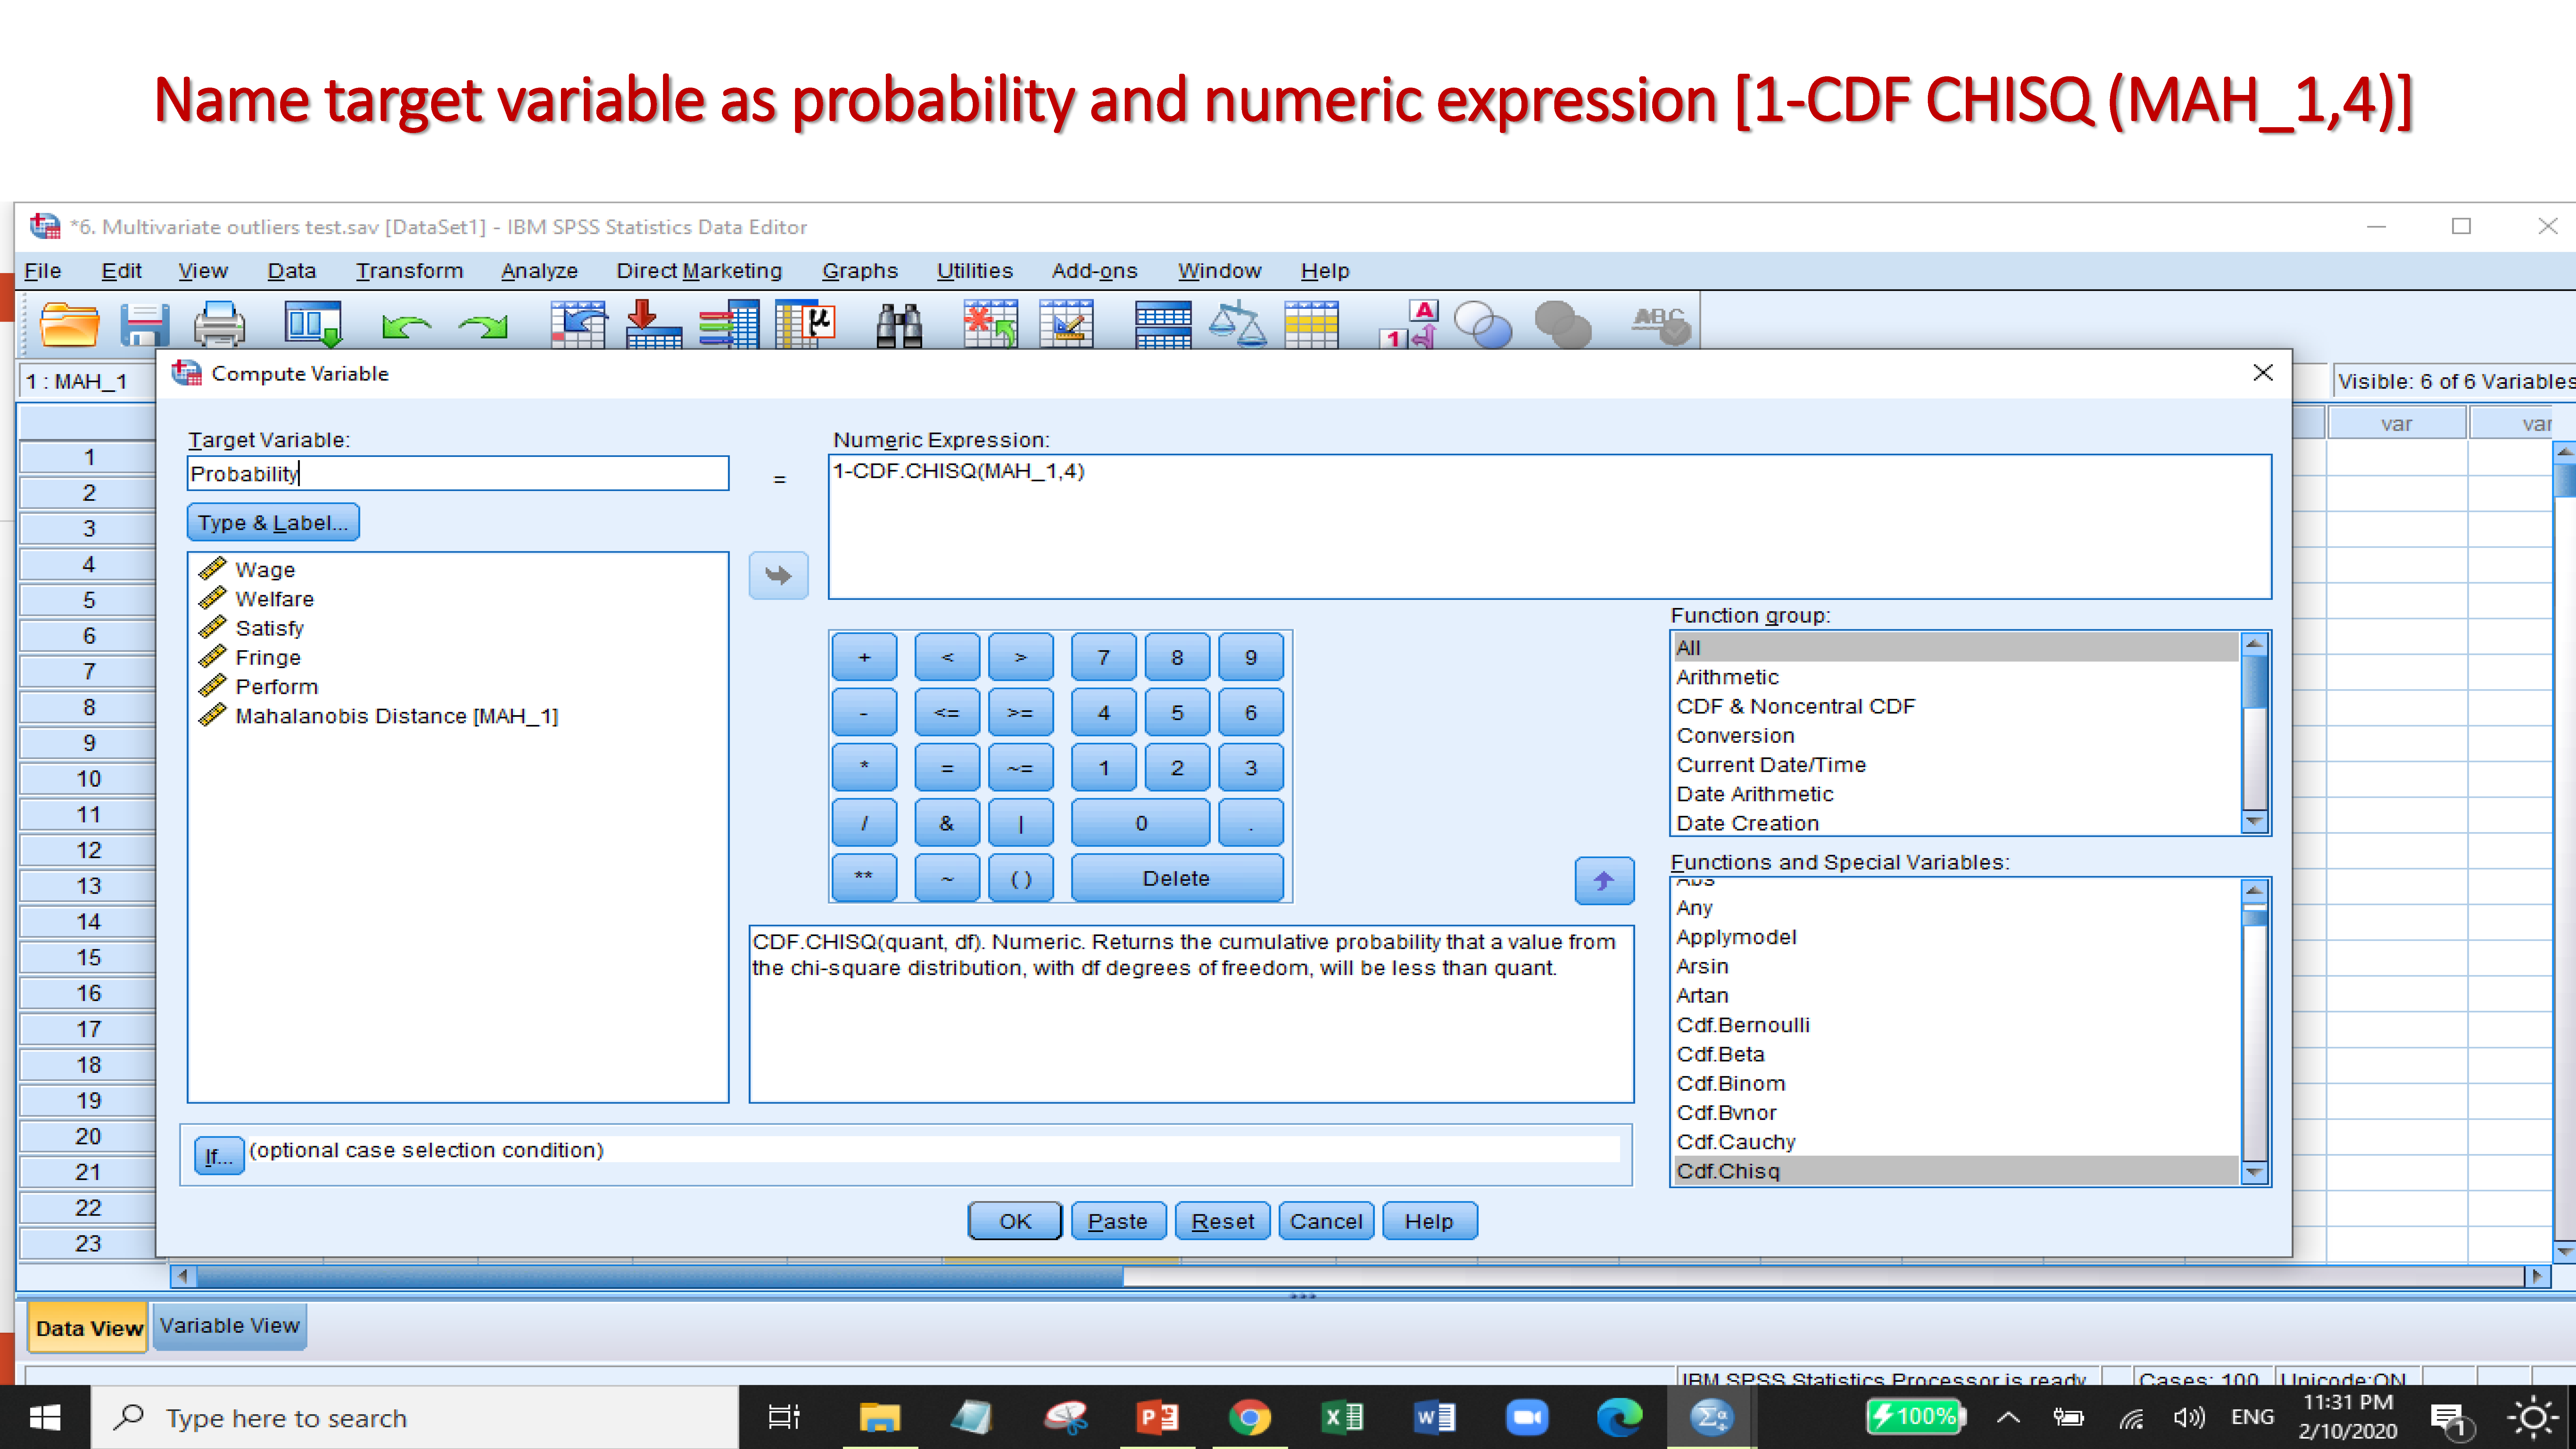
\includegraphics{images/slides/img_Page_054.png}

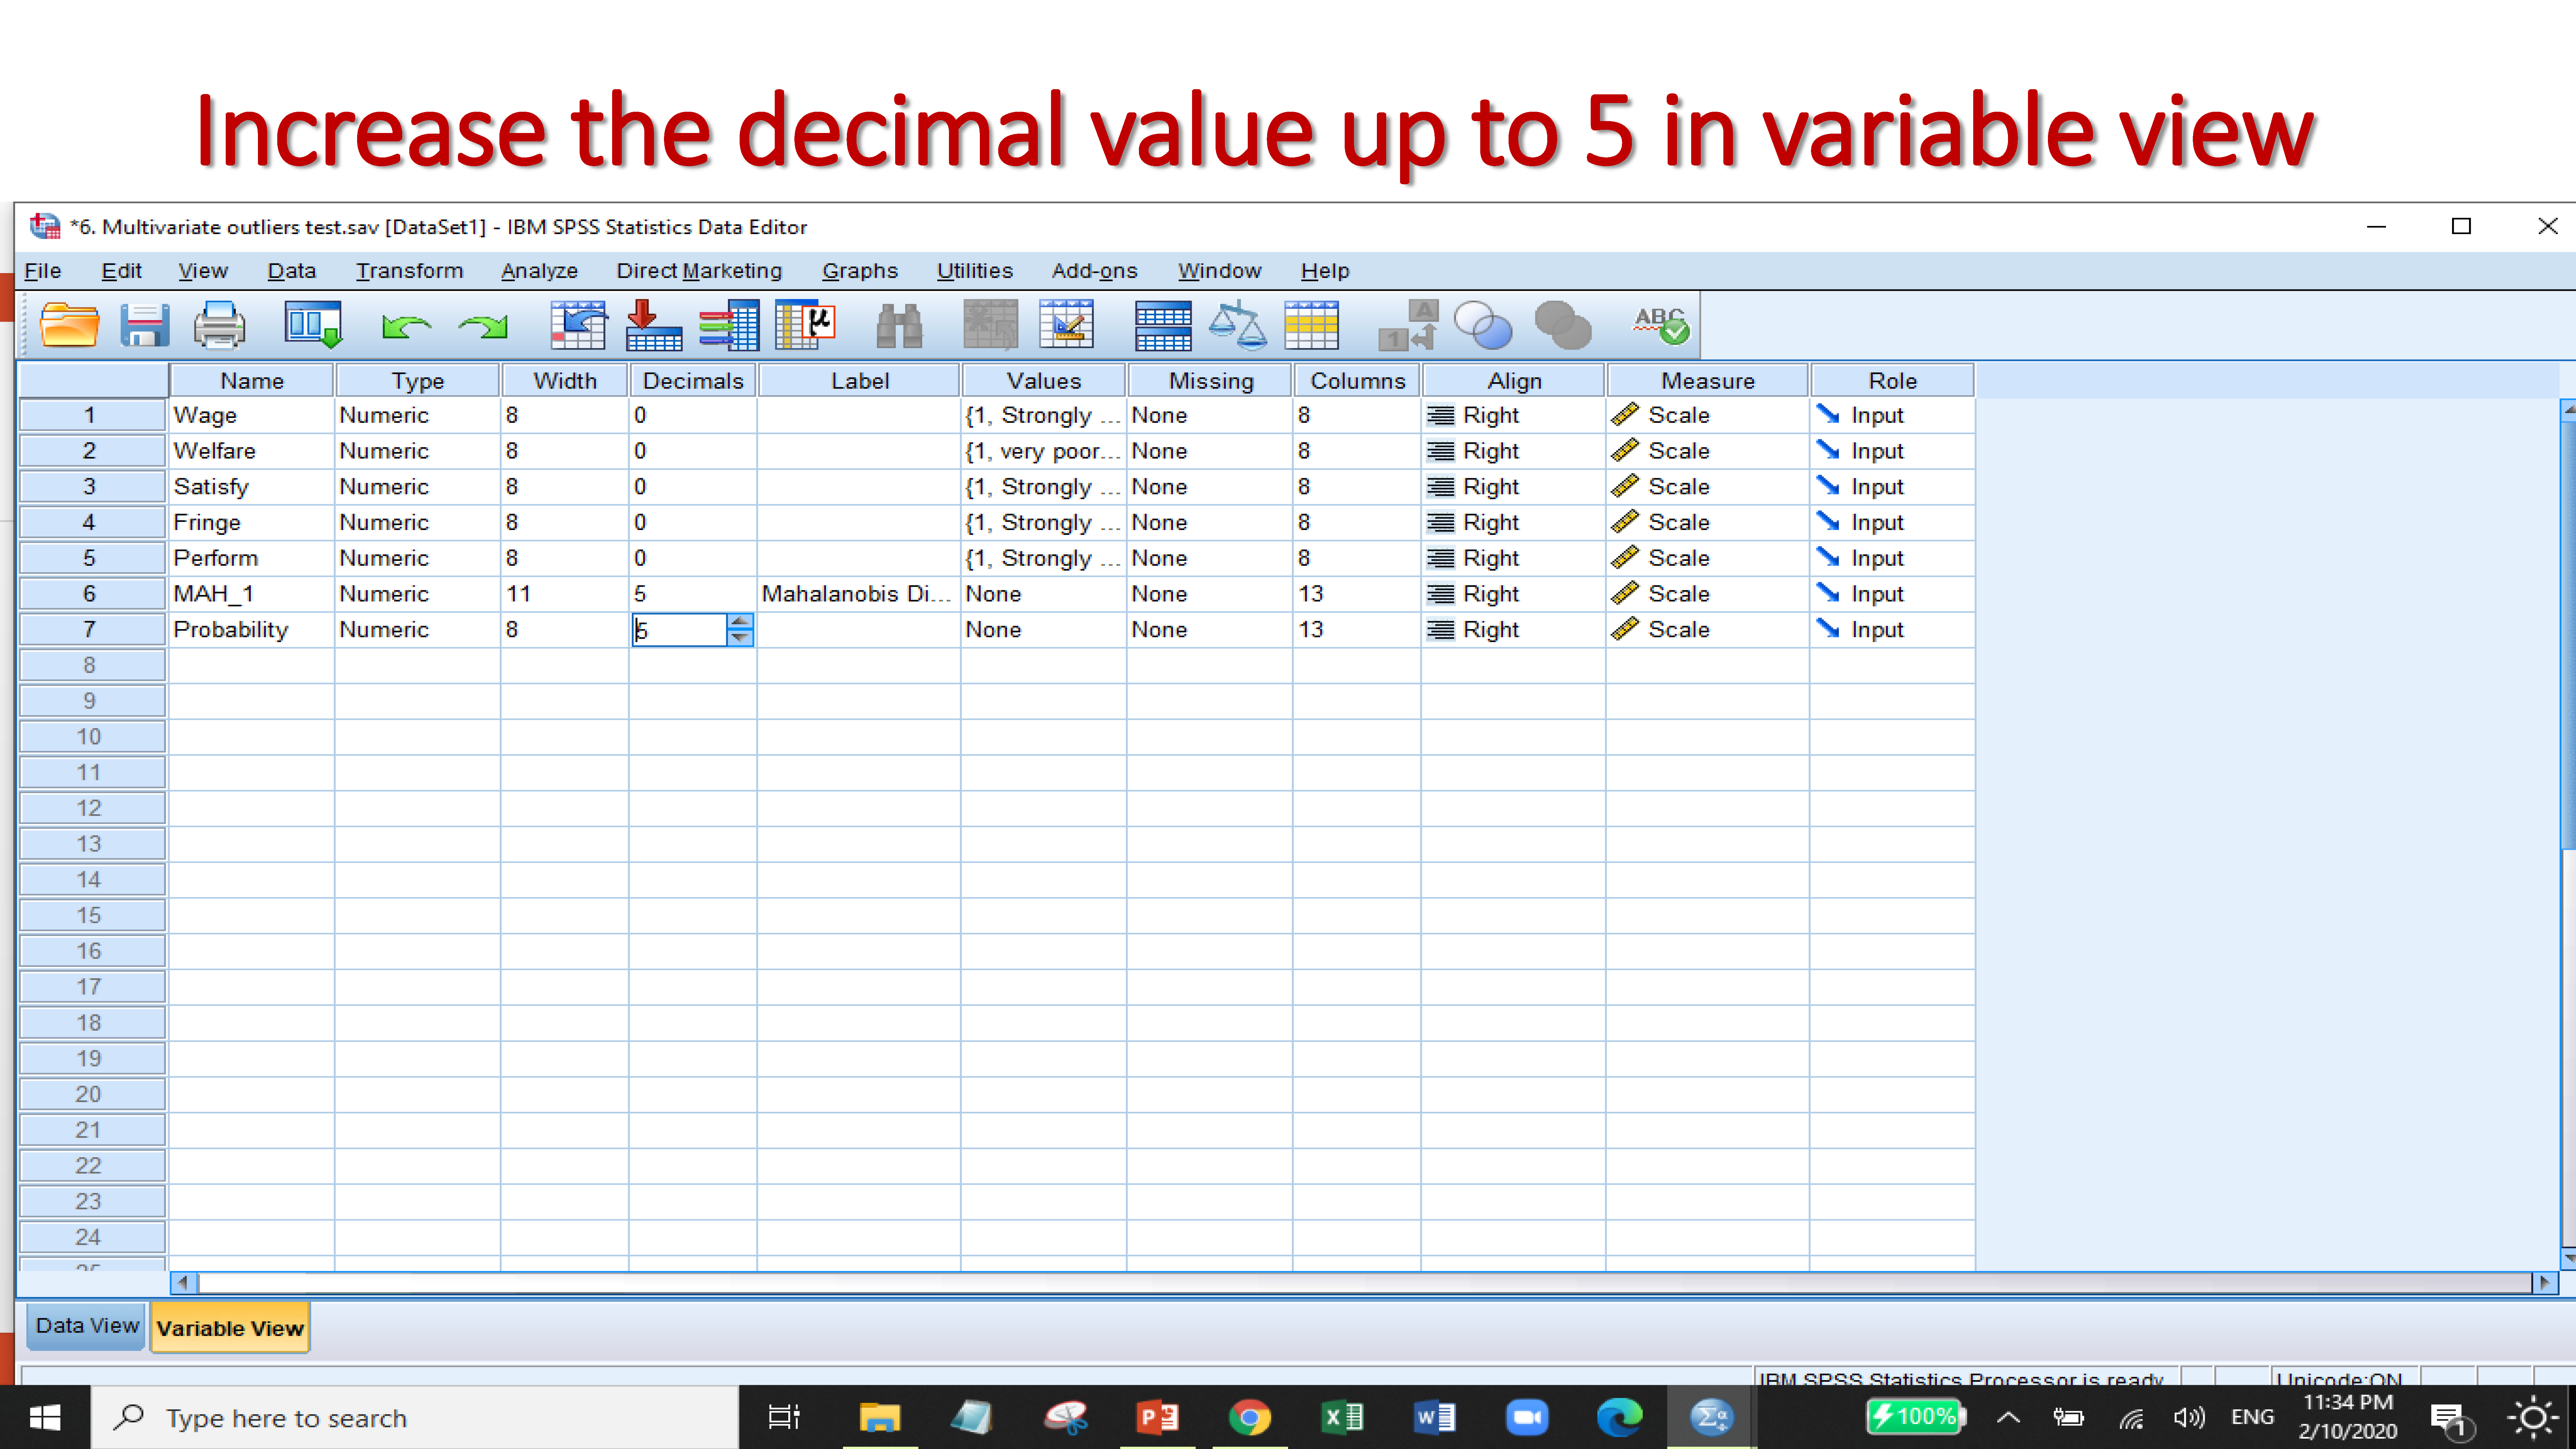
\includegraphics{images/slides/img_Page_055.png}

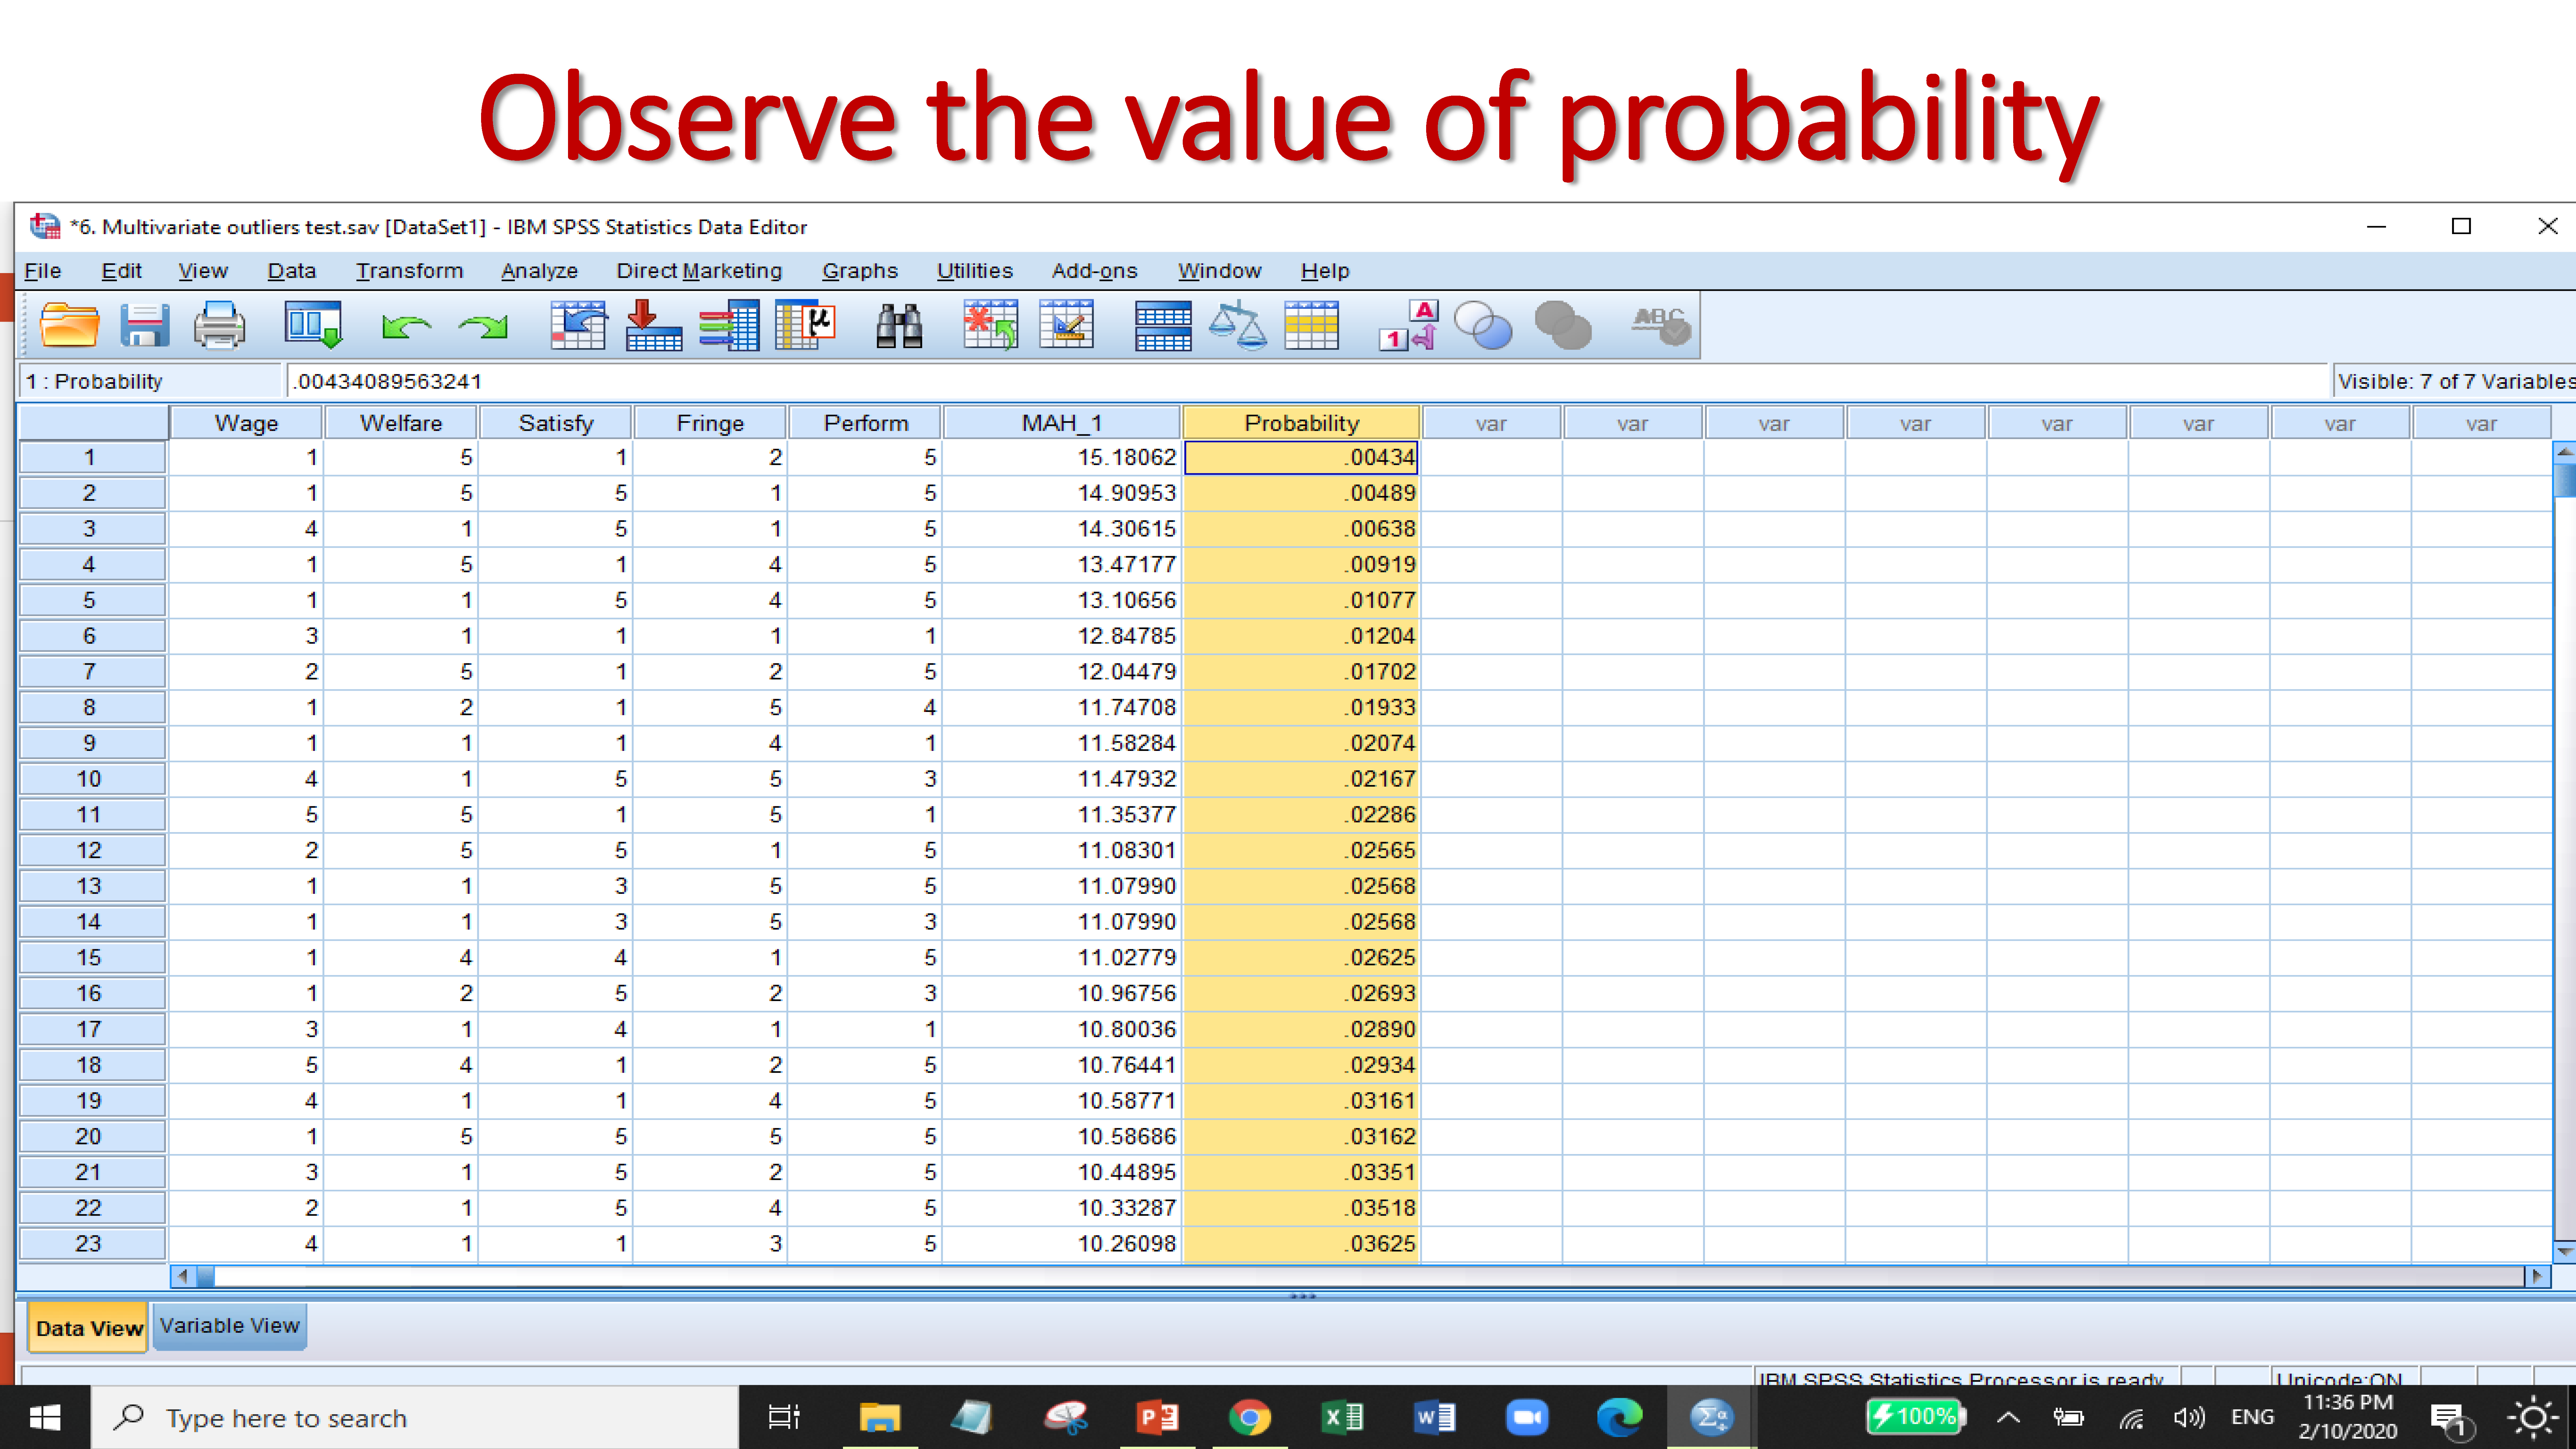
\includegraphics{images/slides/img_Page_056.png}

\begin{tcolorbox}[enhanced jigsaw, rightrule=.15mm, arc=.35mm, colframe=quarto-callout-note-color-frame, coltitle=black, left=2mm, colbacktitle=quarto-callout-note-color!10!white, bottomtitle=1mm, titlerule=0mm, colback=white, breakable, opacitybacktitle=0.6, opacityback=0, toprule=.15mm, toptitle=1mm, title=\textcolor{quarto-callout-note-color}{\faInfo}\hspace{0.5em}{Decision Criteria}, bottomrule=.15mm, leftrule=.75mm]

If the value of probability less than 0.001 then the observations will
count as multivariate outliers.

\end{tcolorbox}

\bookmarksetup{startatroot}

\chapter{Test of Data Reliability (Cronbach's
alpha)}\label{test-of-data-reliability-cronbachs-alpha}

\textbf{Cronbach's alpha} is a measure of internal consistency, that is,
how closely related a set of items are as a group. It is considered to
be a measure of scale reliability\\

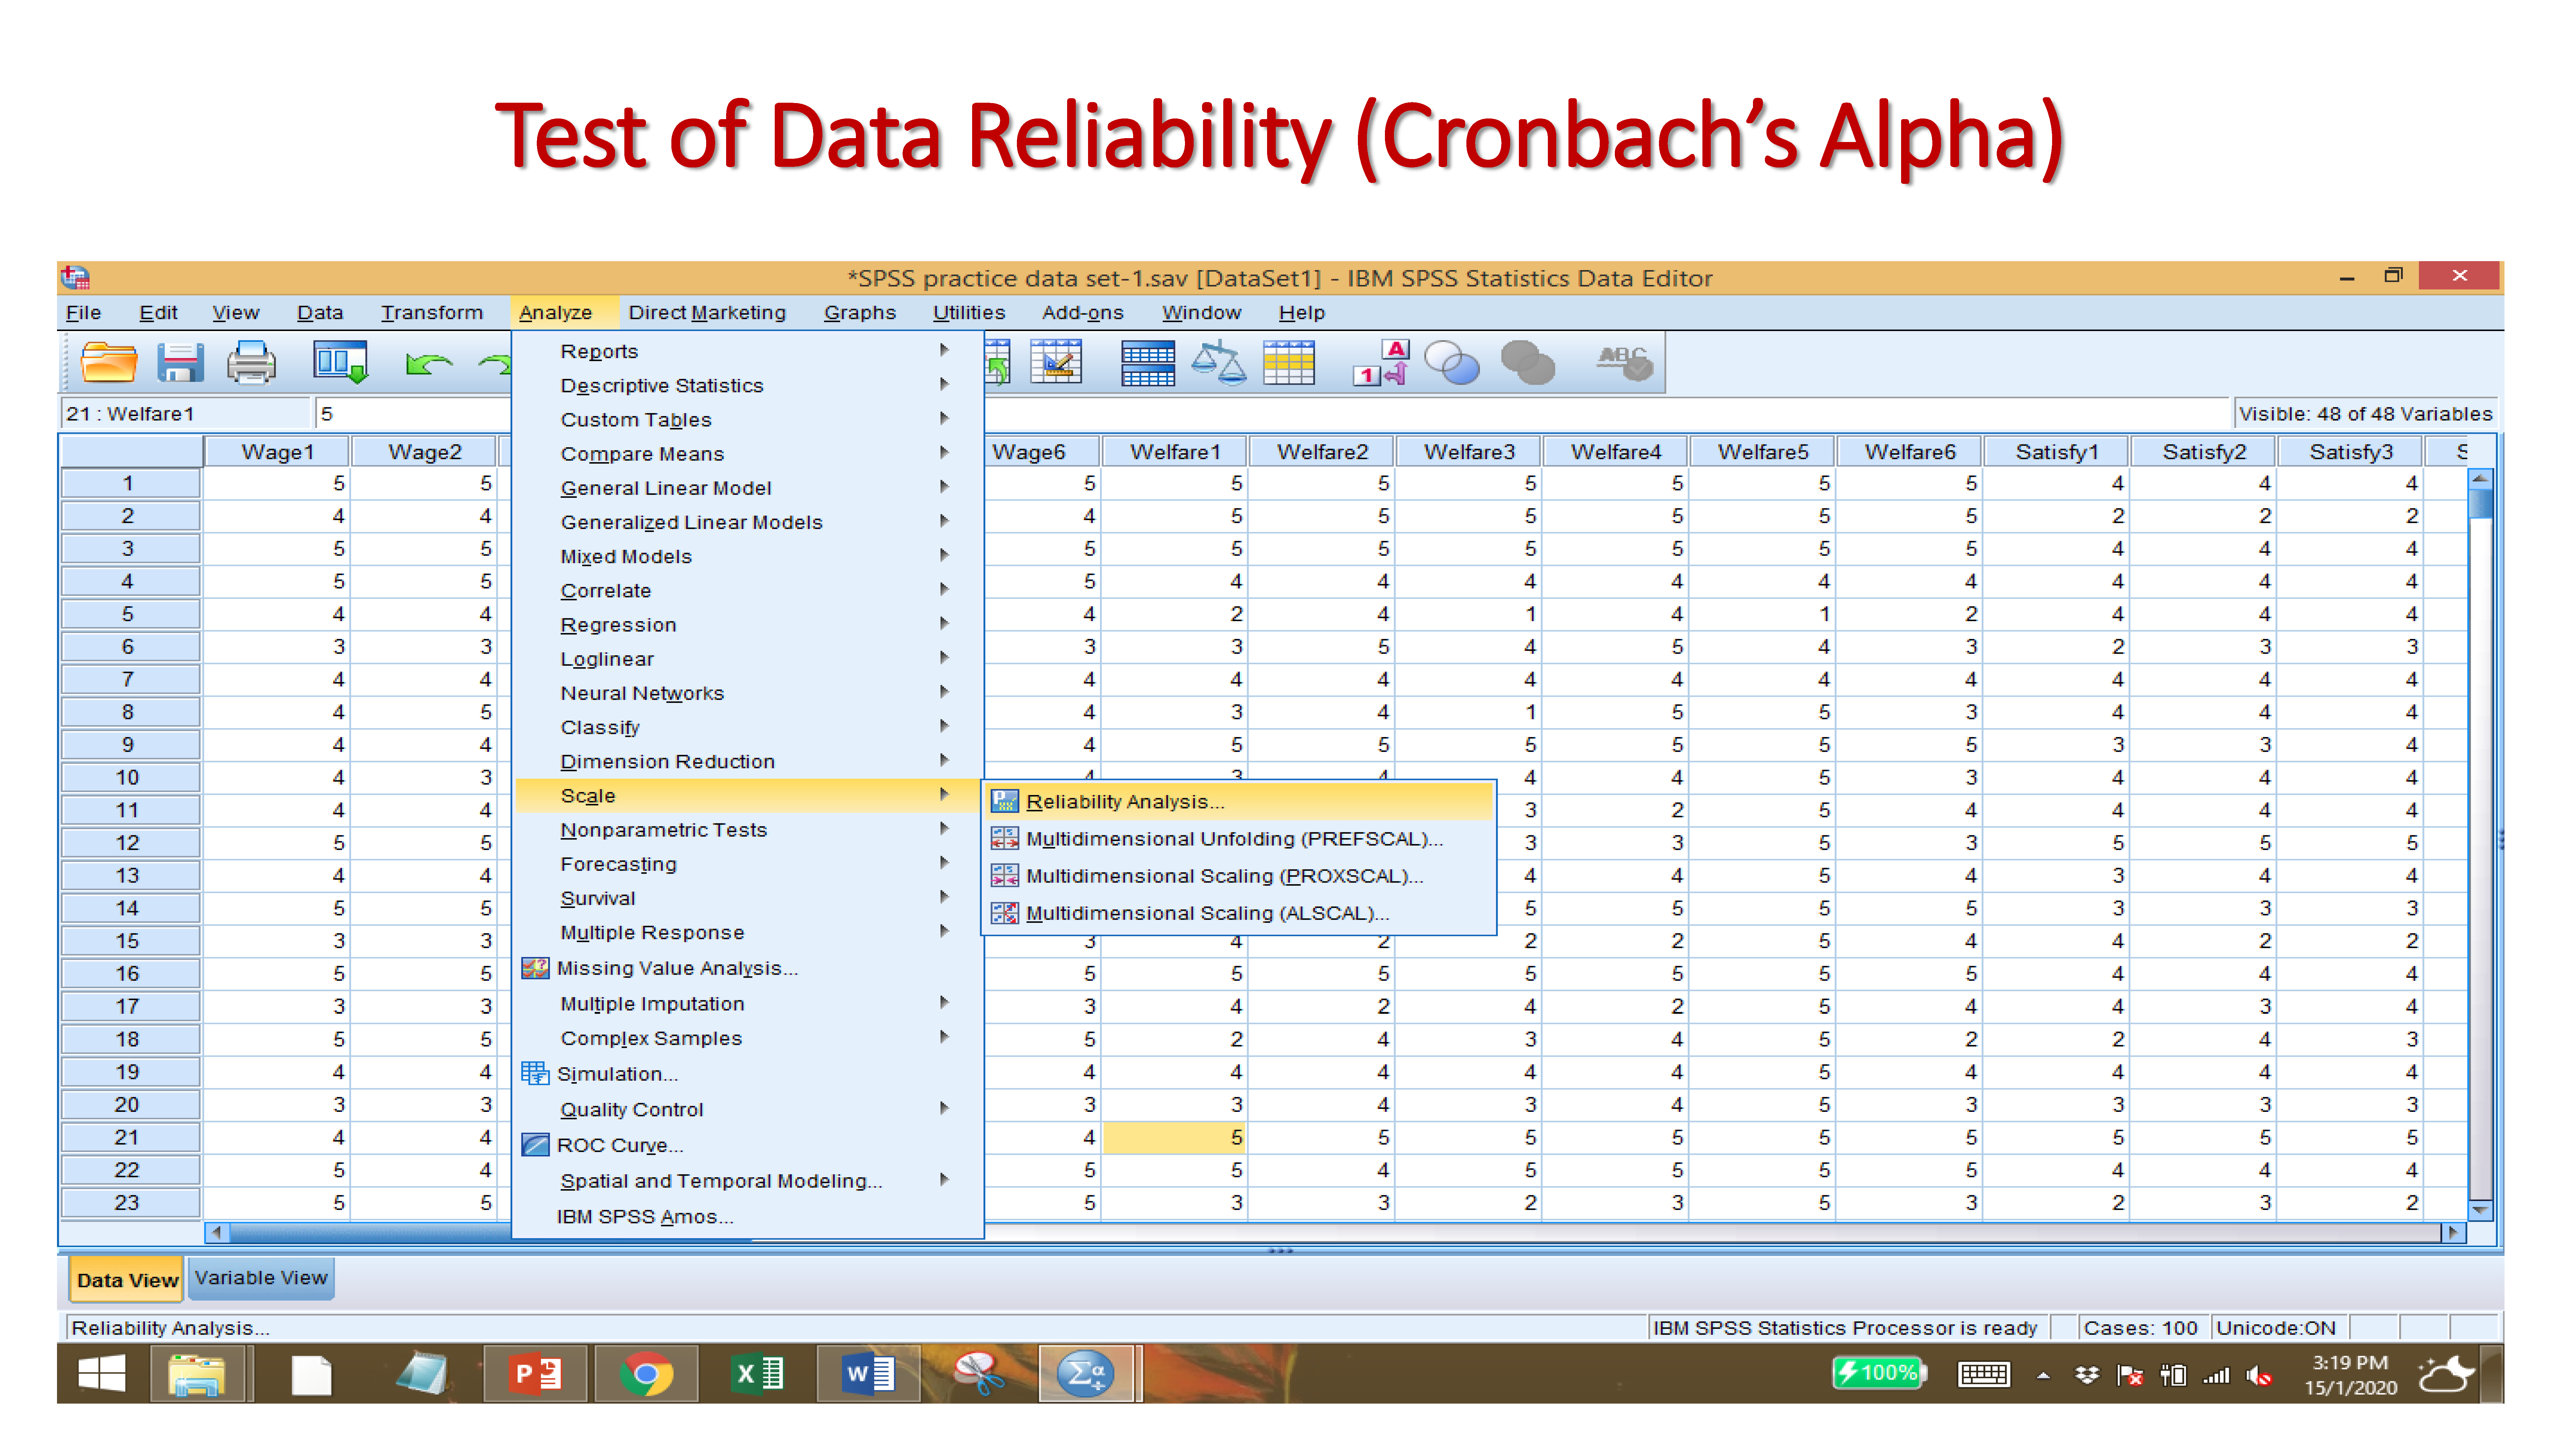
\includegraphics{images/slides/img_Page_059.png}

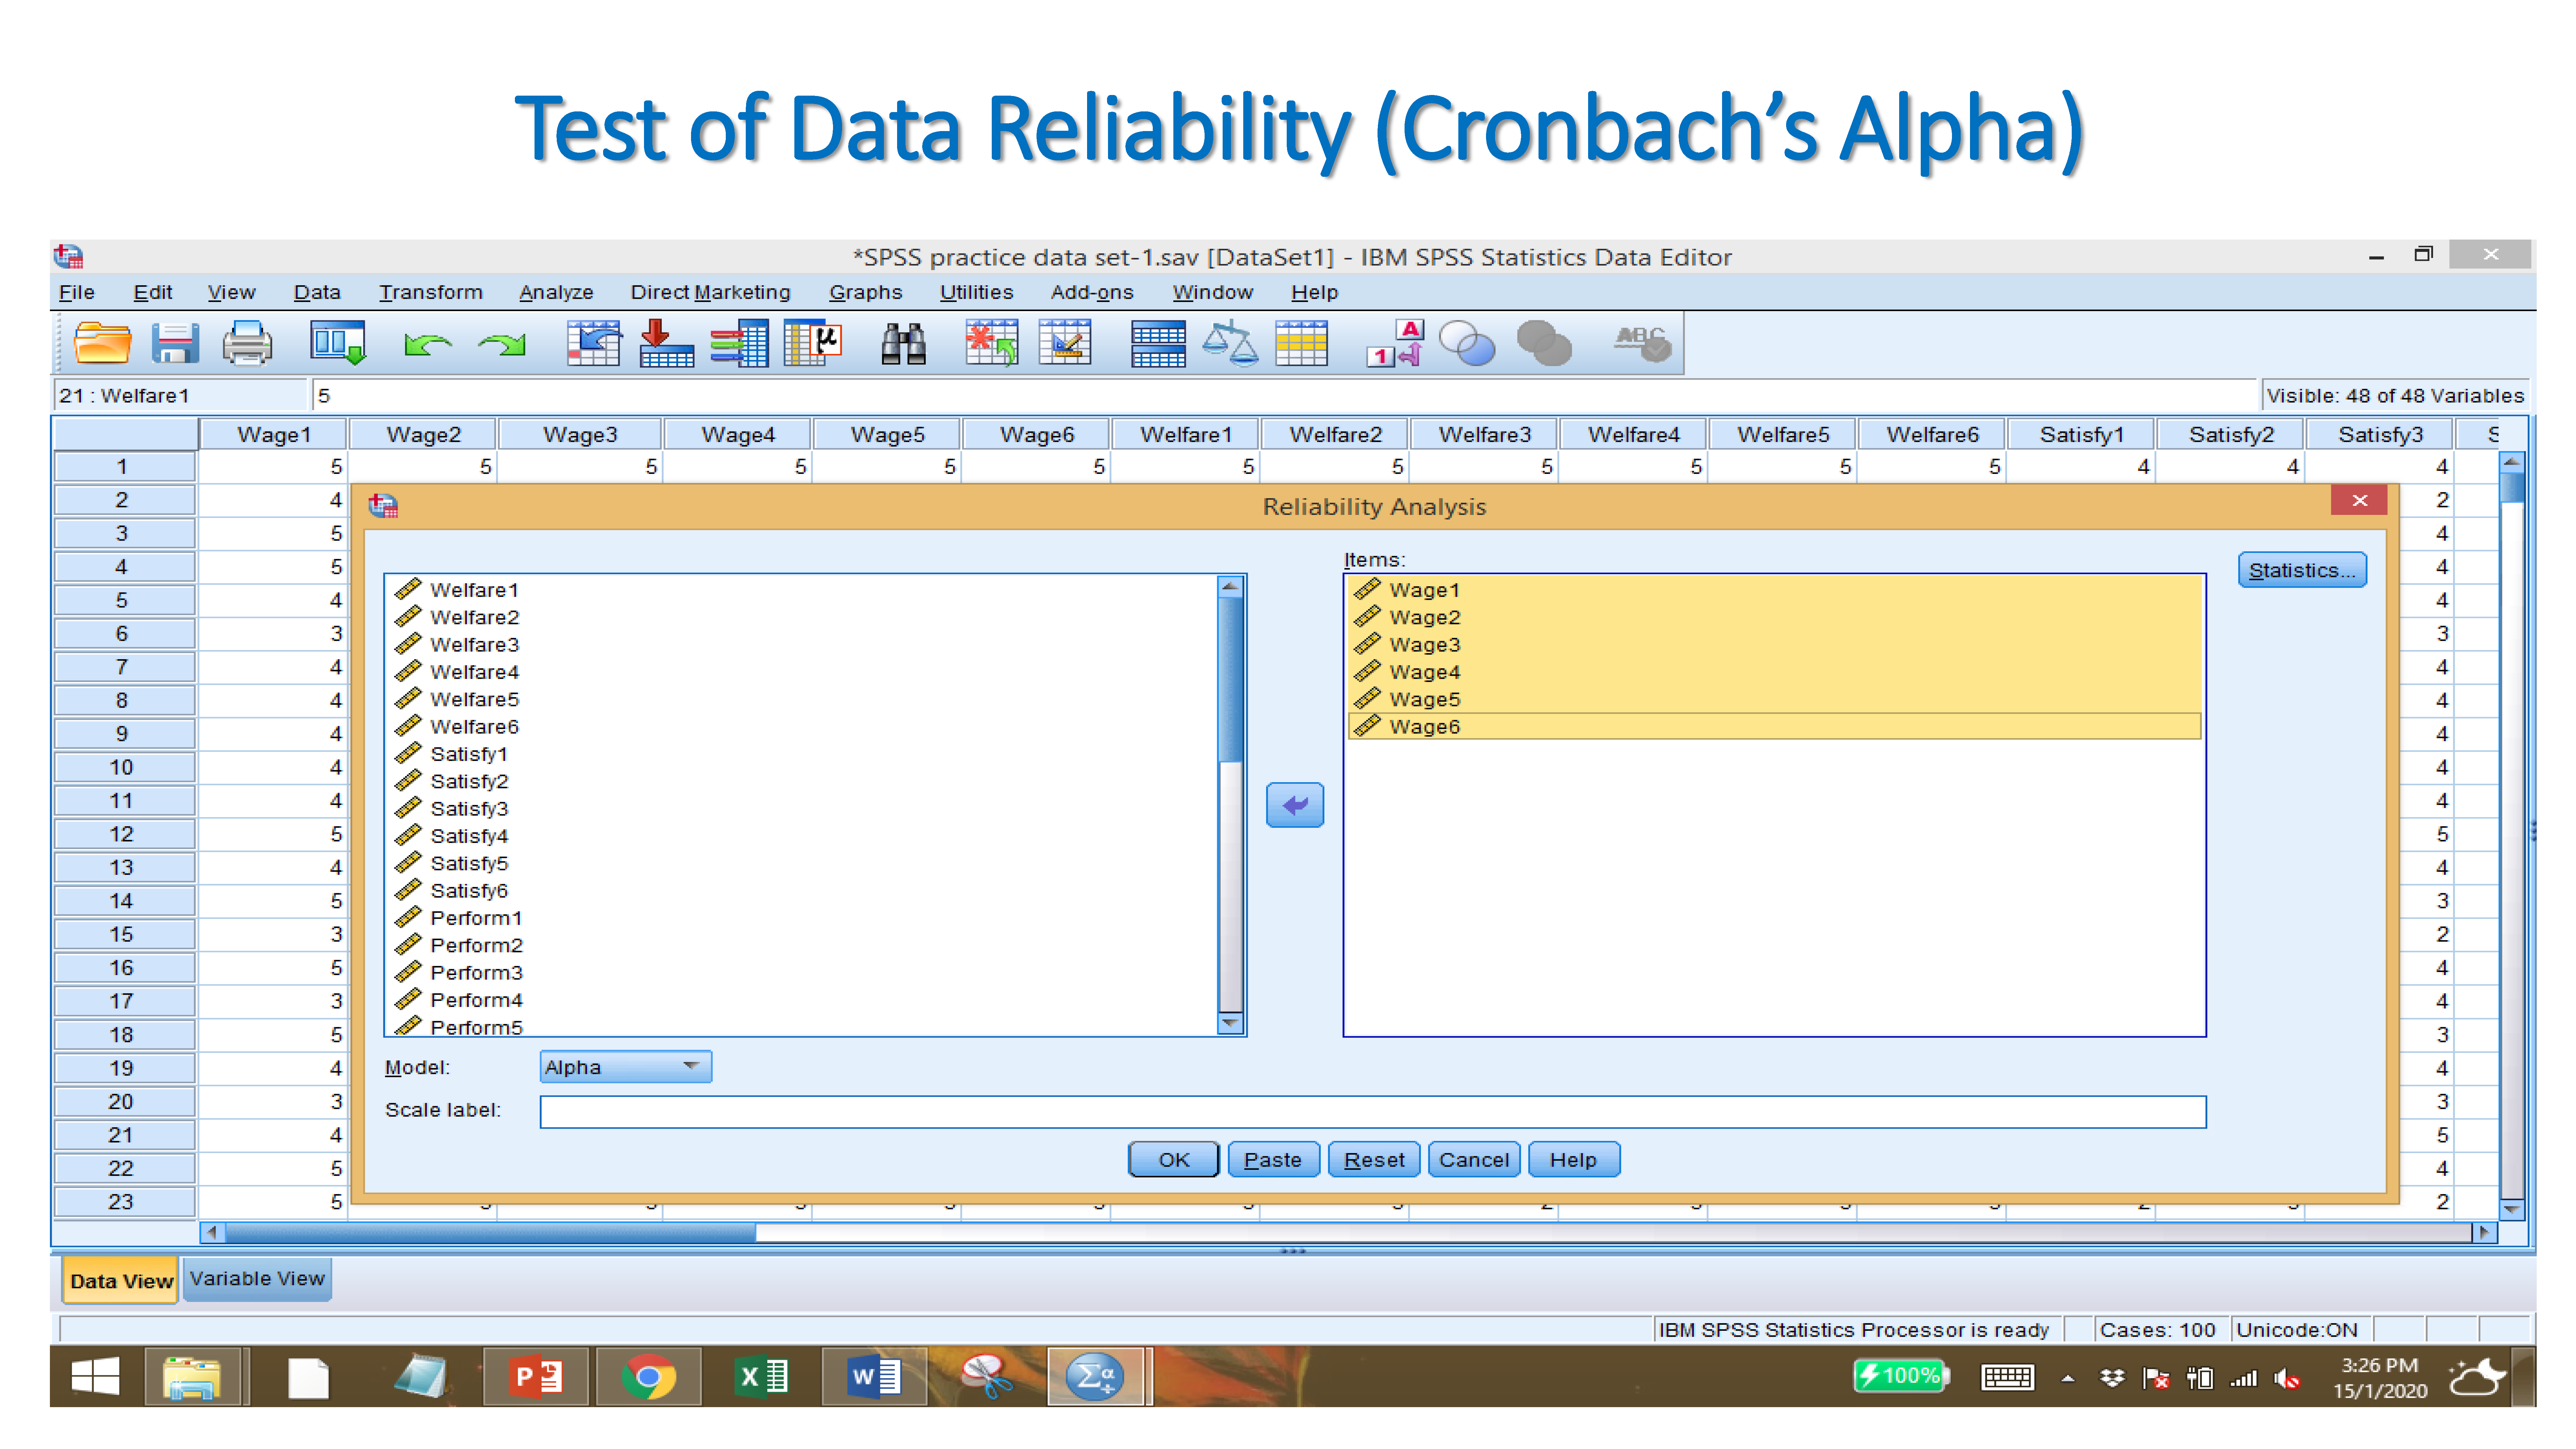
\includegraphics{images/slides/img_Page_060.png}

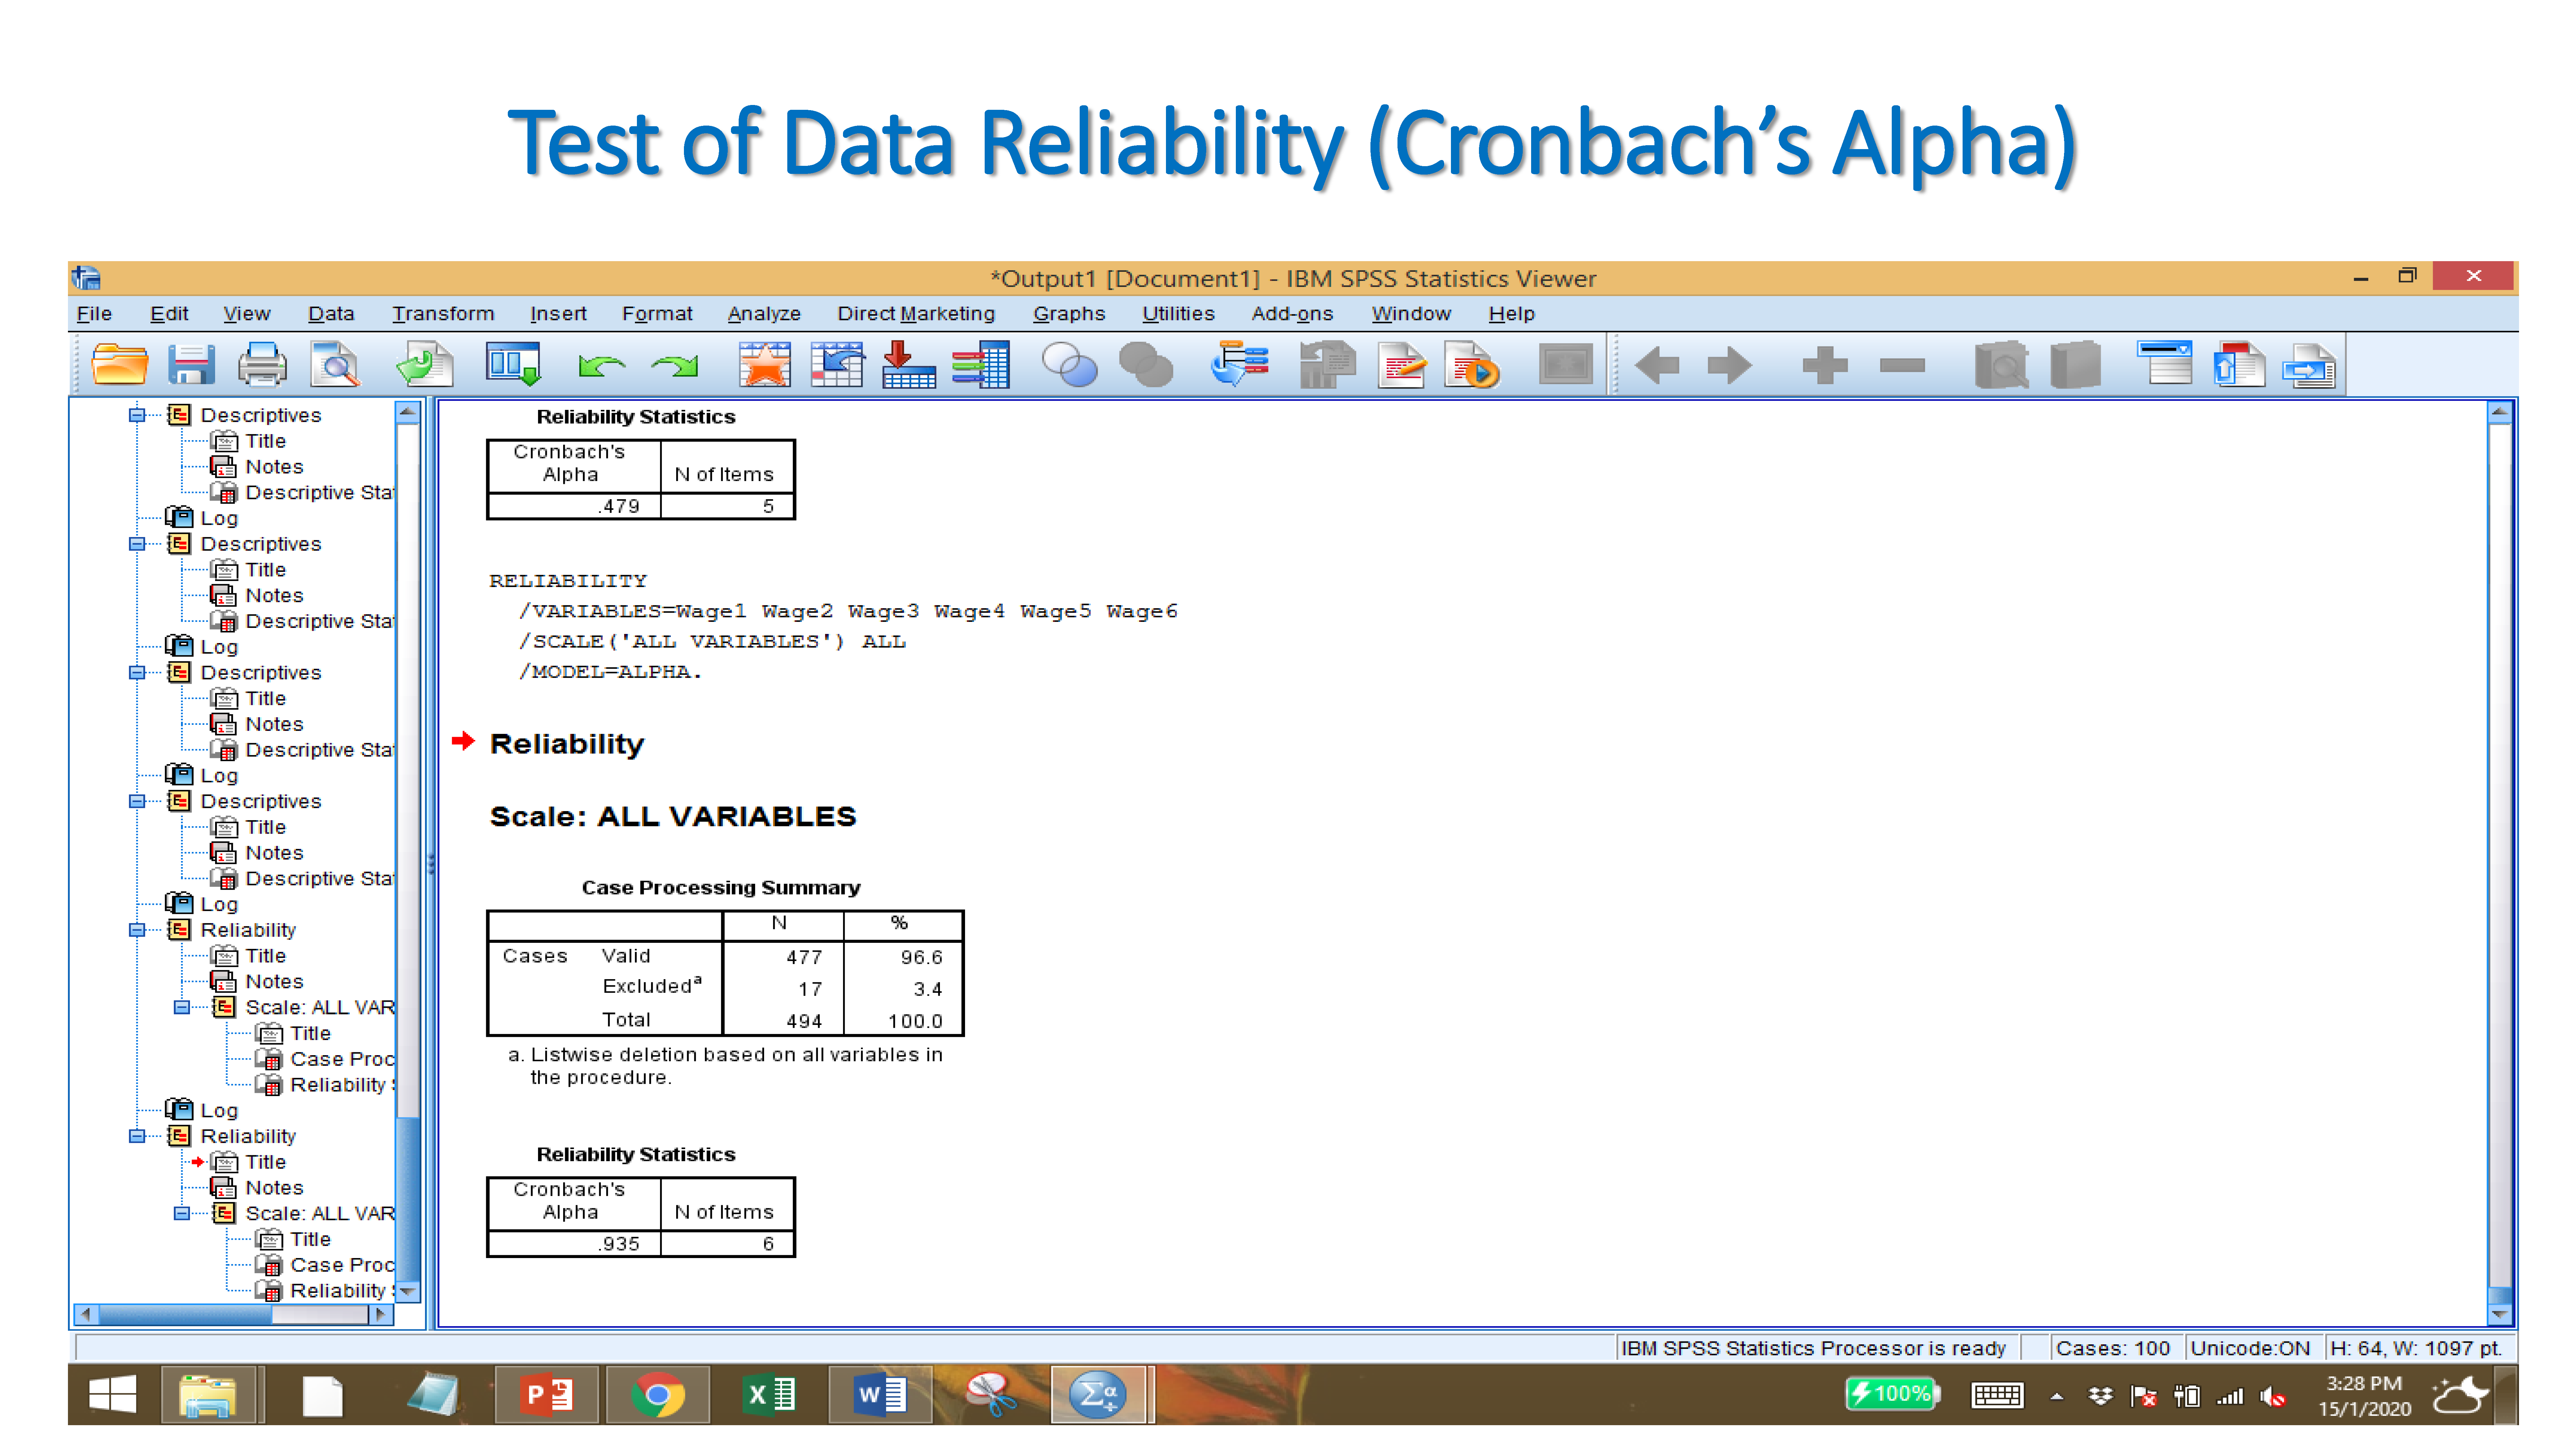
\includegraphics{images/slides/img_Page_061.png}

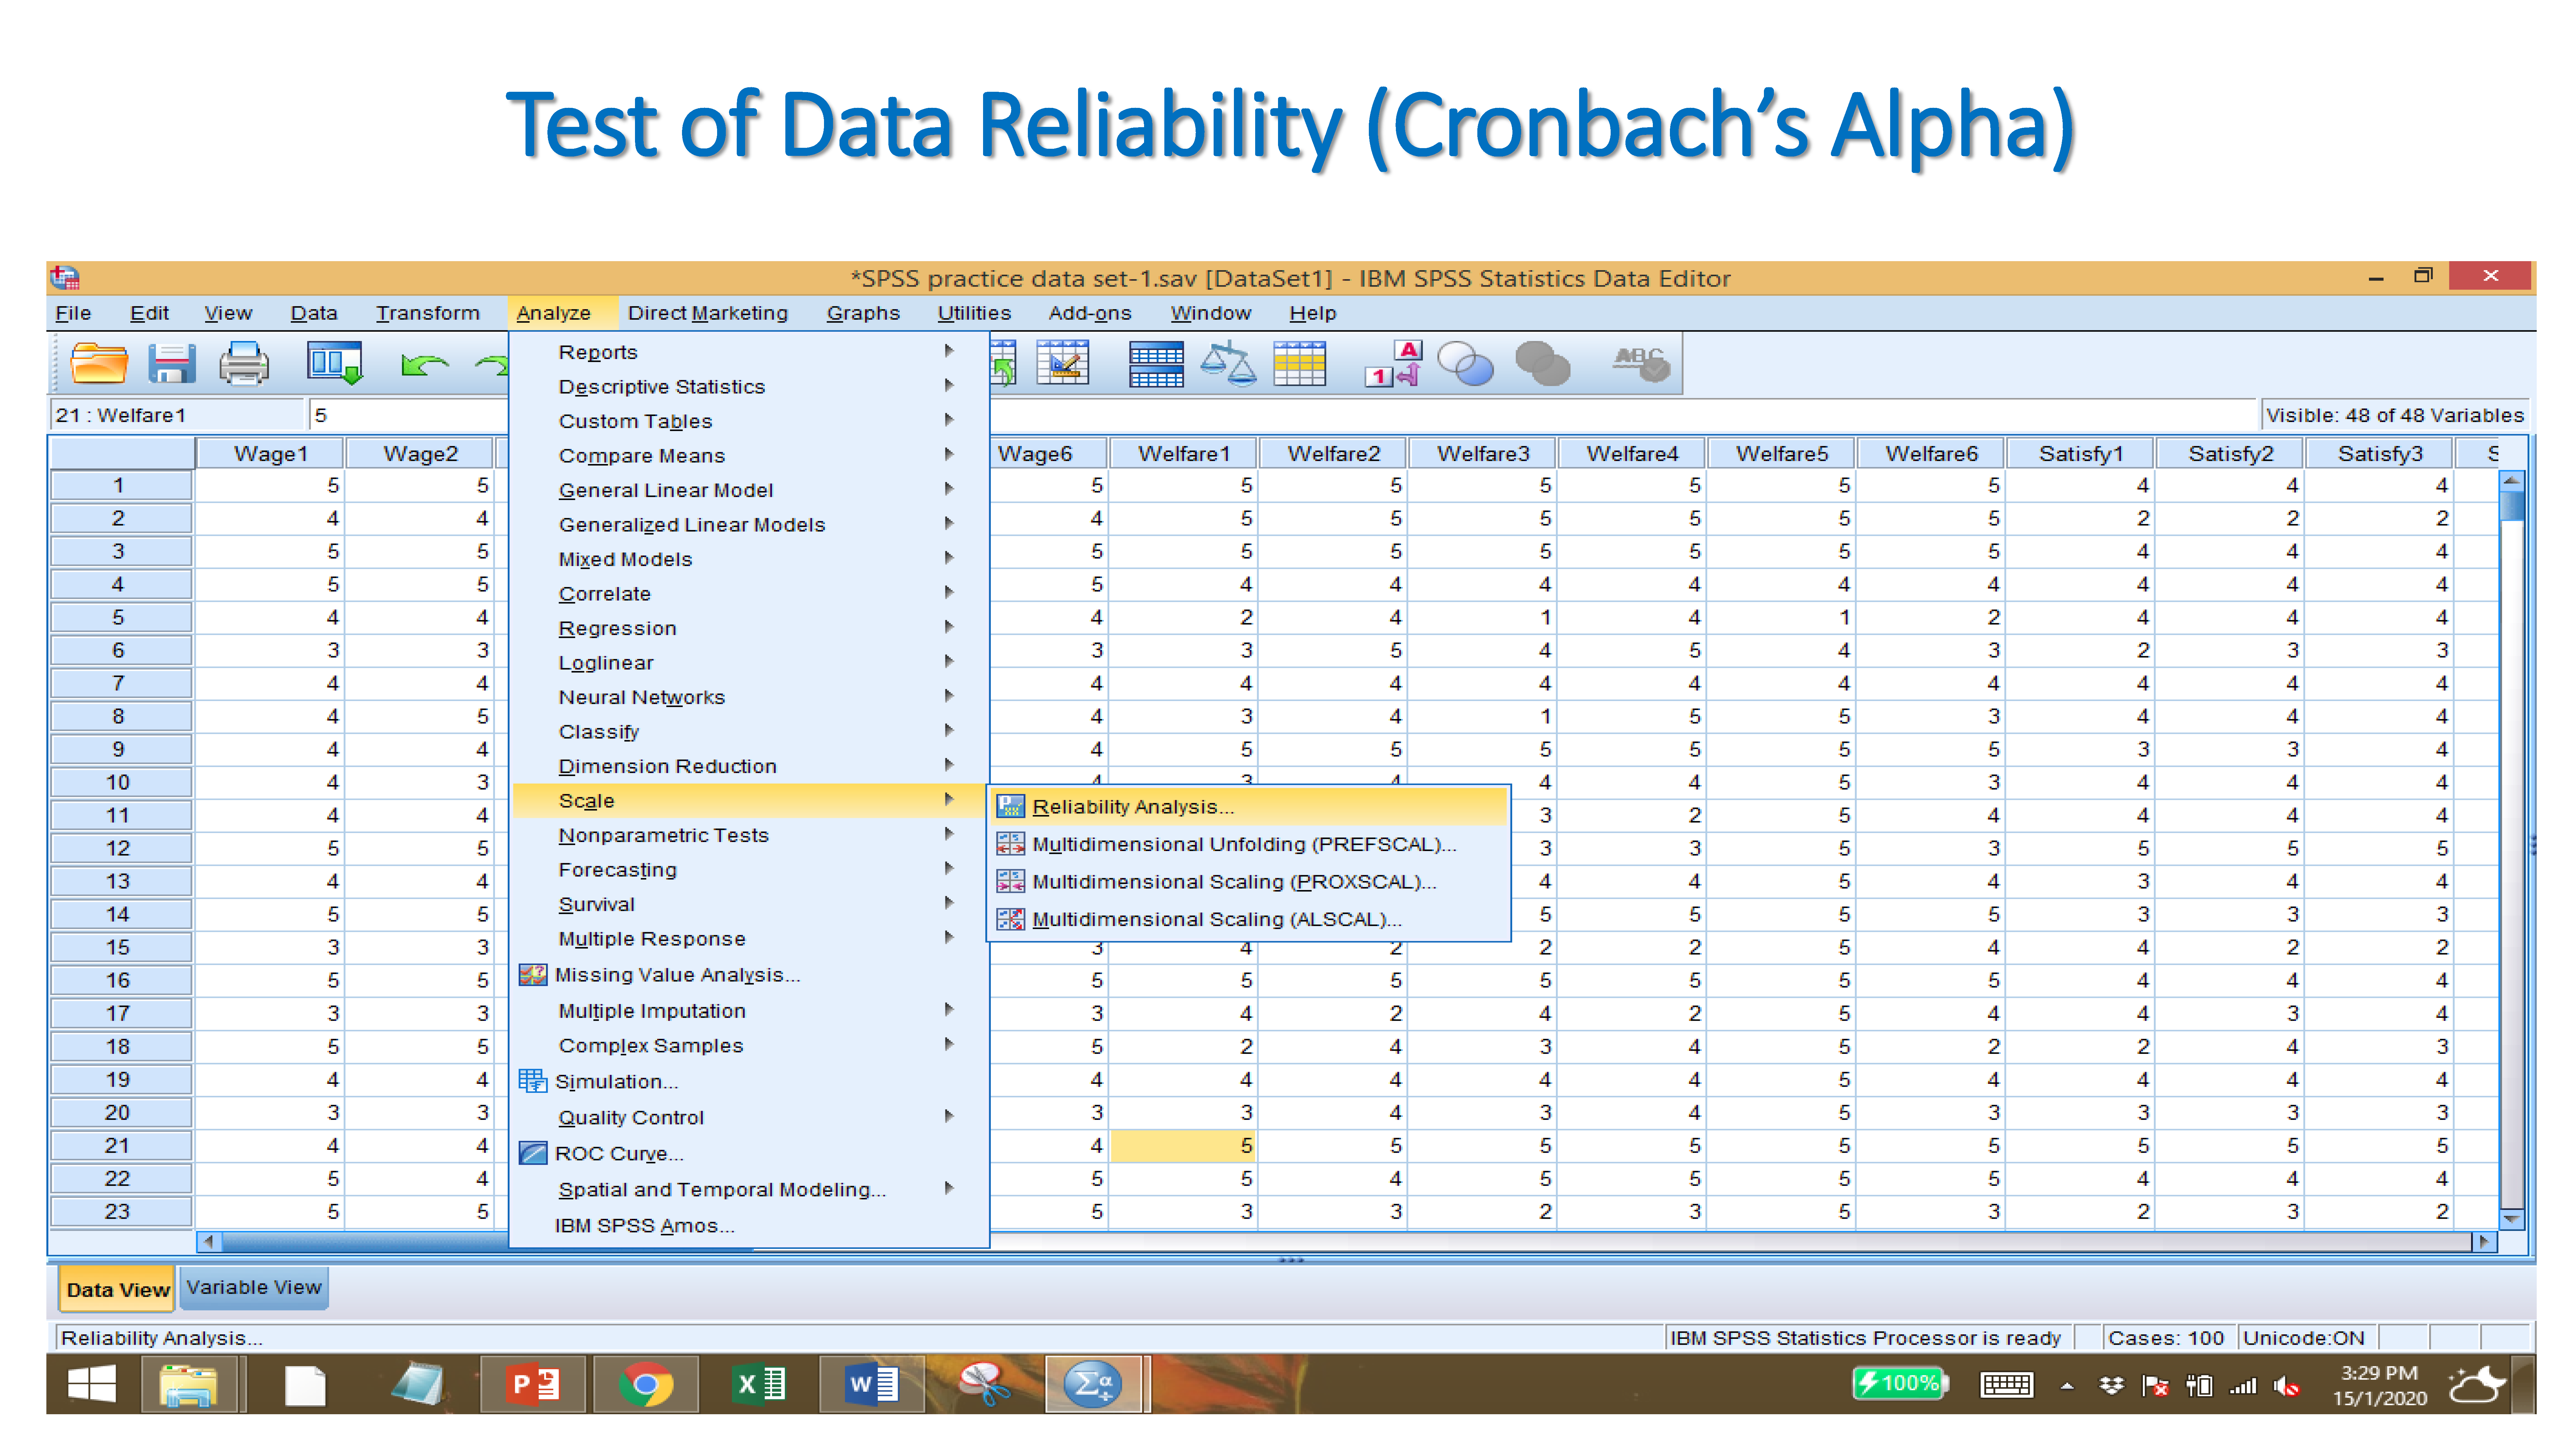
\includegraphics{images/slides/img_Page_062.png}

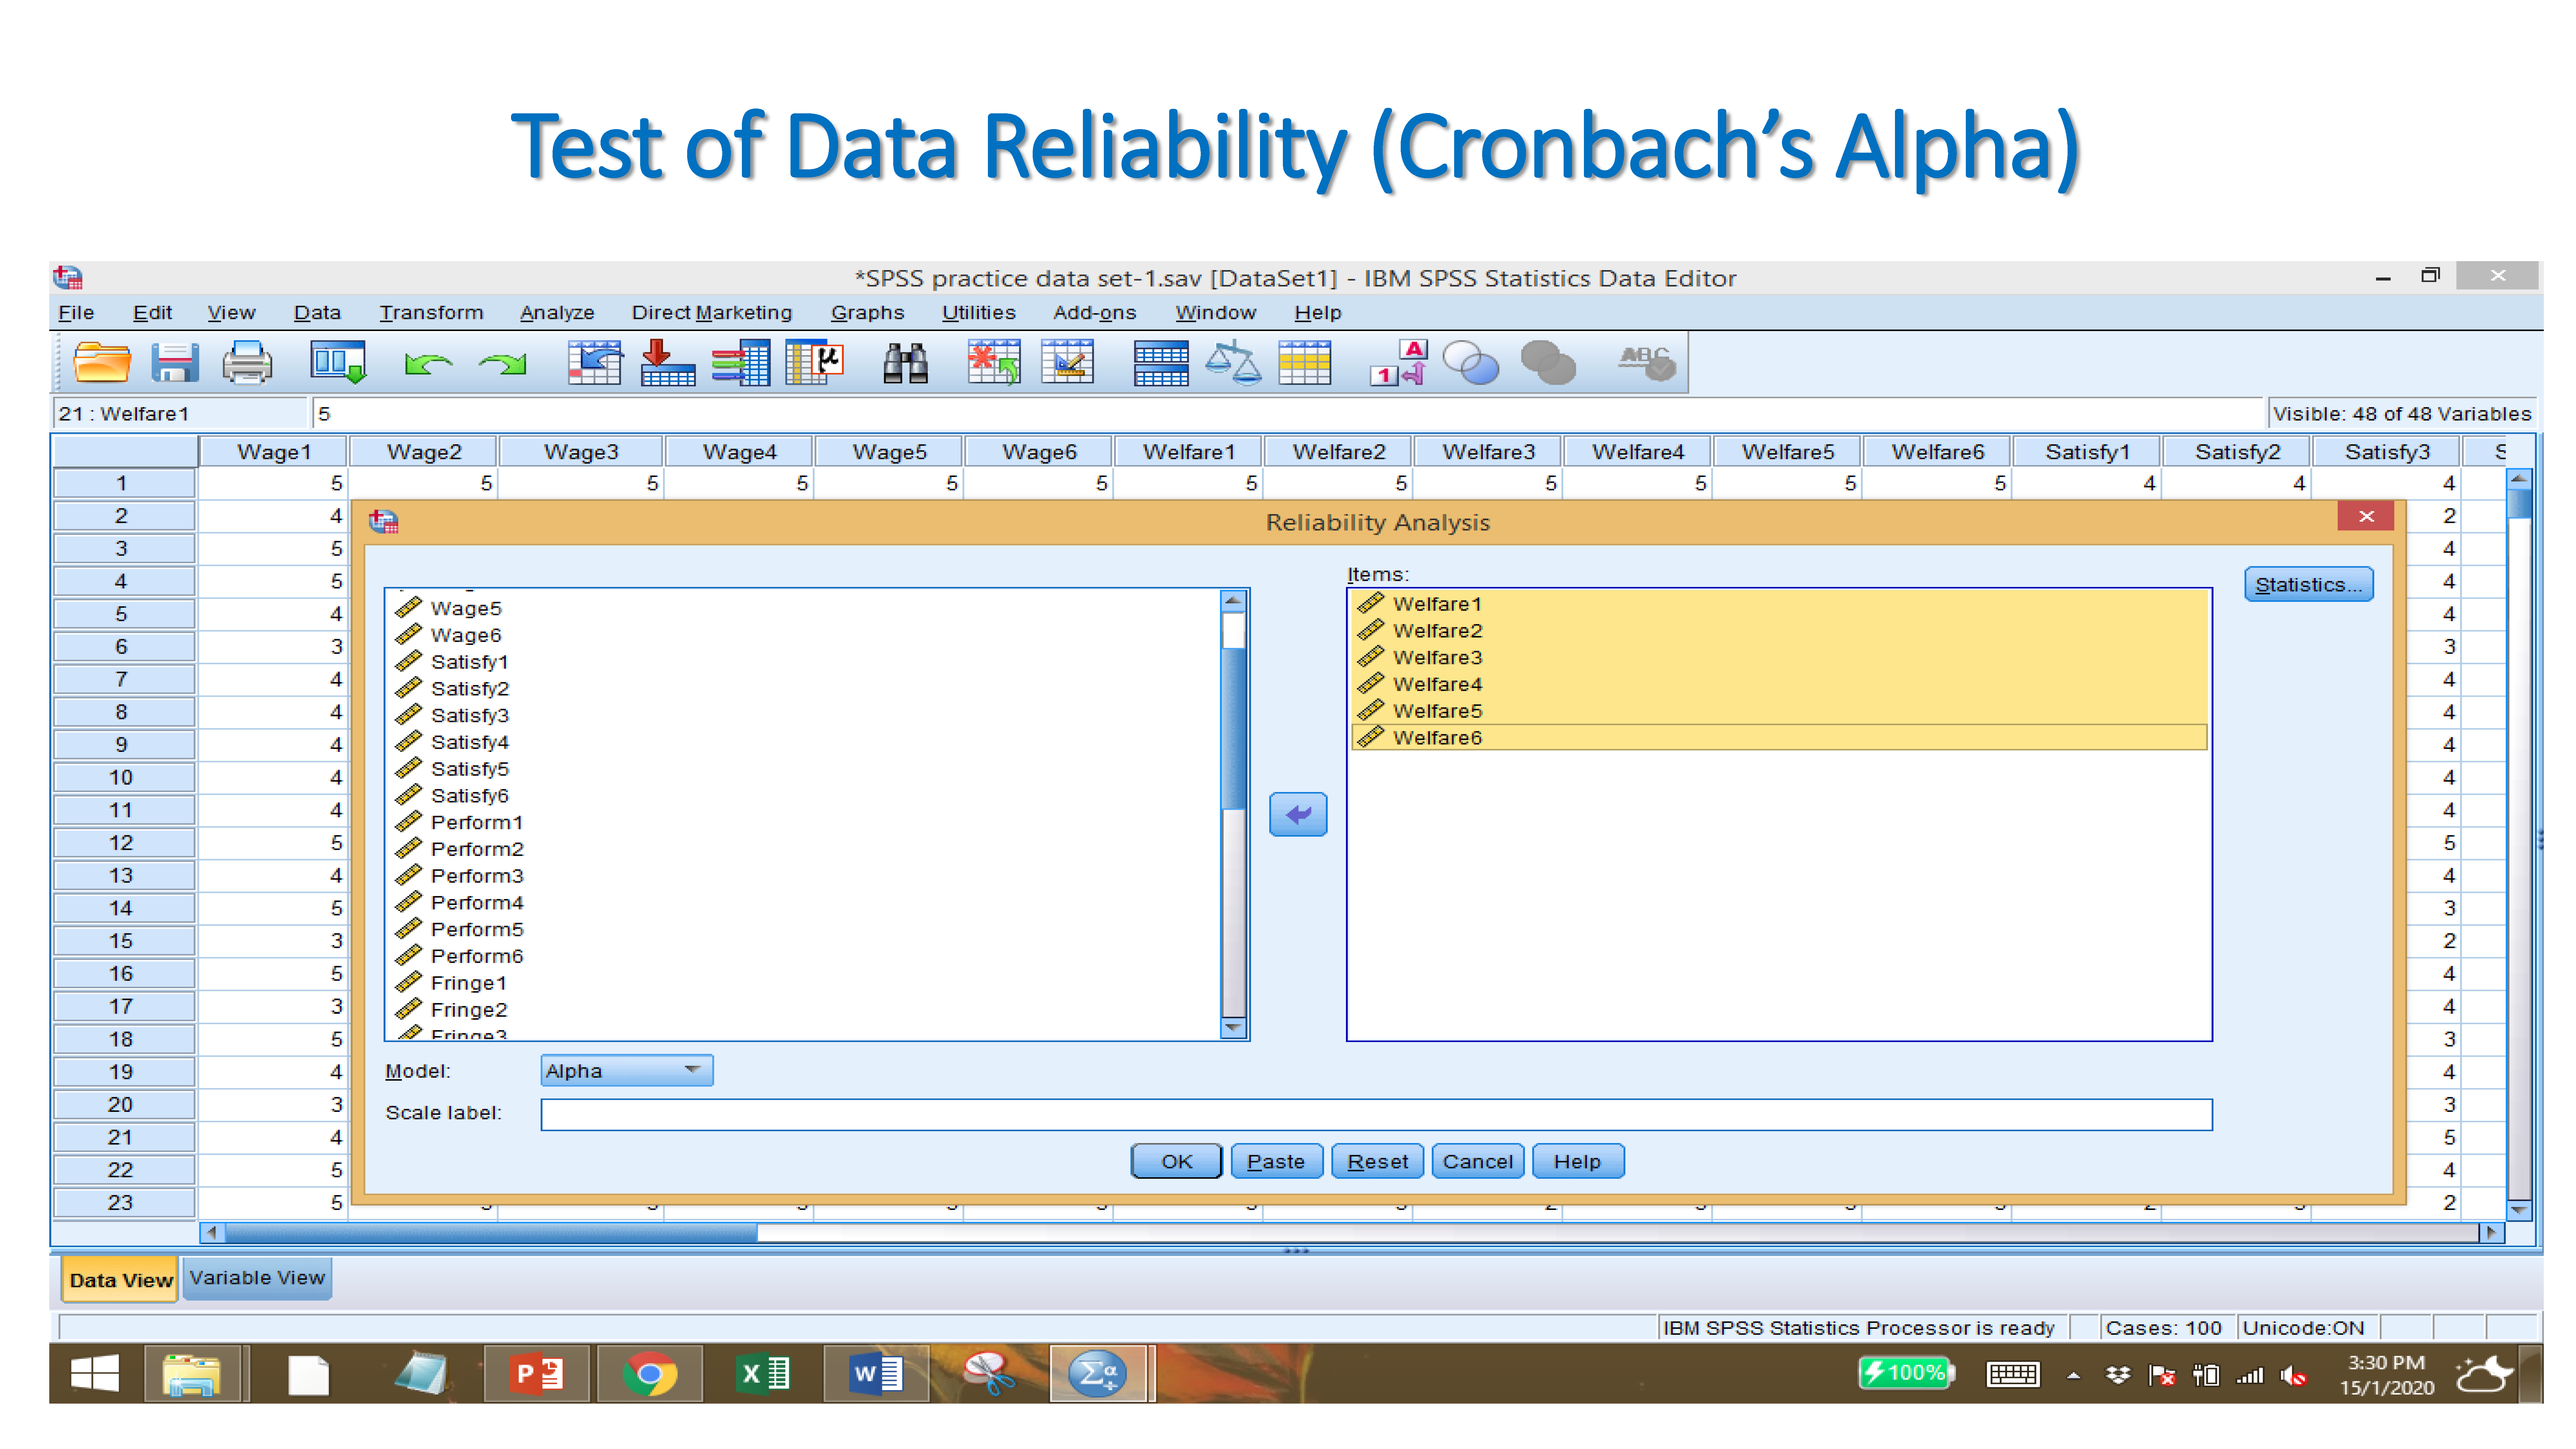
\includegraphics{images/slides/img_Page_063.png}

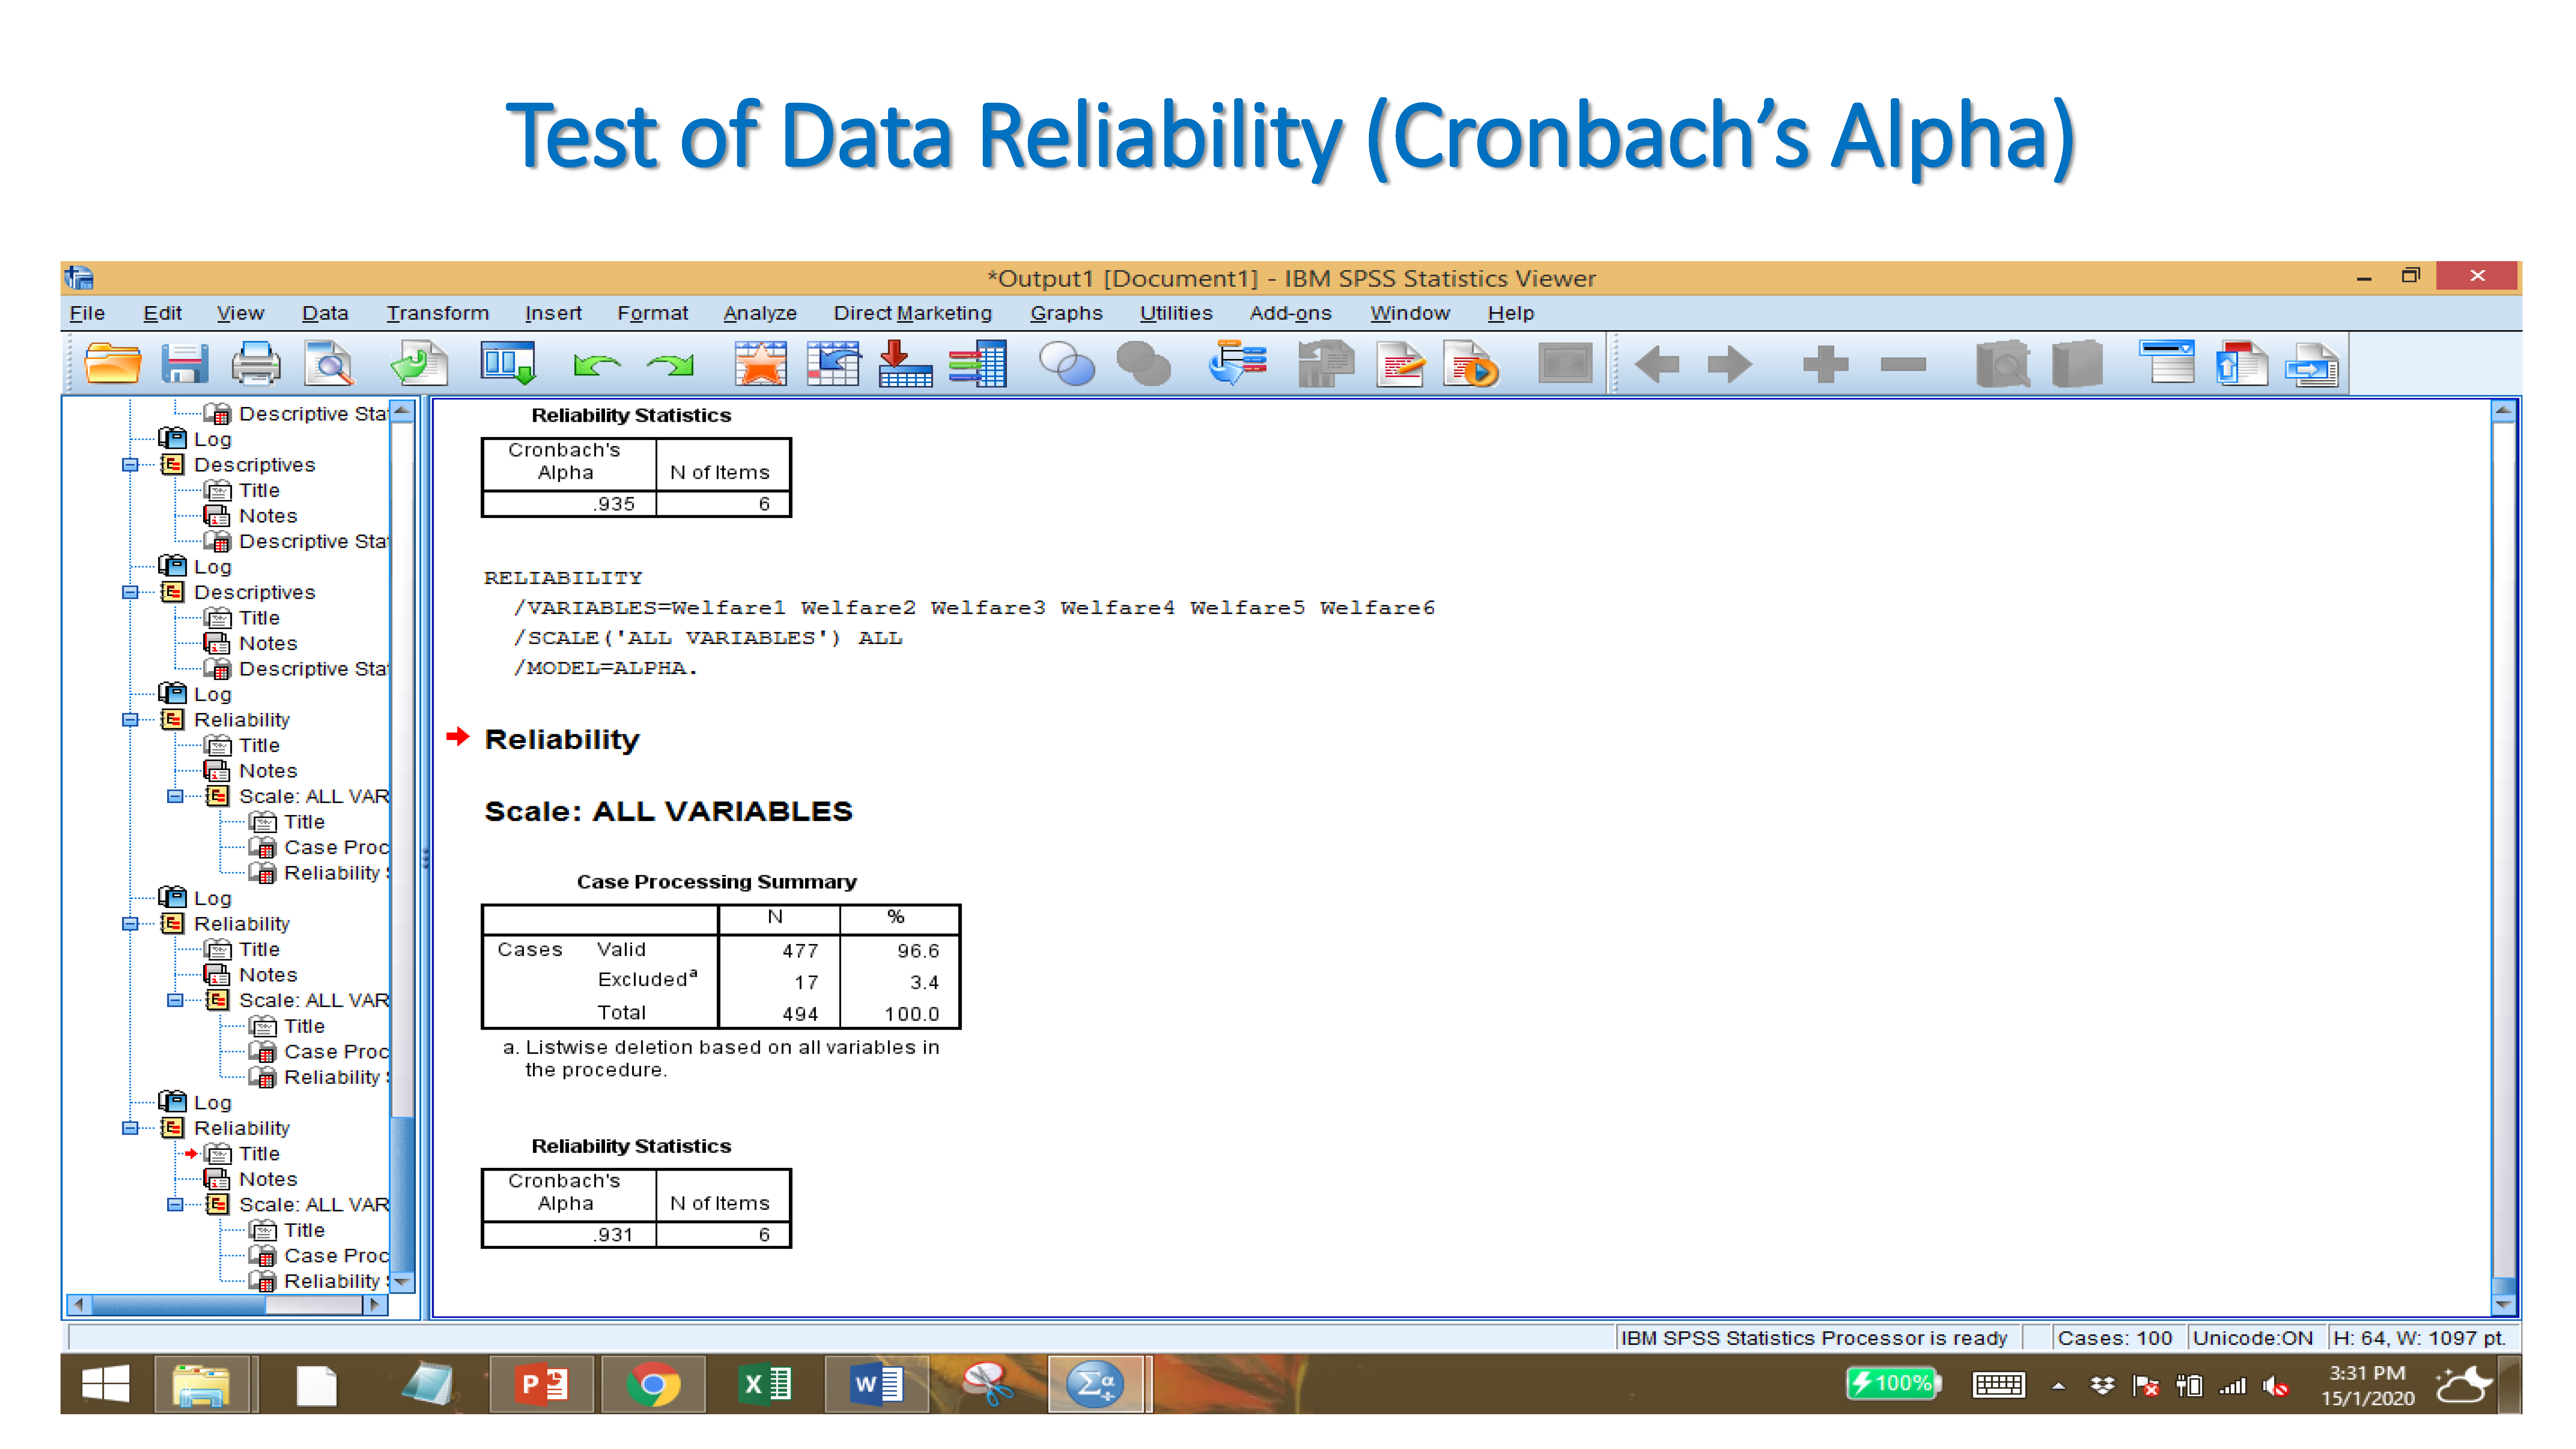
\includegraphics{images/slides/img_Page_064.png}

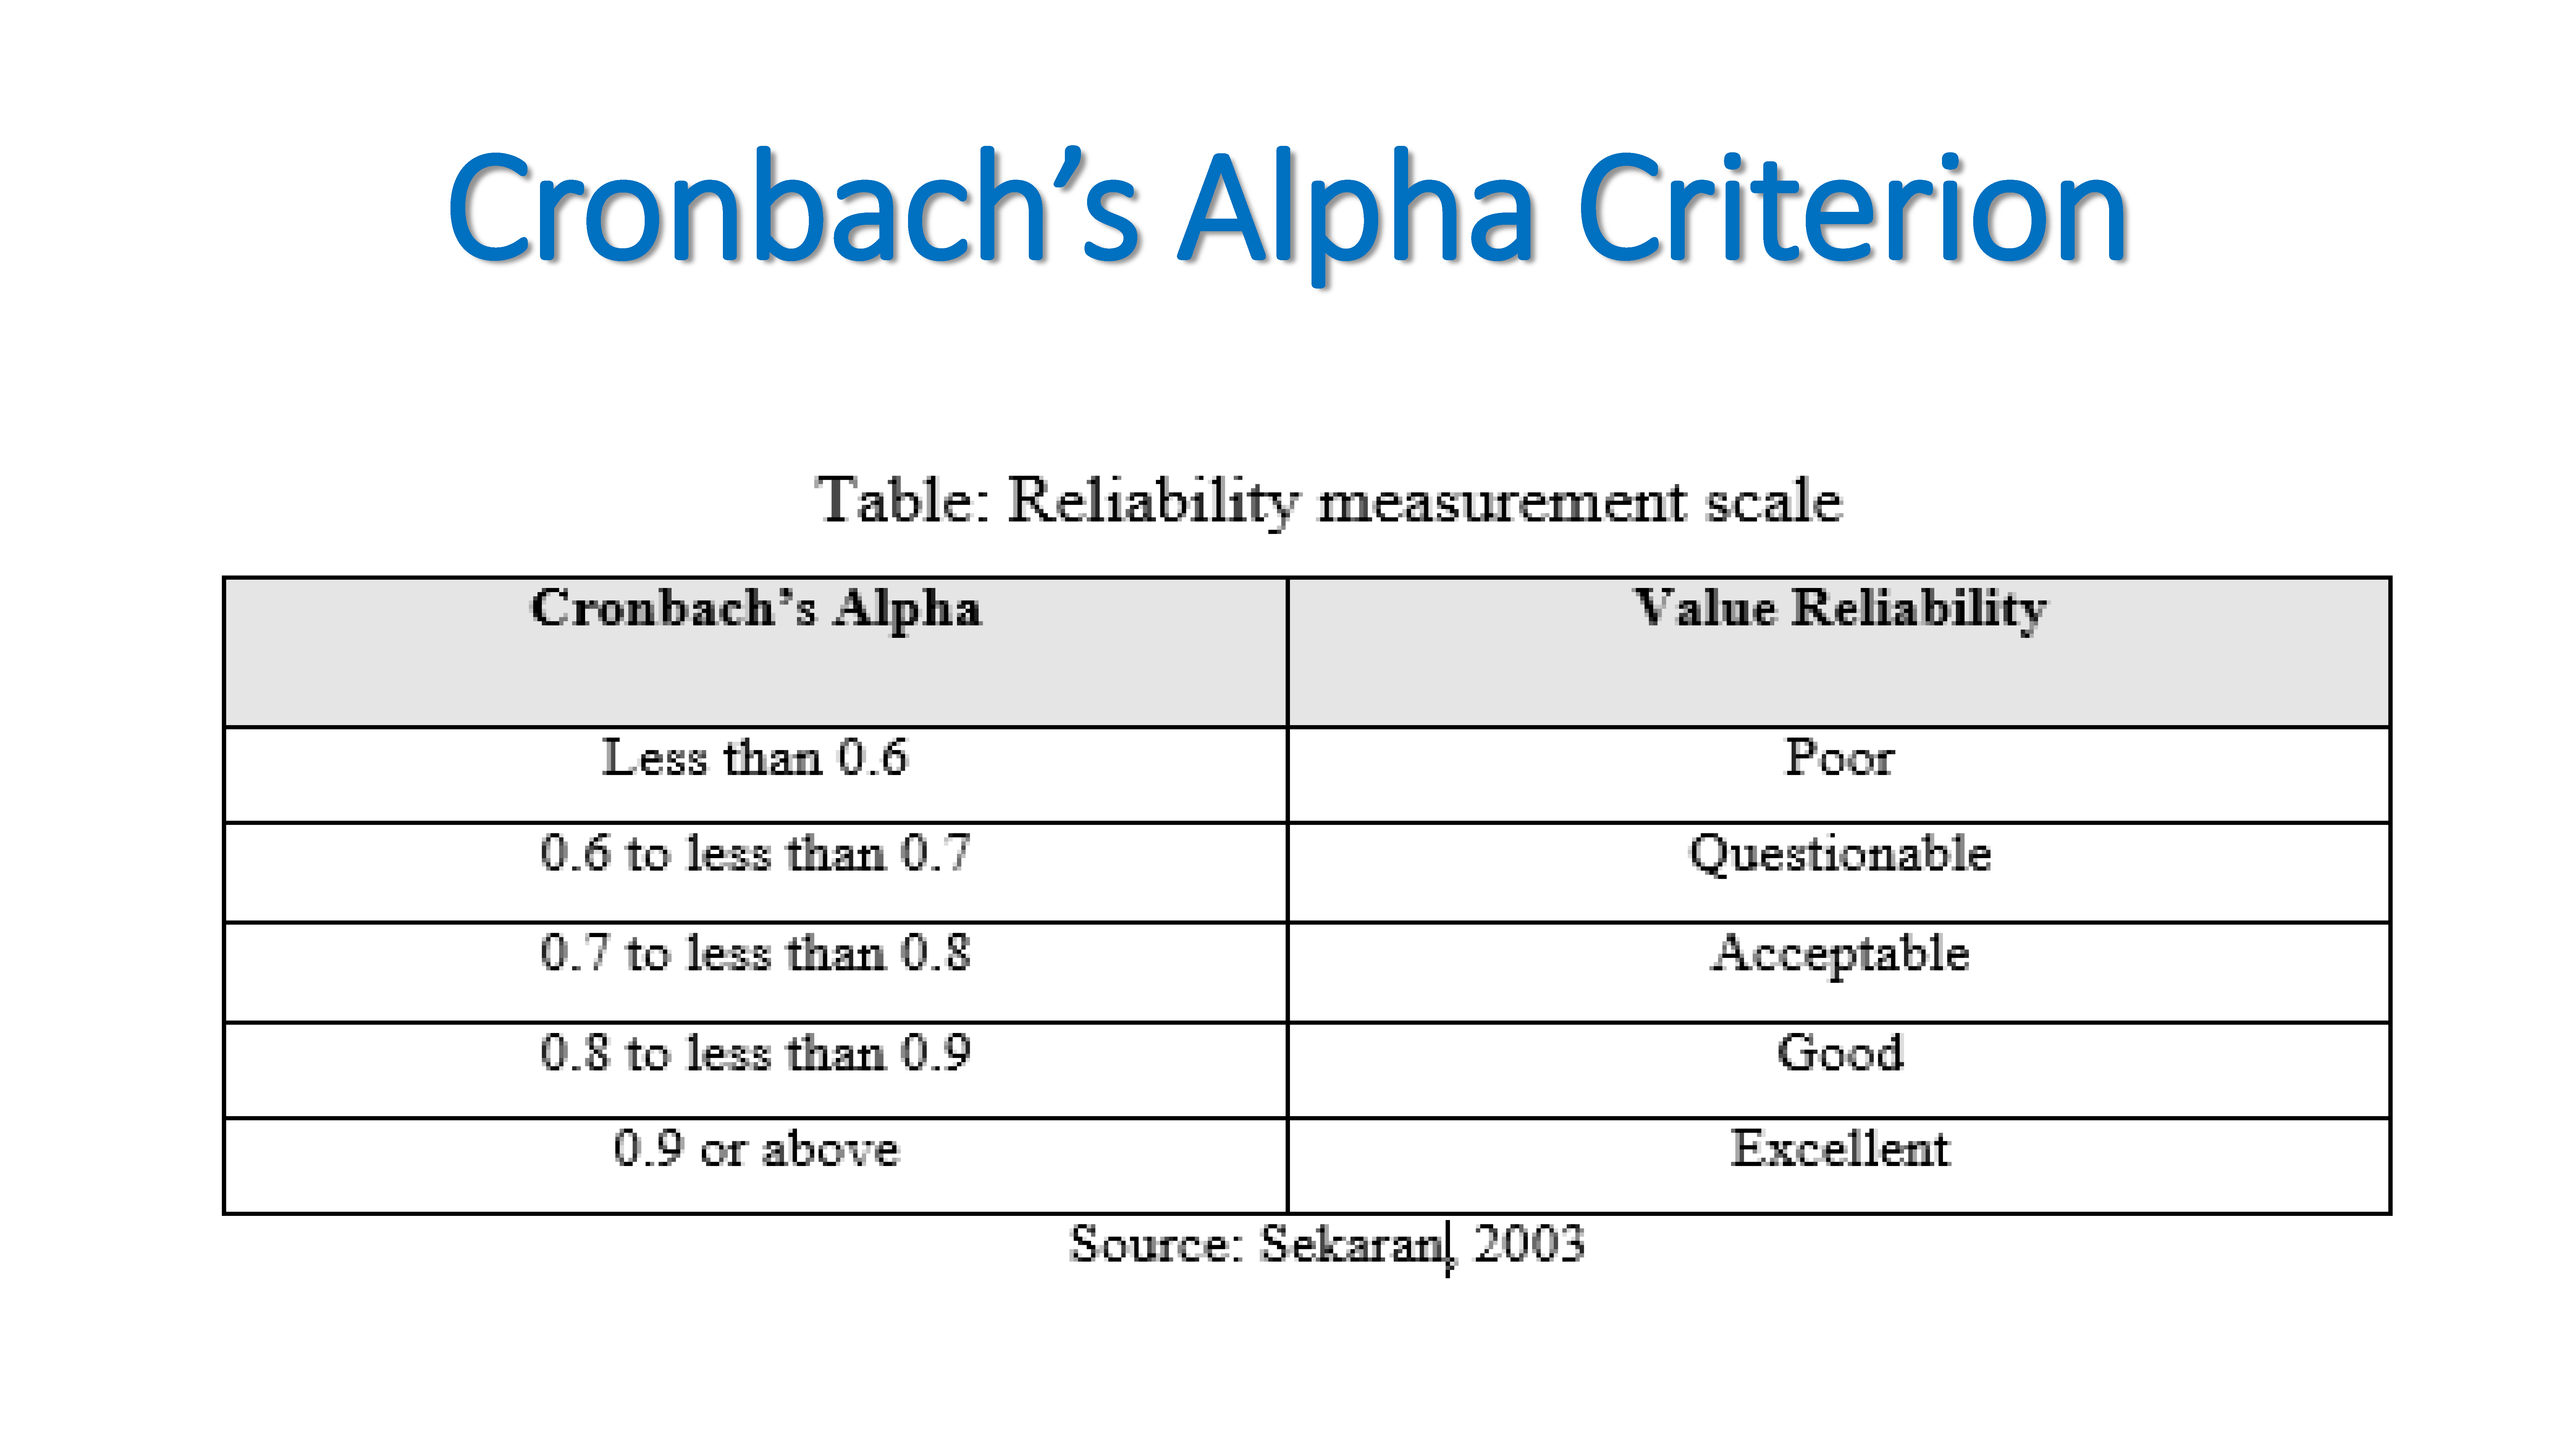
\includegraphics{images/slides/img_Page_065.png}

\bookmarksetup{startatroot}

\chapter{Exploratory Factor Analysis
(EFA)}\label{exploratory-factor-analysis-efa}

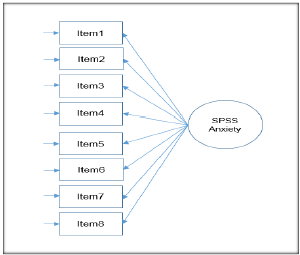
\includegraphics{images/efa.png}

In multivariate statistics, exploratory factor analysis (EFA) is a
statistical method used to uncover the underlying structure of a
relatively large set of variables. EFA is a technique within factor
analysis whose overarching goal is to identify the underlying
relationships between measured variables.\\

{\textbf{Assumption:}}\\

\begin{itemize}
\tightlist
\item
  Data must be Interval or Ratio measurement scale. E.g. Likert scale
  data or grouped data (1,2,3,4,5,6,7 point scale data).\\
\item
  Sample size must at least 4/5 times of variables.\\
\item
  Correlation Matrix: if values are near to +/- 1, and more than +.5 or
  -.5 these variable counts.\\
\item
  KMO test: if value more than .5\\
\item
  Bartlett's test: if value sig. value smaller than .05 or .01.\\
\item
  Eigenvalues: components or variables having value 1 and more than 1.\\
\item
  Factor loading: if values exit in factors loading (item value more
  than .5).\\
\item
  Multicollinearity: If in correlation matrix two items value is .80 or
  above, there is multicollinearity. Having same line, lying is the same
  lining.\\
\item
  Communality (component matrix): if value is near 1 or more than
  70-80\% (considered)- Scree plot: it show value more than 1.\\
\end{itemize}

\includegraphics{images/slides/img_Page_068.png}

\includegraphics{images/slides/img_Page_069.png}

\includegraphics{images/slides/img_Page_070.png}

\includegraphics{images/slides/img_Page_071.png}

\includegraphics{images/slides/img_Page_072.png}

\includegraphics{images/slides/img_Page_073.png}

\includegraphics{images/slides/img_Page_074.png}

\includegraphics{images/slides/img_Page_075.png}

\includegraphics{images/slides/img_Page_076.png}

\includegraphics{images/slides/img_Page_077.png}

\includegraphics{images/slides/img_Page_078.png}

\includegraphics{images/slides/img_Page_079.png}

\includegraphics{images/slides/img_Page_080.png}

\bookmarksetup{startatroot}

\chapter{Testing of means}\label{testing-of-means}

Testing of means: This analysis illustrates that whether there is
difference between two groups or among three group and it is
significant.\\

Two Assumptions:\\

\begin{enumerate}
\def\labelenumi{\arabic{enumi}.}
\tightlist
\item
  If data does not come from normal distribution or sample size is small
  meaning that less than 30 then nonparametric test.\\
\item
  If data comes from large and normal distribution, then parametric
  test.\\
\end{enumerate}

\section{Non Parametric}\label{non-parametric}

{Assumption:}\\

When data are not normally distributed then non parametric test is
done.\\

\begin{itemize}
\tightlist
\item
  Sample size is small (less than 30)\\
\item
  Data are not from normally distributing\\
\item
  When data is not normal any way\\
\item
  Regular statistics can't be done\\
\end{itemize}

\includegraphics{images/non-para.png}

\section{Parametric}\label{parametric}

{Assumptions:}\\

If data comes from large and normal distribution, then parametric
test.\\

{Parametric Tests:}\\

A. One sample test\\
B. Two sample test\\
- Independent sample `t' test\\
- Paired sample `t' test\\
C. More than two sample test (ANOVA)\\

\subsection{One-sample t-test}\label{one-sample-t-test}

\begin{itemize}
\tightlist
\item
  The One Sample t Test compares a sample mean to a hypothesized
  population mean to determine whether the two means are significantly
  different.\\
\item
  The One Sample t Test determines whether the sample mean is
  statistically different from a known or hypothesized population mean.
  The One Sample t Test is a parametric test.\\
\item
  This test is also known as: {Single Sample t Test}\\
\item
  The variable used in this test is known as: {Test variable}\\
\item
  In a One Sample t Test, the test variable is compared against a ``test
  value'', which is a known or hypothesized value of the mean in the
  population.\\
\end{itemize}

{The One Sample t-test determines whether the sample mean is
statistically different from a known or hypothesized population mean.}\\

{The sample data must comply three conditions}\\

{1. Scale data\\
2. Normally distributed data\\
3. Only one sample data\\
}\strut \\

\textbf{Example of one-sample t-test}\\

We assume that the hypothesized population mean is 3.\\

\begin{tcolorbox}[enhanced jigsaw, rightrule=.15mm, arc=.35mm, colframe=quarto-callout-note-color-frame, coltitle=black, left=2mm, colbacktitle=quarto-callout-note-color!10!white, bottomtitle=1mm, titlerule=0mm, colback=white, breakable, opacitybacktitle=0.6, opacityback=0, toprule=.15mm, toptitle=1mm, title=\textcolor{quarto-callout-note-color}{\faInfo}\hspace{0.5em}{Hypothesis}, bottomrule=.15mm, leftrule=.75mm]

Null Hypothesis: The sample mean is not significantly different from the
hypothesized population mean\\
Alternative Hypothesis: The sample mean is significantly different from
the hypothesized population mean\\

\end{tcolorbox}

If p (sig value) is less than 0.05, then we reject the null
hypothesis.\\

\includegraphics{images/slides/img_Page_087.png}

\includegraphics{images/slides/img_Page_088.png}

\includegraphics{images/slides/img_Page_089.png}

\includegraphics{images/slides/img_Page_090.png}

\includegraphics{images/slides/img_Page_091.png}

\begin{tcolorbox}[enhanced jigsaw, rightrule=.15mm, arc=.35mm, colframe=quarto-callout-note-color-frame, coltitle=black, left=2mm, colbacktitle=quarto-callout-note-color!10!white, bottomtitle=1mm, titlerule=0mm, colback=white, breakable, opacitybacktitle=0.6, opacityback=0, toprule=.15mm, toptitle=1mm, title=\textcolor{quarto-callout-note-color}{\faInfo}\hspace{0.5em}{Decision}, bottomrule=.15mm, leftrule=.75mm]

Since the significant value less than 0.05 which means we reject the
null hypothesis. It indicates that sample mean is significantly
different from the hypothesized population mean.

\end{tcolorbox}

\subsection{Independent Sample t-Test}\label{independent-sample-t-test}

The Independent Samples t Test compares the means of two independent
groups in order to determine whether there is statistical evidence that
the associated population means are significantly different. The
Independent Samples t Test is a parametric test.\\

\includegraphics{images/ind-t-test.png}

\begin{tcolorbox}[enhanced jigsaw, rightrule=.15mm, arc=.35mm, colframe=quarto-callout-note-color-frame, coltitle=black, left=2mm, colbacktitle=quarto-callout-note-color!10!white, bottomtitle=1mm, titlerule=0mm, colback=white, breakable, opacitybacktitle=0.6, opacityback=0, toprule=.15mm, toptitle=1mm, title=\textcolor{quarto-callout-note-color}{\faInfo}\hspace{0.5em}{Hypothesis}, bottomrule=.15mm, leftrule=.75mm]

{Null hypothesis:} {There is no significant difference between male and
female towards GPA score.}\\
\strut \\
{Alternate hypothesis:} {There is a significant difference between male
and female towards GPA score.}\\

\end{tcolorbox}

After Importing your data set, and providing names to variables, click
on:\\

{ANALYZE → COMPARE MEANS → INDEPENDENT SAMPLES T TEST}

T-TEST\\

\begin{itemize}
\tightlist
\item
  For TEST VARIABLE, Select the dependent variable (GPA)\\
\item
  For GROUPING VARIABLE, Select the independent variable (Gender)\\
\end{itemize}

\includegraphics{images/slides/img_Page_096.png}

\includegraphics{images/slides/img_Page_097.png}

\includegraphics{images/slides/img_Page_098.png}

\includegraphics{images/slides/img_Page_099.png}

\begin{tcolorbox}[enhanced jigsaw, rightrule=.15mm, arc=.35mm, colframe=quarto-callout-note-color-frame, coltitle=black, left=2mm, colbacktitle=quarto-callout-note-color!10!white, bottomtitle=1mm, titlerule=0mm, colback=white, breakable, opacitybacktitle=0.6, opacityback=0, toprule=.15mm, toptitle=1mm, title=\textcolor{quarto-callout-note-color}{\faInfo}\hspace{0.5em}{Decision}, bottomrule=.15mm, leftrule=.75mm]

Since the significant value of P is less than 0.05 which is 0.011. It
indicates that null hypothesis is rejected which refereeing that there
is a significant difference between male and female for obtaining GPA
score.\\

\includegraphics{images/ind-t-test-out1.png}

\end{tcolorbox}

\subsection{Paired Samples T -test.}\label{paired-samples-t--test.}

\begin{itemize}
\tightlist
\item
  SPSS paired samples t-test is a procedure for testing whether the
  means of two metric variables are equal in same population. Both
  variables have been measured on the same cases.\\
\item
  Although ``paired samples'' suggests that multiple samples are
  involved, there's really only one sample and two variables.\\
\item
  Below is the pre-test and post-test scores of a training program.\\
\end{itemize}

\includegraphics{images/paired-t-test.png}

\begin{tcolorbox}[enhanced jigsaw, rightrule=.15mm, arc=.35mm, colframe=quarto-callout-note-color-frame, coltitle=black, left=2mm, colbacktitle=quarto-callout-note-color!10!white, bottomtitle=1mm, titlerule=0mm, colback=white, breakable, opacitybacktitle=0.6, opacityback=0, toprule=.15mm, toptitle=1mm, title=\textcolor{quarto-callout-note-color}{\faInfo}\hspace{0.5em}{Hypothesis}, bottomrule=.15mm, leftrule=.75mm]

{Null hypothesis:} {There is no significant difference between pretest
score and post-test score.}\\
\strut \\
{Alternate hypothesis:} {There is a significant difference between
pre-test score and post-test score.}\\

\end{tcolorbox}

After Importing your data set, and providing names to variables, click
on:\\

{ANALYZE → COMPARE MEANS → PAIRED SAMPLES T TEST}

For PAIRED VARIABLES, Select the two dependent (response) variables (the
analysis will be based on first variable minus second variable)\\

\includegraphics{images/slides/img_Page_104.png}

\includegraphics{images/slides/img_Page_105.png}

\includegraphics{images/slides/img_Page_106.png}

\begin{tcolorbox}[enhanced jigsaw, rightrule=.15mm, arc=.35mm, colframe=quarto-callout-note-color-frame, coltitle=black, left=2mm, colbacktitle=quarto-callout-note-color!10!white, bottomtitle=1mm, titlerule=0mm, colback=white, breakable, opacitybacktitle=0.6, opacityback=0, toprule=.15mm, toptitle=1mm, title=\textcolor{quarto-callout-note-color}{\faInfo}\hspace{0.5em}{Results Observation}, bottomrule=.15mm, leftrule=.75mm]

Since the sig value (\emph{p}) is less than 0.05 which is 0.000 that
means null hypothesis is rejected and alternate hypothesis is accepted.
It indicates that there is a significant difference of training scores
between pre-test and post-test.\\
\strut \\
\includegraphics{images/paired-t-test-out1.png}

\end{tcolorbox}

\subsection{One-way ANOVA}\label{one-way-anova}

\hfill\break
The one-way analysis of variance (ANOVA) is used to determine whether
there are any statistically significant differences between the means of
three or more independent (unrelated) groups.\\
\strut \\
\textbf{Example of one-way ANOVA}\\

\includegraphics{images/anova.png}

There are three teaching method which are traditional, machine learning
and both traditional \& M.L method. The scores obtained by students
under these three teaching method. Now, one-way ANOVA is used to
determine whether there are any statistically significant differences
among the scores obtained by these three methods.

\includegraphics{images/slides/img_Page_110.png}

\includegraphics{images/slides/img_Page_111.png}

\includegraphics{images/slides/img_Page_112.png}

\begin{tcolorbox}[enhanced jigsaw, rightrule=.15mm, arc=.35mm, colframe=quarto-callout-note-color-frame, coltitle=black, left=2mm, colbacktitle=quarto-callout-note-color!10!white, bottomtitle=1mm, titlerule=0mm, colback=white, breakable, opacitybacktitle=0.6, opacityback=0, toprule=.15mm, toptitle=1mm, title=\textcolor{quarto-callout-note-color}{\faInfo}\hspace{0.5em}{Results Observation}, bottomrule=.15mm, leftrule=.75mm]

\hfill\break
The sig value for between groups is higher than 0.05 that indicates to
accept null hypothesis. Similarly, pairwise result also showed
insignificant.\\
\strut \\
\includegraphics{images/anova-out1.png}

\end{tcolorbox}

\subsection{Two-way ANOVA}\label{two-way-anova}

\hfill\break
A test that allows one to make comparisons between the means of three or
more groups of data, where two independent variables are considered.
Two-Way ANOVA is an extension to the one-way ANOVA.\\
\strut \\
\textbf{Example of Two-way ANOVA}\\
\strut \\

\includegraphics{images/two-way-anova.png}

For example, family members, income, and expenditure are the three
variables. Family members and income are the independent variables and
nominal data. Expenditure is dependent variable and scale data. So, we
will observe here;\\
\strut \\
1. Is there any significant differences of amount of monthly income and
amount of monthly expenditure on shampoo purchase?\\
2. Is there any significant difference between number of family members
in house and expenditure on shampoo purchase?\\

\begin{tcolorbox}[enhanced jigsaw, rightrule=.15mm, arc=.35mm, colframe=quarto-callout-note-color-frame, coltitle=black, left=2mm, colbacktitle=quarto-callout-note-color!10!white, bottomtitle=1mm, titlerule=0mm, colback=white, breakable, opacitybacktitle=0.6, opacityback=0, toprule=.15mm, toptitle=1mm, title=\textcolor{quarto-callout-note-color}{\faInfo}\hspace{0.5em}{Hypothesis to test by Two-way ANOVA}, bottomrule=.15mm, leftrule=.75mm]

Null hypothesis 1: \emph{Amount of monthly expenditure on shampoo for
different income do not differ}\\

Null hypothesis 2: \emph{Amount of monthly expenditure on shampoo for
different number of family members in house do not differ}\\

Null hypothesis 3: \emph{Amount of monthly expenditure on shampoo for
the interaction of income and number of family members do not differ}\\

\end{tcolorbox}

\includegraphics{images/slides/img_Page_117.png}

\includegraphics{images/slides/img_Page_118.png}

\begin{tcolorbox}[enhanced jigsaw, rightrule=.15mm, arc=.35mm, colframe=quarto-callout-note-color-frame, coltitle=black, left=2mm, colbacktitle=quarto-callout-note-color!10!white, bottomtitle=1mm, titlerule=0mm, colback=white, breakable, opacitybacktitle=0.6, opacityback=0, toprule=.15mm, toptitle=1mm, title=\textcolor{quarto-callout-note-color}{\faInfo}\hspace{0.5em}{Results Observation}, bottomrule=.15mm, leftrule=.75mm]

Since the income and family members with expenditure values are more
than 0.05, therefore null hypothesis are accepted. However, for
intercept null hypothesis is rejected as the p value is less than 0.05\\

\includegraphics{images/two-way-anova-out1.png}

\end{tcolorbox}

\subsection{One-way Repeated Measure
ANOVA}\label{one-way-repeated-measure-anova}

\hfill\break
One-Way Repeated-Measures ANOVA. Analysis of Variance (ANOVA) is a
common and robust statistical test that you can use to compare the mean
scores collected from different conditions or groups in an experiment.\\
\strut \\
\includegraphics{images/slides/img_Page_121.png}

\begin{tcolorbox}[enhanced jigsaw, rightrule=.15mm, arc=.35mm, colframe=quarto-callout-note-color-frame, coltitle=black, left=2mm, colbacktitle=quarto-callout-note-color!10!white, bottomtitle=1mm, titlerule=0mm, colback=white, breakable, opacitybacktitle=0.6, opacityback=0, toprule=.15mm, toptitle=1mm, title=\textcolor{quarto-callout-note-color}{\faInfo}\hspace{0.5em}{Hypothesis}, bottomrule=.15mm, leftrule=.75mm]

{Null Hypothesis:} There is no significant difference among the three
different teaching methods.\\
{Alternative Hypothesis:} There is a significant difference among the
three different teaching methods.\\

\end{tcolorbox}

\includegraphics{images/slides/img_Page_123.png}

\includegraphics{images/slides/img_Page_124.png}

\includegraphics{images/slides/img_Page_125.png}

\includegraphics{images/slides/img_Page_126.png}

\begin{tcolorbox}[enhanced jigsaw, rightrule=.15mm, arc=.35mm, colframe=quarto-callout-note-color-frame, coltitle=black, left=2mm, colbacktitle=quarto-callout-note-color!10!white, bottomtitle=1mm, titlerule=0mm, colback=white, breakable, opacitybacktitle=0.6, opacityback=0, toprule=.15mm, toptitle=1mm, title=\textcolor{quarto-callout-note-color}{\faInfo}\hspace{0.5em}{Results Observation}, bottomrule=.15mm, leftrule=.75mm]

Since the p-value is \textless.05. The null hypothesis is rejected.
Therefore, we can say there is significant difference among the teaching
methods.\\

\includegraphics{images/one-way-repeat-out1.png}

\end{tcolorbox}

\bookmarksetup{startatroot}

\chapter{Correlation Tests}\label{correlation-tests}

Correlation is a statistical technique that shows how strongly two
variables are related to each other or the degree of association between
the two\\

\includegraphics{images/slides/img_Page_130.png}

\includegraphics{images/slides/img_Page_131.png}

\includegraphics{images/slides/img_Page_132.png}

\includegraphics{images/slides/img_Page_133.png}

\begin{tcolorbox}[enhanced jigsaw, rightrule=.15mm, arc=.35mm, colframe=quarto-callout-note-color-frame, coltitle=black, left=2mm, colbacktitle=quarto-callout-note-color!10!white, bottomtitle=1mm, titlerule=0mm, colback=white, breakable, opacitybacktitle=0.6, opacityback=0, toprule=.15mm, toptitle=1mm, title=\textcolor{quarto-callout-note-color}{\faInfo}\hspace{0.5em}{Correlation Decision Criteria}, bottomrule=.15mm, leftrule=.75mm]

If r = from 0.75 to 0.95\\
Result: highly positive linear correlation\\
\strut \\
If r = from 0.50 to 0.75\\
Result: medium positive linear correlation\\
\strut \\
If r = from 0.25 to 0.50\\
Result: slight positive linear correlation\\
\strut \\
If r = from 0.10 to 0.25\\
Result: Weak positive linear correlation\\

\end{tcolorbox}

\bookmarksetup{startatroot}

\chapter{Regression Analysis}\label{regression-analysis}

In statistical modelling, regression analysis is a set of statistical
processes for estimating the relationships between a dependent variable
and one or more independent variables.\\

\section{Simple Linear Regression}\label{simple-linear-regression}

\begin{itemize}
\tightlist
\item
  Linear regression models are used to show or predict the relationship
  between two variables or factors. The factor that is being predicted
  (the factor that the equation solves for) is called the dependent
  variable. The factors that are used to predict the value of the
  dependent variable are called the independent variables.\\
\item
  The simplest form of a regression analysis uses one dependent variable
  and one independent variable.\\
\end{itemize}

\includegraphics{images/slides/img_Page_137.png}

\begin{tcolorbox}[enhanced jigsaw, rightrule=.15mm, arc=.35mm, colframe=quarto-callout-note-color-frame, coltitle=black, left=2mm, colbacktitle=quarto-callout-note-color!10!white, bottomtitle=1mm, titlerule=0mm, colback=white, breakable, opacitybacktitle=0.6, opacityback=0, toprule=.15mm, toptitle=1mm, title=\textcolor{quarto-callout-note-color}{\faInfo}\hspace{0.5em}{Hypothesis}, bottomrule=.15mm, leftrule=.75mm]

H1: Wage has a significant effect on employee performance\\
H2: Welfare has a significant effect on employee performance\\
H3: Fringe benefits has a significant effect on employee performance\\

\end{tcolorbox}

\includegraphics{images/slides/img_Page_139.png}

\includegraphics{images/slides/img_Page_140.png}

\includegraphics{images/slides/img_Page_141.png}

\includegraphics{images/slides/img_Page_142.png}

\includegraphics{images/slides/img_Page_143.png}

\begin{tcolorbox}[enhanced jigsaw, rightrule=.15mm, arc=.35mm, colframe=quarto-callout-note-color-frame, coltitle=black, left=2mm, colbacktitle=quarto-callout-note-color!10!white, bottomtitle=1mm, titlerule=0mm, colback=white, breakable, opacitybacktitle=0.6, opacityback=0, toprule=.15mm, toptitle=1mm, title=\textcolor{quarto-callout-note-color}{\faInfo}\hspace{0.5em}{Results Interpretation}, bottomrule=.15mm, leftrule=.75mm]

{B-Value:} {Unstandardized coefficients are `raw' coefficients produced
by regression analysis when the analysis is performed on original,
unstandardized variables. \ldots{} An unstandardized coefficient
represents the amount of change in a dependent variable Y due to a
change of 1 unit of independent variable X.}\\
\strut \\
{Standard Error:} The standard error of a statistic is the standard
deviation of its sampling distribution or an estimate of that standard
deviation. If the parameter or the statistic is the mean, it is called
the standard error of the mean.\\
\strut \\
{Beta:} {The beta values in regression are the estimated coefficients of
the explanatory variables indicating a change on response variable
caused by a unit change of respective explanatory variable keeping all
the other explanatory variables constant/unchanged.}\\
\strut \\
{Significant t-value:} {The t-value measures the size of the difference
relative to the variation in your sample data. Put another way, T is
simply the calculated difference represented in units of standard error.
The greater the magnitude of T, the greater the evidence against the
null hypothesis.} {Null hypothesis is rejected if the t-value is more
than or equal to 1.96 (two-tail) and 1.64 (one-tail)}\\
\strut \\
{Significant P-Value:} {The p-value for each term tests the null
hypothesis that the coefficient is equal to zero (no effect).} {A low
p-value (\textless{} 0.05) indicates that you can reject the null
hypothesis.}\\
\strut \\
{Confidence interval:} {A 95\% confidence interval is a range of values
that you can be 95\% certain contains the true mean of the
population.}\\

\end{tcolorbox}

\begin{tcolorbox}[enhanced jigsaw, rightrule=.15mm, arc=.35mm, colframe=quarto-callout-note-color-frame, coltitle=black, left=2mm, colbacktitle=quarto-callout-note-color!10!white, bottomtitle=1mm, titlerule=0mm, colback=white, breakable, opacitybacktitle=0.6, opacityback=0, toprule=.15mm, toptitle=1mm, title=\textcolor{quarto-callout-note-color}{\faInfo}\hspace{0.5em}{R-Squired \& Adjusted R-Squired}, bottomrule=.15mm, leftrule=.75mm]

{R-squared:} {R-squared is a statistical measure of how close the data
are to the fitted regression line. It is also known as the coefficient
of determination, or the coefficient of multiple determination for
multiple regression. \ldots{} 100\% indicates that the model explains
all the variability of the response data around its mean.}\\
\strut \\
{Adjusted R-squared:} {The adjusted R-squared is a modified version of
R-squared that has been adjusted for the number of predictors in the
model. The adjusted R-squared increases only if the new term improves
the model more than would be expected by chance. It decreases when a
predictor improves the model by less than expected by chance.}

\end{tcolorbox}

\includegraphics{images/slides/img_Page_147.png}

\section{Multiple Linear Regression}\label{multiple-linear-regression}

Multiple linear regression (MLR), also known simply as multiple
regression, is a statistical technique that uses several explanatory
variables to predict the outcome of a response variable.\\

\includegraphics{images/slides/img_Page_149.png}

After Importing your data set, and providing names to variables, click
on:\\

{ANALYZE → REGRESSION → LINEAR}

Select the DEPENDENT VARIABLE\\
Select the INDEPENDENT VARAIABLES\\
Click on STATISTICS, then ESTIMATES, CONFIDENCE INTERVALS, MODEL FIT\\

\includegraphics{images/slides/img_Page_151.png}

\includegraphics{images/slides/img_Page_152.png}

\includegraphics{images/slides/img_Page_153.png}

\includegraphics{images/slides/img_Page_154.png}

\begin{tcolorbox}[enhanced jigsaw, rightrule=.15mm, arc=.35mm, colframe=quarto-callout-note-color-frame, coltitle=black, left=2mm, colbacktitle=quarto-callout-note-color!10!white, bottomtitle=1mm, titlerule=0mm, colback=white, breakable, opacitybacktitle=0.6, opacityback=0, toprule=.15mm, toptitle=1mm, title=\textcolor{quarto-callout-note-color}{\faInfo}\hspace{0.5em}{Results Interpretation}, bottomrule=.15mm, leftrule=.75mm]

{B-Value:} {Unstandardized coefficients are `raw' coefficients produced
by regression analysis when the analysis is performed on original,
unstandardized variables. \ldots{} An unstandardized coefficient
represents the amount of change in a dependent variable Y due to a
change of 1 unit of independent variable X.}\\
\strut \\
{Standard Error:} The standard error of a statistic is the standard
deviation of its sampling distribution or an estimate of that standard
deviation. If the parameter or the statistic is the mean, it is called
the standard error of the mean.\\
\strut \\
{Beta:} {The beta values in regression are the estimated coefficients of
the explanatory variables indicating a change on response variable
caused by a unit change of respective explanatory variable keeping all
the other explanatory variables constant/unchanged.}\\
\strut \\
{Significant t-value:} {The t-value measures the size of the difference
relative to the variation in your sample data. Put another way, T is
simply the calculated difference represented in units of standard error.
The greater the magnitude of T, the greater the evidence against the
null hypothesis.} {Null hypothesis is rejected if the t-value is more
than or equal to 1.96 (two-tail) and 1.64 (one-tail)}\\
\strut \\
{Significant P-Value:} {The p-value for each term tests the null
hypothesis that the coefficient is equal to zero (no effect).} {A low
p-value (\textless{} 0.05) indicates that you can reject the null
hypothesis.}\\
\strut \\
{Confidence interval:} {A 95\% confidence interval is a range of values
that you can be 95\% certain contains the true mean of the
population.}\\

\end{tcolorbox}

\begin{tcolorbox}[enhanced jigsaw, rightrule=.15mm, arc=.35mm, colframe=quarto-callout-note-color-frame, coltitle=black, left=2mm, colbacktitle=quarto-callout-note-color!10!white, bottomtitle=1mm, titlerule=0mm, colback=white, breakable, opacitybacktitle=0.6, opacityback=0, toprule=.15mm, toptitle=1mm, title=\textcolor{quarto-callout-note-color}{\faInfo}\hspace{0.5em}{R-Squired \& Adjusted R-Squired}, bottomrule=.15mm, leftrule=.75mm]

{R-squared:} {R-squared is a statistical measure of how close the data
are to the fitted regression line. It is also known as the coefficient
of determination, or the coefficient of multiple determination for
multiple regression. \ldots{} 100\% indicates that the model explains
all the variability of the response data around its mean.}\\
\strut \\
{Adjusted R-squared:} {The adjusted R-squared is a modified version of
R-squared that has been adjusted for the number of predictors in the
model. The adjusted R-squared increases only if the new term improves
the model more than would be expected by chance. It decreases when a
predictor improves the model by less than expected by chance.}

\end{tcolorbox}

\includegraphics{images/slides/img_Page_147.png}

\bookmarksetup{startatroot}

\chapter{Summary}\label{summary}

In this module, we explored the complete process of data analysis using
SPSS, covering both fundamental and advanced statistical techniques.
Beginning with an introduction to the software and data input methods,
we progressed through essential preparatory steps such as data
transformation and descriptive statistics. Key diagnostic tests,
including normality, outliers, and reliability assessments, were
discussed to ensure the robustness of analyses.\\

We then delved into specific statistical techniques, from exploratory
factor analysis to hypothesis testing methods such as t-tests and ANOVA,
enabling comparisons and inferences across data sets. Finally, we
examined correlation and regression analyses, providing tools for
understanding relationships and predictive modeling.\\

By following this structured approach, users are equipped to handle
various data analysis challenges effectively. This module serves as a
practical guide for leveraging SPSS to extract meaningful insights,
ensuring a comprehensive understanding of data and its implications.\\



\end{document}
